% Options for packages loaded elsewhere
\PassOptionsToPackage{unicode}{hyperref}
\PassOptionsToPackage{hyphens}{url}
%
\documentclass[
  12pt,
]{book}
\usepackage{amsmath,amssymb}
\usepackage{setspace}
\usepackage{iftex}
\ifPDFTeX
  \usepackage[T1]{fontenc}
  \usepackage[utf8]{inputenc}
  \usepackage{textcomp} % provide euro and other symbols
\else % if luatex or xetex
  \usepackage{unicode-math} % this also loads fontspec
  \defaultfontfeatures{Scale=MatchLowercase}
  \defaultfontfeatures[\rmfamily]{Ligatures=TeX,Scale=1}
\fi
\usepackage{lmodern}
\ifPDFTeX\else
  % xetex/luatex font selection
\fi
% Use upquote if available, for straight quotes in verbatim environments
\IfFileExists{upquote.sty}{\usepackage{upquote}}{}
\IfFileExists{microtype.sty}{% use microtype if available
  \usepackage[]{microtype}
  \UseMicrotypeSet[protrusion]{basicmath} % disable protrusion for tt fonts
}{}
\makeatletter
\@ifundefined{KOMAClassName}{% if non-KOMA class
  \IfFileExists{parskip.sty}{%
    \usepackage{parskip}
  }{% else
    \setlength{\parindent}{0pt}
    \setlength{\parskip}{6pt plus 2pt minus 1pt}}
}{% if KOMA class
  \KOMAoptions{parskip=half}}
\makeatother
\usepackage{xcolor}
\usepackage[top=1in,left=1in,right=1in,bottom=1in]{geometry}
\usepackage{color}
\usepackage{fancyvrb}
\newcommand{\VerbBar}{|}
\newcommand{\VERB}{\Verb[commandchars=\\\{\}]}
\DefineVerbatimEnvironment{Highlighting}{Verbatim}{commandchars=\\\{\}}
% Add ',fontsize=\small' for more characters per line
\usepackage{framed}
\definecolor{shadecolor}{RGB}{248,248,248}
\newenvironment{Shaded}{\begin{snugshade}}{\end{snugshade}}
\newcommand{\AlertTok}[1]{\textcolor[rgb]{0.94,0.16,0.16}{#1}}
\newcommand{\AnnotationTok}[1]{\textcolor[rgb]{0.56,0.35,0.01}{\textbf{\textit{#1}}}}
\newcommand{\AttributeTok}[1]{\textcolor[rgb]{0.13,0.29,0.53}{#1}}
\newcommand{\BaseNTok}[1]{\textcolor[rgb]{0.00,0.00,0.81}{#1}}
\newcommand{\BuiltInTok}[1]{#1}
\newcommand{\CharTok}[1]{\textcolor[rgb]{0.31,0.60,0.02}{#1}}
\newcommand{\CommentTok}[1]{\textcolor[rgb]{0.56,0.35,0.01}{\textit{#1}}}
\newcommand{\CommentVarTok}[1]{\textcolor[rgb]{0.56,0.35,0.01}{\textbf{\textit{#1}}}}
\newcommand{\ConstantTok}[1]{\textcolor[rgb]{0.56,0.35,0.01}{#1}}
\newcommand{\ControlFlowTok}[1]{\textcolor[rgb]{0.13,0.29,0.53}{\textbf{#1}}}
\newcommand{\DataTypeTok}[1]{\textcolor[rgb]{0.13,0.29,0.53}{#1}}
\newcommand{\DecValTok}[1]{\textcolor[rgb]{0.00,0.00,0.81}{#1}}
\newcommand{\DocumentationTok}[1]{\textcolor[rgb]{0.56,0.35,0.01}{\textbf{\textit{#1}}}}
\newcommand{\ErrorTok}[1]{\textcolor[rgb]{0.64,0.00,0.00}{\textbf{#1}}}
\newcommand{\ExtensionTok}[1]{#1}
\newcommand{\FloatTok}[1]{\textcolor[rgb]{0.00,0.00,0.81}{#1}}
\newcommand{\FunctionTok}[1]{\textcolor[rgb]{0.13,0.29,0.53}{\textbf{#1}}}
\newcommand{\ImportTok}[1]{#1}
\newcommand{\InformationTok}[1]{\textcolor[rgb]{0.56,0.35,0.01}{\textbf{\textit{#1}}}}
\newcommand{\KeywordTok}[1]{\textcolor[rgb]{0.13,0.29,0.53}{\textbf{#1}}}
\newcommand{\NormalTok}[1]{#1}
\newcommand{\OperatorTok}[1]{\textcolor[rgb]{0.81,0.36,0.00}{\textbf{#1}}}
\newcommand{\OtherTok}[1]{\textcolor[rgb]{0.56,0.35,0.01}{#1}}
\newcommand{\PreprocessorTok}[1]{\textcolor[rgb]{0.56,0.35,0.01}{\textit{#1}}}
\newcommand{\RegionMarkerTok}[1]{#1}
\newcommand{\SpecialCharTok}[1]{\textcolor[rgb]{0.81,0.36,0.00}{\textbf{#1}}}
\newcommand{\SpecialStringTok}[1]{\textcolor[rgb]{0.31,0.60,0.02}{#1}}
\newcommand{\StringTok}[1]{\textcolor[rgb]{0.31,0.60,0.02}{#1}}
\newcommand{\VariableTok}[1]{\textcolor[rgb]{0.00,0.00,0.00}{#1}}
\newcommand{\VerbatimStringTok}[1]{\textcolor[rgb]{0.31,0.60,0.02}{#1}}
\newcommand{\WarningTok}[1]{\textcolor[rgb]{0.56,0.35,0.01}{\textbf{\textit{#1}}}}
\usepackage{longtable,booktabs,array}
\usepackage{calc} % for calculating minipage widths
% Correct order of tables after \paragraph or \subparagraph
\usepackage{etoolbox}
\makeatletter
\patchcmd\longtable{\par}{\if@noskipsec\mbox{}\fi\par}{}{}
\makeatother
% Allow footnotes in longtable head/foot
\IfFileExists{footnotehyper.sty}{\usepackage{footnotehyper}}{\usepackage{footnote}}
\makesavenoteenv{longtable}
\usepackage{graphicx}
\makeatletter
\def\maxwidth{\ifdim\Gin@nat@width>\linewidth\linewidth\else\Gin@nat@width\fi}
\def\maxheight{\ifdim\Gin@nat@height>\textheight\textheight\else\Gin@nat@height\fi}
\makeatother
% Scale images if necessary, so that they will not overflow the page
% margins by default, and it is still possible to overwrite the defaults
% using explicit options in \includegraphics[width, height, ...]{}
\setkeys{Gin}{width=\maxwidth,height=\maxheight,keepaspectratio}
% Set default figure placement to htbp
\makeatletter
\def\fps@figure{htbp}
\makeatother
\setlength{\emergencystretch}{3em} % prevent overfull lines
\providecommand{\tightlist}{%
  \setlength{\itemsep}{0pt}\setlength{\parskip}{0pt}}
\setcounter{secnumdepth}{5}
\usepackage{booktabs}
\ifLuaTeX
  \usepackage{selnolig}  % disable illegal ligatures
\fi
\usepackage[]{natbib}
\bibliographystyle{apalike}
\IfFileExists{bookmark.sty}{\usepackage{bookmark}}{\usepackage{hyperref}}
\IfFileExists{xurl.sty}{\usepackage{xurl}}{} % add URL line breaks if available
\urlstyle{same}
\hypersetup{
  pdftitle={IOBR (Immuno-Oncology Biological Research)},
  pdfauthor={Dongqiang Zeng, Yiran Fang},
  hidelinks,
  pdfcreator={LaTeX via pandoc}}

\title{IOBR (Immuno-Oncology Biological Research)}
\author{Dongqiang Zeng, Yiran Fang}
\date{2023-12-15}

\begin{document}
\maketitle

{
\setcounter{tocdepth}{1}
\tableofcontents
}
\setstretch{1.2}
\hypertarget{introduction}{%
\chapter*{\texorpdfstring{\textbf{Introduction}}{Introduction}}\label{introduction}}
\addcontentsline{toc}{chapter}{\textbf{Introduction}}

Preface

\begin{figure}

{\centering 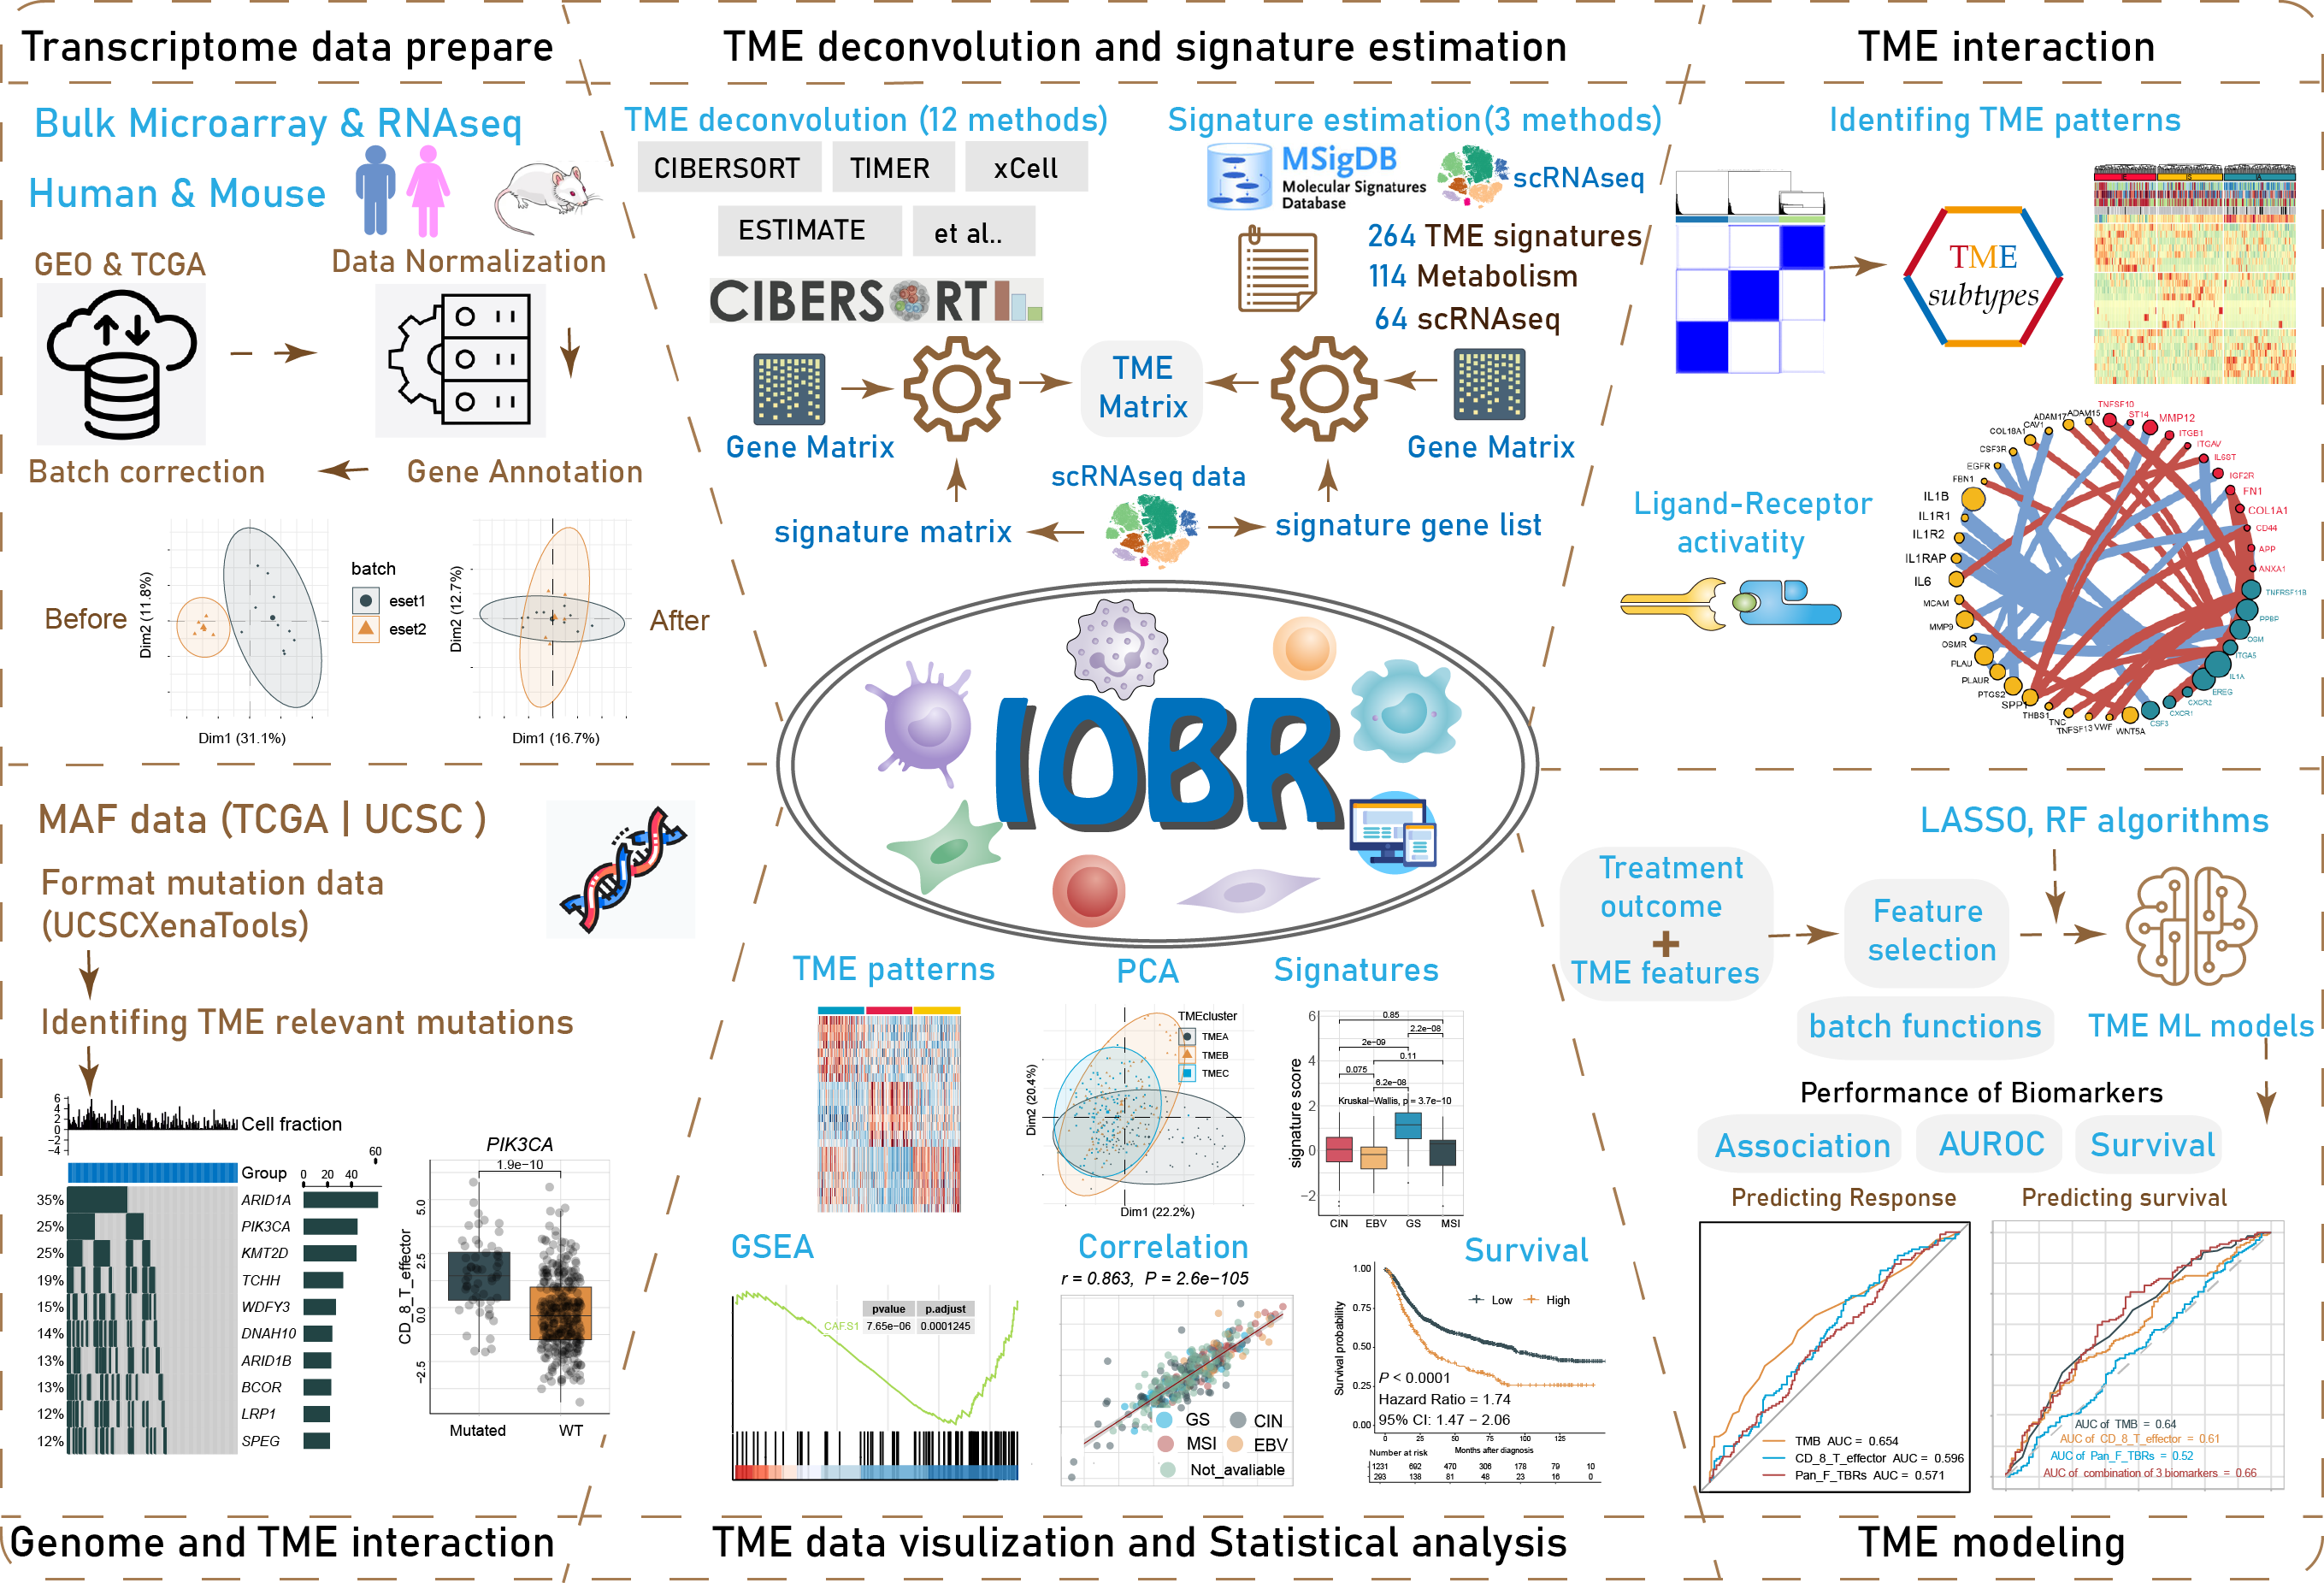
\includegraphics[width=0.95\linewidth]{./fig/IOBR-Workflow} 

}

\caption{The workflow of IOBR}\label{fig:unnamed-chunk-1}
\end{figure}

\hypertarget{introduction-1}{%
\section{Introduction}\label{introduction-1}}

IOBR is the acronym for \href{https://github.com/IOBR/IOBR}{Immuno-Oncology Biological Research}.
Recent advances in next-generation sequencing have triggered the rapid accumulation of publicly available multi-omics data. The application of integrated omics to explore robust signatures for clinical translation is increasingly highlighted in immuno-oncology, but poses computational and biological challenges. This vignette aims to demonstrate how to use the package named IOBR to perform multi-omics immuno-oncology biological research to decipher tumour microenvironment and signatures for clinical translation.

This R package integrates 8 published methods for decoding the tumour microenvironment (TME) context: \texttt{CIBERSORT}, \texttt{TIMER}, \texttt{xCell}, \texttt{MCPcounter}, \texttt{ESITMATE}, \texttt{EPIC}, \texttt{IPS}, \texttt{quanTIseq}. In addition, 264 published signature gene sets have been collected by IOBR covering tumour microenvironment, tumour metabolism, m6A, exosomes, microsatellite instability and tertiary lymphoid structure. The \texttt{signature\_collection\_citation} function is run to obtain the source papers, and the \texttt{signature\_collection} function returns the detailed signature genes of all given signatures. IOBR then uses three computational methods to calculate the signature score, including \texttt{PCA}, \texttt{z-score} and \texttt{ssGSEA}. Note that IOBR collected and used several approaches for variable transition, visualisation, batch survival analysis, feature selection and statistical analysis. Batch analysis and visualisation of results are supported. The details of how IOBR works are described below.

\hypertarget{license}{%
\section{License}\label{license}}

\textbf{IOBR} was released under the GPL v3.0 license. See \href{https://github.com/IOBR/IOBR/blob/master/LICENSE}{LICENSE} for details. The code contained in this book is simultaneously available under the \href{https://www.gnu.org/licenses/why-not-lgpl.html}{GPL license}; this means that you are free to use it in your packages, as long as you cite the source. The online version of this book is licensed under the \href{https://creativecommons.org/licenses/by-nc-sa/4.0/}{Creative Commons Attribution-NonCommercial-ShareAlike 4.0 International License.}

\hypertarget{previous-publication}{%
\section{Previous publication}\label{previous-publication}}

Zeng D, Ye Z, Shen R, Yu G, Wu J, Xiong Y,\ldots, Liao W (2021) \textbf{IOBR}: Multi-Omics Immuno-Oncology Biological Research to Decode Tumor Microenvironment and Signatures. \emph{Frontiers in Immunology}. 12:687975. \href{https://www.frontiersin.org/articles/10.3389/fimmu.2021.687975/full}{doi: 10.3389/fimmu.2021.687975}

Zeng D, Fang Y, \ldots, Liao W (2023) \textbf{IOBR2}: Multidimensional Decoding of Tumor Microenvironment for Immuno-Oncology Research. \emph{bioRxiv}.

\hypertarget{major-updates}{%
\section{Major Updates}\label{major-updates}}

\begin{figure}

{\centering 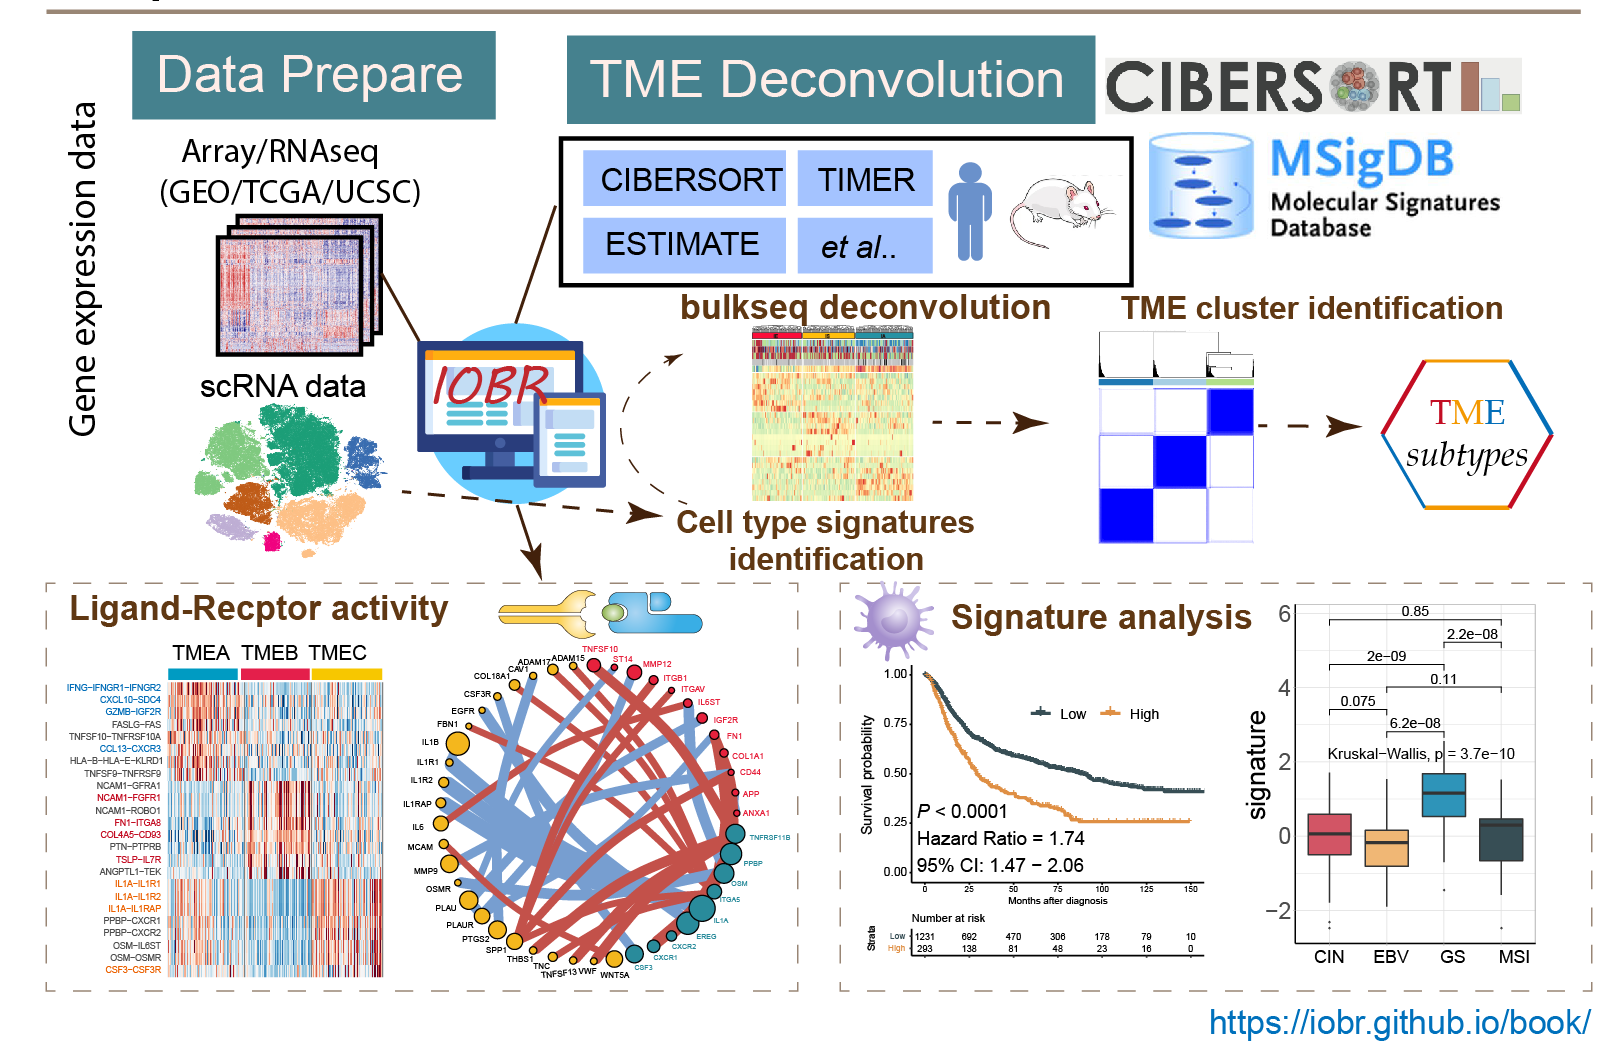
\includegraphics[width=0.95\linewidth]{./fig/IOBR-Workflow2} 

}

\caption{The workflow of IOBR}\label{fig:unnamed-chunk-2}
\end{figure}

\hypertarget{reporting-bugs}{%
\section{Reporting bugs}\label{reporting-bugs}}

Please report bugs to the \href{https://github.com/IOBR/IOBR/issues}{Github issues page}

E-mail any questions to Dr.~Fang \href{mailto:fyr_nate@163.com}{\nolinkurl{fyr\_nate@163.com}} or Dr.~Zeng \href{mailto:interlaken@smu.edu.cn}{\nolinkurl{interlaken@smu.edu.cn}}

\hypertarget{how-to-install-iobr}{%
\chapter{\texorpdfstring{\textbf{How to install IOBR}}{How to install IOBR}}\label{how-to-install-iobr}}

\hypertarget{install-dependency-packages}{%
\section{Install Dependency Packages}\label{install-dependency-packages}}

It is essential that you have R 3.6.3 or above already installed on your computer or server. IOBR is a pipeline that utilizes many other R packages that are currently available from CRAN, Bioconductor and GitHub.

\begin{Shaded}
\begin{Highlighting}[]
\ControlFlowTok{if}\NormalTok{ (}\SpecialCharTok{!}\FunctionTok{requireNamespace}\NormalTok{(}\StringTok{"BiocManager"}\NormalTok{, }\AttributeTok{quietly =} \ConstantTok{TRUE}\NormalTok{)) }\FunctionTok{install.packages}\NormalTok{(}\StringTok{"BiocManager"}\NormalTok{)}
\NormalTok{depens}\OtherTok{\textless{}{-}}\FunctionTok{c}\NormalTok{(}\StringTok{\textquotesingle{}tibble\textquotesingle{}}\NormalTok{, }\StringTok{\textquotesingle{}survival\textquotesingle{}}\NormalTok{, }\StringTok{\textquotesingle{}survminer\textquotesingle{}}\NormalTok{, }\StringTok{\textquotesingle{}limma\textquotesingle{}}\NormalTok{, }\StringTok{"DESeq2"}\NormalTok{,}\StringTok{"devtools"}\NormalTok{, }\StringTok{\textquotesingle{}limSolve\textquotesingle{}}\NormalTok{, }\StringTok{\textquotesingle{}GSVA\textquotesingle{}}\NormalTok{, }\StringTok{\textquotesingle{}e1071\textquotesingle{}}\NormalTok{, }\StringTok{\textquotesingle{}preprocessCore\textquotesingle{}}\NormalTok{, }
          \StringTok{"devtools"}\NormalTok{, }\StringTok{"tidyHeatmap"}\NormalTok{, }\StringTok{"caret"}\NormalTok{, }\StringTok{"glmnet"}\NormalTok{, }\StringTok{"ppcor"}\NormalTok{,  }\StringTok{"timeROC"}\NormalTok{, }\StringTok{"pracma"}\NormalTok{, }\StringTok{"factoextra"}\NormalTok{, }
          \StringTok{"FactoMineR"}\NormalTok{, }\StringTok{"WGCNA"}\NormalTok{, }\StringTok{"patchwork"}\NormalTok{, }\StringTok{\textquotesingle{}ggplot2\textquotesingle{}}\NormalTok{, }\StringTok{"biomaRt"}\NormalTok{, }\StringTok{\textquotesingle{}ggpubr\textquotesingle{}}\NormalTok{, }\StringTok{"PMCMRplus"}\NormalTok{)}
\ControlFlowTok{for}\NormalTok{(i }\ControlFlowTok{in} \DecValTok{1}\SpecialCharTok{:}\FunctionTok{length}\NormalTok{(depens))\{}
\NormalTok{  depen}\OtherTok{\textless{}{-}}\NormalTok{depens[i]}
  \ControlFlowTok{if}\NormalTok{ (}\SpecialCharTok{!}\FunctionTok{requireNamespace}\NormalTok{(depen, }\AttributeTok{quietly =} \ConstantTok{TRUE}\NormalTok{))  BiocManager}\SpecialCharTok{::}\FunctionTok{install}\NormalTok{(depen,}\AttributeTok{update =} \ConstantTok{FALSE}\NormalTok{)}
\NormalTok{\}}
\end{Highlighting}
\end{Shaded}

\hypertarget{install-iobr-package}{%
\section{Install IOBR package}\label{install-iobr-package}}

When the dependent environments are built, users are able to install IOBR from github by typing the following code into your R session:

\begin{Shaded}
\begin{Highlighting}[]
\ControlFlowTok{if}\NormalTok{ (}\SpecialCharTok{!}\FunctionTok{requireNamespace}\NormalTok{(}\StringTok{"IOBR"}\NormalTok{, }\AttributeTok{quietly =} \ConstantTok{TRUE}\NormalTok{))  devtools}\SpecialCharTok{::}\FunctionTok{install\_github}\NormalTok{(}\StringTok{"IOBR/IOBR"}\NormalTok{)}

\FunctionTok{library}\NormalTok{(IOBR)}
\end{Highlighting}
\end{Shaded}

\hypertarget{how-to-update-iobr}{%
\section{How to update IOBR}\label{how-to-update-iobr}}

\begin{Shaded}
\begin{Highlighting}[]
\FunctionTok{detach}\NormalTok{(}\StringTok{"package:IOBR"}\NormalTok{)}
\NormalTok{path}\OtherTok{\textless{}{-}}\FunctionTok{.libPaths}\NormalTok{()}
\FunctionTok{remove.packages}\NormalTok{(}\FunctionTok{c}\NormalTok{(}\StringTok{\textquotesingle{}IOBR\textquotesingle{}}\NormalTok{), }\AttributeTok{lib=}\FunctionTok{file.path}\NormalTok{(path))}
\NormalTok{devtools}\SpecialCharTok{::}\FunctionTok{install\_github}\NormalTok{(}\StringTok{"IOBR/IOBR"}\NormalTok{)}
\end{Highlighting}
\end{Shaded}

\hypertarget{how-to-use-iobr}{%
\chapter{\texorpdfstring{\textbf{How to use IOBR}}{How to use IOBR}}\label{how-to-use-iobr}}

\hypertarget{the-main-pipeline-of-iobr}{%
\section{The main pipeline of IOBR}\label{the-main-pipeline-of-iobr}}

\begin{figure}

{\centering 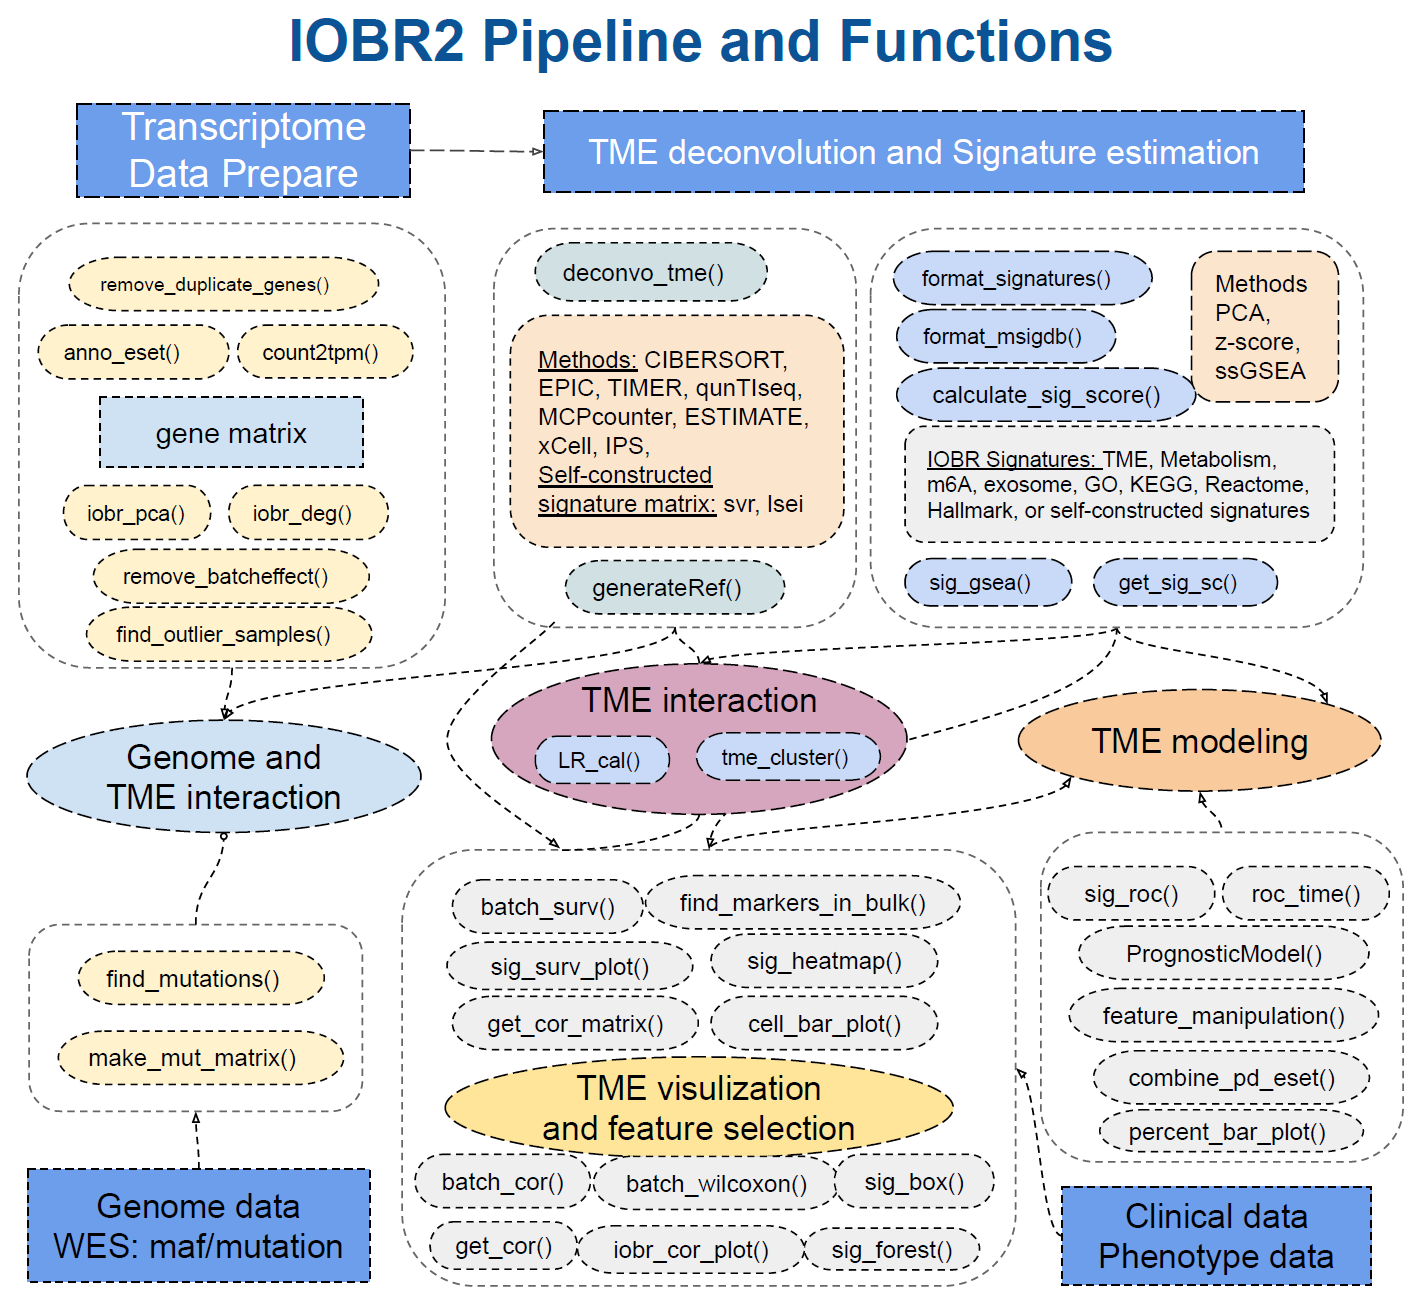
\includegraphics[width=0.95\linewidth]{./fig/IOBR-Package} 

}

\caption{The main pipeline of IOBR}\label{fig:flowchart}
\end{figure}

\hypertarget{main-functions-of-iobr}{%
\section{Main Functions of IOBR}\label{main-functions-of-iobr}}

\begin{itemize}
\item
  \textbf{Data Preparation: data annotation and transformation}

  \begin{itemize}
  \tightlist
  \item
    \texttt{count2tpm()}: transform gene expression count data into Transcripts Per Million (TPM) values. This function supports gene IDs of type ``Ensembl'', ``Entrez'', or ``Symbol'', and retrieves gene length information using either an online connection to the bioMart database or a local dataset (specified by the source parameter).
  \item
    \texttt{anno\_eset()}: annotate an ExpressionSet object (eset) with gene symbols using the provided annotation data. It retains only the rows with probes that have matching identifiers in the annotation data. The function handles duplicates according to the specified method. The output is an annotated and cleaned expression set.
  \item
    \texttt{remove\_duplicate\_genes()}: remove duplicate gene symbols from gene expression data. The retention of gene symbols is based either on their mean values (if method is set as ``mean'') or standard deviation values (if method is set as ``sd'').
  \item
    \texttt{mouse2human\_eset()}: convert mouse gene symbols to human gene symbols of expression set.
  \item
    \texttt{find\_outlier\_samples()}: analyze gene expression data and identify potential outlier samples based on connectivity analysis. By utilizing the ``WGCNA'' package, this function calculates the normalized adjacency and connectivity z-scores for each sample. It also offers multiple parameters to customize analysis and visualization.
  \item
    \texttt{remove\_batcheffect()}: remove batch effects from given expression datasets and visualize the corrected data using principal component analysis (PCA). It takes three expression datasets as input and performs batch effect correction using the ``sva::ComBat'' or ``sva::ComBat\_seq'' methods. The function then generates PCA plots to compare the data before and after correction.
  \end{itemize}
\item
  \textbf{TME Deconvolution Module: integrate multiple algorithms to decode immune contexture}

  \begin{itemize}
  \tightlist
  \item
    \texttt{deconvo\_tme()}: decode the TME infiltration using various deconvolution methodologies, based on bulk RNAseq, microarray or single cell RNAseq data. It currently supports methods include ``CIBERSORT'', ``MCPcounter'', ``EPIC'', ``xCell'', ``IPS'', ``estimate'', ``quanTIseq'', ``TIMER'', ``SVR'' and ``lsei''.
  \item
    \texttt{generateRef()}: generate a novel gene reference data for specific feature deconvolution, such as infiltrating cell, utilizing different methods to identify differentially expressed genes (DEGs) . The function supports both ``limma'' and ``DESeq2'' methods.The resulting gene reference data can be used for \texttt{deconvo\_tme()} with the ``SVR'' and ``lsei'' algorithms.
  \item
    \texttt{generateRef\_seurat()}: take a Seurat object ``sce'' and additional parameters to perform various operations for generating reference gene expression data. It allows for specifying cell types, proportions, assays, preprocessing options, and statistical testing parameters.The resulting gene reference data can be used for \texttt{deconvo\_tme()} with the ``svr'' and ``lsei'' algorithms.
  \end{itemize}
\item
  \textbf{Signature Module: calculatint signature scores, estimate phenotype related signatures and corresponding genes, and evaluate signatures generated from single-cell RNA sequencing data }

  \begin{itemize}
  \tightlist
  \item
    \texttt{calculate\_sig\_score()}: estimate the interested signatures enrolled in IOBR R package, which involves TME-associated, tumor-metabolism, and tumor-intrinsic signatures.The supported methods for signature score calculation include ``PCA'', ``ssGSEA'', ``z-score'', and Integration.
  \item
    \texttt{feature\_manipulation()}: manipulate features including the cell fraction and signatures generated from multi-omics data for latter analysis and model construction. Remove missing values, outliers and variables without significant variance.
  \item
    \texttt{format\_signatures()}: generate the object for \texttt{calculate\_sig\_score()} function, by inputting a data frame with signatures as column names of corresponding gene sets, and return a list contain the signature information for calculating multiple signature scores.
  \item
    \texttt{format\_msigdb()}: transform the signature gene sets data with gmt format, which is not included in the signature collection and might be downloaded in the MSgiDB website, into the object of \texttt{calculate\_sig\_score()}function.
  \item
    \texttt{sig\_gsea()}: conduct Gene Set Enrichment Analysis (GSEA) to identify significant gene sets based on differential gene expression data. This function performs GSEA using the fgsea package and provides visualizations and results in the form of tables and plots. It supports the utilization of user-defined gene sets or the use of predefined gene sets from MSigDB.
  \item
    \texttt{get\_sig\_sc()}: get top gene signatures from single-cell differential analysis for \texttt{calculate\_sig\_score()} function. The input is a matrix containing a ranked list of putative markers, and associated statistics (p-values, ROC score, etc.)
  \end{itemize}
\item
  \textbf{Batch Analysis and Visualization: batch survival analysis and batch correlation analysis and other batch statistical analyses }

  \begin{itemize}
  \tightlist
  \item
    \texttt{batch\_surv()}: perform batch survival analysis. It calculates hazard ratios and confidence intervals for the specified variables based on the given data containing time-related information.
  \item
    \texttt{subgroup\_survival()}: extract hazard ratio and confidence intervals from a coxph object of subgroup analysis.
  \item
    \texttt{batch\_cor()}: batch analysis of correlation between two continuous variables using Pearson correlation coefficient or Spearman's rank correlation coefficient.
  \item
    \texttt{batch\_wilcoxon()}: perform Wilcoxon rank-sum tests on a given data set to compare the distribution of a specified feature between two groups. It computes the p-values and ranks the significant features based on the p-values. It returns a data frame with the feature names, p-values, adjusted p-values, logarithm of p-values, and a star rating based on the p-value ranges.
  \item
    \texttt{batch\_pcc()}: provide a batch way to calculate the partial correlation coefficient between feature and others when controlling a third variable.
  \item
    \texttt{iobr\_cor\_plot()}: visualization of batch correlation analysis of signatures from ``sig\_group''. Visualize the correlation between signature or phenotype with expression of gene sets in target signature is also supported.
  \item
    \texttt{cell\_bar\_plot()}: batch visualization of TME cell fraction, supporting input of deconvolution results from ``CIBERSORT'', ``EPIC'' and ``quanTIseq'' methodologies to further compare the TME cell distributions within one sample or among different samples.
  \item
    \texttt{iobr\_pca()}: perform Principal Component Analysis (PCA), which reduces the dimensionality of data while maintaining most of the original variance, and visualizes the PCA results on a scatter plot.
  \item
    \texttt{iobr\_deg()}: perform differential expression analysis on gene expression data using the DESeq2 or limma method. It filters low count data, calculates fold changes and adjusted p-values, and identifies DEGs based on specified cutoffs. It also provides optional visualization tools such as volcano plots and heatmaps.
  \item
    \texttt{get\_cor()}: calculate and visualize the correlation between two variables in a dataset. It provides options to scale the data, handle missing values, and incorporate additional data. The function supports various correlation methods. It generates a correlation plot with optional subtypes or categories, including a regression line.
  \item
    \texttt{get\_cor\_matrix()}: calculate and visualize the correlation matrix between two sets of variables in a dataset. It provides flexibility in defining correlation methods, handling missing values, and incorporating additional data. The function supports various correlation methods, such as Pearson correlation, and displays the correlation result in a customizable plot.
  \item
    \texttt{roc\_time()}: generate a Receiver Operating Characteristic (ROC) plot over time to assess the predictive performance of one or more variables in survival analysis. It calculates the Area Under the Curve (AUC) for each specified time point and variable combination, and creates a multi-line ROC plot with corresponding AUC values annotated.
  \item
    \texttt{sig\_box()}: generate a boxplot with optional statistical comparisons. It takes in various parameters such as data, signature, variable, and more to customize the plot. It can be used to visualize and analyze data in a Seurat object or any other data frame.
  \item
    \texttt{sig\_heatmap()}: generate a heatmap plot based on input data, grouping variables, and optional conditions. The function allows customization of various parameters such as palette selection, scaling, color boxes, plot dimensions, and more. It provides flexibility in visualizing relationships between variables and groups in a concise and informative manner.
  \item
    \texttt{sig\_forest()}: create a forest plot for visualizing survival analysis results generated by ``batch\_surv''.
  \item
    \texttt{sig\_roc()}: plot multiple ROC curves in a single graph, facilitating the comparison of different variables in terms of their ability to predict a binary response.
  \item
    \texttt{sig\_surv\_plot()}: generat multiple Kaplan-Meier (KM) survival plots for a given signature or gene. It allows for detailed customization and is structured to handle various aspects of survival analysis.
  \item
    \texttt{find\_markers\_in\_bulk()}: find relevant results from the given gene expression data and meta information. It leverages the ``Seurat'' package to identify significant markers across multiple groups within the given data. The supported methods for comparison include ``bootstrap'', ``delong'' and ``venkatraman''.
  \end{itemize}
\item
  \textbf{Signature Associated Mutation Module: identify and analyze mutations relevant to targeted signatures}

  \begin{itemize}
  \tightlist
  \item
    \texttt{make\_mut\_matrix()}: transform the mutation data with MAF format(contain the columns of gene ID and the corresponding gene alterations which including SNP, indel and frameshift) into a mutation matrix in a suitable manner for further investigating signature relevant mutations.
  \item
    \texttt{find\_mutations()}: identify mutations associated with a distinct phenotype or signature. The function conducts the Cuzick test, Wilcoxon test, or both (when the method is set to ``multi''). It generates box plots for the top genes identified through these statistical tests and creates oncoprints to graphically represent the mutation landscape across samples.
  \end{itemize}
\item
  \textbf{Model Construction Module: feature selection and fast model construct to predict clinical phenotype}

  \begin{itemize}
  \tightlist
  \item
    \texttt{BinomialModel()}: select features and construct a model to predict a binary phenotype. It accepts a dataset (x and y) as input and performs data processing, splitting into training and testing sets, and model fitting using both Lasso and Ridge regression techniques.
  \item
    \texttt{PrognosticMode()}: select features and construct a model to predict clinical survival outcome. It primarily focuses on developing Lasso and Ridge regression models within the Cox proportional hazards framework.
  \item
    \texttt{combine\_pd\_eset()}: combine the expression set (eset) with phenotype data (pdata).
  \item
    \texttt{percent\_bar\_plot()}: create a percent bar plot based on the given data. The input is a data frame, with x and y-axis variables specified.
  \end{itemize}
\end{itemize}

\hypertarget{current-working-environment}{%
\section{Current working environment}\label{current-working-environment}}

\begin{Shaded}
\begin{Highlighting}[]
\FunctionTok{sessionInfo}\NormalTok{()}
\end{Highlighting}
\end{Shaded}

\begin{verbatim}
## R version 4.2.0 (2022-04-22 ucrt)
## Platform: x86_64-w64-mingw32/x64 (64-bit)
## Running under: Windows 10 x64 (build 19045)
## 
## Matrix products: default
## 
## locale:
## [1] LC_COLLATE=Chinese (Simplified)_China.utf8 
## [2] LC_CTYPE=Chinese (Simplified)_China.utf8   
## [3] LC_MONETARY=Chinese (Simplified)_China.utf8
## [4] LC_NUMERIC=C                               
## [5] LC_TIME=Chinese (Simplified)_China.utf8    
## 
## attached base packages:
## [1] stats     graphics  grDevices utils     datasets  methods   base     
## 
## loaded via a namespace (and not attached):
##  [1] compiler_4.2.0    fastmap_1.1.1     bookdown_0.36     cli_3.6.1        
##  [5] htmltools_0.5.6.1 tools_4.2.0       rstudioapi_0.15.0 yaml_2.3.7       
##  [9] rmarkdown_2.25    knitr_1.45        digest_0.6.29     xfun_0.40        
## [13] rlang_1.1.1       evaluate_0.22
\end{verbatim}

\hypertarget{rna-data-preprocessing}{%
\chapter{\texorpdfstring{\textbf{RNA Data preprocessing}}{RNA Data preprocessing}}\label{rna-data-preprocessing}}

\hypertarget{loading-packages}{%
\section{Loading packages}\label{loading-packages}}

Load the IOBR package in your R session after the installation is complete:

\begin{Shaded}
\begin{Highlighting}[]
\FunctionTok{library}\NormalTok{(IOBR)}
\FunctionTok{library}\NormalTok{(tidyverse)}
\FunctionTok{library}\NormalTok{(clusterProfiler)}
\end{Highlighting}
\end{Shaded}

\hypertarget{download-array-data-using-geoquery}{%
\section{\texorpdfstring{Download array data using \texttt{GEOquery}}{Download array data using GEOquery}}\label{download-array-data-using-geoquery}}

Obtaining data set from GEO \href{https://pubmed.ncbi.nlm.nih.gov/25894828/}{Gastric cancer: GSE62254} using \texttt{GEOquery} R package.

\begin{Shaded}
\begin{Highlighting}[]
\ControlFlowTok{if}\NormalTok{ (}\SpecialCharTok{!}\FunctionTok{requireNamespace}\NormalTok{(}\StringTok{"GEOquery"}\NormalTok{, }\AttributeTok{quietly =} \ConstantTok{TRUE}\NormalTok{))  BiocManager}\SpecialCharTok{::}\FunctionTok{install}\NormalTok{(}\StringTok{"GEOquery"}\NormalTok{)}
\FunctionTok{library}\NormalTok{(}\StringTok{"GEOquery"}\NormalTok{)}
\CommentTok{\# }\AlertTok{NOTE}\CommentTok{: This process may take a few minutes which depends on the internet connection speed. Please wait for its completion.}
\NormalTok{eset\_geo}\OtherTok{\textless{}{-}}\FunctionTok{getGEO}\NormalTok{(}\AttributeTok{GEO     =} \StringTok{"GSE62254"}\NormalTok{, }\AttributeTok{getGPL  =}\NormalTok{ F, }\AttributeTok{destdir =} \StringTok{"./"}\NormalTok{)}
\NormalTok{eset    }\OtherTok{\textless{}{-}}\NormalTok{eset\_geo[[}\DecValTok{1}\NormalTok{]]}
\NormalTok{eset    }\OtherTok{\textless{}{-}}\FunctionTok{exprs}\NormalTok{(eset)}
\NormalTok{eset[}\DecValTok{1}\SpecialCharTok{:}\DecValTok{5}\NormalTok{,}\DecValTok{1}\SpecialCharTok{:}\DecValTok{5}\NormalTok{]}
\end{Highlighting}
\end{Shaded}

\begin{verbatim}
##           GSM1523727 GSM1523728 GSM1523729 GSM1523744 GSM1523745
## 1007_s_at  3.2176645  3.0624323  3.0279131   2.921683  2.8456013
## 1053_at    2.4050109  2.4394879  2.2442708   2.345916  2.4328582
## 117_at     1.4933412  1.8067380  1.5959665   1.839822  1.8326058
## 121_at     2.1965561  2.2812181  2.1865556   2.258599  2.1874363
## 1255_g_at  0.8698382  0.9502466  0.8125414   1.012860  0.9441993
\end{verbatim}

\hypertarget{gene-annotation}{%
\section{Gene Annotation}\label{gene-annotation}}

Annotation of genes in the expression matrix and removal of duplicate genes.

\begin{Shaded}
\begin{Highlighting}[]
\CommentTok{\# Load the annotation file \textasciigrave{}anno\_hug133plus2\textasciigrave{} in IOBR.}
\FunctionTok{head}\NormalTok{(anno\_hug133plus2)}
\end{Highlighting}
\end{Shaded}

\begin{verbatim}
## # A tibble: 6 x 2
##   probe_id  symbol 
##   <fct>     <fct>  
## 1 1007_s_at MIR4640
## 2 1053_at   RFC2   
## 3 117_at    HSPA6  
## 4 121_at    PAX8   
## 5 1255_g_at GUCA1A 
## 6 1294_at   MIR5193
\end{verbatim}

\begin{Shaded}
\begin{Highlighting}[]
\CommentTok{\# Load the annotation file \textasciigrave{}anno\_grch38\textasciigrave{} in IOBR.}
\FunctionTok{head}\NormalTok{(anno\_grch38)}
\end{Highlighting}
\end{Shaded}

\begin{verbatim}
##                id eff_length        gc entrez   symbol chr     start       end
## 1 ENSG00000000003       4536 0.3992504   7105   TSPAN6   X 100627109 100639991
## 2 ENSG00000000005       1476 0.4241192  64102     TNMD   X 100584802 100599885
## 3 ENSG00000000419       9276 0.4252911   8813     DPM1  20  50934867  50958555
## 4 ENSG00000000457       6883 0.4117391  57147    SCYL3   1 169849631 169894267
## 5 ENSG00000000460       5970 0.4298157  55732 C1orf112   1 169662007 169854080
## 6 ENSG00000000938       3382 0.5644589   2268      FGR   1  27612064  27635277
##   strand        biotype
## 1     -1 protein_coding
## 2      1 protein_coding
## 3     -1 protein_coding
## 4     -1 protein_coding
## 5      1 protein_coding
## 6     -1 protein_coding
##                                                                                                  description
## 1                                                          tetraspanin 6 [Source:HGNC Symbol;Acc:HGNC:11858]
## 2                                                            tenomodulin [Source:HGNC Symbol;Acc:HGNC:17757]
## 3 dolichyl-phosphate mannosyltransferase polypeptide 1, catalytic subunit [Source:HGNC Symbol;Acc:HGNC:3005]
## 4                                               SCY1-like, kinase-like 3 [Source:HGNC Symbol;Acc:HGNC:19285]
## 5                                    chromosome 1 open reading frame 112 [Source:HGNC Symbol;Acc:HGNC:25565]
## 6                          FGR proto-oncogene, Src family tyrosine kinase [Source:HGNC Symbol;Acc:HGNC:3697]
\end{verbatim}

\begin{Shaded}
\begin{Highlighting}[]
\CommentTok{\# Load the annotation file \textasciigrave{}anno\_gc\_vm32\textasciigrave{} in IOBR for mouse RNAseq data}
\FunctionTok{head}\NormalTok{(anno\_gc\_vm32)}
\end{Highlighting}
\end{Shaded}

\begin{verbatim}
##                   id eff_length        gc symbol      mgi_id      gene_type
## 1 ENSMUSG00000000001       3262 0.4350092  Gnai3   MGI:95773 protein_coding
## 2 ENSMUSG00000000003        902 0.3481153   Pbsn MGI:1860484 protein_coding
## 3 ENSMUSG00000000028       3506 0.4962921  Cdc45 MGI:1338073 protein_coding
## 4 ENSMUSG00000000031       2625 0.5588571    H19   MGI:95891         lncRNA
## 5 ENSMUSG00000000037       6397 0.4377052  Scml2 MGI:1340042 protein_coding
## 6 ENSMUSG00000000049       1594 0.5050188   Apoh   MGI:88058 protein_coding
##       start       end transcript_id  ont
## 1 108014596 108053462          <NA> <NA>
## 2  76881507  76897229          <NA> <NA>
## 3  18599197  18630737          <NA> <NA>
## 4 142129262 142131886          <NA> <NA>
## 5 159865521 160041209          <NA> <NA>
## 6 108234180 108305222          <NA> <NA>
\end{verbatim}

\hypertarget{for-array-data-hgu133plus-2-affaymetrix}{%
\subsection{For Array data: HGU133PLUS-2 (Affaymetrix)}\label{for-array-data-hgu133plus-2-affaymetrix}}

\begin{Shaded}
\begin{Highlighting}[]
\CommentTok{\# Conduct gene annotation using \textasciigrave{}anno\_hug133plus2\textasciigrave{} file; If identical gene symbols exists, these genes would be ordered by the mean expression levels. The gene symbol with highest mean expression level is selected and remove others. }

\NormalTok{eset}\OtherTok{\textless{}{-}}\FunctionTok{anno\_eset}\NormalTok{(}\AttributeTok{eset       =}\NormalTok{ eset,}
                \AttributeTok{annotation =}\NormalTok{ anno\_hug133plus2,}
                \AttributeTok{symbol     =} \StringTok{"symbol"}\NormalTok{,}
                \AttributeTok{probe      =} \StringTok{"probe\_id"}\NormalTok{,}
                \AttributeTok{method     =} \StringTok{"mean"}\NormalTok{)}
\NormalTok{eset[}\DecValTok{1}\SpecialCharTok{:}\DecValTok{5}\NormalTok{, }\DecValTok{1}\SpecialCharTok{:}\DecValTok{3}\NormalTok{]}
\end{Highlighting}
\end{Shaded}

\begin{verbatim}
##              GSM1523727 GSM1523728 GSM1523729
## SH3KBP1        4.327974   4.316195   4.351425
## RPL41          4.246149   4.246808   4.257940
## EEF1A1         4.293762   4.291038   4.262199
## COX2           4.250288   4.283714   4.270508
## LOC101928826   4.219303   4.219670   4.213252
\end{verbatim}

\hypertarget{download-rnaseq-data-using-ucscxenatools}{%
\section{\texorpdfstring{Download RNAseq data using \texttt{UCSCXenaTools}}{Download RNAseq data using UCSCXenaTools}}\label{download-rnaseq-data-using-ucscxenatools}}

\begin{Shaded}
\begin{Highlighting}[]
\ControlFlowTok{if}\NormalTok{ (}\SpecialCharTok{!}\FunctionTok{requireNamespace}\NormalTok{(}\StringTok{"UCSCXenaTools"}\NormalTok{, }\AttributeTok{quietly =} \ConstantTok{TRUE}\NormalTok{))   BiocManager}\SpecialCharTok{::}\FunctionTok{install}\NormalTok{(}\StringTok{"UCSCXenaTools"}\NormalTok{)}
\FunctionTok{library}\NormalTok{(UCSCXenaTools)}
\CommentTok{\# }\AlertTok{NOTE}\CommentTok{: This process may take a few minutes which depends on the internet connection speed. Please wait for its completion.}
\NormalTok{eset\_stad}\OtherTok{\textless{}{-}}\FunctionTok{XenaGenerate}\NormalTok{(}\AttributeTok{subset =}\NormalTok{ XenaCohorts }\SpecialCharTok{==}\StringTok{"GDC TCGA Stomach Cancer (STAD)"}\NormalTok{) }\SpecialCharTok{\%\textgreater{}\%} 
  \FunctionTok{XenaFilter}\NormalTok{(}\AttributeTok{filterDatasets    =} \StringTok{"TCGA{-}STAD.htseq\_counts.tsv"}\NormalTok{) }\SpecialCharTok{\%\textgreater{}\%} 
  \FunctionTok{XenaQuery}\NormalTok{() }\SpecialCharTok{\%\textgreater{}\%}
  \FunctionTok{XenaDownload}\NormalTok{() }\SpecialCharTok{\%\textgreater{}\%} 
  \FunctionTok{XenaPrepare}\NormalTok{()}
\NormalTok{eset\_stad[}\DecValTok{1}\SpecialCharTok{:}\DecValTok{5}\NormalTok{, }\DecValTok{1}\SpecialCharTok{:}\DecValTok{3}\NormalTok{]}
\end{Highlighting}
\end{Shaded}

\hypertarget{normalization-and-gene-annotation}{%
\section{Normalization and Gene annotation}\label{normalization-and-gene-annotation}}

Transform gene expression matrix into TPM format, and conduct subsequent annotation.

\begin{Shaded}
\begin{Highlighting}[]
\CommentTok{\# Remove the version numbers in Ensembl ID.}
\NormalTok{eset\_stad}\SpecialCharTok{$}\NormalTok{Ensembl\_ID}\OtherTok{\textless{}{-}}\FunctionTok{substring}\NormalTok{(eset\_stad}\SpecialCharTok{$}\NormalTok{Ensembl\_ID, }\DecValTok{1}\NormalTok{, }\DecValTok{15}\NormalTok{)}
\NormalTok{eset\_stad}\OtherTok{\textless{}{-}}\FunctionTok{column\_to\_rownames}\NormalTok{(eset\_stad, }\AttributeTok{var =} \StringTok{"Ensembl\_ID"}\NormalTok{)}

\CommentTok{\# Revert back to original format because the data from UCSC was log2(x+1)transformed.}
\NormalTok{eset\_stad}\OtherTok{\textless{}{-}}\NormalTok{(}\DecValTok{2}\SpecialCharTok{\^{}}\NormalTok{eset\_stad)}\SpecialCharTok{+}\DecValTok{1}

\NormalTok{eset\_stad}\OtherTok{\textless{}{-}}\FunctionTok{count2tpm}\NormalTok{(}\AttributeTok{countMat =}\NormalTok{ eset\_stad, }\AttributeTok{idType =} \StringTok{"Ensembl"}\NormalTok{, }\AttributeTok{org=}\StringTok{"hsa"}\NormalTok{, }\AttributeTok{source =} \StringTok{"local"}\NormalTok{ )}

\NormalTok{eset\_stad[}\DecValTok{1}\SpecialCharTok{:}\DecValTok{5}\NormalTok{,}\DecValTok{1}\SpecialCharTok{:}\DecValTok{5}\NormalTok{]}
\end{Highlighting}
\end{Shaded}

\hypertarget{identifying-outlier-samples}{%
\section{Identifying outlier samples}\label{identifying-outlier-samples}}

Take ACRG microarray data for example

\begin{Shaded}
\begin{Highlighting}[]
\NormalTok{res }\OtherTok{\textless{}{-}} \FunctionTok{find\_outlier\_samples}\NormalTok{(}\AttributeTok{eset =}\NormalTok{ eset, }\AttributeTok{project =} \StringTok{"ACRG"}\NormalTok{, }\AttributeTok{show\_plot =} \ConstantTok{TRUE}\NormalTok{)}
\end{Highlighting}
\end{Shaded}

\begin{center}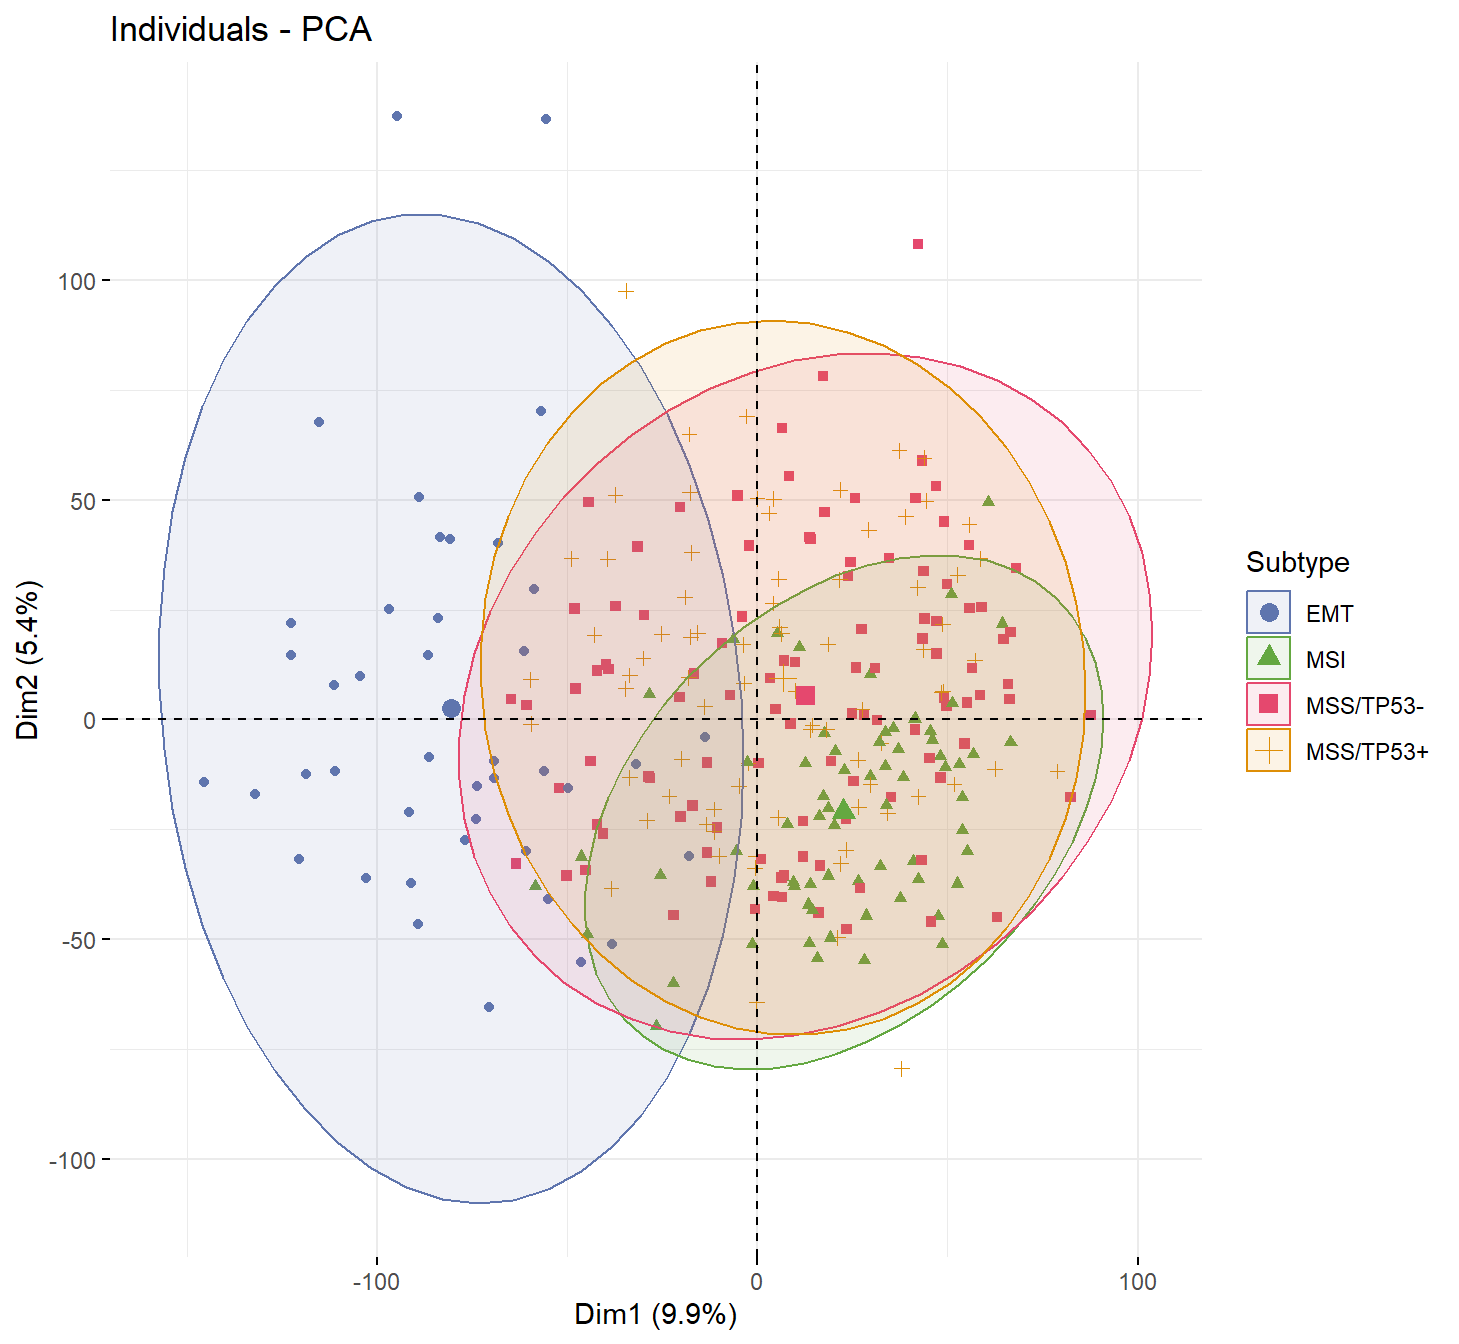
\includegraphics{data-preprocessing_files/figure-latex/unnamed-chunk-9-1} \end{center}

\begin{verbatim}
## [1] "GSM1523817" "GSM1523858" "GSM1523984" "GSM1523988" "GSM1524030"
\end{verbatim}

Removing potential outlier samples

\begin{Shaded}
\begin{Highlighting}[]
\NormalTok{eset1 }\OtherTok{\textless{}{-}}\NormalTok{ eset[, }\SpecialCharTok{!}\FunctionTok{colnames}\NormalTok{(eset)}\SpecialCharTok{\%in\%}\NormalTok{res]}
\end{Highlighting}
\end{Shaded}

\hypertarget{pca-analysis-of-molecular-subtypes}{%
\section{PCA analysis of molecular subtypes}\label{pca-analysis-of-molecular-subtypes}}

\begin{Shaded}
\begin{Highlighting}[]
\FunctionTok{data}\NormalTok{(}\StringTok{"pdata\_acrg"}\NormalTok{)}
\NormalTok{res}\OtherTok{\textless{}{-}} \FunctionTok{iobr\_pca}\NormalTok{(}\AttributeTok{data       =}\NormalTok{ eset1,}
              \AttributeTok{is.matrix   =} \ConstantTok{TRUE}\NormalTok{,}
              \AttributeTok{scale       =} \ConstantTok{TRUE}\NormalTok{,}
              \AttributeTok{is.log      =} \ConstantTok{FALSE}\NormalTok{,}
              \AttributeTok{pdata       =}\NormalTok{ pdata\_acrg, }
              \AttributeTok{id\_pdata    =} \StringTok{"ID"}\NormalTok{, }
              \AttributeTok{group       =} \StringTok{"Subtype"}\NormalTok{,}
              \AttributeTok{geom.ind    =} \StringTok{"point"}\NormalTok{, }
              \AttributeTok{cols        =} \StringTok{"normal"}\NormalTok{,}
              \AttributeTok{palette     =} \StringTok{"jama"}\NormalTok{, }
              \AttributeTok{repel       =} \ConstantTok{FALSE}\NormalTok{,}
              \AttributeTok{ncp         =} \DecValTok{5}\NormalTok{,}
              \AttributeTok{axes        =} \FunctionTok{c}\NormalTok{(}\DecValTok{1}\NormalTok{, }\DecValTok{2}\NormalTok{),}
              \AttributeTok{addEllipses =} \ConstantTok{TRUE}\NormalTok{)}
\end{Highlighting}
\end{Shaded}

\begin{verbatim}
## 
##       CIN       EBV       EMT        GS       MSI MSS/TP53- MSS/TP53+ 
##         0         0        42         0        68       106        79 
## [1] ">>-- colors for PCA: "
\end{verbatim}

\begin{Shaded}
\begin{Highlighting}[]
\NormalTok{res}
\end{Highlighting}
\end{Shaded}

\begin{center}\includegraphics{data-preprocessing_files/figure-latex/unnamed-chunk-11-1} \end{center}

\hypertarget{batch-effect-correction}{%
\section{Batch effect correction}\label{batch-effect-correction}}

\hypertarget{for-microarray-data}{%
\subsection{For microarray data}\label{for-microarray-data}}

Obtaining another data set from GEO \href{https://www.ncbi.nlm.nih.gov/pubmed/24935174/}{Gastric cancer: GSE57303} using \texttt{GEOquery} R package.

\begin{Shaded}
\begin{Highlighting}[]
\CommentTok{\# }\AlertTok{NOTE}\CommentTok{: This process may take a few minutes which depends on the internet connection speed. Please wait for its completion.}
\NormalTok{eset\_geo}\OtherTok{\textless{}{-}}\FunctionTok{getGEO}\NormalTok{(}\AttributeTok{GEO     =} \StringTok{"GSE57303"}\NormalTok{, }\AttributeTok{getGPL  =}\NormalTok{ F, }\AttributeTok{destdir =} \StringTok{"./"}\NormalTok{)}
\NormalTok{eset2    }\OtherTok{\textless{}{-}}\NormalTok{eset\_geo[[}\DecValTok{1}\NormalTok{]]}
\NormalTok{eset2    }\OtherTok{\textless{}{-}}\FunctionTok{exprs}\NormalTok{(eset2)}
\NormalTok{eset2[}\DecValTok{1}\SpecialCharTok{:}\DecValTok{5}\NormalTok{,}\DecValTok{1}\SpecialCharTok{:}\DecValTok{5}\NormalTok{]}
\end{Highlighting}
\end{Shaded}

\begin{verbatim}
##           GSM1379261 GSM1379262 GSM1379263 GSM1379264 GSM1379265
## 1007_s_at    8.34746    9.67994    8.62643    8.59301    8.63046
## 1053_at      5.07972    4.46377    5.29685    5.78983    4.33359
## 117_at       5.65558    4.48732    4.21615    5.47984    5.20816
## 121_at       5.95123    7.09056    6.19903    5.89872    5.91323
## 1255_g_at    1.66923    1.98758    1.73083    1.56687    1.63332
\end{verbatim}

Annotation of genes in the expression matrix and removal of duplicate genes.

\begin{Shaded}
\begin{Highlighting}[]
\NormalTok{eset2}\OtherTok{\textless{}{-}}\FunctionTok{anno\_eset}\NormalTok{(}\AttributeTok{eset       =}\NormalTok{ eset2,}
                 \AttributeTok{annotation =}\NormalTok{ anno\_hug133plus2,}
                 \AttributeTok{symbol     =} \StringTok{"symbol"}\NormalTok{,}
                 \AttributeTok{probe      =} \StringTok{"probe\_id"}\NormalTok{,}
                 \AttributeTok{method     =} \StringTok{"mean"}\NormalTok{)}
\NormalTok{eset2[}\DecValTok{1}\SpecialCharTok{:}\DecValTok{5}\NormalTok{, }\DecValTok{1}\SpecialCharTok{:}\DecValTok{5}\NormalTok{]}
\end{Highlighting}
\end{Shaded}

\begin{verbatim}
##         GSM1379261 GSM1379262 GSM1379263 GSM1379264 GSM1379265
## ND4        13.1695    13.1804    13.0600    12.4544    13.0457
## ATP6       13.1433    13.0814    13.0502    12.4831    13.1168
## SH3KBP1    12.9390    13.1620    12.9773    12.8745    13.1169
## COX2       13.0184    13.0489    12.8621    12.7489    12.9732
## RPL41      13.0201    12.6034    12.7929    13.0153    12.9404
\end{verbatim}

\begin{Shaded}
\begin{Highlighting}[]
\NormalTok{eset\_com }\OtherTok{\textless{}{-}} \FunctionTok{remove\_batcheffect}\NormalTok{( }\AttributeTok{eset1       =}\NormalTok{ eset1,  }
                                \AttributeTok{eset2       =}\NormalTok{ eset2,   }
                                \AttributeTok{eset3       =} \ConstantTok{NULL}\NormalTok{,}
                                \AttributeTok{id\_type     =} \StringTok{"symbol"}\NormalTok{,}
                                \AttributeTok{data\_type   =} \StringTok{"array"}\NormalTok{, }
                                \AttributeTok{cols        =} \StringTok{"normal"}\NormalTok{, }
                                \AttributeTok{palette     =} \StringTok{"jama"}\NormalTok{, }
                                \AttributeTok{log2        =} \ConstantTok{TRUE}\NormalTok{, }
                                \AttributeTok{check\_eset  =} \ConstantTok{TRUE}\NormalTok{,}
                                \AttributeTok{adjust\_eset =} \ConstantTok{TRUE}\NormalTok{,}
                                \AttributeTok{repel       =} \ConstantTok{FALSE}\NormalTok{,}
                                \AttributeTok{path        =} \StringTok{"result"}\NormalTok{)}
\end{Highlighting}
\end{Shaded}

\begin{verbatim}
## 
## eset1 eset2 
##   295    70 
## [1] ">>-- colors for PCA: "
## 
## eset1 eset2 
##   295    70 
## [1] ">>-- colors for PCA: "
\end{verbatim}

\begin{center}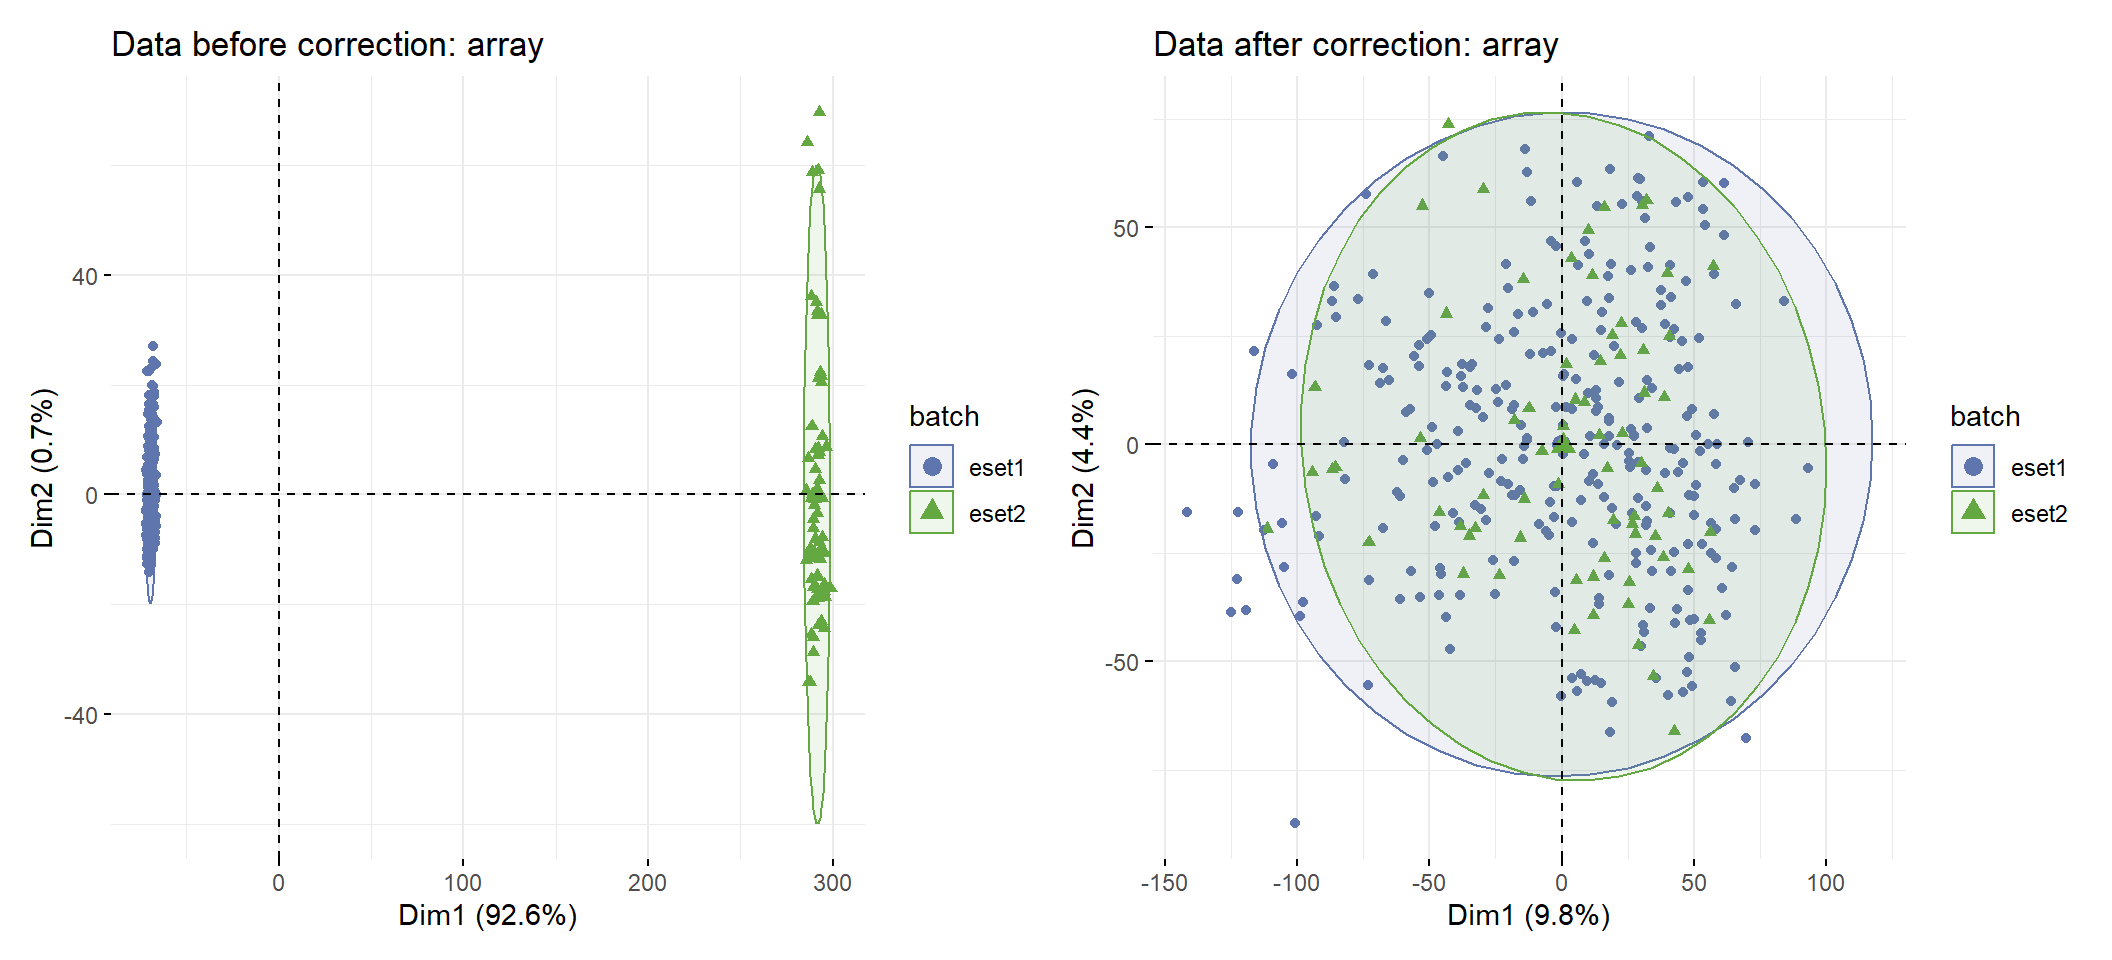
\includegraphics{data-preprocessing_files/figure-latex/unnamed-chunk-14-1} \end{center}

\begin{Shaded}
\begin{Highlighting}[]
\FunctionTok{dim}\NormalTok{(eset\_com)}
\end{Highlighting}
\end{Shaded}

\begin{verbatim}
## [1] 21752   365
\end{verbatim}

\hypertarget{for-rnaseq-count-data}{%
\subsection{For RNAseq count data}\label{for-rnaseq-count-data}}

\begin{Shaded}
\begin{Highlighting}[]
\FunctionTok{data}\NormalTok{(}\StringTok{"eset\_stad"}\NormalTok{, }\AttributeTok{package =} \StringTok{"IOBR"}\NormalTok{)}
\FunctionTok{head}\NormalTok{(eset\_stad)}
\end{Highlighting}
\end{Shaded}

\begin{verbatim}
##                 TCGA-BR-6455 TCGA-BR-7196 TCGA-BR-8371 TCGA-BR-8380
## ENSG00000000003         8006         2114          767         1556
## ENSG00000000005            1            0            5            5
## ENSG00000000419         3831         2600         1729         1760
## ENSG00000000457         1126          745         1040         1260
## ENSG00000000460          857          463          231          432
## ENSG00000000938          758         1126          557          557
##                 TCGA-BR-8592 TCGA-BR-8686 TCGA-BR-A4IV TCGA-BR-A4J4
## ENSG00000000003         2806         2923         1524         7208
## ENSG00000000005           60            1           22            2
## ENSG00000000419         2273         1934         2838         4418
## ENSG00000000457         1814          707         1683         1335
## ENSG00000000460          635          323          270          423
## ENSG00000000938          828          666          760          597
##                 TCGA-BR-A4J9 TCGA-FP-7916
## ENSG00000000003          711         2747
## ENSG00000000005            0            3
## ENSG00000000419         2426         2824
## ENSG00000000457         1590         1672
## ENSG00000000460          276          773
## ENSG00000000938          370          688
\end{verbatim}

\begin{Shaded}
\begin{Highlighting}[]
\FunctionTok{data}\NormalTok{(}\StringTok{"eset\_blca"}\NormalTok{, }\AttributeTok{package =} \StringTok{"IOBR"}\NormalTok{)}
\FunctionTok{head}\NormalTok{(eset\_blca)}
\end{Highlighting}
\end{Shaded}

\begin{verbatim}
##                 TCGA-2F-A9KO TCGA-2F-A9KP TCGA-2F-A9KQ TCGA-2F-A9KR
## ENSG00000000003         6092        11652         5426         4383
## ENSG00000000005            0            4            1            1
## ENSG00000000419         3072         2656         1983         2061
## ENSG00000000457         1302          984         1134         1092
## ENSG00000000460          779          924          421          386
## ENSG00000000938          436          116          312          590
##                 TCGA-2F-A9KT
## ENSG00000000003         3334
## ENSG00000000005            0
## ENSG00000000419         2930
## ENSG00000000457          496
## ENSG00000000460          318
## ENSG00000000938          362
\end{verbatim}

\begin{Shaded}
\begin{Highlighting}[]
\NormalTok{eset\_com }\OtherTok{\textless{}{-}} \FunctionTok{remove\_batcheffect}\NormalTok{(eset\_stad, eset\_blca, }\AttributeTok{id\_type =} \StringTok{"ensembl"}\NormalTok{, }\AttributeTok{data\_type =} \StringTok{"count"}\NormalTok{)}
\end{Highlighting}
\end{Shaded}

\begin{verbatim}
## Found 2 batches
## Using null model in ComBat-seq.
## Adjusting for 0 covariate(s) or covariate level(s)
## Estimating dispersions
## Fitting the GLM model
## Shrinkage off - using GLM estimates for parameters
## Adjusting the data
\end{verbatim}

\begin{verbatim}
## Warning in count2tpm(countMat = combined.expr.combat, idType = id_type, :
## >>>--- Omit 1263 genes of which length is not available !
\end{verbatim}

\begin{verbatim}
## 
## eset1 eset2 
##    10     5 
## [1] ">>-- colors for PCA: "
## 
## eset1 eset2 
##    10     5 
## [1] ">>-- colors for PCA: "
## 
## eset1 eset2 
##    10     5 
## [1] ">>-- colors for PCA: "
\end{verbatim}

\begin{center}\includegraphics{data-preprocessing_files/figure-latex/unnamed-chunk-15-1} \end{center}

\begin{Shaded}
\begin{Highlighting}[]
\CommentTok{\# The returned matrix is the count matrix after removing the batches.}
\FunctionTok{head}\NormalTok{(eset\_com)}
\end{Highlighting}
\end{Shaded}

\begin{verbatim}
##                 TCGA-BR-6455 TCGA-BR-7196 TCGA-BR-8371 TCGA-BR-8380
## ENSG00000000003        10264         3536         1710         2964
## ENSG00000000005            1            0            4            5
## ENSG00000000419         4500         3099         2111         2167
## ENSG00000000457         1203          707         1106         1353
## ENSG00000000460         1059          590          310          560
## ENSG00000000938          731         1202          507          485
##                 TCGA-BR-8592 TCGA-BR-8686 TCGA-BR-A4IV TCGA-BR-A4J4
## ENSG00000000003         4761         3964         3115         9565
## ENSG00000000005           33            1           14            3
## ENSG00000000419         2782         2270         3444         5176
## ENSG00000000457         2089          817         1845         1469
## ENSG00000000460          810          405          368          548
## ENSG00000000938          769          723          677          532
##                 TCGA-BR-A4J9 TCGA-FP-7916 TCGA-2F-A9KO TCGA-2F-A9KP
## ENSG00000000003         1739         4371         2812         6796
## ENSG00000000005            0            3            0           10
## ENSG00000000419         2943         3362         2189         1849
## ENSG00000000457         1804         2044          994          817
## ENSG00000000460          371          959          495          584
## ENSG00000000938          281          654          456          156
##                 TCGA-2F-A9KQ TCGA-2F-A9KR TCGA-2F-A9KT
## ENSG00000000003         1971         1429         1057
## ENSG00000000005            1            1            0
## ENSG00000000419         1355         1420         2094
## ENSG00000000457          916          876          438
## ENSG00000000460          251          230          190
## ENSG00000000938          353          604          383
\end{verbatim}

\hypertarget{references}{%
\section{References}\label{references}}

Wang et al., (2019). The UCSCXenaTools R package: a toolkit for accessing genomics data from UCSC Xena platform, from cancer multi-omics to single-cell RNA-seq. Journal of Open Source Software, 4(40), 1627, \url{https://doi.org/10.21105/joss.01627}

Zhang et al., ComBat-seq: batch effect adjustment for RNA-seq count data, NAR Genomics and Bioinformatics, Volume 2, Issue 3, September 2020, lqaa078, \url{https://doi.org/10.1093/nargab/lqaa078}

Leek, J. T., et al., (2012). The sva package for removing batch effects and other unwanted variation in high-throughput experiments. Bioinformatics, 28(6), 882-883.

\hypertarget{signature-score-calculation}{%
\chapter{\texorpdfstring{\textbf{Signature Score Calculation}}{Signature Score Calculation}}\label{signature-score-calculation}}

\hypertarget{loading-packages-1}{%
\section{Loading packages}\label{loading-packages-1}}

Load the IOBR package in your R session after the installation is complete:

\begin{Shaded}
\begin{Highlighting}[]
\FunctionTok{library}\NormalTok{(IOBR)}
\FunctionTok{library}\NormalTok{(survminer)}
\FunctionTok{library}\NormalTok{(tidyverse)}
\end{Highlighting}
\end{Shaded}

\hypertarget{downloading-data-for-example}{%
\section{Downloading data for example}\label{downloading-data-for-example}}

Obtaining data set from GEO \href{https://pubmed.ncbi.nlm.nih.gov/25894828/}{Gastric cancer: GSE62254} using \texttt{GEOquery} R package.

\begin{Shaded}
\begin{Highlighting}[]
\ControlFlowTok{if}\NormalTok{ (}\SpecialCharTok{!}\FunctionTok{requireNamespace}\NormalTok{(}\StringTok{"GEOquery"}\NormalTok{, }\AttributeTok{quietly =} \ConstantTok{TRUE}\NormalTok{))  BiocManager}\SpecialCharTok{::}\FunctionTok{install}\NormalTok{(}\StringTok{"GEOquery"}\NormalTok{)}
\FunctionTok{library}\NormalTok{(}\StringTok{"GEOquery"}\NormalTok{)}
\CommentTok{\# }\AlertTok{NOTE}\CommentTok{: This process may take a few minutes which depends on the internet connection speed. Please wait for its completion.}
\NormalTok{eset\_geo }\OtherTok{\textless{}{-}} \FunctionTok{getGEO}\NormalTok{(}\AttributeTok{GEO =} \StringTok{"GSE62254"}\NormalTok{, }\AttributeTok{getGPL  =}\NormalTok{ F, }\AttributeTok{destdir =} \StringTok{"./"}\NormalTok{)}
\NormalTok{eset    }\OtherTok{\textless{}{-}}\NormalTok{eset\_geo[[}\DecValTok{1}\NormalTok{]]}
\NormalTok{eset    }\OtherTok{\textless{}{-}}\FunctionTok{exprs}\NormalTok{(eset)}
\NormalTok{eset[}\DecValTok{1}\SpecialCharTok{:}\DecValTok{5}\NormalTok{,}\DecValTok{1}\SpecialCharTok{:}\DecValTok{5}\NormalTok{]}
\end{Highlighting}
\end{Shaded}

\begin{verbatim}
##           GSM1523727 GSM1523728 GSM1523729 GSM1523744 GSM1523745
## 1007_s_at  3.2176645  3.0624323  3.0279131   2.921683  2.8456013
## 1053_at    2.4050109  2.4394879  2.2442708   2.345916  2.4328582
## 117_at     1.4933412  1.8067380  1.5959665   1.839822  1.8326058
## 121_at     2.1965561  2.2812181  2.1865556   2.258599  2.1874363
## 1255_g_at  0.8698382  0.9502466  0.8125414   1.012860  0.9441993
\end{verbatim}

Annotation of genes in the expression matrix and removal of duplicate genes.

\begin{Shaded}
\begin{Highlighting}[]
\CommentTok{\# Load the annotation file \textasciigrave{}anno\_hug133plus2\textasciigrave{} in IOBR.}
\FunctionTok{head}\NormalTok{(anno\_hug133plus2)}
\end{Highlighting}
\end{Shaded}

\begin{verbatim}
## # A tibble: 6 x 2
##   probe_id  symbol 
##   <fct>     <fct>  
## 1 1007_s_at MIR4640
## 2 1053_at   RFC2   
## 3 117_at    HSPA6  
## 4 121_at    PAX8   
## 5 1255_g_at GUCA1A 
## 6 1294_at   MIR5193
\end{verbatim}

\begin{Shaded}
\begin{Highlighting}[]
\CommentTok{\# Conduct gene annotation using \textasciigrave{}anno\_hug133plus2\textasciigrave{} file; If identical gene symbols exists, these genes would be ordered by the mean expression levels. The gene symbol with highest mean expression level is selected and remove others. }

\NormalTok{eset}\OtherTok{\textless{}{-}}\FunctionTok{anno\_eset}\NormalTok{(}\AttributeTok{eset       =}\NormalTok{ eset,}
                \AttributeTok{annotation =}\NormalTok{ anno\_hug133plus2,}
                \AttributeTok{symbol     =} \StringTok{"symbol"}\NormalTok{,}
                \AttributeTok{probe      =} \StringTok{"probe\_id"}\NormalTok{,}
                \AttributeTok{method     =} \StringTok{"mean"}\NormalTok{)}
\NormalTok{eset[}\DecValTok{1}\SpecialCharTok{:}\DecValTok{5}\NormalTok{, }\DecValTok{1}\SpecialCharTok{:}\DecValTok{3}\NormalTok{]}
\end{Highlighting}
\end{Shaded}

\begin{verbatim}
##              GSM1523727 GSM1523728 GSM1523729
## SH3KBP1        4.327974   4.316195   4.351425
## RPL41          4.246149   4.246808   4.257940
## EEF1A1         4.293762   4.291038   4.262199
## COX2           4.250288   4.283714   4.270508
## LOC101928826   4.219303   4.219670   4.213252
\end{verbatim}

\hypertarget{signature-score-estimation}{%
\section{Signature score estimation}\label{signature-score-estimation}}

\hypertarget{signature-collection-of-iobr}{%
\subsection{Signature collection of IOBR}\label{signature-collection-of-iobr}}

\begin{Shaded}
\begin{Highlighting}[]
\CommentTok{\# Return available parameter options of signature estimation.}
\NormalTok{signature\_score\_calculation\_methods}
\end{Highlighting}
\end{Shaded}

\begin{verbatim}
##           PCA        ssGSEA       z-score   Integration 
##         "pca"      "ssgsea"      "zscore" "integration"
\end{verbatim}

\begin{Shaded}
\begin{Highlighting}[]
\CommentTok{\#TME associated signatures}
\FunctionTok{names}\NormalTok{(signature\_tme)[}\DecValTok{1}\SpecialCharTok{:}\DecValTok{20}\NormalTok{]}
\end{Highlighting}
\end{Shaded}

\begin{verbatim}
##  [1] "CD_8_T_effector"            "DDR"                       
##  [3] "APM"                        "Immune_Checkpoint"         
##  [5] "CellCycle_Reg"              "Pan_F_TBRs"                
##  [7] "Histones"                   "EMT1"                      
##  [9] "EMT2"                       "EMT3"                      
## [11] "WNT_target"                 "FGFR3_related"             
## [13] "Cell_cycle"                 "Mismatch_Repair"           
## [15] "Homologous_recombination"   "Nucleotide_excision_repair"
## [17] "DNA_replication"            "Base_excision_repair"      
## [19] "TMEscoreA_CIR"              "TMEscoreB_CIR"
\end{verbatim}

\begin{Shaded}
\begin{Highlighting}[]
\CommentTok{\#Metabolism related signatures}
\FunctionTok{names}\NormalTok{(signature\_metabolism)[}\DecValTok{1}\SpecialCharTok{:}\DecValTok{20}\NormalTok{]}
\end{Highlighting}
\end{Shaded}

\begin{verbatim}
##  [1] "Cardiolipin_Metabolism"                    
##  [2] "Cardiolipin_Biosynthesis"                  
##  [3] "Cholesterol_Biosynthesis"                  
##  [4] "Citric_Acid_Cycle"                         
##  [5] "Cyclooxygenase_Arachidonic_Acid_Metabolism"
##  [6] "Prostaglandin_Biosynthesis"                
##  [7] "Purine_Biosynthesis"                       
##  [8] "Pyrimidine_Biosynthesis"                   
##  [9] "Dopamine_Biosynthesis"                     
## [10] "Epinephrine_Biosynthesis"                  
## [11] "Norepinephrine_Biosynthesis"               
## [12] "Fatty_Acid_Degradation"                    
## [13] "Fatty_Acid_Elongation"                     
## [14] "Fatty_Acid_Biosynthesis"                   
## [15] "Folate_One_Carbon_Metabolism"              
## [16] "Folate_biosynthesis"                       
## [17] "Gluconeogenesis"                           
## [18] "Glycolysis"                                
## [19] "Glycogen_Biosynthesis"                     
## [20] "Glycogen_Degradation"
\end{verbatim}

Signatures associated with basic biomedical research, such as m6A, TLS, ferroptosis and exosomes.

\begin{Shaded}
\begin{Highlighting}[]
\FunctionTok{names}\NormalTok{(signature\_tumor)}
\end{Highlighting}
\end{Shaded}

\begin{verbatim}
##  [1] "Nature_metabolism_Hypoxia"                
##  [2] "Winter_hypoxia_signature"                 
##  [3] "Hu_hypoxia_signature"                     
##  [4] "Molecular_Cancer_m6A"                     
##  [5] "MT_exosome"                               
##  [6] "SR_exosome"                               
##  [7] "Positive_regulation_of_exosomal_secretion"
##  [8] "Negative_regulation_of_exosomal_secretion"
##  [9] "Exosomal_secretion"                       
## [10] "Exosome_assembly"                         
## [11] "Extracellular_vesicle_biogenesis"         
## [12] "MC_Review_Exosome1"                       
## [13] "MC_Review_Exosome2"                       
## [14] "CMLS_Review_Exosome"                      
## [15] "Ferroptosis"                              
## [16] "EV_Cell_2020"
\end{verbatim}

\texttt{signature\_collection} including all aforementioned signatures

\begin{Shaded}
\begin{Highlighting}[]
\FunctionTok{names}\NormalTok{(signature\_collection)[}\DecValTok{1}\SpecialCharTok{:}\DecValTok{20}\NormalTok{]}
\end{Highlighting}
\end{Shaded}

\begin{verbatim}
##  [1] "CD_8_T_effector"            "DDR"                       
##  [3] "APM"                        "Immune_Checkpoint"         
##  [5] "CellCycle_Reg"              "Pan_F_TBRs"                
##  [7] "Histones"                   "EMT1"                      
##  [9] "EMT2"                       "EMT3"                      
## [11] "WNT_target"                 "FGFR3_related"             
## [13] "Cell_cycle"                 "Mismatch_Repair"           
## [15] "Homologous_recombination"   "Nucleotide_excision_repair"
## [17] "DNA_replication"            "Base_excision_repair"      
## [19] "TMEscoreA_CIR"              "TMEscoreB_CIR"
\end{verbatim}

\begin{Shaded}
\begin{Highlighting}[]
\CommentTok{\#citation of signatures}
\NormalTok{signature\_collection\_citation[}\DecValTok{1}\SpecialCharTok{:}\DecValTok{20}\NormalTok{, ]}
\end{Highlighting}
\end{Shaded}

\begin{verbatim}
## # A tibble: 20 x 6
##    Signatures                 `Published year` Journal         Title PMID  DOI  
##    <chr>                                 <dbl> <chr>           <chr> <chr> <chr>
##  1 CD_8_T_effector                        2018 Nature          TGFβ~ 2944~ 10.1~
##  2 DDR                                    2018 Nature          TGFβ~ 2944~ 10.1~
##  3 APM                                    2018 Nature          TGFβ~ 2944~ 10.1~
##  4 Immune_Checkpoint                      2018 Nature          TGFβ~ 2944~ 10.1~
##  5 CellCycle_Reg                          2018 Nature          TGFβ~ 2944~ 10.1~
##  6 Pan_F_TBRs                             2018 Nature          TGFβ~ 2944~ 10.1~
##  7 Histones                               2018 Nature          TGFβ~ 2944~ 10.1~
##  8 EMT1                                   2018 Nature          TGFβ~ 2944~ 10.1~
##  9 EMT2                                   2018 Nature          TGFβ~ 2944~ 10.1~
## 10 EMT3                                   2018 Nature          TGFβ~ 2944~ 10.1~
## 11 WNT_target                             2018 Nature          TGFβ~ 2944~ 10.1~
## 12 FGFR3_related                          2018 Nature          TGFβ~ 2944~ 10.1~
## 13 Cell_cycle                             2018 Nature          TGFβ~ 2944~ 10.1~
## 14 Mismatch_Repair                        2018 Nature          TGFβ~ 2944~ 10.1~
## 15 Homologous_recombination               2018 Nature          TGFβ~ 2944~ 10.1~
## 16 Nucleotide_excision_repair             2018 Nature          TGFβ~ 2944~ 10.1~
## 17 DNA_replication                        2018 Nature          TGFβ~ 2944~ 10.1~
## 18 Base_excision_repair                   2018 Nature          TGFβ~ 2944~ 10.1~
## 19 TMEscoreA_CIR                          2019 Cancer Immunol~ Tumo~ 3084~ 10.1~
## 20 TMEscoreB_CIR                          2019 Cancer Immunol~ Tumo~ 3084~ 10.1~
\end{verbatim}

The evaluation of signature scores involved three methodologies: Single-sample Gene Set Enrichment Analysis (ssGSEA), Principal Component Analysis (PCA), and Z-score.

\hypertarget{estimation-of-signature-using-pca-method}{%
\section{Estimation of signature using PCA method}\label{estimation-of-signature-using-pca-method}}

The PCA method is ideal for gene sets with co-expression. Heatmaps and correlation matrices can be used to determine if co-expression is present in the applicable gene set.

\begin{Shaded}
\begin{Highlighting}[]
\NormalTok{sig\_tme}\OtherTok{\textless{}{-}}\FunctionTok{calculate\_sig\_score}\NormalTok{(}\AttributeTok{pdata           =} \ConstantTok{NULL}\NormalTok{,}
                             \AttributeTok{eset            =}\NormalTok{ eset,}
                             \AttributeTok{signature       =}\NormalTok{ signature\_collection,}
                             \AttributeTok{method          =} \StringTok{"pca"}\NormalTok{,}
                             \AttributeTok{mini\_gene\_count =} \DecValTok{2}\NormalTok{)}

\NormalTok{sig\_tme }\OtherTok{\textless{}{-}} \FunctionTok{t}\NormalTok{(}\FunctionTok{column\_to\_rownames}\NormalTok{(sig\_tme, }\AttributeTok{var =} \StringTok{"ID"}\NormalTok{))}
\NormalTok{sig\_tme[}\DecValTok{1}\SpecialCharTok{:}\DecValTok{5}\NormalTok{, }\DecValTok{1}\SpecialCharTok{:}\DecValTok{3}\NormalTok{]}
\end{Highlighting}
\end{Shaded}

\begin{verbatim}
##                   GSM1523727 GSM1523728 GSM1523729
## CD_8_T_effector   -2.5513794  0.7789141 -2.1770675
## DDR               -0.8747614  0.7425162 -1.3272054
## APM                1.1098368  2.1988688 -0.9516419
## Immune_Checkpoint -2.3701787  0.9455120 -1.4844104
## CellCycle_Reg      0.1063358  0.7583302 -0.3649795
\end{verbatim}

\hypertarget{estimated-using-the-ssgsea-methodology}{%
\section{Estimated using the ssGSEA methodology}\label{estimated-using-the-ssgsea-methodology}}

This method is appropriate for gene sets that contain a large number of genes (\textgreater{} 30 genes), such as those of \href{https://www.gsea-msigdb.org/gsea/msigdb}{GO, KEGG, REACTOME gene sets}.

\begin{figure}

{\centering 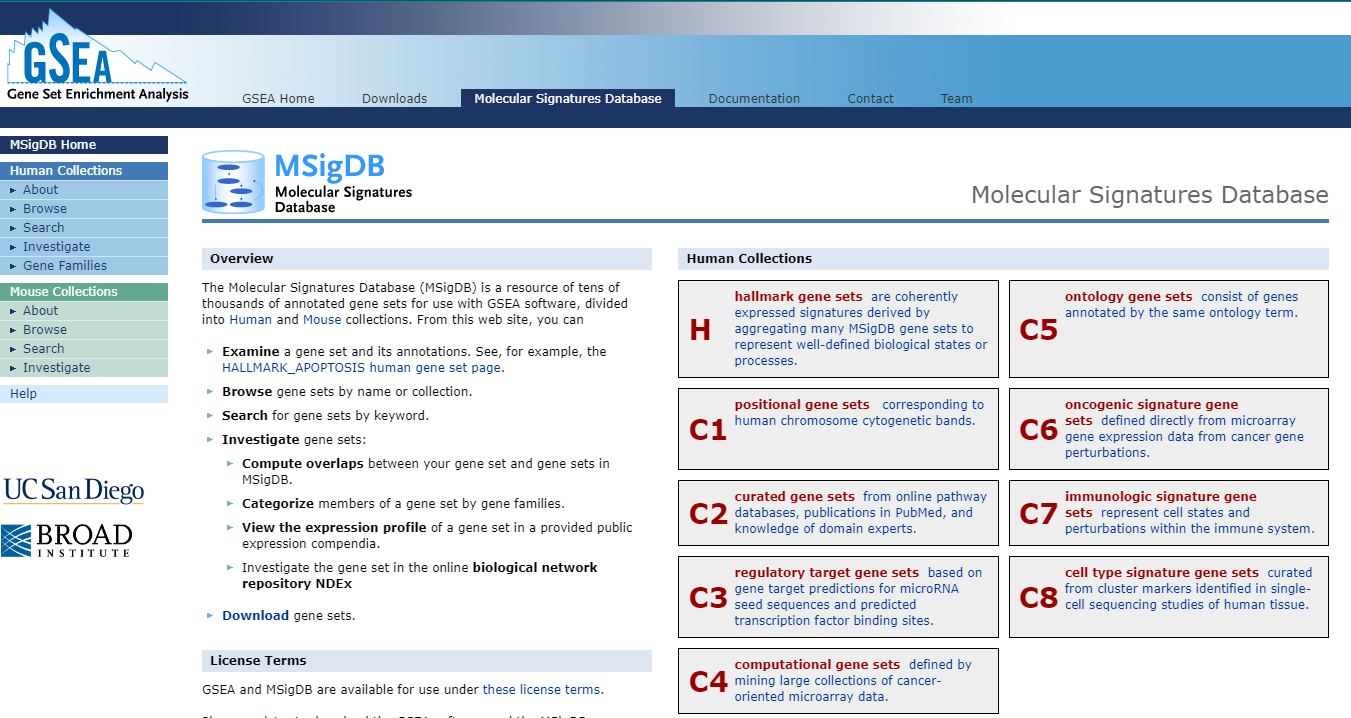
\includegraphics[width=0.95\linewidth]{./fig/gsea} 

}

\caption{Gene sets of MSigDb}\label{fig:unnamed-chunk-10}
\end{figure}

\begin{Shaded}
\begin{Highlighting}[]
\NormalTok{sig\_tme}\OtherTok{\textless{}{-}}\FunctionTok{calculate\_sig\_score}\NormalTok{(}\AttributeTok{pdata           =} \ConstantTok{NULL}\NormalTok{,}
                             \AttributeTok{eset            =}\NormalTok{ eset,}
                             \AttributeTok{signature       =}\NormalTok{ go\_bp,}
                             \AttributeTok{method          =} \StringTok{"ssgsea"}\NormalTok{,}
                             \AttributeTok{mini\_gene\_count =} \DecValTok{2}\NormalTok{)}
\end{Highlighting}
\end{Shaded}

\hypertarget{calculated-using-the-z-score-function.}{%
\section{Calculated using the z-score function.}\label{calculated-using-the-z-score-function.}}

\begin{Shaded}
\begin{Highlighting}[]
\NormalTok{sig\_tme}\OtherTok{\textless{}{-}}\FunctionTok{calculate\_sig\_score}\NormalTok{(}\AttributeTok{pdata           =} \ConstantTok{NULL}\NormalTok{,}
                             \AttributeTok{eset            =}\NormalTok{ eset,}
                             \AttributeTok{signature       =}\NormalTok{ signature\_collection,}
                             \AttributeTok{method          =} \StringTok{"zscore"}\NormalTok{,}
                             \AttributeTok{mini\_gene\_count =} \DecValTok{2}\NormalTok{)}
\end{Highlighting}
\end{Shaded}

\hypertarget{calculated-using-all-three-methods-at-the-same-time}{%
\section{Calculated using all three methods at the same time}\label{calculated-using-all-three-methods-at-the-same-time}}

\begin{Shaded}
\begin{Highlighting}[]
\NormalTok{sig\_tme}\OtherTok{\textless{}{-}}\FunctionTok{calculate\_sig\_score}\NormalTok{(}\AttributeTok{pdata           =} \ConstantTok{NULL}\NormalTok{,}
                             \AttributeTok{eset            =}\NormalTok{ eset,}
                             \AttributeTok{signature       =}\NormalTok{ signature\_collection,}
                             \AttributeTok{method          =} \StringTok{"integration"}\NormalTok{,}
                             \AttributeTok{mini\_gene\_count =} \DecValTok{2}\NormalTok{)}
\end{Highlighting}
\end{Shaded}

The same SIGNATURE in this case will be scored using all three methods simultaneously.

\begin{Shaded}
\begin{Highlighting}[]
\FunctionTok{colnames}\NormalTok{(sig\_tme)[}\FunctionTok{grep}\NormalTok{(}\FunctionTok{colnames}\NormalTok{(sig\_tme), }\AttributeTok{pattern =} \StringTok{"CD\_8\_T\_effector"}\NormalTok{)]}
\end{Highlighting}
\end{Shaded}

The \texttt{select\_method()} function allows the user to extract data using various methods.

\begin{Shaded}
\begin{Highlighting}[]
\NormalTok{sig\_tme\_pca }\OtherTok{\textless{}{-}} \FunctionTok{select\_method}\NormalTok{(}\AttributeTok{data =}\NormalTok{ sig\_tme, }\AttributeTok{method =} \StringTok{"pca"}\NormalTok{)}
\FunctionTok{colnames}\NormalTok{(sig\_tme\_pca)[}\FunctionTok{grep}\NormalTok{(}\FunctionTok{colnames}\NormalTok{(sig\_tme\_pca), }\AttributeTok{pattern =} \StringTok{"CD\_8\_T\_effector"}\NormalTok{)]}
\end{Highlighting}
\end{Shaded}

\hypertarget{how-to-customise-the-signature-gene-list-for-calculate_signature_score}{%
\section{\texorpdfstring{How to customise the signature gene list for \texttt{calculate\_signature\_score}}{How to customise the signature gene list for calculate\_signature\_score}}\label{how-to-customise-the-signature-gene-list-for-calculate_signature_score}}

\hypertarget{method-1-use-excel-for-storage-and-construction}{%
\subsection{Method-1: Use excel for storage and construction}\label{method-1-use-excel-for-storage-and-construction}}

Users can collect gene signatures using either an \texttt{Excel} or \texttt{CSV} file. The format should have the name of the signature in the first row, followed by the genes contained in each signature from the second row onwards. Once imported, the function \texttt{format\_signature} can be used to transform the data into a gene list of signatures required for \texttt{calculate\_signature\_score}. To import the file into R, users can use the functions read.csv or read\_excel. It is important to note here that the user needs to use the longest signature as a criterion and then replace all the vacant grids using NA, otherwise an error may be reported when reading into R.

Here we provide a sample data \texttt{sig\_excel}, please refer to this format to construct the required csv or excel files.

\begin{Shaded}
\begin{Highlighting}[]
\FunctionTok{data}\NormalTok{(}\StringTok{"sig\_excel"}\NormalTok{, }\AttributeTok{package =} \StringTok{"IOBR"}\NormalTok{)}
\NormalTok{sig }\OtherTok{\textless{}{-}} \FunctionTok{format\_signatures}\NormalTok{(sig\_excel)}
\FunctionTok{print}\NormalTok{(sig[}\DecValTok{1}\SpecialCharTok{:}\DecValTok{5}\NormalTok{])}
\end{Highlighting}
\end{Shaded}

\begin{verbatim}
## $Tcell_co_inhibitors
##  [1] "ADORA2A"  "BTLA"     "BTN2A2"   "BTN3A1"   "BTN3A2"   "BTNL2"   
##  [7] "C10orf54" "CSF1R"    "HAVCR2"   "IDO1"     "IL10"     "IL10RB"  
## [13] "KDR"      "KIR2DL1"  "SLAMF7"   "TGFB1"    "TIGIT"    "VRCN1"   
## [19] "VTCN1"    "CD247"    "CTLA4"    "CD160"    "CD244"    "CD274"   
## [25] "CD276"    "CD48"     "CD96"     "KIR2DL2"  "KIR2DL3"  "LAG3"    
## [31] "LAIR1"    "LGALS9"   "PVRL2"    "PDCD1"    "PDCD1LG2"
## 
## $Tcell_co_stimuiations
##  [1] "BTNL8"     "CD226"     "CD27"      "CD28"      "CD40"      "CD58"     
##  [7] "CD70"      "SLAMF1"    "TMIGD2"    "TNFRSF13B" "TNFRSF13C" "TNFRSF14" 
## [13] "TNFRSF4"   "TNFRSF8"   "TNFSF8"    "TNFSF9"    "ENTPD1"    "NT5E"     
## [19] "ICOS"      "TNFSF4"    "TNFSF15"   "CD80"      "CD86"      "EGFR"     
## [25] "HAVCR1"    "TNFSF18"   "ICOSLG"    "TNFSF13B"  "TNFRSF9"   "TNFSF13"  
## 
## $Tcell_function
## [1] "CD3E"  "CD4"   "CD8B"  "FOXP3" "GZMB"  "PRF1"  "TBX21" "IL2RA" "IKZF2"
## 
## $Tcell_checkpoint
##  [1] "CD274"    "CTLA4"    "LAG3"     "TIM3"     "TNFRSF9"  "TIGIT"   
##  [7] "CD226"    "CD7"      "GZMB"     "PRF1"     "TNFRSF18" "TNFRSF4" 
## [13] "HAVCR2"   "NLG1"     "CD4"      "CD8A"     "CD8B"     "FOXP3"   
## [19] "IL2"      "CXCL8"    "PDCD1"    "IFNG"    
## 
## $Teffctore_score
## [1] "CD8A"   "CXCL10" "CXCL9"  "GZMA"   "GZMB"   "IFNG"   "PRF1"   "TBX21"
\end{verbatim}

For simple structures or when the number of signatures to be added is relatively small, the following two methods can also be used.

\hypertarget{method-2-build-the-list-structure-directly}{%
\subsection{Method-2: Build the list structure directly}\label{method-2-build-the-list-structure-directly}}

\begin{Shaded}
\begin{Highlighting}[]
\NormalTok{sig }\OtherTok{\textless{}{-}} \FunctionTok{list}\NormalTok{(}\StringTok{"CD8"} \OtherTok{=} \FunctionTok{c}\NormalTok{(}\StringTok{"CD8A"}\NormalTok{,  }\StringTok{"CXCL10"}\NormalTok{, }\StringTok{"CXCL9"}\NormalTok{,  }\StringTok{"GZMA"}\NormalTok{,   }\StringTok{"GZMB"}\NormalTok{,   }\StringTok{"IFNG"}\NormalTok{,   }\StringTok{"PRF1"}\NormalTok{,   }\StringTok{"TBX21"}\NormalTok{),}
            \StringTok{"ICB"} \OtherTok{=} \FunctionTok{c}\NormalTok{(}\StringTok{"CD274"}\NormalTok{,   }\StringTok{"PDCD1LG2"}\NormalTok{, }\StringTok{"CTLA4"}\NormalTok{,    }\StringTok{"PDCD1"}\NormalTok{,    }\StringTok{"LAG3"}\NormalTok{,     }\StringTok{"HAVCR2"}\NormalTok{,   }\StringTok{"TIGIT"}\NormalTok{ ))}
\NormalTok{sig}
\end{Highlighting}
\end{Shaded}

\begin{verbatim}
## $CD8
## [1] "CD8A"   "CXCL10" "CXCL9"  "GZMA"   "GZMB"   "IFNG"   "PRF1"   "TBX21" 
## 
## $ICB
## [1] "CD274"    "PDCD1LG2" "CTLA4"    "PDCD1"    "LAG3"     "HAVCR2"   "TIGIT"
\end{verbatim}

\hypertarget{method3-add-the-new-signature-to-the-existing-gene-list}{%
\subsection{Method3: Add the new signature to the existing gene list}\label{method3-add-the-new-signature-to-the-existing-gene-list}}

\begin{Shaded}
\begin{Highlighting}[]
\NormalTok{sig}\OtherTok{\textless{}{-}}\NormalTok{ signature\_tumor}
\NormalTok{sig}\SpecialCharTok{$}\NormalTok{CD8 }\OtherTok{\textless{}{-}} \FunctionTok{c}\NormalTok{(}\StringTok{"CD8A"}\NormalTok{,  }\StringTok{"CXCL10"}\NormalTok{, }\StringTok{"CXCL9"}\NormalTok{,  }\StringTok{"GZMA"}\NormalTok{,   }\StringTok{"GZMB"}\NormalTok{,   }\StringTok{"IFNG"}\NormalTok{,   }\StringTok{"PRF1"}\NormalTok{,   }\StringTok{"TBX21"}\NormalTok{)}
\NormalTok{sig}
\end{Highlighting}
\end{Shaded}

\begin{verbatim}
## $Nature_metabolism_Hypoxia
##  [1] "ACOT7"  "SLC2A1" "ALDOA"  "CDKN3"  "ENO1"   "LDHA"   "MIF"    "MRPS17"
##  [9] "NDRG1"  "P4HA1"  "PGAM1"  "TPI1"   "TUBB6"  "VEGFA"  "ADM"   
## 
## $Winter_hypoxia_signature
## [1] "VEGF"  "GLUT1" "PDK-1" "EN01"  "HK2"   "CA9"   "AK3"   "CCNG2" "PFKB3"
## 
## $Hu_hypoxia_signature
##  [1] "FABP5"     "UCHL1"     "GAL"       "PLODDDIT4" "VEGF"      "ADM"      
##  [7] "ANGPTL4"   "NDRG1"     "NP"        "SLC16A3"   "C14ORF58"  "RRAGD"    
## 
## $Molecular_Cancer_m6A
##  [1] "METTL3"    "METTL14"   "RBM15"     "RBM15B"    "WTAP"      "KIAA1429" 
##  [7] "CBLL1"     "ZC3H13"    "ALKBH5"    "FTO"       "YTHDC1"    "YTHDC2"   
## [13] "YTHDF1"    "YTHDF2"    "YTHDF3"    "IGF2BP1"   "HNRNPA2B1" "HNRNPC"   
## [19] "FMR1"      "LRPPRC"    "ELAVL1"   
## 
## $MT_exosome
##  [1] "YWHAG"  "YWHAQ"  "CLTC"   "NCKAP1" "CFL1"   "ACTB"   "CCT4"   "RDX"   
##  [9] "GNA13"  "CTNNB1"
## 
## $SR_exosome
## [1] "HSP70" "HSP90" "CD9"   "CD63"  "CD81"  "CD82" 
## 
## $Positive_regulation_of_exosomal_secretion
##  [1] "ATP13A2" "CHMP2A"  "HGS"     "MYO5B"   "PDCD6IP" "RAB7"    "SDC1"   
##  [8] "SDC4"    "SDCBP"   "SMPD3"   "SNF8"    "STAM"    "TSG101"  "VPS4A"  
## 
## $Negative_regulation_of_exosomal_secretion
## [1] "VPS4B" "PRKN"  "RAB7" 
## 
## $Exosomal_secretion
## [1] "STEAP3" "TSG101" "RAB11A" "RAB27A" "COPS5" 
## 
## $Exosome_assembly
## [1] "CD34"    "PDCD6IP" "SDC1"    "SDC4"    "SDCBP"   "STAM"    "TSG101" 
## 
## $Extracellular_vesicle_biogenesis
##  [1] "ARRDC1"  "ARRDC4"  "ATP13A2" "CD34"    "CHMP2A"  "COPS5"   "HGS"    
##  [8] "MYO5B"   "PDCD6IP" "PRKN"    "RAB7"    "RAB11A"  "RAB27A"  "SDC1"   
## [15] "SDC4"    "SDCBP"   "SMPD3"   "SNF8"    "STAM"    "STEAP3"  "TSG101" 
## [22] "VPS4B"  
## 
## $MC_Review_Exosome1
##  [1] "TSG101"  "CD9"     "CD81"    "CD63"    "FLOT1"   "ITGB1"   "ITGA1"  
##  [8] "HSP70"   "AIP1"    "ALIX"    "PDCD6IP"
## 
## $MC_Review_Exosome2
##  [1] "RAB27A"  "RAB27B"  "PIKFYVE" "HRS"     "SYT7"    "CTTN"    "STAT3"  
##  [8] "PKM2"    "UNC13D"  "miR-155" "EGFR"    "RAS"     "EIF3C"   "LKB1"   
## [15] "STK11"  
## 
## $CMLS_Review_Exosome
##  [1] "HRS"      "STAM1"    "TSG101"   "CHMP4C"   "ALIX"     "VAT1"    
##  [7] "VPS4"     "CD9"      "CD82"     "CD63"     "LMP1"     "TSPAN8"  
## [13] "VAMP7"    "YKT6"     "PKM2"     "SNAP-23"  "RALA"     "RALB"    
## [19] "RAB2B"    "RAB5A"    "RAB9A"    "RAB7"     "RAB11"    "RAB27A"  
## [25] "RAB27B"   "RAB35"    "DGKA"     "PLD2"     "ARF6"     "ATG12"   
## [31] "ATG7"     "PIKFYVE"  "BST2"     "ATP6V0A4"
## 
## $Ferroptosis
##  [1] "ACSL4"      "AKR1C1-3"   "ALOXs"      "ATP5G3"     "CARS"      
##  [6] "CBS"        "CD44v"      "CHAC1"      "CISD1"      "CS"        
## [11] "DPP4"       "FANCD2"     "GCLC/GCLM"  "GLS2"       "GPX4"      
## [16] "GSS"        "HMGCR"      "HSPB1/5"    "KOD"        "LPCAT3"    
## [21] "MT1G"       "NCOA4"      "NFE2L2"     "PTGS2"      "RPL8"      
## [26] "SAT1"       "SLC7A11"    "SQS"        "TFRC"       "TP53"      
## [31] "TTC35/EMC2" "MESH1"     
## 
## $EV_Cell_2020
##  [1] "HSP90AB1" "HSP90AA1" "CD9"      "ALIX"     "FLOT1"    "FLOT2"   
##  [7] "TSG101"   "HSPA8"    "CD81"     "CD63"     "HBB"      "JCHAIN"  
## [13] "A2M"      "B2M"      "FN1"      "RAP1B"    "LGALS3BP" "GSN"     
## [19] "MSN"      "FLNA"     "ACTB"     "STOM"     "PRDX2"   
## 
## $CD8
## [1] "CD8A"   "CXCL10" "CXCL9"  "GZMA"   "GZMB"   "IFNG"   "PRF1"   "TBX21"
\end{verbatim}

\hypertarget{how-to-export-gene-signature}{%
\section{How to export gene signature}\label{how-to-export-gene-signature}}

Using the \texttt{output\_sig} function, user can export the signatures of the list structure to a csv file for other purposes. This step is exactly the reverse of \texttt{format\_signatures}.

\begin{Shaded}
\begin{Highlighting}[]
\NormalTok{sig }\OtherTok{\textless{}{-}} \FunctionTok{output\_sig}\NormalTok{(}\AttributeTok{signatures =}\NormalTok{ signature\_sc, }\AttributeTok{format =} \StringTok{"csv"}\NormalTok{, }\AttributeTok{file.name =} \StringTok{"sc\_signature"}\NormalTok{)}
\NormalTok{sig[}\DecValTok{1}\SpecialCharTok{:}\DecValTok{8}\NormalTok{, }\DecValTok{1}\SpecialCharTok{:}\DecValTok{5}\NormalTok{]}
\end{Highlighting}
\end{Shaded}

\begin{verbatim}
##   CD4_c0_Tcm CD4_c1_Treg CD4_c10_Tn_LEF1_ANKRD55 CD4_c11_Tisg CD4_c2_Tn
## 1      ANXA1       FOXP3                 ANKRD55        ISG15    NBEAL1
## 2       LMNA       IL2RA                    LEF1         IFI6      CCR7
## 3        VIM     TNFRSF4                    TCF7       IFI44L   GLTSCR2
## 4      KLRB1       TIGIT                   NOSIP          MX1      TCF7
## 5       IL7R      CARD16                    SELL        IFIT3    GNB2L1
## 6      ZFP36    TNFRSF18                   IL6ST        IFIT1      SELL
## 7    ZFP36L2        BATF                 LDLRAP1        RSAD2   C6orf48
## 8     GPR183       CTLA4                  RIPOR2        STAT1    TMEM66
\end{verbatim}

\hypertarget{references-1}{%
\section{References}\label{references-1}}

\textbf{ssgsea}: Barbie, D.A. et al (2009). Systematic RNA interference reveals that oncogenic KRAS-driven cancers require TBK1. Nature, 462(5):108-112.

\textbf{gsva}: Hänzelmann, S., Castelo, R. and Guinney, J. (2013). GSVA: Gene set variation analysis for microarray and RNA-Seq data. BMC Bioinformatics, 14(1):7.

\textbf{zscore}: Lee, E. et al (2008). Inferring pathway activity toward precise disease classification. PLoS Comp Biol, 4(11):e1000217.

\textbf{PCA method}: Mariathasan S, Turley SJ, Nickles D, et al.~TGFβ attenuates tumour response to PD-L1 blockade by contributing to exclusion of T cells. Nature. 2018 Feb 22;554(7693):544-548.

\textbf{MSigDB}:Dolgalev I (2022). msigdbr: MSigDB Gene Sets for Multiple Organisms in a Tidy Data Format. R package version 7.5.1. (\url{https://www.gsea-msigdb.org/gsea/msigdb/})

\hypertarget{tme-deconvolution}{%
\chapter{\texorpdfstring{\textbf{TME deconvolution}}{TME deconvolution}}\label{tme-deconvolution}}

This section demonstrates various algorithms for parsing the tumour microenvironment using data from the bulk transcriptome. We also describe how to construct the reference signature matrix for the popular SVR algorithm (CIBERSORT) from single-cell data.

\hypertarget{loading-packages-2}{%
\section{Loading packages}\label{loading-packages-2}}

Load the IOBR package in your R session after the installation is complete:

\begin{Shaded}
\begin{Highlighting}[]
\FunctionTok{library}\NormalTok{(IOBR)}
\FunctionTok{library}\NormalTok{(survminer)}
\FunctionTok{library}\NormalTok{(tidyverse)}
\end{Highlighting}
\end{Shaded}

\hypertarget{downloading-data-for-example-1}{%
\section{Downloading data for example}\label{downloading-data-for-example-1}}

Obtaining data set from GEO \href{https://pubmed.ncbi.nlm.nih.gov/25894828/}{Gastric cancer: GSE62254} using \texttt{GEOquery} R package.

\begin{Shaded}
\begin{Highlighting}[]
\ControlFlowTok{if}\NormalTok{ (}\SpecialCharTok{!}\FunctionTok{requireNamespace}\NormalTok{(}\StringTok{"GEOquery"}\NormalTok{, }\AttributeTok{quietly =} \ConstantTok{TRUE}\NormalTok{))  BiocManager}\SpecialCharTok{::}\FunctionTok{install}\NormalTok{(}\StringTok{"GEOquery"}\NormalTok{)}
\FunctionTok{library}\NormalTok{(}\StringTok{"GEOquery"}\NormalTok{)}
\CommentTok{\# }\AlertTok{NOTE}\CommentTok{: This process may take a few minutes which depends on the internet connection speed. Please wait for its completion.}
\NormalTok{eset\_geo }\OtherTok{\textless{}{-}} \FunctionTok{getGEO}\NormalTok{(}\AttributeTok{GEO =} \StringTok{"GSE62254"}\NormalTok{, }\AttributeTok{getGPL  =}\NormalTok{ F, }\AttributeTok{destdir =} \StringTok{"./"}\NormalTok{)}
\NormalTok{eset    }\OtherTok{\textless{}{-}}\NormalTok{ eset\_geo[[}\DecValTok{1}\NormalTok{]]}
\NormalTok{eset    }\OtherTok{\textless{}{-}} \FunctionTok{exprs}\NormalTok{(eset)}
\NormalTok{eset[}\DecValTok{1}\SpecialCharTok{:}\DecValTok{5}\NormalTok{, }\DecValTok{1}\SpecialCharTok{:}\DecValTok{5}\NormalTok{]}
\end{Highlighting}
\end{Shaded}

\begin{verbatim}
##           GSM1523727 GSM1523728 GSM1523729 GSM1523744 GSM1523745
## 1007_s_at  3.2176645  3.0624323  3.0279131   2.921683  2.8456013
## 1053_at    2.4050109  2.4394879  2.2442708   2.345916  2.4328582
## 117_at     1.4933412  1.8067380  1.5959665   1.839822  1.8326058
## 121_at     2.1965561  2.2812181  2.1865556   2.258599  2.1874363
## 1255_g_at  0.8698382  0.9502466  0.8125414   1.012860  0.9441993
\end{verbatim}

Annotation of genes in the expression matrix and removal of duplicate genes.

\begin{Shaded}
\begin{Highlighting}[]
\FunctionTok{library}\NormalTok{(IOBR)}

\CommentTok{\# Load the annotation file \textasciigrave{}anno\_hug133plus2\textasciigrave{} in IOBR.}
\FunctionTok{head}\NormalTok{(anno\_hug133plus2)}
\end{Highlighting}
\end{Shaded}

\begin{verbatim}
## # A tibble: 6 x 2
##   probe_id  symbol 
##   <fct>     <fct>  
## 1 1007_s_at MIR4640
## 2 1053_at   RFC2   
## 3 117_at    HSPA6  
## 4 121_at    PAX8   
## 5 1255_g_at GUCA1A 
## 6 1294_at   MIR5193
\end{verbatim}

\begin{Shaded}
\begin{Highlighting}[]
\CommentTok{\# Conduct gene annotation using \textasciigrave{}anno\_hug133plus2\textasciigrave{} file; If identical gene symbols exists, these genes would be ordered by the mean expression levels. The gene symbol with highest mean expression level is selected and remove others. }

\NormalTok{eset}\OtherTok{\textless{}{-}}\FunctionTok{anno\_eset}\NormalTok{(}\AttributeTok{eset       =}\NormalTok{ eset,}
                \AttributeTok{annotation =}\NormalTok{ anno\_hug133plus2,}
                \AttributeTok{symbol     =} \StringTok{"symbol"}\NormalTok{,}
                \AttributeTok{probe      =} \StringTok{"probe\_id"}\NormalTok{,}
                \AttributeTok{method     =} \StringTok{"mean"}\NormalTok{)}
\NormalTok{eset[}\DecValTok{1}\SpecialCharTok{:}\DecValTok{5}\NormalTok{, }\DecValTok{1}\SpecialCharTok{:}\DecValTok{3}\NormalTok{]}
\end{Highlighting}
\end{Shaded}

\begin{verbatim}
##              GSM1523727 GSM1523728 GSM1523729
## SH3KBP1        4.327974   4.316195   4.351425
## RPL41          4.246149   4.246808   4.257940
## EEF1A1         4.293762   4.291038   4.262199
## COX2           4.250288   4.283714   4.270508
## LOC101928826   4.219303   4.219670   4.213252
\end{verbatim}

\hypertarget{available-methods-to-decode-tme-contexture}{%
\section{Available Methods to Decode TME Contexture}\label{available-methods-to-decode-tme-contexture}}

\begin{Shaded}
\begin{Highlighting}[]
\NormalTok{tme\_deconvolution\_methods}
\end{Highlighting}
\end{Shaded}

\begin{verbatim}
##         MCPcounter               EPIC              xCell          CIBERSORT 
##       "mcpcounter"             "epic"            "xcell"        "cibersort" 
## CIBERSORT Absolute                IPS           ESTIMATE                SVR 
##    "cibersort_abs"              "ips"         "estimate"              "svr" 
##               lsei              TIMER          quanTIseq 
##             "lsei"            "timer"        "quantiseq"
\end{verbatim}

\begin{Shaded}
\begin{Highlighting}[]
\CommentTok{\# Return available parameter options of deconvolution methods}
\end{Highlighting}
\end{Shaded}

The input data is a matrix subseted from ESET of ACRG cohort, with genes in rows and samples in columns. The row name must be HGNC symbols and the column name must be sample names.

\begin{Shaded}
\begin{Highlighting}[]
\NormalTok{eset\_acrg }\OtherTok{\textless{}{-}}\NormalTok{ eset[, }\DecValTok{1}\SpecialCharTok{:}\DecValTok{50}\NormalTok{]}
\NormalTok{eset\_acrg[}\DecValTok{1}\SpecialCharTok{:}\DecValTok{5}\NormalTok{, }\DecValTok{1}\SpecialCharTok{:}\DecValTok{3}\NormalTok{]}
\end{Highlighting}
\end{Shaded}

\begin{verbatim}
##              GSM1523727 GSM1523728 GSM1523729
## SH3KBP1        4.327974   4.316195   4.351425
## RPL41          4.246149   4.246808   4.257940
## EEF1A1         4.293762   4.291038   4.262199
## COX2           4.250288   4.283714   4.270508
## LOC101928826   4.219303   4.219670   4.213252
\end{verbatim}

Check detail parameters of the function

\begin{Shaded}
\begin{Highlighting}[]
\CommentTok{\# help(deconvo\_tme)}
\end{Highlighting}
\end{Shaded}

\hypertarget{method-1-cibersort}{%
\section{Method 1: CIBERSORT}\label{method-1-cibersort}}

\begin{Shaded}
\begin{Highlighting}[]
\NormalTok{cibersort}\OtherTok{\textless{}{-}}\FunctionTok{deconvo\_tme}\NormalTok{(}\AttributeTok{eset =}\NormalTok{ eset\_acrg, }\AttributeTok{method =} \StringTok{"cibersort"}\NormalTok{, }\AttributeTok{arrays =} \ConstantTok{TRUE}\NormalTok{, }\AttributeTok{perm =} \DecValTok{100}\NormalTok{ )}
\end{Highlighting}
\end{Shaded}

\begin{verbatim}
## 
## >>> Running CIBERSORT
\end{verbatim}

\begin{Shaded}
\begin{Highlighting}[]
\CommentTok{\# head(cibersort)}
\NormalTok{res}\OtherTok{\textless{}{-}}\FunctionTok{cell\_bar\_plot}\NormalTok{(}\AttributeTok{input =}\NormalTok{ cibersort[}\DecValTok{1}\SpecialCharTok{:}\DecValTok{12}\NormalTok{,], }\AttributeTok{features =} \FunctionTok{colnames}\NormalTok{(cibersort)[}\DecValTok{3}\SpecialCharTok{:}\DecValTok{24}\NormalTok{], }\AttributeTok{title =} \StringTok{"CIBERSORT Cell Fraction"}\NormalTok{)}
\end{Highlighting}
\end{Shaded}

\begin{verbatim}
## There are seven categories you can choose: box, continue2, continue, random, heatmap, heatmap3, tidyheatmap
\end{verbatim}

\begin{verbatim}
## >>>>=== Palette option for random: 1: palette1; 2: palette2; 3: palette3;  4: palette4
\end{verbatim}

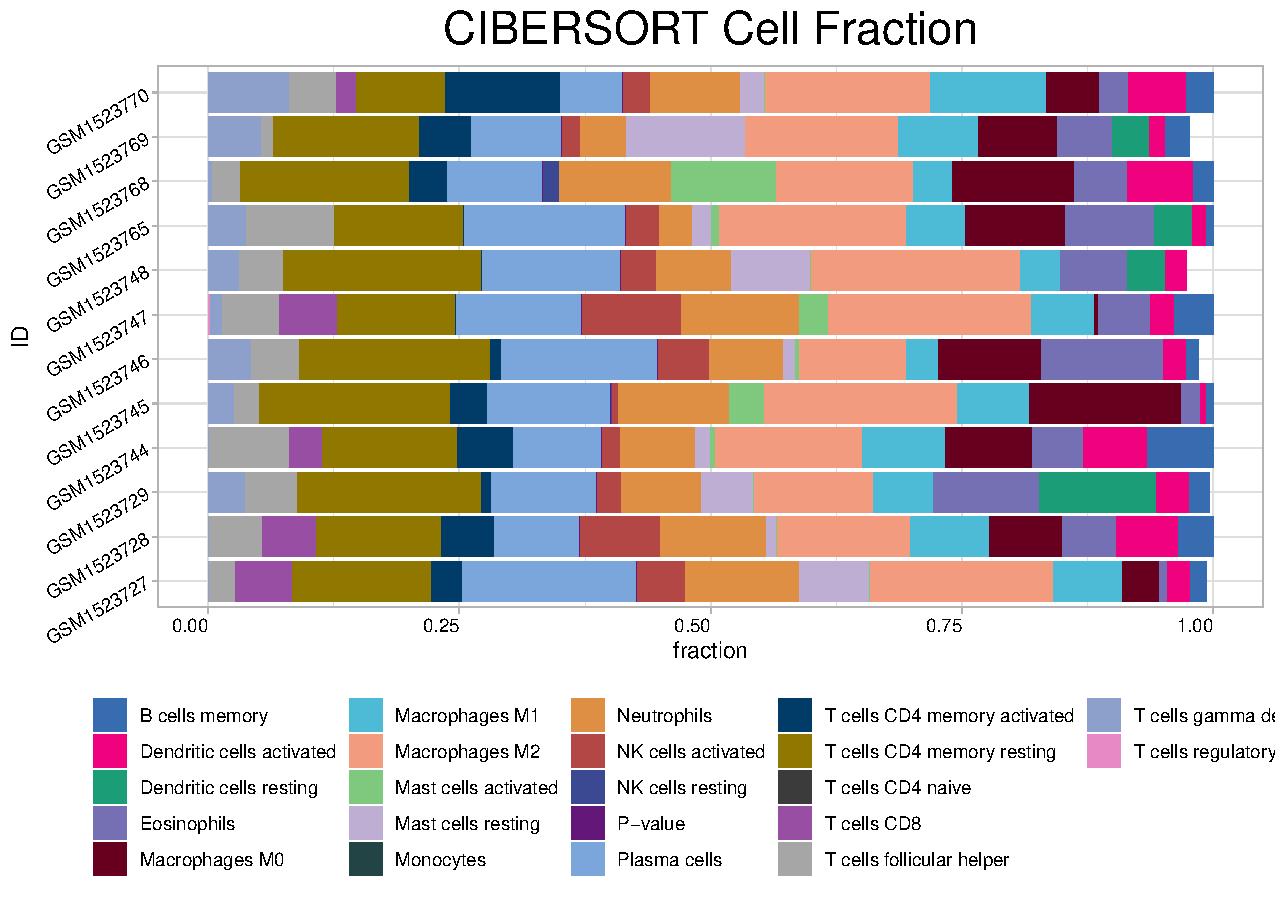
\includegraphics{tme-deconvolution_files/figure-latex/unnamed-chunk-7-1.pdf}

\hypertarget{method-2-epic}{%
\section{Method 2: EPIC}\label{method-2-epic}}

\begin{Shaded}
\begin{Highlighting}[]
\CommentTok{\# help(deconvo\_epic)}
\NormalTok{epic}\OtherTok{\textless{}{-}}\FunctionTok{deconvo\_tme}\NormalTok{(}\AttributeTok{eset =}\NormalTok{ eset\_acrg, }\AttributeTok{method =} \StringTok{"epic"}\NormalTok{, }\AttributeTok{arrays =} \ConstantTok{TRUE}\NormalTok{)}
\end{Highlighting}
\end{Shaded}

\begin{verbatim}
## 
## >>> Running EPIC
\end{verbatim}

\begin{verbatim}
## Warning in IOBR::EPIC(bulk = eset, reference = ref, mRNA_cell = NULL, scaleExprs = TRUE): The optimization didn't fully converge for some samples:
## GSM1523744; GSM1523746; GSM1523781; GSM1523786
##  - check fit.gof for the convergeCode and convergeMessage
\end{verbatim}

\begin{verbatim}
## Warning in IOBR::EPIC(bulk = eset, reference = ref, mRNA_cell = NULL,
## scaleExprs = TRUE): mRNA_cell value unknown for some cell types: CAFs,
## Endothelial - using the default value of 0.4 for these but this might bias the
## true cell proportions from all cell types.
\end{verbatim}

\begin{Shaded}
\begin{Highlighting}[]
\FunctionTok{head}\NormalTok{(epic)}
\end{Highlighting}
\end{Shaded}

\begin{verbatim}
## # A tibble: 6 x 9
##   ID      Bcells_EPIC CAFs_EPIC CD4_Tcells_EPIC CD8_Tcells_EPIC Endothelial_EPIC
##   <chr>         <dbl>     <dbl>           <dbl>           <dbl>            <dbl>
## 1 GSM152~      0.0292   0.00888           0.145          0.0756           0.0876
## 2 GSM152~      0.0293   0.0109            0.159          0.0745           0.0954
## 3 GSM152~      0.0308   0.0106            0.149          0.0732           0.0941
## 4 GSM152~      0.0273   0.0108            0.145          0.0704           0.0860
## 5 GSM152~      0.0280   0.0111            0.151          0.0707           0.0928
## 6 GSM152~      0.0320   0.00958           0.148          0.0716           0.0907
## # i 3 more variables: Macrophages_EPIC <dbl>, NKcells_EPIC <dbl>,
## #   otherCells_EPIC <dbl>
\end{verbatim}

\hypertarget{method-3-mcpcounter}{%
\section{Method 3: MCPcounter}\label{method-3-mcpcounter}}

\begin{Shaded}
\begin{Highlighting}[]
\NormalTok{mcp}\OtherTok{\textless{}{-}}\FunctionTok{deconvo\_tme}\NormalTok{(}\AttributeTok{eset =}\NormalTok{ eset\_acrg, }\AttributeTok{method =} \StringTok{"mcpcounter"}\NormalTok{)}
\end{Highlighting}
\end{Shaded}

\begin{verbatim}
## 
## >>> Running MCP-counter
\end{verbatim}

\begin{Shaded}
\begin{Highlighting}[]
\FunctionTok{head}\NormalTok{(mcp)}
\end{Highlighting}
\end{Shaded}

\begin{verbatim}
## # A tibble: 6 x 11
##   ID         T_cells_MCPcounter CD8_T_cells_MCPcounter Cytotoxic_lymphocytes_M~1
##   <chr>                   <dbl>                  <dbl>                     <dbl>
## 1 GSM1523727               1.47                  1.11                       1.33
## 2 GSM1523728               1.53                  1.05                       1.60
## 3 GSM1523729               1.47                  1.07                       1.37
## 4 GSM1523744               1.46                  1.02                       1.44
## 5 GSM1523745               1.51                  1.10                       1.49
## 6 GSM1523746               1.51                  0.992                      1.40
## # i abbreviated name: 1: Cytotoxic_lymphocytes_MCPcounter
## # i 7 more variables: B_lineage_MCPcounter <dbl>, NK_cells_MCPcounter <dbl>,
## #   Monocytic_lineage_MCPcounter <dbl>,
## #   Myeloid_dendritic_cells_MCPcounter <dbl>, Neutrophils_MCPcounter <dbl>,
## #   Endothelial_cells_MCPcounter <dbl>, Fibroblasts_MCPcounter <dbl>
\end{verbatim}

\hypertarget{method-4-xcell}{%
\section{Method 4: xCELL}\label{method-4-xcell}}

\begin{Shaded}
\begin{Highlighting}[]
\NormalTok{xcell}\OtherTok{\textless{}{-}}\FunctionTok{deconvo\_tme}\NormalTok{(}\AttributeTok{eset =}\NormalTok{ eset\_acrg, }\AttributeTok{method =} \StringTok{"xcell"}\NormalTok{, }\AttributeTok{arrays =} \ConstantTok{TRUE}\NormalTok{)}
\end{Highlighting}
\end{Shaded}

\begin{Shaded}
\begin{Highlighting}[]
\FunctionTok{head}\NormalTok{(xcell)}
\end{Highlighting}
\end{Shaded}

\begin{verbatim}
## # A tibble: 6 x 68
##   ID         aDC_xCell Adipocytes_xCell Astrocytes_xCell `B-cells_xCell`
##   <chr>          <dbl>            <dbl>            <dbl>           <dbl>
## 1 GSM1523727  4.78e-19          0.0250          0                 0     
## 2 GSM1523728  9.41e- 2          0.00433         7.70e- 3          0     
## 3 GSM1523729  1.02e- 1          0.0789          2.04e- 2          0     
## 4 GSM1523744  7.88e- 2          0.0538          4.82e-18          0.0126
## 5 GSM1523745  9.02e- 2          0.0136          1.93e- 2          0     
## 6 GSM1523746  3.40e- 2          0.0331          9.22e- 2          0     
## # i 63 more variables: Basophils_xCell <dbl>,
## #   `CD4+_memory_T-cells_xCell` <dbl>, `CD4+_naive_T-cells_xCell` <dbl>,
## #   `CD4+_T-cells_xCell` <dbl>, `CD4+_Tcm_xCell` <dbl>, `CD4+_Tem_xCell` <dbl>,
## #   `CD8+_naive_T-cells_xCell` <dbl>, `CD8+_T-cells_xCell` <dbl>,
## #   `CD8+_Tcm_xCell` <dbl>, `CD8+_Tem_xCell` <dbl>, cDC_xCell <dbl>,
## #   Chondrocytes_xCell <dbl>, `Class-switched_memory_B-cells_xCell` <dbl>,
## #   CLP_xCell <dbl>, CMP_xCell <dbl>, DC_xCell <dbl>, ...
\end{verbatim}

\hypertarget{method-5-estimate}{%
\section{Method 5: ESTIMATE}\label{method-5-estimate}}

\begin{Shaded}
\begin{Highlighting}[]
\NormalTok{estimate}\OtherTok{\textless{}{-}}\FunctionTok{deconvo\_tme}\NormalTok{(}\AttributeTok{eset =}\NormalTok{ eset\_acrg, }\AttributeTok{method =} \StringTok{"estimate"}\NormalTok{)}
\end{Highlighting}
\end{Shaded}

\begin{verbatim}
## [1] "Merged dataset includes 9940 genes (472 mismatched)."
## [1] "1 gene set: StromalSignature  overlap= 136"
## [1] "2 gene set: ImmuneSignature  overlap= 138"
\end{verbatim}

\begin{Shaded}
\begin{Highlighting}[]
\FunctionTok{head}\NormalTok{(estimate)}
\end{Highlighting}
\end{Shaded}

\begin{verbatim}
## # A tibble: 6 x 5
##   ID         StromalScore_estimate ImmuneScore_estimate ESTIMATEScore_estimate
##   <chr>                      <dbl>                <dbl>                  <dbl>
## 1 GSM1523727                -1250.                 268.                 -982. 
## 2 GSM1523728                  197.                1334.                 1531. 
## 3 GSM1523729                 -111.                 822.                  711. 
## 4 GSM1523744                 -119.                 662.                  544. 
## 5 GSM1523745                  324.                1015.                 1339. 
## 6 GSM1523746                 -594.                 621.                   27.0
## # i 1 more variable: TumorPurity_estimate <dbl>
\end{verbatim}

\hypertarget{method-6-timer}{%
\section{Method 6: TIMER}\label{method-6-timer}}

\begin{Shaded}
\begin{Highlighting}[]
\NormalTok{timer}\OtherTok{\textless{}{-}}\FunctionTok{deconvo\_tme}\NormalTok{(}\AttributeTok{eset =}\NormalTok{ eset\_acrg, }\AttributeTok{method =} \StringTok{"timer"}\NormalTok{, }\AttributeTok{group\_list =} \FunctionTok{rep}\NormalTok{(}\StringTok{"stad"}\NormalTok{,}\FunctionTok{dim}\NormalTok{(eset\_acrg)[}\DecValTok{2}\NormalTok{]))}
\end{Highlighting}
\end{Shaded}

\begin{verbatim}
## [1] "Outlier genes: AGR2 B2M COL1A2 COL3A1 COX2 CYAT1 EEF1A1 EIF1 FTH1 GKN1 HUWE1 IGK IGLC1 LIPF LOC101060363 LOC101928826 MIR8071-2 ND4 PABPC1 PABPC3 PGA4 RPL13AP5 RPL37 RPL37A RPL41 RPL7 RPS10 RPS16 RPS17 RPS18 RPS19 S100A6 S100A9 SH3KBP1 SNORD24 SNORD42A SNORD54 SNORD73A SPINK1 SPINK4 TFF1 UQCRFS1"
\end{verbatim}

\begin{Shaded}
\begin{Highlighting}[]
\FunctionTok{head}\NormalTok{(timer)}
\end{Highlighting}
\end{Shaded}

\begin{verbatim}
## # A tibble: 6 x 7
##   ID         B_cell_TIMER T_cell_CD4_TIMER T_cell_CD8_TIMER Neutrophil_TIMER
##   <chr>             <dbl>            <dbl>            <dbl>            <dbl>
## 1 GSM1523727        0.104            0.128            0.183            0.108
## 2 GSM1523728        0.103            0.130            0.192            0.118
## 3 GSM1523729        0.106            0.130            0.190            0.110
## 4 GSM1523744        0.101            0.126            0.187            0.111
## 5 GSM1523745        0.104            0.127            0.191            0.116
## 6 GSM1523746        0.105            0.129            0.192            0.111
## # i 2 more variables: Macrophage_TIMER <dbl>, DC_TIMER <dbl>
\end{verbatim}

\hypertarget{method-7-quantiseq}{%
\section{Method 7: quanTIseq}\label{method-7-quantiseq}}

\begin{Shaded}
\begin{Highlighting}[]
\NormalTok{quantiseq}\OtherTok{\textless{}{-}}\FunctionTok{deconvo\_tme}\NormalTok{(}\AttributeTok{eset =}\NormalTok{ eset\_acrg, }\AttributeTok{tumor =} \ConstantTok{TRUE}\NormalTok{, }\AttributeTok{arrays =} \ConstantTok{TRUE}\NormalTok{, }\AttributeTok{scale\_mrna =} \ConstantTok{TRUE}\NormalTok{, }\AttributeTok{method =} \StringTok{"quantiseq"}\NormalTok{)}
\end{Highlighting}
\end{Shaded}

\begin{verbatim}
## 
## Running quanTIseq deconvolution module
\end{verbatim}

\begin{verbatim}
## Gene expression normalization and re-annotation (arrays: TRUE)
\end{verbatim}

\begin{verbatim}
## Removing 17 genes with high expression in tumors
\end{verbatim}

\begin{verbatim}
## Signature genes found in data set: 152/153 (99.35%)
\end{verbatim}

\begin{verbatim}
## Mixture deconvolution (method: lsei)
\end{verbatim}

\begin{verbatim}
## Deconvolution sucessful!
\end{verbatim}

\begin{Shaded}
\begin{Highlighting}[]
\FunctionTok{head}\NormalTok{(quantiseq)}
\end{Highlighting}
\end{Shaded}

\begin{verbatim}
## # A tibble: 6 x 12
##   ID         B_cells_quantiseq Macrophages_M1_quantiseq Macrophages_M2_quantiseq
##   <chr>                  <dbl>                    <dbl>                    <dbl>
## 1 GSM1523727            0.0983                   0.0510                   0.0598
## 2 GSM1523728            0.0967                   0.0795                   0.0607
## 3 GSM1523729            0.102                    0.0450                   0.0758
## 4 GSM1523744            0.0954                   0.0725                   0.0579
## 5 GSM1523745            0.0991                   0.0669                   0.0613
## 6 GSM1523746            0.105                    0.0453                   0.0662
## # i 8 more variables: Monocytes_quantiseq <dbl>, Neutrophils_quantiseq <dbl>,
## #   NK_cells_quantiseq <dbl>, T_cells_CD4_quantiseq <dbl>,
## #   T_cells_CD8_quantiseq <dbl>, Tregs_quantiseq <dbl>,
## #   Dendritic_cells_quantiseq <dbl>, Other_quantiseq <dbl>
\end{verbatim}

\begin{Shaded}
\begin{Highlighting}[]
\NormalTok{res}\OtherTok{\textless{}{-}}\FunctionTok{cell\_bar\_plot}\NormalTok{(}\AttributeTok{input =}\NormalTok{ quantiseq[}\DecValTok{1}\SpecialCharTok{:}\DecValTok{12}\NormalTok{, ], }\AttributeTok{id =} \StringTok{"ID"}\NormalTok{, }\AttributeTok{features =} \FunctionTok{colnames}\NormalTok{(quantiseq)[}\DecValTok{2}\SpecialCharTok{:}\DecValTok{12}\NormalTok{], }\AttributeTok{title =} \StringTok{"quanTIseq Cell Fraction"}\NormalTok{)}
\end{Highlighting}
\end{Shaded}

\begin{verbatim}
## There are seven categories you can choose: box, continue2, continue, random, heatmap, heatmap3, tidyheatmap
\end{verbatim}

\begin{verbatim}
## >>>>=== Palette option for random: 1: palette1; 2: palette2; 3: palette3;  4: palette4
\end{verbatim}

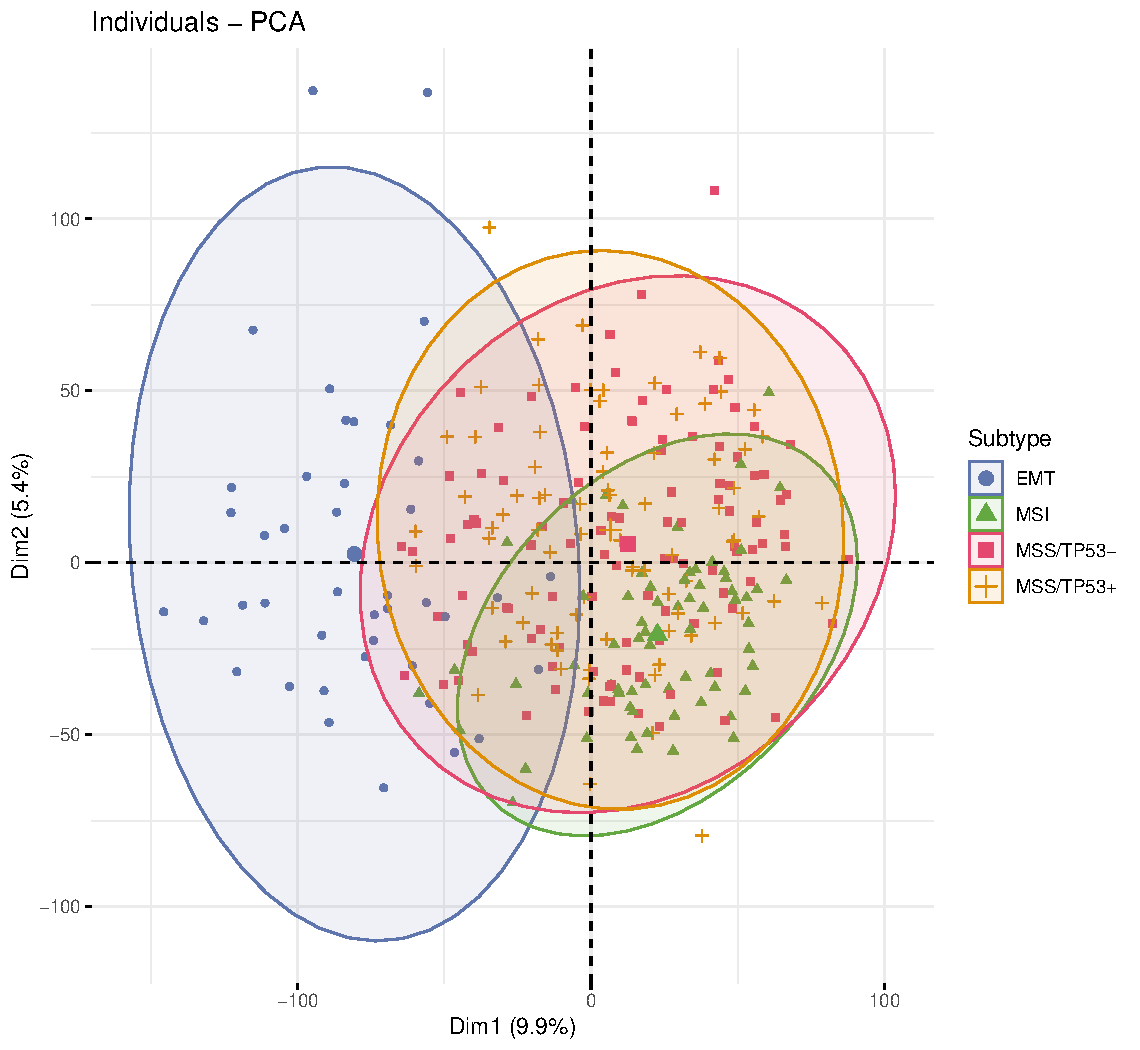
\includegraphics{tme-deconvolution_files/figure-latex/unnamed-chunk-14-1.pdf}

\hypertarget{method-8-ips}{%
\section{Method 8: IPS}\label{method-8-ips}}

\begin{Shaded}
\begin{Highlighting}[]
\NormalTok{ips}\OtherTok{\textless{}{-}}\FunctionTok{deconvo\_tme}\NormalTok{(}\AttributeTok{eset =}\NormalTok{ eset\_acrg, }\AttributeTok{method =} \StringTok{"ips"}\NormalTok{, }\AttributeTok{plot=} \ConstantTok{FALSE}\NormalTok{)}
\FunctionTok{head}\NormalTok{(ips)}
\end{Highlighting}
\end{Shaded}

\begin{verbatim}
## # A tibble: 6 x 7
##   ID         MHC_IPS EC_IPS SC_IPS  CP_IPS AZ_IPS IPS_IPS
##   <chr>        <dbl>  <dbl>  <dbl>   <dbl>  <dbl>   <dbl>
## 1 GSM1523727    2.25  0.404 -0.192  0.220    2.68       9
## 2 GSM1523728    2.37  0.608 -0.578 -0.234    2.17       7
## 3 GSM1523729    2.10  0.480 -0.322  0.0993   2.36       8
## 4 GSM1523744    2.12  0.535 -0.333  0.0132   2.34       8
## 5 GSM1523745    1.91  0.559 -0.479  0.0880   2.08       7
## 6 GSM1523746    1.94  0.458 -0.346  0.261    2.31       8
\end{verbatim}

\hypertarget{combination-of-above-deconvolution-results}{%
\section{Combination of above deconvolution results}\label{combination-of-above-deconvolution-results}}

\begin{Shaded}
\begin{Highlighting}[]
\NormalTok{tme\_combine}\OtherTok{\textless{}{-}}\NormalTok{cibersort }\SpecialCharTok{\%\textgreater{}\%} 
  \FunctionTok{inner\_join}\NormalTok{(.,mcp,}\AttributeTok{by       =} \StringTok{"ID"}\NormalTok{) }\SpecialCharTok{\%\textgreater{}\%} 
  \FunctionTok{inner\_join}\NormalTok{(.,xcell,}\AttributeTok{by     =} \StringTok{"ID"}\NormalTok{) }\SpecialCharTok{\%\textgreater{}\%}
  \FunctionTok{inner\_join}\NormalTok{(.,epic,}\AttributeTok{by      =} \StringTok{"ID"}\NormalTok{) }\SpecialCharTok{\%\textgreater{}\%} 
  \FunctionTok{inner\_join}\NormalTok{(.,estimate,}\AttributeTok{by  =} \StringTok{"ID"}\NormalTok{) }\SpecialCharTok{\%\textgreater{}\%} 
  \FunctionTok{inner\_join}\NormalTok{(.,timer,}\AttributeTok{by     =} \StringTok{"ID"}\NormalTok{) }\SpecialCharTok{\%\textgreater{}\%} 
  \FunctionTok{inner\_join}\NormalTok{(.,quantiseq,}\AttributeTok{by =} \StringTok{"ID"}\NormalTok{) }\SpecialCharTok{\%\textgreater{}\%} 
  \FunctionTok{inner\_join}\NormalTok{(.,ips,}\AttributeTok{by       =} \StringTok{"ID"}\NormalTok{)}
\FunctionTok{dim}\NormalTok{(tme\_combine)}
\end{Highlighting}
\end{Shaded}

\begin{verbatim}
## [1]  50 138
\end{verbatim}

\hypertarget{how-to-customise-the-signature-matrix-for-svr-and-lesi-algorithm}{%
\section{\texorpdfstring{How to customise the signature matrix for \texttt{SVR} and \texttt{lesi} algorithm}{How to customise the signature matrix for SVR and lesi algorithm}}\label{how-to-customise-the-signature-matrix-for-svr-and-lesi-algorithm}}

The recent surge in single-cell RNA sequencing has enabled us to identify novel microenvironmental cells, tumour microenvironmental characteristics, and tumour clonal signatures with high resolution. It is necessary to scrutinize, confirm and depict these features attained from high-dimensional single-cell information in bulk-seq with extended specimen sizes for clinical phenotyping. This is a demonstration using the results of 10X single-cell sequencing data of PBMC to construct gene signature matrix for \texttt{deconvo\_tme} function and estimate the abundance of these cell types in bulk transcriptome data.

Download PBMC dataset through: \url{https://cf.10xgenomics.com/samples/cell/pbmc3k/pbmc3k_filtered_gene_bc_matrices.tar.gz}

Initialize the Seurat object with the raw (non-normalized data).

\begin{Shaded}
\begin{Highlighting}[]
\FunctionTok{library}\NormalTok{(Seurat)}
\NormalTok{pbmc.data }\OtherTok{\textless{}{-}} \FunctionTok{Read10X}\NormalTok{(}\AttributeTok{data.dir =} \StringTok{"./pbmc3k\_filtered\_gene\_bc\_matrices/filtered\_gene\_bc\_matrices/hg19"}\NormalTok{)}
\NormalTok{pbmc }\OtherTok{\textless{}{-}} \FunctionTok{CreateSeuratObject}\NormalTok{(}\AttributeTok{counts =}\NormalTok{ pbmc.data, }\AttributeTok{project =} \StringTok{"pbmc3k"}\NormalTok{, }\AttributeTok{min.cells =} \DecValTok{3}\NormalTok{, }\AttributeTok{min.features =} \DecValTok{200}\NormalTok{)}
\end{Highlighting}
\end{Shaded}

Data prepare using Seurat's standard pipeline.

\begin{Shaded}
\begin{Highlighting}[]
\NormalTok{pbmc }\OtherTok{\textless{}{-}} \FunctionTok{FindVariableFeatures}\NormalTok{(pbmc, }\AttributeTok{selection.method =} \StringTok{"vst"}\NormalTok{, }\AttributeTok{nfeatures =} \DecValTok{2000}\NormalTok{, }\AttributeTok{verbose =} \ConstantTok{FALSE}\NormalTok{)}
\NormalTok{pbmc }\OtherTok{\textless{}{-}} \FunctionTok{NormalizeData}\NormalTok{(pbmc, }\AttributeTok{normalization.method =} \StringTok{"LogNormalize"}\NormalTok{, }\AttributeTok{scale.factor =} \DecValTok{10000}\NormalTok{, }\AttributeTok{verbose =} \ConstantTok{FALSE}\NormalTok{)}
\NormalTok{pbmc }\OtherTok{\textless{}{-}} \FunctionTok{ScaleData}\NormalTok{(pbmc, }\AttributeTok{features =}  \FunctionTok{rownames}\NormalTok{(pbmc), }\AttributeTok{verbose =} \ConstantTok{FALSE}\NormalTok{)}
\NormalTok{pbmc }\OtherTok{\textless{}{-}} \FunctionTok{RunPCA}\NormalTok{(pbmc, }\AttributeTok{features =} \FunctionTok{VariableFeatures}\NormalTok{(}\AttributeTok{object =}\NormalTok{ pbmc), }\AttributeTok{verbose =} \ConstantTok{FALSE}\NormalTok{)}
\NormalTok{pbmc }\OtherTok{\textless{}{-}} \FunctionTok{FindNeighbors}\NormalTok{(pbmc, }\AttributeTok{dims =} \DecValTok{1}\SpecialCharTok{:}\DecValTok{10}\NormalTok{, }\AttributeTok{verbose =} \ConstantTok{FALSE}\NormalTok{)}
\NormalTok{pbmc }\OtherTok{\textless{}{-}} \FunctionTok{FindClusters}\NormalTok{(pbmc, }\AttributeTok{resolution =} \FloatTok{0.5}\NormalTok{, }\AttributeTok{verbose =} \ConstantTok{FALSE}\NormalTok{)}
\CommentTok{\# Annotate cells according to seurat\textquotesingle{}s tutorials}
\CommentTok{\# https://satijalab.org/seurat/articles/pbmc3k\_tutorial}
\NormalTok{new.cluster.ids }\OtherTok{\textless{}{-}} \FunctionTok{c}\NormalTok{(}\StringTok{"Naive\_CD4\_T"}\NormalTok{, }\StringTok{"CD14\_Mono"}\NormalTok{, }\StringTok{"Memory\_CD4\_T"}\NormalTok{, }\StringTok{"Bcells"}\NormalTok{, }\StringTok{"CD8\_Tcell"}\NormalTok{, }\StringTok{"FCGR3A\_Mono"}\NormalTok{, }\StringTok{"NK"}\NormalTok{, }\StringTok{"DC"}\NormalTok{, }\StringTok{"Platelet"}\NormalTok{)}
\FunctionTok{names}\NormalTok{(new.cluster.ids) }\OtherTok{\textless{}{-}} \FunctionTok{levels}\NormalTok{(pbmc}\SpecialCharTok{$}\NormalTok{seurat\_clusters)}
\NormalTok{pbmc }\OtherTok{\textless{}{-}} \FunctionTok{RenameIdents}\NormalTok{(pbmc, new.cluster.ids)}
\NormalTok{pbmc}\SpecialCharTok{$}\NormalTok{celltype }\OtherTok{\textless{}{-}} \FunctionTok{Idents}\NormalTok{(pbmc)}
\end{Highlighting}
\end{Shaded}

Generate reference matrix using \texttt{generateRef\_seurat} function.

\begin{Shaded}
\begin{Highlighting}[]
\NormalTok{sm}\OtherTok{\textless{}{-}} \FunctionTok{generateRef\_seurat}\NormalTok{(}\AttributeTok{sce =}\NormalTok{ pbmc, }\AttributeTok{celltype =} \StringTok{"celltype"}\NormalTok{, }\AttributeTok{slot\_out =} \StringTok{"data"}\NormalTok{)}
\end{Highlighting}
\end{Shaded}

\begin{verbatim}
## >>>---Assay used to find markers: 
## [1] ">>>>> RNA"
## 
##       Bcells    CD14_Mono    CD8_Tcell           DC  FCGR3A_Mono Memory_CD4_T 
##          349          491          339           36          159          467 
##  Naive_CD4_T           NK     Platelet 
##          696          148           15 
## >>> Find markers of each celltype... 
## # A tibble: 450 x 7
## # Groups:   cluster [9]
##        p_val avg_log2FC pct.1 pct.2 p_val_adj cluster     gene 
##        <dbl>      <dbl> <dbl> <dbl>     <dbl> <fct>       <chr>
##  1 5.43e-142      0.681 0.999 0.994 7.45e-138 Naive_CD4_T RPS6 
##  2 5.65e-138      0.626 0.999 0.995 7.74e-134 Naive_CD4_T RPL32
##  3 5.62e-137      0.716 1     0.99  7.70e-133 Naive_CD4_T RPS12
##  4 1.90e-131      0.695 0.999 0.992 2.61e-127 Naive_CD4_T RPS27
##  5 2.36e-127      0.765 0.997 0.973 3.23e-123 Naive_CD4_T RPS25
##  6 3.96e-121      0.751 0.996 0.963 5.43e-117 Naive_CD4_T RPL31
##  7 2.91e-120      0.605 0.999 0.995 3.99e-116 Naive_CD4_T RPS14
##  8 1.74e-113      0.727 0.996 0.969 2.38e-109 Naive_CD4_T RPL9 
##  9 4.38e-110      0.590 0.999 0.993 6.01e-106 Naive_CD4_T RPS3 
## 10 6.80e-108      0.665 0.997 0.979 9.33e-104 Naive_CD4_T RPL30
## # i 440 more rows
## >>>-- Aggreating scRNAseq data...
## >>>-- `orig.ident` was set as group. User can define through parameter `celltype` ...
\end{verbatim}

Load the bulk RNA-seq data

\begin{Shaded}
\begin{Highlighting}[]
\FunctionTok{data}\NormalTok{(eset\_stad, }\AttributeTok{package =} \StringTok{"IOBR"}\NormalTok{)}
\NormalTok{eset }\OtherTok{\textless{}{-}} \FunctionTok{count2tpm}\NormalTok{(}\AttributeTok{countMat =}\NormalTok{ eset\_stad, }\AttributeTok{source =} \StringTok{"local"}\NormalTok{, }\AttributeTok{idType =} \StringTok{"ensembl"}\NormalTok{)}
\NormalTok{svr}\OtherTok{\textless{}{-}} \FunctionTok{deconvo\_tme}\NormalTok{(}\AttributeTok{eset =}\NormalTok{ eset, }\AttributeTok{reference  =}\NormalTok{ sm,  }\AttributeTok{method =} \StringTok{"svr"}\NormalTok{, }\AttributeTok{arrays  =} \ConstantTok{FALSE}\NormalTok{, }\AttributeTok{absolute.mode =} \ConstantTok{FALSE}\NormalTok{, }\AttributeTok{perm =} \DecValTok{100}\NormalTok{)}
\FunctionTok{head}\NormalTok{(svr)}
\end{Highlighting}
\end{Shaded}

\begin{verbatim}
## # A tibble: 6 x 13
##   ID           Naive_CD4_T_CIBERSORT CD14_Mono_CIBERSORT Memory_CD4_T_CIBERSORT
##   <chr>                        <dbl>               <dbl>                  <dbl>
## 1 TCGA-BR-6455                     0             0.143                    0.332
## 2 TCGA-BR-7196                     0             0.0862                   0.221
## 3 TCGA-BR-8371                     0             0.0642                   0.156
## 4 TCGA-BR-8380                     0             0.00125                  0.221
## 5 TCGA-BR-8592                     0             0.0621                   0.189
## 6 TCGA-BR-8686                     0             0.0411                   0.259
## # i 9 more variables: Bcells_CIBERSORT <dbl>, CD8_Tcell_CIBERSORT <dbl>,
## #   FCGR3A_Mono_CIBERSORT <dbl>, NK_CIBERSORT <dbl>, DC_CIBERSORT <dbl>,
## #   Platelet_CIBERSORT <dbl>, `P-value_CIBERSORT` <dbl>,
## #   Correlation_CIBERSORT <dbl>, RMSE_CIBERSORT <dbl>
\end{verbatim}

\begin{Shaded}
\begin{Highlighting}[]
\NormalTok{res}\OtherTok{\textless{}{-}}\FunctionTok{cell\_bar\_plot}\NormalTok{(}\AttributeTok{input =}\NormalTok{ svr, }\AttributeTok{features =} \FunctionTok{colnames}\NormalTok{(svr)[}\DecValTok{2}\SpecialCharTok{:}\DecValTok{10}\NormalTok{], }\AttributeTok{title =} \StringTok{"SVR Cell Fraction"}\NormalTok{)}
\end{Highlighting}
\end{Shaded}

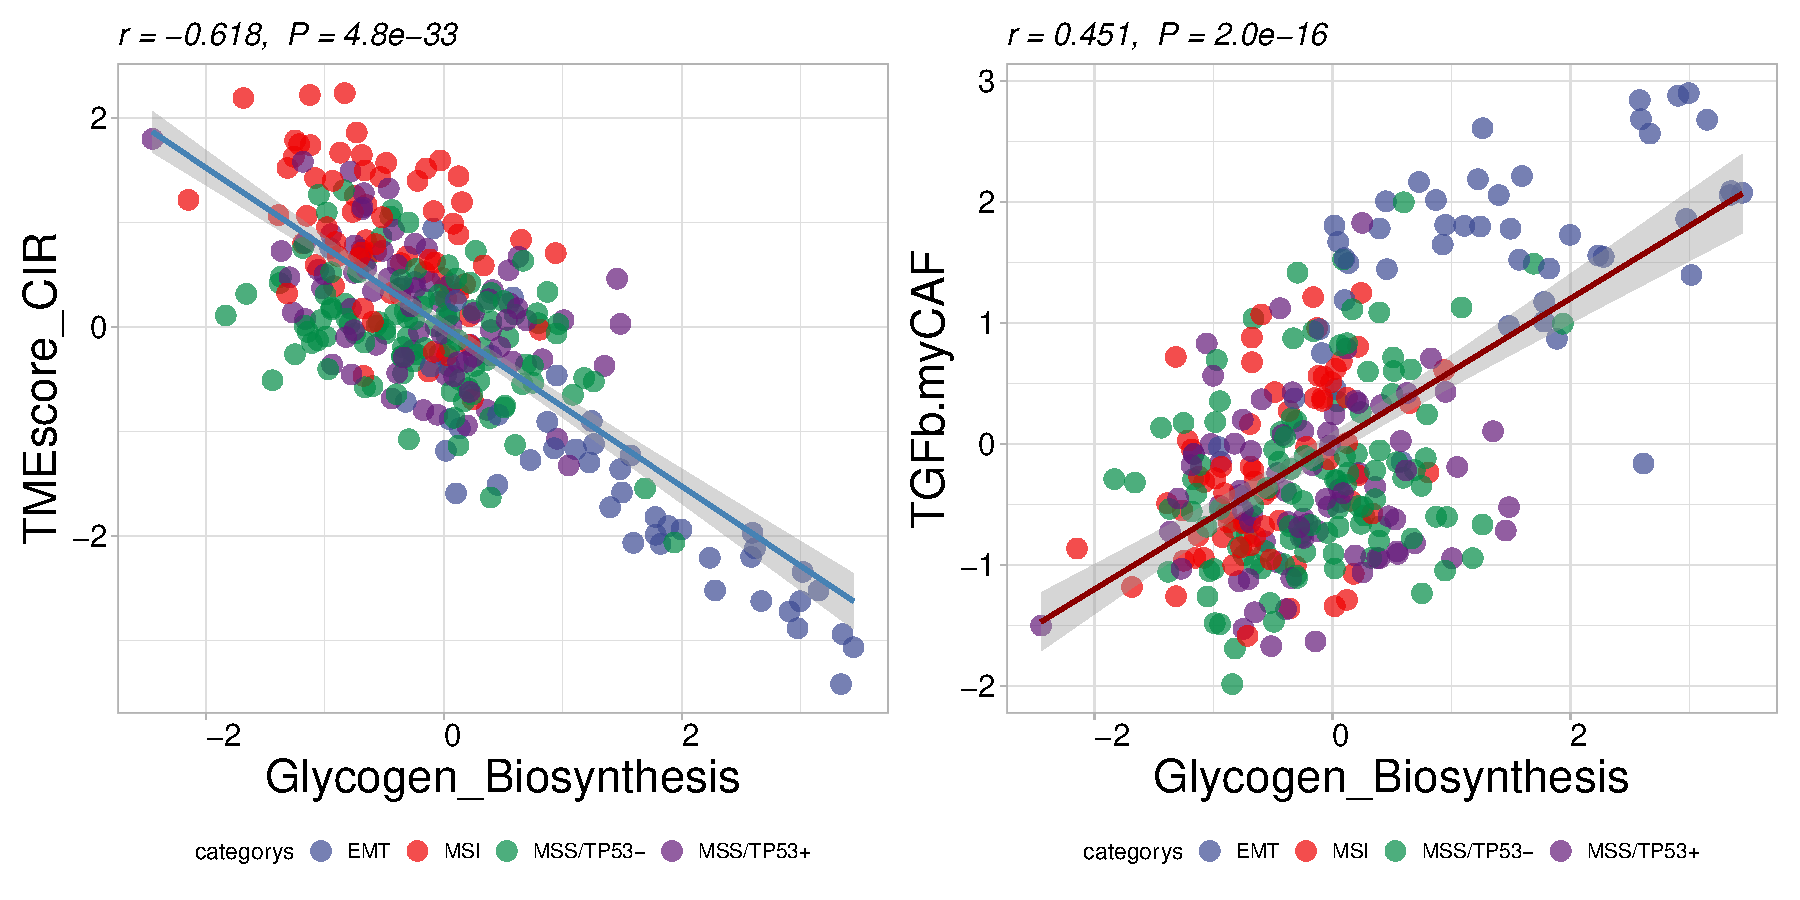
\includegraphics{tme-deconvolution_files/figure-latex/unnamed-chunk-21-1.pdf}

\hypertarget{references-2}{%
\section{References}\label{references-2}}

\textbf{If you use this package in your work, please cite both our package and the method(s) you are using.}

Citation and licenses of these deconvolution methods

\href{https://cibersort.stanford.edu/}{CIBERSORT}; free for non-commerical use only; Newman, A. M., Liu, C. L., Green, M. R., Gentles, A. J., Feng, W., Xu, Y., \ldots{} Alizadeh, A. A. (2015). Robust enumeration of cell subsets from tissue expression profiles. Nature Methods, 12(5), 453--457. \url{https://doi.org/10.1038/nmeth.3337};

\href{https://bioinformatics.mdanderson.org/public-software/estimate/}{ESTIMATE}; free (\href{https://bioinformatics.mdanderson.org/estimate/}{GPL2.0}); Vegesna R, Kim H, Torres-Garcia W, \ldots, Verhaak R. (2013). Inferring tumour purity and stromal and immune cell admixture from expression data. Nature Communications 4, 2612. \url{http://doi.org/10.1038/ncomms3612};

\href{http://icbi.at/software/quantiseq/doc/index.html}{quanTIseq}; free (\href{https://github.com/icbi-lab/immunedeconv/blob/master/LICENSE.md}{BSD}); Finotello, F., Mayer, C., Plattner, C., Laschober, G., Rieder, D., Hackl, H., \ldots, Sopper, S. (2019). Molecular and pharmacological modulators of the tumor immune contexture revealed by deconvolution of RNA-seq data. Genome medicine, 11(1), 34. \url{https://doi.org/10.1186/s13073-019-0638-6};

\href{http://cistrome.org/TIMER/}{TIMER}; free (\href{http://cistrome.org/TIMER/download.html}{GPL 2.0}); Li, B., Severson, E., Pignon, J.-C., Zhao, H., Li, T., Novak, J., \ldots{} Liu, X. S. (2016). Comprehensive analyses of tumor immunity: implications for cancer immunotherapy. Genome Biology, 17(1), 174. \url{https://doi.org/10.1186/s13059-016-1028-7};

\href{https://github.com/icbi-lab/Immunophenogram}{IPS}; free (\href{https://github.com/icbi-lab/Immunophenogram/blob/master/LICENSE}{BSD}); P. Charoentong et al., Pan-cancer Immunogenomic Analyses Reveal Genotype-Immunophenotype Relationships and Predictors of Response to Checkpoint Blockade. Cell Reports 18, 248-262 (2017). \url{https://doi.org/10.1016/j.celrep.2016.12.019};

\href{https://github.com/ebecht/MCPcounter}{MCPCounter}; free (\href{https://github.com/ebecht/MCPcounter/blob/master/Source/License}{GPL 3.0}); Becht, E., Giraldo, N. A., Lacroix, L., Buttard, B., Elarouci, N., Petitprez, F., \ldots{} de Reyniès, A. (2016). Estimating the population abundance of tissue-infiltrating immune and stromal cell populations using gene expression. Genome Biology, 17(1), 218. \url{https://doi.org/10.1186/s13059-016-1070-5};

\href{http://xcell.ucsf.edu/}{xCell}; free (\href{https://github.com/dviraran/xCell/blob/master/DESCRIPTION}{GPL 3.0}); Aran, D., Hu, Z., \& Butte, A. J. (2017). xCell: digitally portraying the tissue cellular heterogeneity landscape. Genome Biology, 18(1), 220. \url{https://doi.org/10.1186/s13059-017-1349-1};

\href{https://gfellerlab.shinyapps.io/EPIC_1-1/}{EPIC}; free for non-commercial use only (\href{https://github.com/GfellerLab/EPIC/blob/master/LICENSE}{Academic License}); Racle, J., de Jonge, K., Baumgaertner, P., Speiser, D. E., \& Gfeller, D. (2017). Simultaneous enumeration of cancer and immune cell types from bulk tumor gene expression data. ELife, 6, e26476. \url{https://doi.org/10.7554/eLife.26476};

\href{http://www.bioconductor.org/packages/release/bioc/html/GSVA.html}{GSVA} free (\href{https://github.com/rcastelo/GSVA}{GPL (\textgreater= 2)}) Hänzelmann S, Castelo R, Guinney J (2013). ``GSVA: gene set variation analysis for microarray and RNA-Seq data.'' BMC Bioinformatics, 14, 7. doi: 10.1186/1471-2105-14-7, \url{http://www.biomedcentral.com/1471-2105/14/7}

\hypertarget{signature-score-and-relevant-phenotypes}{%
\chapter{\texorpdfstring{\textbf{Signature Score and Relevant phenotypes}}{Signature Score and Relevant phenotypes}}\label{signature-score-and-relevant-phenotypes}}

\hypertarget{loading-packages-3}{%
\section{Loading packages}\label{loading-packages-3}}

Load the IOBR package in your R session after the installation is complete:

\begin{Shaded}
\begin{Highlighting}[]
\FunctionTok{library}\NormalTok{(IOBR)}
\FunctionTok{library}\NormalTok{(survminer)}
\FunctionTok{library}\NormalTok{(tidyverse)}
\end{Highlighting}
\end{Shaded}

\hypertarget{downloading-data-for-example-2}{%
\section{Downloading data for example}\label{downloading-data-for-example-2}}

Obtaining data set from GEO \href{https://pubmed.ncbi.nlm.nih.gov/25894828/}{Gastric cancer: GSE62254} using \texttt{GEOquery} R package.

\begin{Shaded}
\begin{Highlighting}[]
\ControlFlowTok{if}\NormalTok{ (}\SpecialCharTok{!}\FunctionTok{requireNamespace}\NormalTok{(}\StringTok{"GEOquery"}\NormalTok{, }\AttributeTok{quietly =} \ConstantTok{TRUE}\NormalTok{))  BiocManager}\SpecialCharTok{::}\FunctionTok{install}\NormalTok{(}\StringTok{"GEOquery"}\NormalTok{)}
\FunctionTok{library}\NormalTok{(}\StringTok{"GEOquery"}\NormalTok{)}
\CommentTok{\# }\AlertTok{NOTE}\CommentTok{: This process may take a few minutes which depends on the internet connection speed. Please wait for its completion.}
\NormalTok{eset\_geo }\OtherTok{\textless{}{-}} \FunctionTok{getGEO}\NormalTok{(}\AttributeTok{GEO =} \StringTok{"GSE62254"}\NormalTok{, }\AttributeTok{getGPL  =}\NormalTok{ F, }\AttributeTok{destdir =} \StringTok{"./"}\NormalTok{)}
\NormalTok{eset    }\OtherTok{\textless{}{-}}\NormalTok{ eset\_geo[[}\DecValTok{1}\NormalTok{]]}
\NormalTok{eset    }\OtherTok{\textless{}{-}} \FunctionTok{exprs}\NormalTok{(eset)}
\NormalTok{eset[}\DecValTok{1}\SpecialCharTok{:}\DecValTok{5}\NormalTok{,}\DecValTok{1}\SpecialCharTok{:}\DecValTok{5}\NormalTok{]}
\end{Highlighting}
\end{Shaded}

\begin{verbatim}
##           GSM1523727 GSM1523728 GSM1523729 GSM1523744 GSM1523745
## 1007_s_at  3.2176645  3.0624323  3.0279131   2.921683  2.8456013
## 1053_at    2.4050109  2.4394879  2.2442708   2.345916  2.4328582
## 117_at     1.4933412  1.8067380  1.5959665   1.839822  1.8326058
## 121_at     2.1965561  2.2812181  2.1865556   2.258599  2.1874363
## 1255_g_at  0.8698382  0.9502466  0.8125414   1.012860  0.9441993
\end{verbatim}

\hypertarget{gene-annotation-1}{%
\section{Gene Annotation}\label{gene-annotation-1}}

Annotation of genes in the expression matrix and removal of duplicate genes.

\begin{Shaded}
\begin{Highlighting}[]
\CommentTok{\# Load the annotation file \textasciigrave{}anno\_hug133plus2\textasciigrave{} in IOBR.}
\FunctionTok{head}\NormalTok{(anno\_hug133plus2)}
\end{Highlighting}
\end{Shaded}

\begin{verbatim}
## # A tibble: 6 x 2
##   probe_id  symbol 
##   <fct>     <fct>  
## 1 1007_s_at MIR4640
## 2 1053_at   RFC2   
## 3 117_at    HSPA6  
## 4 121_at    PAX8   
## 5 1255_g_at GUCA1A 
## 6 1294_at   MIR5193
\end{verbatim}

\begin{Shaded}
\begin{Highlighting}[]
\CommentTok{\# Conduct gene annotation using \textasciigrave{}anno\_hug133plus2\textasciigrave{} file; If identical gene symbols exists, these genes would be ordered by the mean expression levels. The gene symbol with highest mean expression level is selected and remove others. }

\NormalTok{eset}\OtherTok{\textless{}{-}}\FunctionTok{anno\_eset}\NormalTok{(}\AttributeTok{eset       =}\NormalTok{ eset,}
                \AttributeTok{annotation =}\NormalTok{ anno\_hug133plus2,}
                \AttributeTok{symbol     =} \StringTok{"symbol"}\NormalTok{,}
                \AttributeTok{probe      =} \StringTok{"probe\_id"}\NormalTok{,}
                \AttributeTok{method     =} \StringTok{"mean"}\NormalTok{)}
\NormalTok{eset[}\DecValTok{1}\SpecialCharTok{:}\DecValTok{5}\NormalTok{, }\DecValTok{1}\SpecialCharTok{:}\DecValTok{3}\NormalTok{]}
\end{Highlighting}
\end{Shaded}

\begin{verbatim}
##              GSM1523727 GSM1523728 GSM1523729
## SH3KBP1        4.327974   4.316195   4.351425
## RPL41          4.246149   4.246808   4.257940
## EEF1A1         4.293762   4.291038   4.262199
## COX2           4.250288   4.283714   4.270508
## LOC101928826   4.219303   4.219670   4.213252
\end{verbatim}

\hypertarget{estimation-of-signatures}{%
\section{Estimation of signatures}\label{estimation-of-signatures}}

\begin{Shaded}
\begin{Highlighting}[]
\NormalTok{sig\_tme}\OtherTok{\textless{}{-}}\FunctionTok{calculate\_sig\_score}\NormalTok{(}\AttributeTok{pdata           =} \ConstantTok{NULL}\NormalTok{,}
                             \AttributeTok{eset            =}\NormalTok{ eset,}
                             \AttributeTok{signature       =}\NormalTok{ signature\_collection,}
                             \AttributeTok{method          =} \StringTok{"pca"}\NormalTok{,}
                             \AttributeTok{mini\_gene\_count =} \DecValTok{2}\NormalTok{)}

\NormalTok{sig\_tme }\OtherTok{\textless{}{-}} \FunctionTok{t}\NormalTok{(}\FunctionTok{column\_to\_rownames}\NormalTok{(sig\_tme, }\AttributeTok{var =} \StringTok{"ID"}\NormalTok{))}
\NormalTok{sig\_tme[}\DecValTok{1}\SpecialCharTok{:}\DecValTok{5}\NormalTok{, }\DecValTok{1}\SpecialCharTok{:}\DecValTok{3}\NormalTok{]}
\end{Highlighting}
\end{Shaded}

\begin{verbatim}
##                   GSM1523727 GSM1523728 GSM1523729
## CD_8_T_effector   -2.5513794  0.7789141 -2.1770675
## DDR               -0.8747614  0.7425162 -1.3272054
## APM                1.1098368  2.1988688 -0.9516419
## Immune_Checkpoint -2.3701787  0.9455120 -1.4844104
## CellCycle_Reg      0.1063358  0.7583302 -0.3649795
\end{verbatim}

\hypertarget{combining-score-data-and-phenotype-data}{%
\section{Combining score data and phenotype data}\label{combining-score-data-and-phenotype-data}}

\begin{Shaded}
\begin{Highlighting}[]
\FunctionTok{data}\NormalTok{(}\StringTok{"pdata\_acrg"}\NormalTok{, }\AttributeTok{package =} \StringTok{"IOBR"}\NormalTok{)}
\FunctionTok{head}\NormalTok{(pdata\_acrg)}
\end{Highlighting}
\end{Shaded}

\begin{verbatim}
##            ID ProjectID  Technology       platform Gender Age RFS_time
## 71 GSM1523727  GSE62254 Affymetrix  HG-U133_Plus_2      M  67     3.97
## 72 GSM1523728  GSE62254 Affymetrix  HG-U133_Plus_2      F  68     4.03
## 73 GSM1523729  GSE62254 Affymetrix  HG-U133_Plus_2      F  42    74.97
## 74 GSM1523744  GSE62254 Affymetrix  HG-U133_Plus_2      M  69    89.77
## 75 GSM1523745  GSE62254 Affymetrix  HG-U133_Plus_2      M  68    84.60
## 76 GSM1523746  GSE62254 Affymetrix  HG-U133_Plus_2      M  56     5.77
##    RFS_status OS_time OS_status     Lauren Differtiation AJCC_Stage_confuse
## 71         NA   88.73         0 Intestinal            MD                  2
## 72         NA   88.23         0 Intestinal            PD                  2
## 73          0   88.23         0    Diffuse            PD                  2
## 74          0  105.70         0    Diffuse            PD                  2
## 75          0  105.53         0    Diffuse            PD                  3
## 76          1   25.50         1      Mixed            PD                  2
##    T_stage N_stage M_stage Lymph_node_examined Positive_lymph_nodes
## 71       2       1       0                  20                    3
## 72       2       1       0                  40                    1
## 73       2       1       0                  21                    1
## 74       2       1       0                  24                    3
## 75       3       2       0                  52                   11
## 76       2       1       0                  22                    5
##    Revisedlocation MSI EBV Hpylori   Subtype TP53mutated B.cells.naive
## 71            Body   1   0      NA       MSI           0   0.006611704
## 72            Body   1  NA      NA       MSI           0   0.000000000
## 73          Antrum   0   0       0 MSS/TP53+           1   0.003306927
## 74          Antrum   1   0       1       MSI           0   0.000000000
## 75          Antrum   0   0      NA MSS/TP53-           0   0.000000000
## 76          Antrum   0   0       0 MSS/TP53-           0   0.013619480
##    B.cells.memory Plasma.cells T.cells.CD8 T.cells.CD4.naive
## 71    0.014570868   0.17555729  0.05712737                 0
## 72    0.036202099   0.08523233  0.05336971                 0
## 73    0.020935673   0.10489546  0.00000000                 0
## 74    0.072648177   0.08755997  0.03465107                 0
## 75    0.009798381   0.12251030  0.00000000                 0
## 76    0.012784581   0.15602714  0.00000000                 0
##    T.cells.CD4.memory.resting T.cells.CD4.memory.activated
## 71                  0.1439895                  0.025159835
## 72                  0.1250515                  0.049617381
## 73                  0.1849220                  0.008407981
## 74                  0.1396439                  0.055268600
## 75                  0.1916398                  0.036578672
## 76                  0.1905921                  0.008992440
##    T.cells.follicular.helper T.cells.regulatory..Tregs. T.cells.gamma.delta
## 71                0.02453957                          0          0.00000000
## 72                0.05318251                          0          0.00000000
## 73                0.05098080                          0          0.03714459
## 74                0.07825130                          0          0.00000000
## 75                0.02223859                          0          0.02657259
## 76                0.04740728                          0          0.04283296
##    NK.cells.resting NK.cells.activated Monocytes Macrophages.M0 Macrophages.M1
## 71      0.000000000        0.049325657         0     0.03865693     0.06910287
## 72      0.000000000        0.081481924         0     0.07370723     0.08016443
## 73      0.000000000        0.025252673         0     0.00000000     0.06161940
## 74      0.000000000        0.016121853         0     0.08866391     0.08173804
## 75      0.001738259        0.006267907         0     0.15255902     0.07161270
## 76      0.000000000        0.052117471         0     0.10298038     0.03246627
##    Macrophages.M2 Dendritic.cells.resting Dendritic.cells.activated
## 71      0.1829208               0.0000000               0.022904531
## 72      0.1320919               0.0000000               0.060491149
## 73      0.1170839               0.1171129               0.032385282
## 74      0.1441202               0.0000000               0.060937005
## 75      0.1919279               0.0000000               0.006087801
## 76      0.1093805               0.0000000               0.023914527
##    Mast.cells.resting Mast.cells.activated Eosinophils Neutrophils.x P.value
## 71        0.069286038          0.000000000 0.006315889    0.11393115       0
## 72        0.003322764          0.005197745 0.056141443    0.10474585       0
## 73        0.052571970          0.000000000 0.104493538    0.07888690       0
## 74        0.012494201          0.006833953 0.050435095    0.07063272       0
## 75        0.000000000          0.033928747 0.017164438    0.10937487       0
## 76        0.014373257          0.002764802 0.115772442    0.07397439       0
##    Pearson.Correlation      RMSE    T.cells CD8.T.cells Cytotoxic.lymphocytes
## 71           0.3359926 0.9415173 -0.9275804   0.8492914            -1.1005262
## 72           0.4793134 0.8827802 -0.5306279  -0.2017907             0.1858499
## 73           0.3638005 0.9308186 -0.9566316   0.2411951            -0.8800338
## 74           0.3569989 0.9332100 -1.0464552  -0.5771205            -0.5619472
## 75           0.4226987 0.9062522 -0.6796120   0.6670229            -0.3361456
## 76           0.4113346 0.9112588 -0.6978480  -1.1110102            -0.7631710
##        NK.cells   B.lineage Monocytic.lineage Myeloid.dendritic.cells
## 71 -0.083623737 -0.54974243       -1.40389061              -0.7589211
## 72  0.156167025 -0.33750363       -0.03696397              -0.6393975
## 73  0.003538847  0.01597566       -0.67105808               0.7452174
## 74 -0.010774923 -0.56740438        0.06877240              -0.2511140
## 75 -0.028429092 -0.73180429        0.21574792              -0.1165082
## 76  0.466964699  0.15583392       -0.97524359              -0.7448360
##    Neutrophils.y Endothelial.cells Fibroblasts StromalScore ImmuneScore
## 71    -0.9527759       -1.42753593 -1.22754105   -1.8047694  -1.3347047
## 72     0.5640500       -0.17320689  0.41586717    0.1825225   0.1950604
## 73    -0.3415288       -0.25784297  0.04110246   -0.1863425  -0.4960305
## 74    -1.2984378       -1.05394707  0.00743277   -0.2731398  -0.7950682
## 75     0.4227674        0.03025664  0.32245183    0.3165798  -0.2416774
## 76    -0.4411653       -0.29582293 -0.68833740   -0.9119449  -0.8475150
##    ESTIMATEScore TumorPurity ProjectID2   TMEscoreA    TMEscoreB    TMEscore
## 71   -1.70632719   1.1687573   GSE62254 -1.06110812 -1.270222413  0.60585688
## 72    0.20292720          NA   GSE62254  1.14698153 -0.333585646  0.73717229
## 73   -0.35721073  -1.3859061   GSE62254 -0.89026369 -0.007906066 -0.35452887
## 74   -0.55795758  -0.9855180   GSE62254 -0.01116022 -0.984841623  0.79880007
## 75    0.05885805          NA   GSE62254 -0.27102383 -0.017592784 -0.09554256
## 76   -0.94967710  -0.2162267   GSE62254 -0.94526260  0.161818627 -0.51527214
##    TMEscore_binary
## 71             Low
## 72            High
## 73             Low
## 74            High
## 75             Low
## 76             Low
\end{verbatim}

\begin{Shaded}
\begin{Highlighting}[]
\NormalTok{input }\OtherTok{\textless{}{-}} \FunctionTok{combine\_pd\_eset}\NormalTok{(}\AttributeTok{eset =}\NormalTok{ sig\_tme, }\AttributeTok{pdata =}\NormalTok{ pdata\_acrg, }\AttributeTok{scale =}\NormalTok{ T)}
\end{Highlighting}
\end{Shaded}

\hypertarget{identifying-features-associated-with-survival}{%
\section{Identifying features associated with survival}\label{identifying-features-associated-with-survival}}

\begin{Shaded}
\begin{Highlighting}[]
\NormalTok{res}\OtherTok{\textless{}{-}} \FunctionTok{batch\_surv}\NormalTok{(}\AttributeTok{pdata    =}\NormalTok{ input,}
                 \AttributeTok{time     =} \StringTok{"OS\_time"}\NormalTok{, }
                 \AttributeTok{status   =} \StringTok{"OS\_status"}\NormalTok{, }
                 \AttributeTok{variable =} \FunctionTok{colnames}\NormalTok{(input)[}\DecValTok{69}\SpecialCharTok{:}\FunctionTok{ncol}\NormalTok{(input)])}
\FunctionTok{head}\NormalTok{(res)}
\end{Highlighting}
\end{Shaded}

\begin{verbatim}
## # A tibble: 6 x 5
##   ID                           P    HR CI_low_0.95 CI_up_0.95
##   <chr>                    <dbl> <dbl>       <dbl>      <dbl>
## 1 Folate_biosynthesis   1.00e-10 0.579       0.490      0.683
## 2 TMEscore_CIR          1.32e- 9 0.640       0.554      0.739
## 3 Glycogen_Biosynthesis 3.24e- 9 1.52        1.32       1.74 
## 4 Pan_F_TBRs            6.33e- 9 1.55        1.34       1.80 
## 5 TMEscoreB_CIR         7.17e- 9 1.52        1.32       1.75 
## 6 TMEscore_plus         8.08e- 9 0.638       0.547      0.743
\end{verbatim}

Use forest plots \texttt{sig\_forest} to show the most relevant variables to overall survival

\begin{Shaded}
\begin{Highlighting}[]
\NormalTok{res}\OtherTok{\textless{}{-}}\NormalTok{ res[}\FunctionTok{nchar}\NormalTok{(res}\SpecialCharTok{$}\NormalTok{ID)}\SpecialCharTok{\textless{}=}\DecValTok{28}\NormalTok{, ]}
\NormalTok{p1}\OtherTok{\textless{}{-}} \FunctionTok{sig\_forest}\NormalTok{(res, }\AttributeTok{signature =} \StringTok{"ID"}\NormalTok{, }\AttributeTok{n =} \DecValTok{20}\NormalTok{)}
\end{Highlighting}
\end{Shaded}

\begin{center}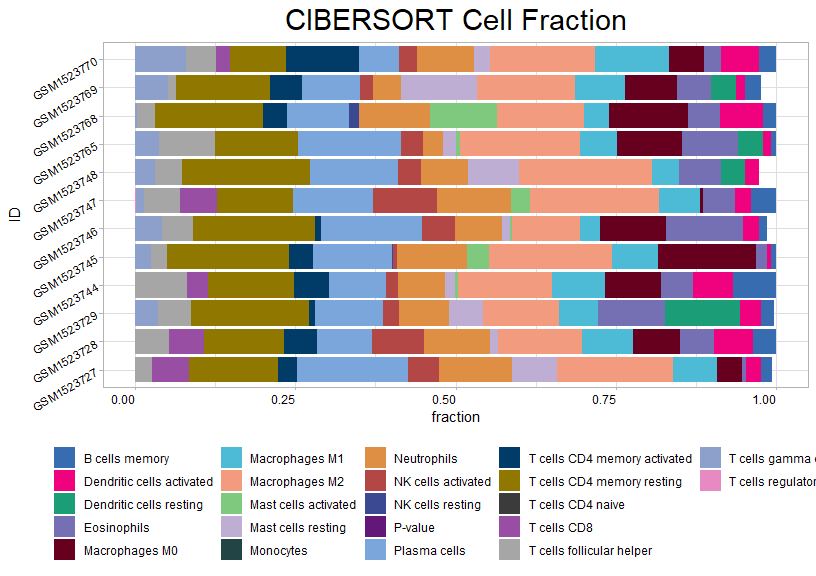
\includegraphics{Feature-selections_files/figure-latex/unnamed-chunk-7-1} \end{center}

\hypertarget{visulization-using-heatmap}{%
\section{Visulization using heatmap}\label{visulization-using-heatmap}}

Relationship between Signatures and molecular typing.
Heatmap visualisation using \texttt{IOBR}'s \texttt{sig\_heatmap}

\begin{Shaded}
\begin{Highlighting}[]
\NormalTok{p2 }\OtherTok{\textless{}{-}} \FunctionTok{sig\_heatmap}\NormalTok{(}\AttributeTok{input         =}\NormalTok{ input, }
                  \AttributeTok{features      =}\NormalTok{ res}\SpecialCharTok{$}\NormalTok{ID[}\DecValTok{1}\SpecialCharTok{:}\DecValTok{20}\NormalTok{],}
                  \AttributeTok{group         =} \StringTok{"Subtype"}\NormalTok{, }
                  \AttributeTok{palette\_group =} \StringTok{"jama"}\NormalTok{, }
                  \AttributeTok{palette       =} \DecValTok{6}\NormalTok{,}
                  \AttributeTok{path          =} \StringTok{"result"}\NormalTok{ )}
\end{Highlighting}
\end{Shaded}

\begin{center}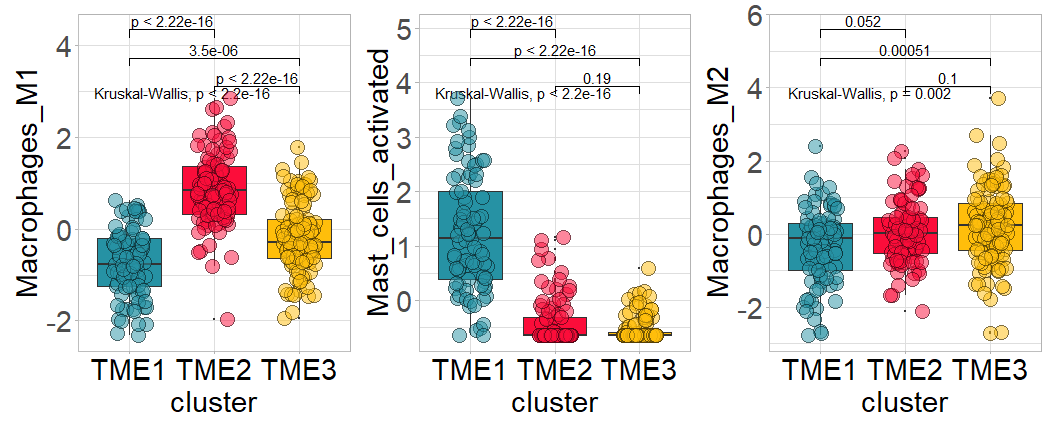
\includegraphics{Feature-selections_files/figure-latex/unnamed-chunk-8-1} \end{center}

\hypertarget{focus-on-target-signatures}{%
\section{Focus on target signatures}\label{focus-on-target-signatures}}

\begin{Shaded}
\begin{Highlighting}[]
\NormalTok{p1 }\OtherTok{\textless{}{-}} \FunctionTok{sig\_box}\NormalTok{(}\AttributeTok{data           =}\NormalTok{ input, }
              \AttributeTok{signature      =} \StringTok{"Glycogen\_Biosynthesis"}\NormalTok{,}
              \AttributeTok{variable       =} \StringTok{"Subtype"}\NormalTok{,}
              \AttributeTok{jitter         =} \ConstantTok{FALSE}\NormalTok{,}
              \AttributeTok{cols           =}  \ConstantTok{NULL}\NormalTok{,}
              \AttributeTok{palette        =} \StringTok{"jama"}\NormalTok{,}
              \AttributeTok{show\_pvalue    =} \ConstantTok{TRUE}\NormalTok{,}
              \AttributeTok{size\_of\_pvalue =} \DecValTok{5}\NormalTok{,}
              \AttributeTok{hjust          =} \DecValTok{1}\NormalTok{, }
              \AttributeTok{angle\_x\_text   =} \DecValTok{60}\NormalTok{, }
              \AttributeTok{size\_of\_font   =} \DecValTok{8}\NormalTok{)}
\end{Highlighting}
\end{Shaded}

\begin{verbatim}
## # A tibble: 6 x 8
##   .y.       group1    group2           p    p.adj p.format p.signif method  
##   <chr>     <chr>     <chr>        <dbl>    <dbl> <chr>    <chr>    <chr>   
## 1 signature EMT       MSI       5.39e-15 3.20e-14 5.4e-15  ****     Wilcoxon
## 2 signature EMT       MSS/TP53- 5.53e-13 2.8 e-12 5.5e-13  ****     Wilcoxon
## 3 signature EMT       MSS/TP53+ 1.90e-12 7.6 e-12 1.9e-12  ****     Wilcoxon
## 4 signature MSI       MSS/TP53- 1.14e- 3 3.4 e- 3 0.0011   **       Wilcoxon
## 5 signature MSI       MSS/TP53+ 7.05e- 3 1.4 e- 2 0.0071   **       Wilcoxon
## 6 signature MSS/TP53- MSS/TP53+ 7.16e- 1 7.2 e- 1 0.7161   ns       Wilcoxon
\end{verbatim}

\begin{Shaded}
\begin{Highlighting}[]
\NormalTok{p2 }\OtherTok{\textless{}{-}} \FunctionTok{sig\_box}\NormalTok{(}\AttributeTok{data           =}\NormalTok{ input, }
              \AttributeTok{signature      =} \StringTok{"Pan\_F\_TBRs"}\NormalTok{,}
              \AttributeTok{variable       =} \StringTok{"Subtype"}\NormalTok{,}
              \AttributeTok{jitter         =} \ConstantTok{FALSE}\NormalTok{,}
              \AttributeTok{cols           =} \ConstantTok{NULL}\NormalTok{,}
              \AttributeTok{palette        =} \StringTok{"jama"}\NormalTok{,}
              \AttributeTok{show\_pvalue    =} \ConstantTok{TRUE}\NormalTok{,}
              \AttributeTok{angle\_x\_text   =} \DecValTok{60}\NormalTok{, }
              \AttributeTok{hjust          =} \DecValTok{1}\NormalTok{, }
              \AttributeTok{size\_of\_pvalue =} \DecValTok{5}\NormalTok{, }
              \AttributeTok{size\_of\_font   =} \DecValTok{8}\NormalTok{)}
\end{Highlighting}
\end{Shaded}

\begin{verbatim}
## # A tibble: 6 x 8
##   .y.       group1    group2           p    p.adj p.format p.signif method  
##   <chr>     <chr>     <chr>        <dbl>    <dbl> <chr>    <chr>    <chr>   
## 1 signature EMT       MSI       7.98e-17 3.20e-16 <2e-16   ****     Wilcoxon
## 2 signature EMT       MSS/TP53- 1.70e-17 1   e-16 <2e-16   ****     Wilcoxon
## 3 signature EMT       MSS/TP53+ 2.57e-17 1.3 e-16 <2e-16   ****     Wilcoxon
## 4 signature MSI       MSS/TP53- 1.32e- 2 4   e- 2 0.013    *        Wilcoxon
## 5 signature MSI       MSS/TP53+ 6.99e- 2 1.4 e- 1 0.070    ns       Wilcoxon
## 6 signature MSS/TP53- MSS/TP53+ 4.02e- 1 4   e- 1 0.402    ns       Wilcoxon
\end{verbatim}

\begin{Shaded}
\begin{Highlighting}[]
\NormalTok{p3 }\OtherTok{\textless{}{-}} \FunctionTok{sig\_box}\NormalTok{(}\AttributeTok{data           =}\NormalTok{ input, }
              \AttributeTok{signature      =} \StringTok{"Immune\_Checkpoint"}\NormalTok{,}
              \AttributeTok{variable       =} \StringTok{"Subtype"}\NormalTok{,}
              \AttributeTok{jitter         =} \ConstantTok{FALSE}\NormalTok{,}
              \AttributeTok{cols           =} \ConstantTok{NULL}\NormalTok{,}
              \AttributeTok{palette        =} \StringTok{"jama"}\NormalTok{,}
              \AttributeTok{show\_pvalue    =} \ConstantTok{TRUE}\NormalTok{,}
              \AttributeTok{angle\_x\_text   =} \DecValTok{60}\NormalTok{, }
              \AttributeTok{hjust          =} \DecValTok{1}\NormalTok{, }
              \AttributeTok{size\_of\_pvalue =} \DecValTok{5}\NormalTok{, }
              \AttributeTok{size\_of\_font   =} \DecValTok{8}\NormalTok{)}
\end{Highlighting}
\end{Shaded}

\begin{verbatim}
## # A tibble: 6 x 8
##   .y.       group1    group2           p        p.adj p.format p.signif method  
##   <chr>     <chr>     <chr>        <dbl>        <dbl> <chr>    <chr>    <chr>   
## 1 signature EMT       MSI       2.20e- 2 0.044        0.0220   *        Wilcoxon
## 2 signature EMT       MSS/TP53- 2.11e- 3 0.0085       0.0021   **       Wilcoxon
## 3 signature EMT       MSS/TP53+ 4.03e- 1 0.4          0.4026   ns       Wilcoxon
## 4 signature MSI       MSS/TP53- 9.13e-10 0.0000000055 9.1e-10  ****     Wilcoxon
## 5 signature MSI       MSS/TP53+ 5.03e- 4 0.0025       0.0005   ***      Wilcoxon
## 6 signature MSS/TP53- MSS/TP53+ 4.82e- 3 0.014        0.0048   **       Wilcoxon
\end{verbatim}

\begin{Shaded}
\begin{Highlighting}[]
\NormalTok{p1}\SpecialCharTok{|}\NormalTok{p2}\SpecialCharTok{|}\NormalTok{p3}
\end{Highlighting}
\end{Shaded}

\begin{center}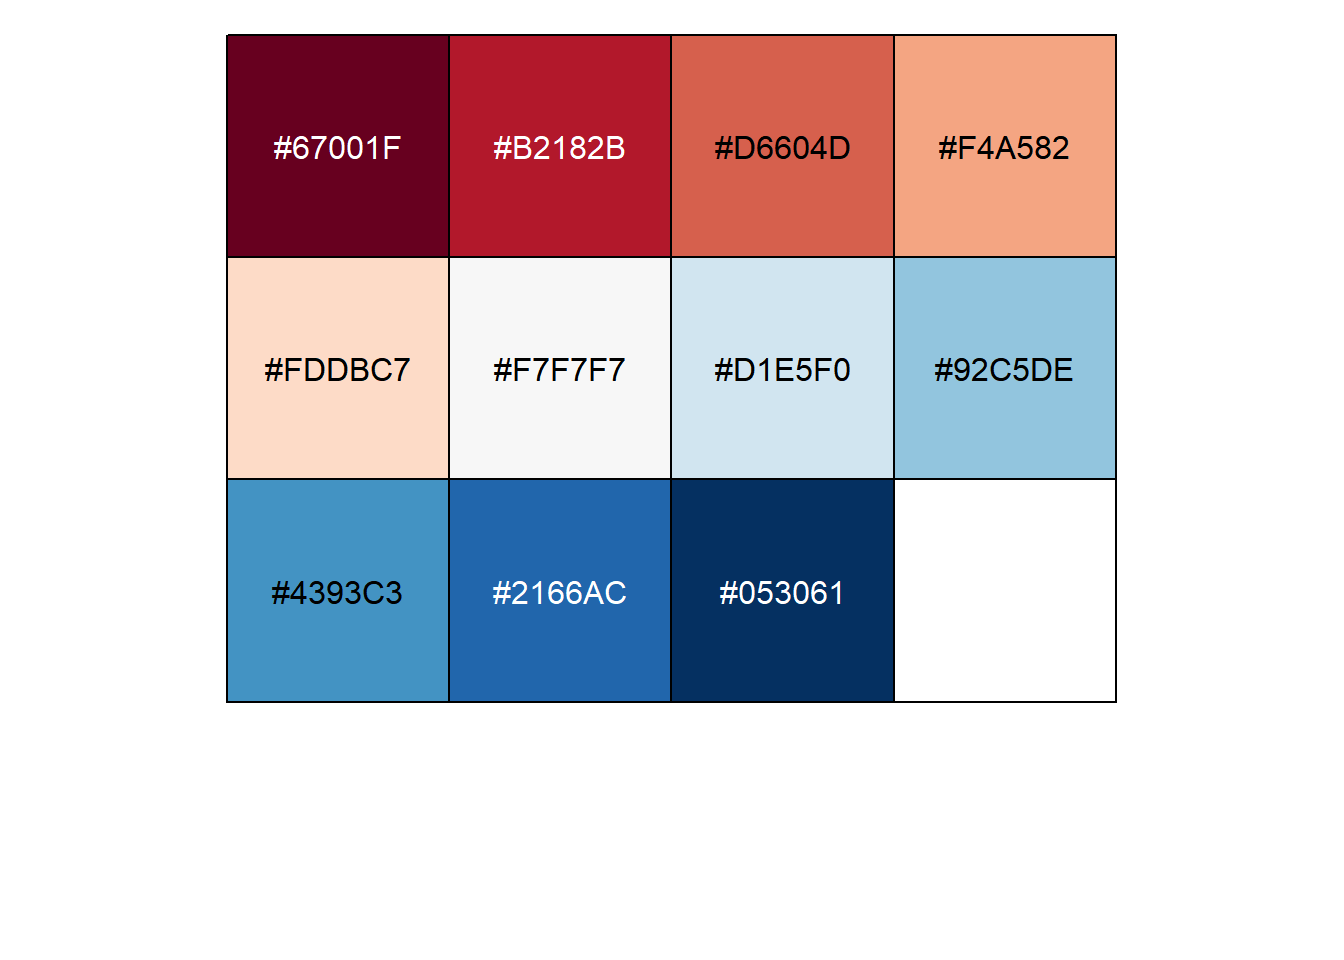
\includegraphics{Feature-selections_files/figure-latex/unnamed-chunk-10-1} \end{center}

\hypertarget{survival-analysis-and-visulization}{%
\section{Survival analysis and visulization}\label{survival-analysis-and-visulization}}

\hypertarget{kaplan-meier-plot}{%
\subsection{Kaplan-Meier plot}\label{kaplan-meier-plot}}

Displaying the outcomes of survival analyses using Kaplan-Meier plot. Multiple stratifications of the signature were used to judge the efficacy of this metric in predicting patient survival.

\begin{Shaded}
\begin{Highlighting}[]
\NormalTok{res }\OtherTok{\textless{}{-}}       \FunctionTok{sig\_surv\_plot}\NormalTok{(}\AttributeTok{input\_pdata       =}\NormalTok{ input, }
                           \AttributeTok{signature         =} \StringTok{"Glycogen\_Biosynthesis"}\NormalTok{,}
                           \AttributeTok{cols              =} \ConstantTok{NULL}\NormalTok{, }
                           \AttributeTok{palette           =} \StringTok{"jama"}\NormalTok{,}
                           \AttributeTok{project           =} \StringTok{"ACRG"}\NormalTok{,}
                           \AttributeTok{time              =} \StringTok{"OS\_time"}\NormalTok{,}
                           \AttributeTok{status            =} \StringTok{"OS\_status"}\NormalTok{,}
                           \AttributeTok{time\_type         =} \StringTok{"month"}\NormalTok{,}
                           \AttributeTok{save\_path         =} \StringTok{"result"}\NormalTok{)}
\end{Highlighting}
\end{Shaded}

\begin{verbatim}
##           ID   time status Glycogen_Biosynthesis group3 group2 bestcutoff
## 1 GSM1523727  88.73      0            -0.3612213 Middle    Low        Low
## 2 GSM1523728  88.23      0            -0.6926726    Low    Low        Low
## 3 GSM1523729  88.23      0            -0.9388531    Low    Low        Low
## 4 GSM1523744 105.70      0            -1.1825136    Low    Low        Low
## 5 GSM1523745 105.53      0            -0.3034304 Middle    Low        Low
## 6 GSM1523746  25.50      1             0.7517934   High   High       High
\end{verbatim}

\begin{verbatim}
## [1] ">>>>>>>>>"
\end{verbatim}

\begin{Shaded}
\begin{Highlighting}[]
\NormalTok{res}\SpecialCharTok{$}\NormalTok{plots}
\end{Highlighting}
\end{Shaded}

\includegraphics{Feature-selections_files/figure-latex/unnamed-chunk-11-1.pdf}

\hypertarget{time-dependent-roc-curve}{%
\subsection{Time-Dependent ROC curve}\label{time-dependent-roc-curve}}

\begin{Shaded}
\begin{Highlighting}[]
\NormalTok{p1}\OtherTok{\textless{}{-}} \FunctionTok{roc\_time}\NormalTok{(}\AttributeTok{input      =}\NormalTok{ input,  }
             \AttributeTok{vars       =} \StringTok{"Glycogen\_Biosynthesis"}\NormalTok{, }
             \AttributeTok{time       =} \StringTok{"OS\_time"}\NormalTok{,}
             \AttributeTok{status     =} \StringTok{"OS\_status"}\NormalTok{, }
             \AttributeTok{time\_point =} \FunctionTok{c}\NormalTok{(}\DecValTok{12}\NormalTok{, }\DecValTok{24}\NormalTok{, }\DecValTok{36}\NormalTok{), }
             \AttributeTok{time\_type  =} \StringTok{"month"}\NormalTok{,}
             \AttributeTok{palette    =} \StringTok{"jama"}\NormalTok{,}
             \AttributeTok{cols       =} \StringTok{"normal"}\NormalTok{,}
             \AttributeTok{seed       =} \DecValTok{1234}\NormalTok{, }
             \AttributeTok{show\_col   =} \ConstantTok{FALSE}\NormalTok{, }
             \AttributeTok{path       =} \StringTok{"result"}\NormalTok{, }
             \AttributeTok{main       =} \StringTok{"OS"}\NormalTok{,}
             \AttributeTok{index      =} \DecValTok{1}\NormalTok{,}
             \AttributeTok{fig.type   =} \StringTok{"pdf"}\NormalTok{,}
             \AttributeTok{width      =} \DecValTok{5}\NormalTok{,}
             \AttributeTok{height     =} \FloatTok{5.2}\NormalTok{)}
\end{Highlighting}
\end{Shaded}

\begin{verbatim}
## [1] ">>>-- Range of Time: "
## [1]   1.0 105.7
\end{verbatim}

\begin{Shaded}
\begin{Highlighting}[]
\NormalTok{p2}\OtherTok{\textless{}{-}} \FunctionTok{roc\_time}\NormalTok{(}\AttributeTok{input      =}\NormalTok{ input,  }
             \AttributeTok{vars       =} \StringTok{"Glycogen\_Biosynthesis"}\NormalTok{, }
             \AttributeTok{time       =} \StringTok{"RFS\_time"}\NormalTok{,}
             \AttributeTok{status     =} \StringTok{"RFS\_status"}\NormalTok{, }
             \AttributeTok{time\_point =} \FunctionTok{c}\NormalTok{(}\DecValTok{12}\NormalTok{, }\DecValTok{24}\NormalTok{, }\DecValTok{36}\NormalTok{), }
             \AttributeTok{time\_type  =} \StringTok{"month"}\NormalTok{,}
             \AttributeTok{palette    =} \StringTok{"jama"}\NormalTok{,}
             \AttributeTok{cols       =} \StringTok{"normal"}\NormalTok{,}
             \AttributeTok{seed       =} \DecValTok{1234}\NormalTok{, }
             \AttributeTok{show\_col   =} \ConstantTok{FALSE}\NormalTok{, }
             \AttributeTok{path       =} \StringTok{"result"}\NormalTok{, }
             \AttributeTok{main       =} \StringTok{"OS"}\NormalTok{,}
             \AttributeTok{index      =} \DecValTok{1}\NormalTok{,}
             \AttributeTok{fig.type   =} \StringTok{"pdf"}\NormalTok{,}
             \AttributeTok{width      =} \DecValTok{5}\NormalTok{,}
             \AttributeTok{height     =} \FloatTok{5.2}\NormalTok{)}
\end{Highlighting}
\end{Shaded}

\begin{verbatim}
## [1] ">>>-- Range of Time: "
## [1]   0.10 100.87
\end{verbatim}

\begin{Shaded}
\begin{Highlighting}[]
\NormalTok{p1}\SpecialCharTok{|}\NormalTok{p2}
\end{Highlighting}
\end{Shaded}

\includegraphics{Feature-selections_files/figure-latex/unnamed-chunk-12-1.pdf}

\hypertarget{batch-correlation-analysis}{%
\section{Batch correlation analysis}\label{batch-correlation-analysis}}

\hypertarget{finding-continuity-variables-associated-with-signatures}{%
\subsection{Finding continuity variables associated with signatures}\label{finding-continuity-variables-associated-with-signatures}}

Identifying genes or signatures related to the target signatures

\hypertarget{correlation-between-two-variables}{%
\subsubsection{Correlation between two variables}\label{correlation-between-two-variables}}

\begin{Shaded}
\begin{Highlighting}[]
\NormalTok{res }\OtherTok{\textless{}{-}} \FunctionTok{batch\_cor}\NormalTok{(}\AttributeTok{data =}\NormalTok{ input, }\AttributeTok{target =} \StringTok{"Glycogen\_Biosynthesis"}\NormalTok{, }\AttributeTok{feature =} \FunctionTok{colnames}\NormalTok{(input)[}\DecValTok{69}\SpecialCharTok{:}\FunctionTok{ncol}\NormalTok{(input)])}
\end{Highlighting}
\end{Shaded}

\begin{verbatim}
##                               sig_names      p.value   statistic
## CD_8_T_effector.rho     CD_8_T_effector 4.852189e-01 -0.04044756
## DDR.rho                             DDR 1.678463e-24 -0.54394827
## APM.rho                             APM 1.681208e-04 -0.21557706
## Immune_Checkpoint.rho Immune_Checkpoint 6.470746e-01 -0.02653896
## CellCycle_Reg.rho         CellCycle_Reg 4.465875e-01 -0.04410582
## Pan_F_TBRs.rho               Pan_F_TBRs 5.989600e-31  0.60185558
\end{verbatim}

\begin{Shaded}
\begin{Highlighting}[]
\FunctionTok{head}\NormalTok{(res)}
\end{Highlighting}
\end{Shaded}

\begin{verbatim}
## # A tibble: 6 x 6
##   sig_names                         p.value statistic    p.adj log10pvalue stars
##   <chr>                               <dbl>     <dbl>    <dbl>       <dbl> <fct>
## 1 TMEscoreB_CIR                    8.89e-42     0.678 2.27e-39        41.1 **** 
## 2 Glycine__Serine_and_Threonine_M~ 7.49e-40    -0.666 9.54e-38        39.1 **** 
## 3 Ether_Lipid_Metabolism           3.84e-39     0.662 3.27e-37        38.4 **** 
## 4 MDSC_Peng_et_al                  1.13e-38     0.659 7.21e-37        37.9 **** 
## 5 Glycerophospholipid_Metabolism   8.72e-38    -0.653 4.44e-36        37.1 **** 
## 6 TIP_Release_of_cancer_cell_anti~ 2.32e-37    -0.650 9.86e-36        36.6 ****
\end{verbatim}

\begin{Shaded}
\begin{Highlighting}[]
\NormalTok{p1}\OtherTok{\textless{}{-}} \FunctionTok{get\_cor}\NormalTok{(}\AttributeTok{eset =}\NormalTok{ sig\_tme, }\AttributeTok{pdata =}\NormalTok{ pdata\_acrg, }\AttributeTok{is.matrix =} \ConstantTok{TRUE}\NormalTok{, }\AttributeTok{var1 =} \StringTok{"Glycogen\_Biosynthesis"}\NormalTok{, }
             \AttributeTok{var2 =} \StringTok{"TMEscore\_CIR"}\NormalTok{, }\AttributeTok{subtype =} \StringTok{"Subtype"}\NormalTok{, }\AttributeTok{palette =} \StringTok{"aaas"}\NormalTok{, }\AttributeTok{path =} \StringTok{"result"}\NormalTok{)}
\end{Highlighting}
\end{Shaded}

\begin{verbatim}
## 
##  Spearman's rank correlation rho
## 
## data:  data[, var1] and data[, var2]
## S = 7282858, p-value < 2.2e-16
## alternative hypothesis: true rho is not equal to 0
## sample estimates:
##        rho 
## -0.6184309 
## 
## [1] ">>>--- The exact p value is: 4.78971420439895e-33"
##       EMT       MSI MSS/TP53- MSS/TP53+ 
##        46        68       107        79
\end{verbatim}

\begin{Shaded}
\begin{Highlighting}[]
\NormalTok{p2}\OtherTok{\textless{}{-}} \FunctionTok{get\_cor}\NormalTok{(}\AttributeTok{eset =}\NormalTok{ sig\_tme, }\AttributeTok{pdata =}\NormalTok{ pdata\_acrg, }\AttributeTok{is.matrix =} \ConstantTok{TRUE}\NormalTok{, }\AttributeTok{var1 =} \StringTok{"Glycogen\_Biosynthesis"}\NormalTok{, }
             \AttributeTok{var2 =} \StringTok{"TGFb.myCAF"}\NormalTok{, }\AttributeTok{subtype =} \StringTok{"Subtype"}\NormalTok{, }\AttributeTok{palette =} \StringTok{"aaas"}\NormalTok{, }\AttributeTok{path =} \StringTok{"result"}\NormalTok{)}
\end{Highlighting}
\end{Shaded}

\begin{verbatim}
## 
##  Spearman's rank correlation rho
## 
## data:  data[, var1] and data[, var2]
## S = 2471758, p-value < 2.2e-16
## alternative hypothesis: true rho is not equal to 0
## sample estimates:
##       rho 
## 0.4507143 
## 
## [1] ">>>--- The exact p value is: 2.04505761057615e-16"
##       EMT       MSI MSS/TP53- MSS/TP53+ 
##        46        68       107        79
\end{verbatim}

\begin{Shaded}
\begin{Highlighting}[]
\NormalTok{p1}\SpecialCharTok{|}\NormalTok{p2}
\end{Highlighting}
\end{Shaded}

\includegraphics{Feature-selections_files/figure-latex/unnamed-chunk-15-1.pdf}

\hypertarget{demonstrate-correlation-between-multiple-variables}{%
\subsubsection{Demonstrate correlation between multiple variables}\label{demonstrate-correlation-between-multiple-variables}}

Visualisation via correlation matrix

\begin{Shaded}
\begin{Highlighting}[]
\NormalTok{feas1 }\OtherTok{\textless{}{-}} \FunctionTok{c}\NormalTok{(}\StringTok{"Glycogen\_Biosynthesis"}\NormalTok{, }\StringTok{"Ferroptosis"}\NormalTok{)}
\NormalTok{feas2 }\OtherTok{\textless{}{-}} \FunctionTok{c}\NormalTok{(}\StringTok{"Glutathione\_Metabolism"}\NormalTok{, }\StringTok{"TMEscore\_CIR"}\NormalTok{, }\StringTok{"Purine\_Metabolism"}\NormalTok{, }\StringTok{"ICB\_resistance\_Peng\_et\_al"}\NormalTok{, }\StringTok{"Interleukins\_Li\_et\_al"}\NormalTok{, }\StringTok{"TLS\_Nature"}\NormalTok{)}
\NormalTok{p }\OtherTok{\textless{}{-}} \FunctionTok{get\_cor\_matrix}\NormalTok{(}\AttributeTok{data           =}\NormalTok{ input, }
                    \AttributeTok{feas1          =}\NormalTok{ feas2, }
                    \AttributeTok{feas2          =}\NormalTok{ feas1,}
                    \AttributeTok{method         =} \StringTok{"pearson"}\NormalTok{,}
                    \AttributeTok{font.size.star =} \DecValTok{8}\NormalTok{, }
                    \AttributeTok{font.size      =} \DecValTok{15}\NormalTok{, }
                    \AttributeTok{fill\_by\_cor    =} \ConstantTok{FALSE}\NormalTok{, }
                    \AttributeTok{round.num      =} \DecValTok{1}\NormalTok{, }
                    \AttributeTok{path           =} \StringTok{"result"}\NormalTok{)}
\end{Highlighting}
\end{Shaded}

\includegraphics{Feature-selections_files/figure-latex/unnamed-chunk-16-1.pdf}

Demonstrate the correlation between signatures and genes

\begin{Shaded}
\begin{Highlighting}[]
\NormalTok{input2 }\OtherTok{\textless{}{-}} \FunctionTok{combine\_pd\_eset}\NormalTok{(}\AttributeTok{eset =}\NormalTok{ eset, }\AttributeTok{pdata =}\NormalTok{  input[, }\FunctionTok{c}\NormalTok{(}\StringTok{"ID"}\NormalTok{, }\StringTok{"Glycogen\_Biosynthesis"}\NormalTok{, }\StringTok{"TLS\_Nature"}\NormalTok{, }\StringTok{"Ferroptosis"}\NormalTok{)])}
\NormalTok{feas1 }\OtherTok{\textless{}{-}} \FunctionTok{c}\NormalTok{(}\StringTok{"Glycogen\_Biosynthesis"}\NormalTok{,}\StringTok{"TLS\_Nature"}\NormalTok{, }\StringTok{"Ferroptosis"}\NormalTok{)}
\NormalTok{feas2 }\OtherTok{\textless{}{-}}\NormalTok{ signature\_collection}\SpecialCharTok{$}\NormalTok{CD\_8\_T\_effector}
\NormalTok{feas2}
\end{Highlighting}
\end{Shaded}

\begin{verbatim}
## [1] "CD8A"   "GZMA"   "GZMB"   "IFNG"   "CXCL9"  "CXCL10" "PRF1"   "TBX21"
\end{verbatim}

\begin{Shaded}
\begin{Highlighting}[]
\NormalTok{p }\OtherTok{\textless{}{-}} \FunctionTok{get\_cor\_matrix}\NormalTok{(}\AttributeTok{data           =}\NormalTok{ input2, }
                    \AttributeTok{feas1          =}\NormalTok{ feas2, }
                    \AttributeTok{feas2          =}\NormalTok{ feas1,}
                    \AttributeTok{method         =} \StringTok{"pearson"}\NormalTok{,}
                    \AttributeTok{scale          =}\NormalTok{ T, }
                    \AttributeTok{font.size.star =} \DecValTok{8}\NormalTok{, }
                    \AttributeTok{font.size      =} \DecValTok{15}\NormalTok{, }
                    \AttributeTok{fill\_by\_cor    =} \ConstantTok{FALSE}\NormalTok{, }
                    \AttributeTok{round.num      =} \DecValTok{1}\NormalTok{,}
                    \AttributeTok{path           =} \StringTok{"result"}\NormalTok{)}
\end{Highlighting}
\end{Shaded}

\includegraphics{Feature-selections_files/figure-latex/unnamed-chunk-17-1.pdf}

Users can customize the image using parameters.

\begin{Shaded}
\begin{Highlighting}[]
\NormalTok{p }\OtherTok{\textless{}{-}} \FunctionTok{get\_cor\_matrix}\NormalTok{(}\AttributeTok{data           =}\NormalTok{ input2, }
                    \AttributeTok{feas1          =}\NormalTok{ feas2, }
                    \AttributeTok{feas2          =}\NormalTok{ feas1,}
                    \AttributeTok{method         =} \StringTok{"pearson"}\NormalTok{,}
                    \AttributeTok{scale          =}\NormalTok{ T, }
                    \AttributeTok{font.size.star =} \DecValTok{8}\NormalTok{, }
                    \AttributeTok{font.size      =} \DecValTok{15}\NormalTok{, }
                    \AttributeTok{fill\_by\_cor    =} \ConstantTok{TRUE}\NormalTok{, }
                    \AttributeTok{round.num      =} \DecValTok{2}\NormalTok{,}
                    \AttributeTok{path           =} \StringTok{"result"}\NormalTok{)}
\end{Highlighting}
\end{Shaded}

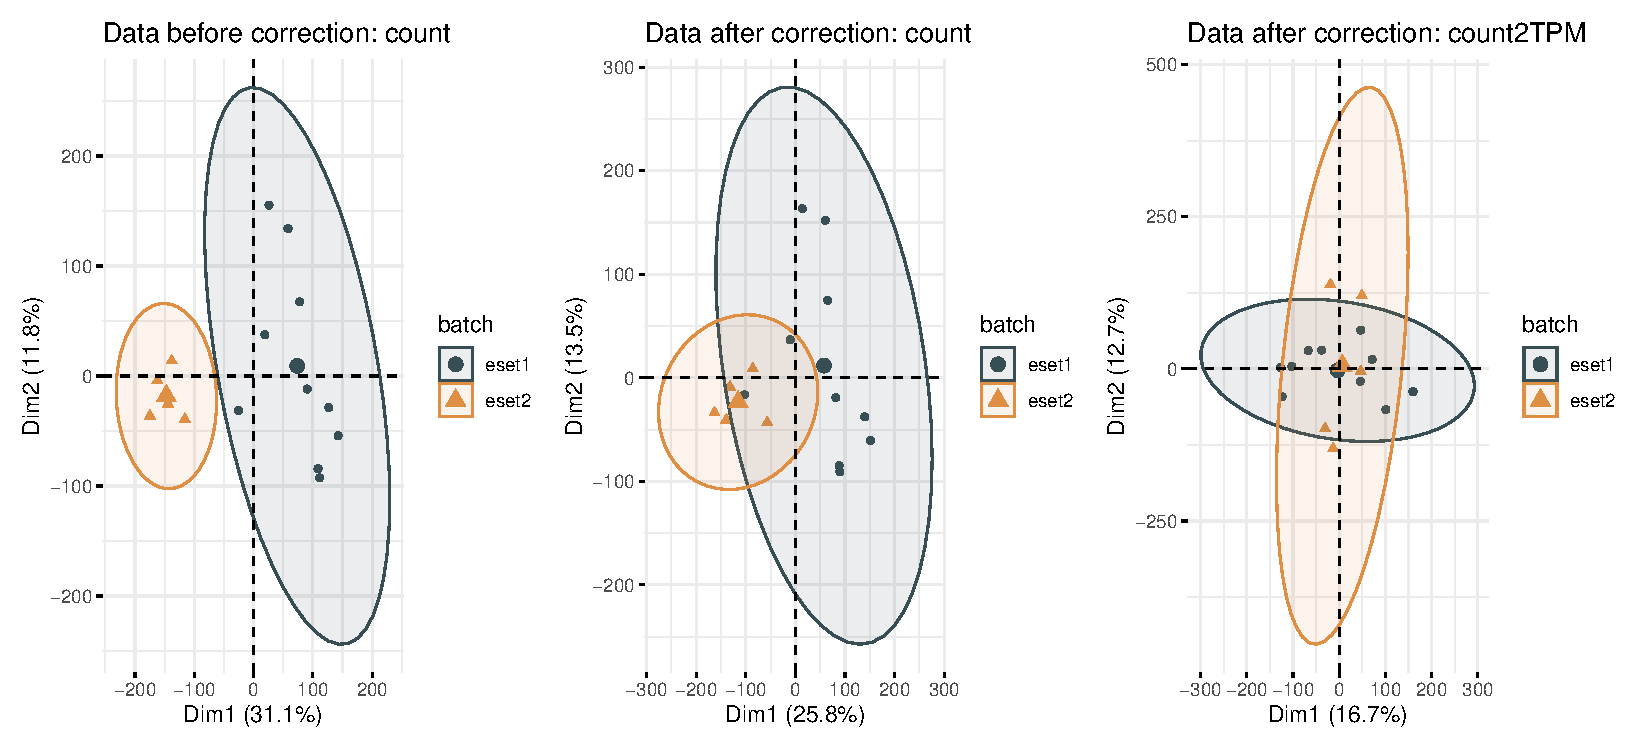
\includegraphics{Feature-selections_files/figure-latex/unnamed-chunk-18-1.pdf}

\hypertarget{identifying-category-variables-linked-to-signatures}{%
\subsection{Identifying Category Variables Linked to Signatures}\label{identifying-category-variables-linked-to-signatures}}

\hypertarget{for-binary-variable}{%
\subsubsection{For binary variable}\label{for-binary-variable}}

\begin{Shaded}
\begin{Highlighting}[]
\NormalTok{res }\OtherTok{\textless{}{-}} \FunctionTok{batch\_wilcoxon}\NormalTok{(}\AttributeTok{data =}\NormalTok{ input, }\AttributeTok{target =} \StringTok{"TMEscore\_binary"}\NormalTok{, }\AttributeTok{feature =} \FunctionTok{colnames}\NormalTok{(input)[}\DecValTok{69}\SpecialCharTok{:}\FunctionTok{ncol}\NormalTok{(input)])}
\end{Highlighting}
\end{Shaded}

\begin{verbatim}
## 
## High  Low 
##   71  228
\end{verbatim}

\begin{Shaded}
\begin{Highlighting}[]
\FunctionTok{head}\NormalTok{(res)}
\end{Highlighting}
\end{Shaded}

\begin{verbatim}
## # A tibble: 6 x 8
##   sig_names         p.value   High    Low statistic    p.adj log10pvalue stars
##   <chr>               <dbl>  <dbl>  <dbl>     <dbl>    <dbl>       <dbl> <fct>
## 1 TMEscore_CIR     4.44e-37  1.17  -0.365      1.54 1.14e-34        36.4 **** 
## 2 TMEscore_plus    3.97e-34  1.23  -0.380      1.61 5.08e-32        33.4 **** 
## 3 TMEscoreA_plus   1.68e-25  1.18  -0.359      1.54 1.44e-23        24.8 **** 
## 4 TMEscoreB_CIR    5.59e-24 -0.881  0.279     -1.16 3.36e-22        23.3 **** 
## 5 ADP_Ribosylation 6.56e-24  1.06  -0.329      1.39 3.36e-22        23.2 **** 
## 6 TMEscoreA_CIR    1.02e-22  1.11  -0.337      1.45 3.80e-21        22.0 ****
\end{verbatim}

\begin{Shaded}
\begin{Highlighting}[]
\NormalTok{p1 }\OtherTok{\textless{}{-}} \FunctionTok{sig\_box}\NormalTok{(}\AttributeTok{data           =}\NormalTok{ input, }
              \AttributeTok{signature      =}\NormalTok{ res}\SpecialCharTok{$}\NormalTok{sig\_names[}\DecValTok{1}\NormalTok{],}
              \AttributeTok{variable       =} \StringTok{"TMEscore\_binary"}\NormalTok{,}
              \AttributeTok{jitter         =} \ConstantTok{FALSE}\NormalTok{,}
              \AttributeTok{cols           =}  \ConstantTok{NULL}\NormalTok{,}
              \AttributeTok{palette        =} \StringTok{"jco"}\NormalTok{,}
              \AttributeTok{show\_pvalue    =} \ConstantTok{TRUE}\NormalTok{,}
              \AttributeTok{size\_of\_pvalue =} \DecValTok{5}\NormalTok{,}
              \AttributeTok{hjust          =} \DecValTok{1}\NormalTok{, }
              \AttributeTok{angle\_x\_text   =} \DecValTok{60}\NormalTok{, }
              \AttributeTok{size\_of\_font   =} \DecValTok{8}\NormalTok{)}
\end{Highlighting}
\end{Shaded}

\begin{verbatim}
## # A tibble: 1 x 8
##   .y.       group1 group2        p    p.adj p.format p.signif method  
##   <chr>     <chr>  <chr>     <dbl>    <dbl> <chr>    <chr>    <chr>   
## 1 signature High   Low    4.44e-37 4.40e-37 <2e-16   ****     Wilcoxon
\end{verbatim}

\begin{Shaded}
\begin{Highlighting}[]
\NormalTok{p2 }\OtherTok{\textless{}{-}} \FunctionTok{sig\_box}\NormalTok{(}\AttributeTok{data           =}\NormalTok{ input, }
              \AttributeTok{signature      =}\NormalTok{ res}\SpecialCharTok{$}\NormalTok{sig\_names[}\DecValTok{2}\NormalTok{],}
              \AttributeTok{variable       =} \StringTok{"TMEscore\_binary"}\NormalTok{,}
              \AttributeTok{jitter         =} \ConstantTok{FALSE}\NormalTok{,}
              \AttributeTok{cols           =} \ConstantTok{NULL}\NormalTok{,}
              \AttributeTok{palette        =} \StringTok{"jco"}\NormalTok{,}
              \AttributeTok{show\_pvalue    =} \ConstantTok{TRUE}\NormalTok{,}
              \AttributeTok{angle\_x\_text   =} \DecValTok{60}\NormalTok{, }
              \AttributeTok{hjust          =} \DecValTok{1}\NormalTok{, }
              \AttributeTok{size\_of\_pvalue =} \DecValTok{5}\NormalTok{, }
              \AttributeTok{size\_of\_font   =} \DecValTok{8}\NormalTok{)}
\end{Highlighting}
\end{Shaded}

\begin{verbatim}
## # A tibble: 1 x 8
##   .y.       group1 group2        p p.adj p.format p.signif method  
##   <chr>     <chr>  <chr>     <dbl> <dbl> <chr>    <chr>    <chr>   
## 1 signature High   Low    3.97e-34 4e-34 <2e-16   ****     Wilcoxon
\end{verbatim}

\begin{Shaded}
\begin{Highlighting}[]
\NormalTok{p3 }\OtherTok{\textless{}{-}} \FunctionTok{sig\_box}\NormalTok{(}\AttributeTok{data           =}\NormalTok{ input, }
              \AttributeTok{signature      =}\NormalTok{ res}\SpecialCharTok{$}\NormalTok{sig\_names[}\DecValTok{3}\NormalTok{],}
              \AttributeTok{variable       =} \StringTok{"TMEscore\_binary"}\NormalTok{,}
              \AttributeTok{jitter         =} \ConstantTok{FALSE}\NormalTok{,}
              \AttributeTok{cols           =} \ConstantTok{NULL}\NormalTok{,}
              \AttributeTok{palette        =} \StringTok{"jco"}\NormalTok{,}
              \AttributeTok{show\_pvalue    =} \ConstantTok{TRUE}\NormalTok{,}
              \AttributeTok{angle\_x\_text   =} \DecValTok{60}\NormalTok{, }
              \AttributeTok{hjust          =} \DecValTok{1}\NormalTok{, }
              \AttributeTok{size\_of\_pvalue =} \DecValTok{5}\NormalTok{, }
              \AttributeTok{size\_of\_font   =} \DecValTok{8}\NormalTok{)}
\end{Highlighting}
\end{Shaded}

\begin{verbatim}
## # A tibble: 1 x 8
##   .y.       group1 group2        p    p.adj p.format p.signif method  
##   <chr>     <chr>  <chr>     <dbl>    <dbl> <chr>    <chr>    <chr>   
## 1 signature High   Low    1.68e-25 1.70e-25 <2e-16   ****     Wilcoxon
\end{verbatim}

\begin{Shaded}
\begin{Highlighting}[]
\NormalTok{p1}\SpecialCharTok{|}\NormalTok{p2}\SpecialCharTok{|}\NormalTok{p3}
\end{Highlighting}
\end{Shaded}

\begin{center}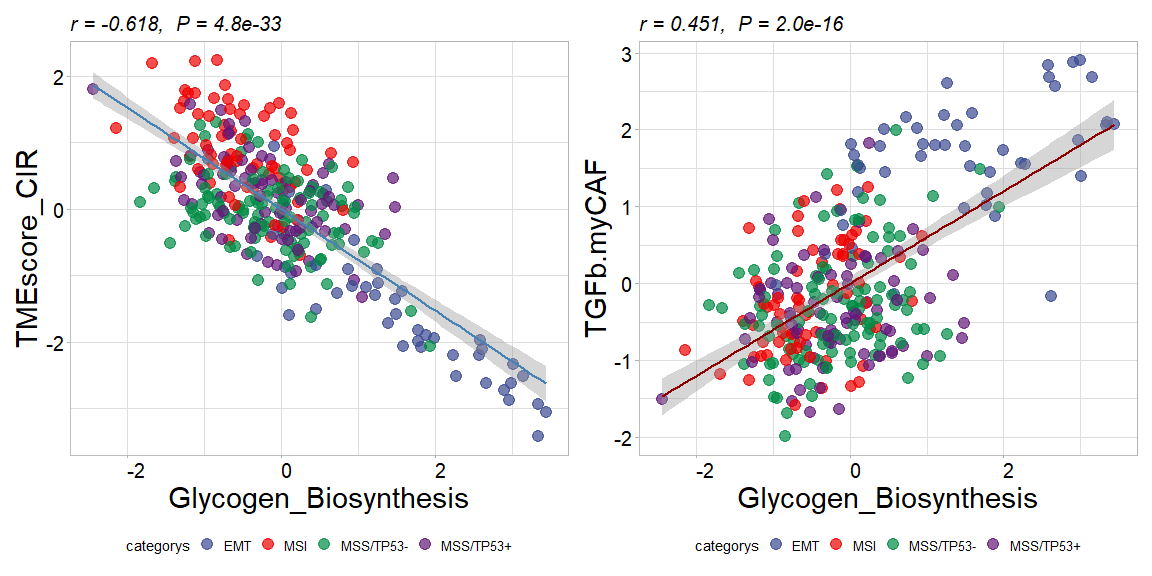
\includegraphics{Feature-selections_files/figure-latex/unnamed-chunk-21-1} \end{center}

\hypertarget{for-multicategorical-variables-2-subgroups}{%
\subsection{For multicategorical variables (\textgreater2 subgroups)}\label{for-multicategorical-variables-2-subgroups}}

\begin{Shaded}
\begin{Highlighting}[]
\NormalTok{res }\OtherTok{\textless{}{-}} \FunctionTok{batch\_kruskal}\NormalTok{(}\AttributeTok{data =}\NormalTok{ input, }\AttributeTok{group =} \StringTok{"Subtype"}\NormalTok{, }\AttributeTok{feature =} \FunctionTok{colnames}\NormalTok{(input)[}\DecValTok{69}\SpecialCharTok{:}\FunctionTok{ncol}\NormalTok{(input)])}
\end{Highlighting}
\end{Shaded}

\begin{verbatim}
## 
##       EMT       MSI MSS/TP53- MSS/TP53+ 
##        46        68       107        79
\end{verbatim}

\begin{Shaded}
\begin{Highlighting}[]
\FunctionTok{head}\NormalTok{(res)}
\end{Highlighting}
\end{Shaded}

\begin{verbatim}
## # A tibble: 6 x 10
##   sig_names        p.value   EMT    MSI `MSS/TP53-` `MSS/TP53+`    mean    p.adj
##   <chr>              <dbl> <dbl>  <dbl>       <dbl>       <dbl>   <dbl>    <dbl>
## 1 TMEscore_CIR    1.35e-28 -1.36  1.00        0.305      0.0577 -0.119  3.46e-26
## 2 Ether_Lipid_Me~ 4.37e-27  1.46 -0.830      -0.253     -0.375   0.165  4.64e-25
## 3 TMEscoreB_CIR   5.88e-27  1.55 -0.829      -0.420     -0.303   0.169  4.64e-25
## 4 Inositol_Phosp~ 7.25e-27  1.53 -0.808      -0.315     -0.408   0.177  4.64e-25
## 5 Selenocompound~ 1.17e-26 -1.48  0.824       0.328      0.326  -0.163  5.99e-25
## 6 Folate_biosynt~ 1.63e-26 -1.12  1.05        0.127     -0.0573 -0.0792 6.15e-25
## # i 2 more variables: log10pvalue <dbl>, stars <fct>
\end{verbatim}

\begin{Shaded}
\begin{Highlighting}[]
\NormalTok{p1 }\OtherTok{\textless{}{-}} \FunctionTok{sig\_box}\NormalTok{(}\AttributeTok{data           =}\NormalTok{ input, }
              \AttributeTok{signature      =}\NormalTok{ res}\SpecialCharTok{$}\NormalTok{sig\_names[}\DecValTok{1}\NormalTok{],}
              \AttributeTok{variable       =} \StringTok{"Subtype"}\NormalTok{,}
              \AttributeTok{jitter         =} \ConstantTok{FALSE}\NormalTok{,}
              \AttributeTok{cols           =}  \ConstantTok{NULL}\NormalTok{,}
              \AttributeTok{palette        =} \StringTok{"jco"}\NormalTok{,}
              \AttributeTok{show\_pvalue    =} \ConstantTok{TRUE}\NormalTok{,}
              \AttributeTok{size\_of\_pvalue =} \DecValTok{5}\NormalTok{,}
              \AttributeTok{hjust          =} \DecValTok{1}\NormalTok{, }
              \AttributeTok{angle\_x\_text   =} \DecValTok{60}\NormalTok{, }
              \AttributeTok{size\_of\_font   =} \DecValTok{8}\NormalTok{)}
\end{Highlighting}
\end{Shaded}

\begin{verbatim}
## # A tibble: 6 x 8
##   .y.       group1    group2           p    p.adj p.format p.signif method  
##   <chr>     <chr>     <chr>        <dbl>    <dbl> <chr>    <chr>    <chr>   
## 1 signature EMT       MSI       3.64e-17 2.20e-16 < 2e-16  ****     Wilcoxon
## 2 signature EMT       MSS/TP53- 1.08e-13 3.20e-13 1.1e-13  ****     Wilcoxon
## 3 signature EMT       MSS/TP53+ 2.64e-14 1.10e-13 2.6e-14  ****     Wilcoxon
## 4 signature MSI       MSS/TP53- 1.27e-15 6.40e-15 1.3e-15  ****     Wilcoxon
## 5 signature MSI       MSS/TP53+ 5.96e- 9 1.20e- 8 6.0e-09  ****     Wilcoxon
## 6 signature MSS/TP53- MSS/TP53+ 7.71e- 3 7.7 e- 3 0.0077   **       Wilcoxon
\end{verbatim}

\begin{Shaded}
\begin{Highlighting}[]
\NormalTok{p2 }\OtherTok{\textless{}{-}} \FunctionTok{sig\_box}\NormalTok{(}\AttributeTok{data           =}\NormalTok{ input, }
              \AttributeTok{signature      =}\NormalTok{ res}\SpecialCharTok{$}\NormalTok{sig\_names[}\DecValTok{2}\NormalTok{],}
              \AttributeTok{variable       =} \StringTok{"Subtype"}\NormalTok{,}
              \AttributeTok{jitter         =} \ConstantTok{FALSE}\NormalTok{,}
              \AttributeTok{cols           =} \ConstantTok{NULL}\NormalTok{,}
              \AttributeTok{palette        =} \StringTok{"jco"}\NormalTok{,}
              \AttributeTok{show\_pvalue    =} \ConstantTok{TRUE}\NormalTok{,}
              \AttributeTok{angle\_x\_text   =} \DecValTok{60}\NormalTok{, }
              \AttributeTok{hjust          =} \DecValTok{1}\NormalTok{, }
              \AttributeTok{size\_of\_pvalue =} \DecValTok{5}\NormalTok{, }
              \AttributeTok{size\_of\_font   =} \DecValTok{8}\NormalTok{)}
\end{Highlighting}
\end{Shaded}

\begin{verbatim}
## # A tibble: 6 x 8
##   .y.       group1    group2           p    p.adj p.format p.signif method  
##   <chr>     <chr>     <chr>        <dbl>    <dbl> <chr>    <chr>    <chr>   
## 1 signature EMT       MSI       3.76e-19 1.9 e-18 < 2e-16  ****     Wilcoxon
## 2 signature EMT       MSS/TP53- 4.26e-20 2.6 e-19 < 2e-16  ****     Wilcoxon
## 3 signature EMT       MSS/TP53+ 5.19e-18 2.10e-17 < 2e-16  ****     Wilcoxon
## 4 signature MSI       MSS/TP53- 5.43e- 5 1.1 e- 4 5.4e-05  ****     Wilcoxon
## 5 signature MSI       MSS/TP53+ 2.12e- 7 6.40e- 7 2.1e-07  ****     Wilcoxon
## 6 signature MSS/TP53- MSS/TP53+ 2.84e- 1 2.8 e- 1 0.28     ns       Wilcoxon
\end{verbatim}

\begin{Shaded}
\begin{Highlighting}[]
\NormalTok{p3 }\OtherTok{\textless{}{-}} \FunctionTok{sig\_box}\NormalTok{(}\AttributeTok{data           =}\NormalTok{ input, }
              \AttributeTok{signature      =}\NormalTok{ res}\SpecialCharTok{$}\NormalTok{sig\_names[}\DecValTok{3}\NormalTok{],}
              \AttributeTok{variable       =} \StringTok{"Subtype"}\NormalTok{,}
              \AttributeTok{jitter         =} \ConstantTok{FALSE}\NormalTok{,}
              \AttributeTok{cols           =} \ConstantTok{NULL}\NormalTok{,}
              \AttributeTok{palette        =} \StringTok{"jco"}\NormalTok{,}
              \AttributeTok{show\_pvalue    =} \ConstantTok{TRUE}\NormalTok{,}
              \AttributeTok{angle\_x\_text   =} \DecValTok{60}\NormalTok{, }
              \AttributeTok{hjust          =} \DecValTok{1}\NormalTok{, }
              \AttributeTok{size\_of\_pvalue =} \DecValTok{5}\NormalTok{, }
              \AttributeTok{size\_of\_font   =} \DecValTok{8}\NormalTok{)}
\end{Highlighting}
\end{Shaded}

\begin{verbatim}
## # A tibble: 6 x 8
##   .y.       group1    group2           p    p.adj p.format p.signif method  
##   <chr>     <chr>     <chr>        <dbl>    <dbl> <chr>    <chr>    <chr>   
## 1 signature EMT       MSI       9.59e-19 4.80e-18 < 2e-16  ****     Wilcoxon
## 2 signature EMT       MSS/TP53- 6.07e-19 3.60e-18 < 2e-16  ****     Wilcoxon
## 3 signature EMT       MSS/TP53+ 2.89e-18 1.20e-17 < 2e-16  ****     Wilcoxon
## 4 signature MSI       MSS/TP53- 1.48e- 7 4.50e- 7 1.5e-07  ****     Wilcoxon
## 5 signature MSI       MSS/TP53+ 1.44e- 5 2.90e- 5 1.4e-05  ****     Wilcoxon
## 6 signature MSS/TP53- MSS/TP53+ 3.17e- 1 3.2 e- 1 0.32     ns       Wilcoxon
\end{verbatim}

\begin{Shaded}
\begin{Highlighting}[]
\NormalTok{p1}\SpecialCharTok{|}\NormalTok{p2}\SpecialCharTok{|}\NormalTok{p3}
\end{Highlighting}
\end{Shaded}

\begin{center}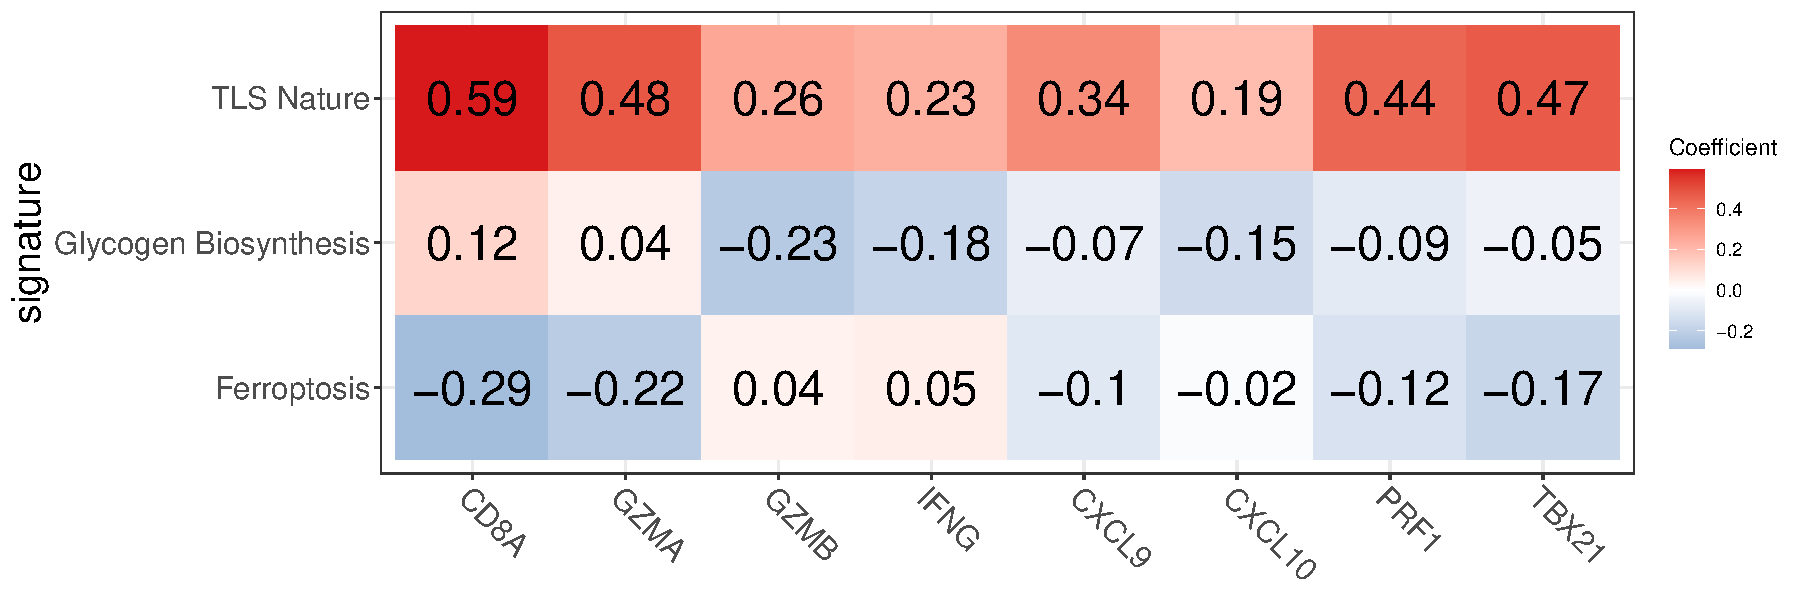
\includegraphics{Feature-selections_files/figure-latex/unnamed-chunk-24-1} \end{center}

\hypertarget{reference}{%
\section{Reference}\label{reference}}

Cristescu, R., Lee, J., Nebozhyn, M. et al.~Molecular analysis of gastric cancer identifies subtypes associated with distinct clinical outcomes. Nat Med 21, 449--456 (2015). \url{https://doi.org/10.1038/nm.3850}

\hypertarget{tme-interaction-analysis}{%
\chapter{\texorpdfstring{\textbf{TME Interaction analysis}}{TME Interaction analysis}}\label{tme-interaction-analysis}}

\hypertarget{loading-packages-4}{%
\section{Loading packages}\label{loading-packages-4}}

\begin{Shaded}
\begin{Highlighting}[]
\FunctionTok{library}\NormalTok{(IOBR)}
\end{Highlighting}
\end{Shaded}

\hypertarget{downloading-data-for-example-3}{%
\section{Downloading data for example}\label{downloading-data-for-example-3}}

Obtaining data set from GEO \href{https://pubmed.ncbi.nlm.nih.gov/25894828/}{Gastric cancer: GSE62254} using \texttt{GEOquery} R package.

\begin{Shaded}
\begin{Highlighting}[]
\ControlFlowTok{if}\NormalTok{ (}\SpecialCharTok{!}\FunctionTok{requireNamespace}\NormalTok{(}\StringTok{"GEOquery"}\NormalTok{, }\AttributeTok{quietly =} \ConstantTok{TRUE}\NormalTok{))  BiocManager}\SpecialCharTok{::}\FunctionTok{install}\NormalTok{(}\StringTok{"GEOquery"}\NormalTok{)}
\FunctionTok{library}\NormalTok{(}\StringTok{"GEOquery"}\NormalTok{)}
\CommentTok{\# }\AlertTok{NOTE}\CommentTok{: This process may take a few minutes which depends on the internet connection speed. Please wait for its completion.}
\NormalTok{eset\_geo}\OtherTok{\textless{}{-}} \FunctionTok{getGEO}\NormalTok{(}\AttributeTok{GEO     =} \StringTok{"GSE62254"}\NormalTok{, }\AttributeTok{getGPL  =}\NormalTok{ F, }\AttributeTok{destdir =} \StringTok{"./"}\NormalTok{)}
\NormalTok{eset    }\OtherTok{\textless{}{-}}\NormalTok{ eset\_geo[[}\DecValTok{1}\NormalTok{]]}
\NormalTok{eset    }\OtherTok{\textless{}{-}} \FunctionTok{exprs}\NormalTok{(eset)}
\NormalTok{eset[}\DecValTok{1}\SpecialCharTok{:}\DecValTok{5}\NormalTok{,}\DecValTok{1}\SpecialCharTok{:}\DecValTok{5}\NormalTok{]}
\end{Highlighting}
\end{Shaded}

\begin{verbatim}
##           GSM1523727 GSM1523728 GSM1523729 GSM1523744 GSM1523745
## 1007_s_at  3.2176645  3.0624323  3.0279131   2.921683  2.8456013
## 1053_at    2.4050109  2.4394879  2.2442708   2.345916  2.4328582
## 117_at     1.4933412  1.8067380  1.5959665   1.839822  1.8326058
## 121_at     2.1965561  2.2812181  2.1865556   2.258599  2.1874363
## 1255_g_at  0.8698382  0.9502466  0.8125414   1.012860  0.9441993
\end{verbatim}

\hypertarget{gene-annotation-hgu133plus-2-affaymetrix}{%
\section{Gene Annotation: HGU133PLUS-2 (Affaymetrix)}\label{gene-annotation-hgu133plus-2-affaymetrix}}

\begin{Shaded}
\begin{Highlighting}[]
\CommentTok{\# Conduct gene annotation using \textasciigrave{}anno\_hug133plus2\textasciigrave{} file; If identical gene symbols exists, these genes would be ordered by the mean expression levels. The gene symbol with highest mean expression level is selected and remove others. }

\NormalTok{eset}\OtherTok{\textless{}{-}}\FunctionTok{anno\_eset}\NormalTok{(}\AttributeTok{eset       =}\NormalTok{ eset,}
                \AttributeTok{annotation =}\NormalTok{ anno\_hug133plus2,}
                \AttributeTok{symbol     =} \StringTok{"symbol"}\NormalTok{,}
                \AttributeTok{probe      =} \StringTok{"probe\_id"}\NormalTok{,}
                \AttributeTok{method     =} \StringTok{"mean"}\NormalTok{)}
\NormalTok{eset[}\DecValTok{1}\SpecialCharTok{:}\DecValTok{5}\NormalTok{, }\DecValTok{1}\SpecialCharTok{:}\DecValTok{3}\NormalTok{]}
\end{Highlighting}
\end{Shaded}

\begin{verbatim}
##              GSM1523727 GSM1523728 GSM1523729
## SH3KBP1        4.327974   4.316195   4.351425
## RPL41          4.246149   4.246808   4.257940
## EEF1A1         4.293762   4.291038   4.262199
## COX2           4.250288   4.283714   4.270508
## LOC101928826   4.219303   4.219670   4.213252
\end{verbatim}

\hypertarget{tme-deconvolution-using-cibersort-algorithm}{%
\section{TME deconvolution using CIBERSORT algorithm}\label{tme-deconvolution-using-cibersort-algorithm}}

\begin{Shaded}
\begin{Highlighting}[]
\NormalTok{cell }\OtherTok{\textless{}{-}} \FunctionTok{deconvo\_tme}\NormalTok{(}\AttributeTok{eset =}\NormalTok{ eset, }\AttributeTok{method =} \StringTok{"cibersort"}\NormalTok{, }\AttributeTok{arrays =} \ConstantTok{TRUE}\NormalTok{, }\AttributeTok{perm =} \DecValTok{1000}\NormalTok{, }\AttributeTok{absolute.mode =} \ConstantTok{TRUE}\NormalTok{)}
\FunctionTok{head}\NormalTok{(cell)}
\end{Highlighting}
\end{Shaded}

\begin{verbatim}
## # A tibble: 6 x 27
##   ID        B_cells_naive_CIBERS~1 B_cells_memory_CIBER~2 Plasma_cells_CIBERSORT
##   <chr>                      <dbl>                  <dbl>                  <dbl>
## 1 GSM15237~                0.00610                0.0136                  0.149 
## 2 GSM15237~                0                      0.0339                  0.0765
## 3 GSM15237~                0.00335                0.0183                  0.0939
## 4 GSM15237~                0                      0.0594                  0.0773
## 5 GSM15237~                0                      0.00738                 0.109 
## 6 GSM15237~                0.0118                 0.0115                  0.138 
## # i abbreviated names: 1: B_cells_naive_CIBERSORT, 2: B_cells_memory_CIBERSORT
## # i 23 more variables: T_cells_CD8_CIBERSORT <dbl>,
## #   T_cells_CD4_naive_CIBERSORT <dbl>,
## #   T_cells_CD4_memory_resting_CIBERSORT <dbl>,
## #   T_cells_CD4_memory_activated_CIBERSORT <dbl>,
## #   T_cells_follicular_helper_CIBERSORT <dbl>,
## #   `T_cells_regulatory_(Tregs)_CIBERSORT` <dbl>, ...
\end{verbatim}

\hypertarget{identifying-tme-patterns}{%
\section{Identifying TME patterns}\label{identifying-tme-patterns}}

Identification of optimal clustering based on cellular infiltration patterns in the microenvironment.

\begin{Shaded}
\begin{Highlighting}[]
\NormalTok{tme }\OtherTok{\textless{}{-}} \FunctionTok{tme\_cluster}\NormalTok{(}\AttributeTok{input =}\NormalTok{ cell, }\AttributeTok{features =} \FunctionTok{colnames}\NormalTok{(cell)[}\DecValTok{2}\SpecialCharTok{:}\DecValTok{23}\NormalTok{], }\AttributeTok{id =} \StringTok{"ID"}\NormalTok{, }\AttributeTok{scale =} \ConstantTok{TRUE}\NormalTok{, }\AttributeTok{method =} \StringTok{"kmeans"}\NormalTok{, }\AttributeTok{max.nc =} \DecValTok{5}\NormalTok{)}
\end{Highlighting}
\end{Shaded}

\begin{verbatim}
## [1] ">>>== Best number of TME clusters is: "
## Number_clusters     Value_Index 
##          3.0000          2.7266 
## [1] ">>>== Cluster of samples: "
## TME1 TME2 TME3 
##   85   96  119
\end{verbatim}

Use of heatmaps to reflect cellular differences between TME subtypes

\begin{Shaded}
\begin{Highlighting}[]
\FunctionTok{colnames}\NormalTok{(tme) }\OtherTok{\textless{}{-}} \FunctionTok{gsub}\NormalTok{(}\FunctionTok{colnames}\NormalTok{(tme), }\AttributeTok{pattern =} \StringTok{"\_CIBERSORT"}\NormalTok{, }\AttributeTok{replacement =} \StringTok{""}\NormalTok{)}
\NormalTok{res }\OtherTok{\textless{}{-}} \FunctionTok{sig\_heatmap}\NormalTok{(}\AttributeTok{input =}\NormalTok{ tme, }\AttributeTok{features =} \FunctionTok{colnames}\NormalTok{(tme)[}\DecValTok{3}\SpecialCharTok{:}\FunctionTok{ncol}\NormalTok{(tme)], }\AttributeTok{group =} \StringTok{"cluster"}\NormalTok{, }\AttributeTok{path =} \StringTok{"result"}\NormalTok{, }\AttributeTok{palette =} \DecValTok{6}\NormalTok{)}
\end{Highlighting}
\end{Shaded}

\includegraphics{tme-interactions_files/figure-latex/unnamed-chunk-6-1.pdf}

\hypertarget{cell-abundance-of-each-cluster}{%
\section{Cell abundance of each cluster}\label{cell-abundance-of-each-cluster}}

\begin{Shaded}
\begin{Highlighting}[]
\NormalTok{cols }\OtherTok{\textless{}{-}} \FunctionTok{c}\NormalTok{(}\StringTok{\textquotesingle{}\#2692a4\textquotesingle{}}\NormalTok{,}\StringTok{\textquotesingle{}\#fc0d3a\textquotesingle{}}\NormalTok{,}\StringTok{\textquotesingle{}\#ffbe0b\textquotesingle{}}\NormalTok{)}
\NormalTok{p1 }\OtherTok{\textless{}{-}} \FunctionTok{sig\_box}\NormalTok{(tme, }\AttributeTok{variable =} \StringTok{"cluster"}\NormalTok{, }\AttributeTok{signature =} \StringTok{"Macrophages\_M1"}\NormalTok{, }\AttributeTok{jitter =} \ConstantTok{TRUE}\NormalTok{,}
              \AttributeTok{cols =}\NormalTok{  cols, }\AttributeTok{show\_pvalue =} \ConstantTok{TRUE}\NormalTok{, }\AttributeTok{size\_of\_pvalue =} \DecValTok{4}\NormalTok{)}
\end{Highlighting}
\end{Shaded}

\begin{verbatim}
## # A tibble: 3 x 8
##   .y.       group1 group2        p    p.adj p.format p.signif method  
##   <chr>     <chr>  <chr>     <dbl>    <dbl> <chr>    <chr>    <chr>   
## 1 signature TME3   TME2   2.25e-17 4.50e-17 < 2e-16  ****     Wilcoxon
## 2 signature TME3   TME1   3.48e- 6 3.5 e- 6 3.5e-06  ****     Wilcoxon
## 3 signature TME2   TME1   6.50e-24 2   e-23 < 2e-16  ****     Wilcoxon
\end{verbatim}

\begin{Shaded}
\begin{Highlighting}[]
\NormalTok{p2 }\OtherTok{\textless{}{-}} \FunctionTok{sig\_box}\NormalTok{(tme, }\AttributeTok{variable =} \StringTok{"cluster"}\NormalTok{, }\AttributeTok{signature =} \StringTok{"Mast\_cells\_activated"}\NormalTok{, }
              \AttributeTok{jitter =} \ConstantTok{TRUE}\NormalTok{, }\AttributeTok{cols =}\NormalTok{  cols, }\AttributeTok{show\_pvalue =} \ConstantTok{TRUE}\NormalTok{, }\AttributeTok{size\_of\_pvalue =} \DecValTok{4}\NormalTok{)}
\end{Highlighting}
\end{Shaded}

\begin{verbatim}
## # A tibble: 3 x 8
##   .y.       group1 group2        p    p.adj p.format p.signif method  
##   <chr>     <chr>  <chr>     <dbl>    <dbl> <chr>    <chr>    <chr>   
## 1 signature TME3   TME2   1.89e- 1 1.9 e- 1 0.19     ns       Wilcoxon
## 2 signature TME3   TME1   6.89e-33 2.10e-32 <2e-16   ****     Wilcoxon
## 3 signature TME2   TME1   1.12e-25 2.20e-25 <2e-16   ****     Wilcoxon
\end{verbatim}

\begin{Shaded}
\begin{Highlighting}[]
\NormalTok{p3 }\OtherTok{\textless{}{-}} \FunctionTok{sig\_box}\NormalTok{(tme, }\AttributeTok{variable =} \StringTok{"cluster"}\NormalTok{, }\AttributeTok{signature =} \StringTok{"Macrophages\_M2"}\NormalTok{, }
              \AttributeTok{jitter =} \ConstantTok{TRUE}\NormalTok{, }\AttributeTok{cols =}\NormalTok{  cols, }\AttributeTok{show\_pvalue =} \ConstantTok{TRUE}\NormalTok{, }\AttributeTok{size\_of\_pvalue =} \DecValTok{4}\NormalTok{)}
\end{Highlighting}
\end{Shaded}

\begin{verbatim}
## # A tibble: 3 x 8
##   .y.       group1 group2        p  p.adj p.format p.signif method  
##   <chr>     <chr>  <chr>     <dbl>  <dbl> <chr>    <chr>    <chr>   
## 1 signature TME3   TME2   0.101    0.1    0.10063  ns       Wilcoxon
## 2 signature TME3   TME1   0.000513 0.0015 0.00051  ***      Wilcoxon
## 3 signature TME2   TME1   0.0520   0.1    0.05203  ns       Wilcoxon
\end{verbatim}

\begin{Shaded}
\begin{Highlighting}[]
\NormalTok{p1}\SpecialCharTok{|}\NormalTok{p2}\SpecialCharTok{|}\NormalTok{p3}
\end{Highlighting}
\end{Shaded}

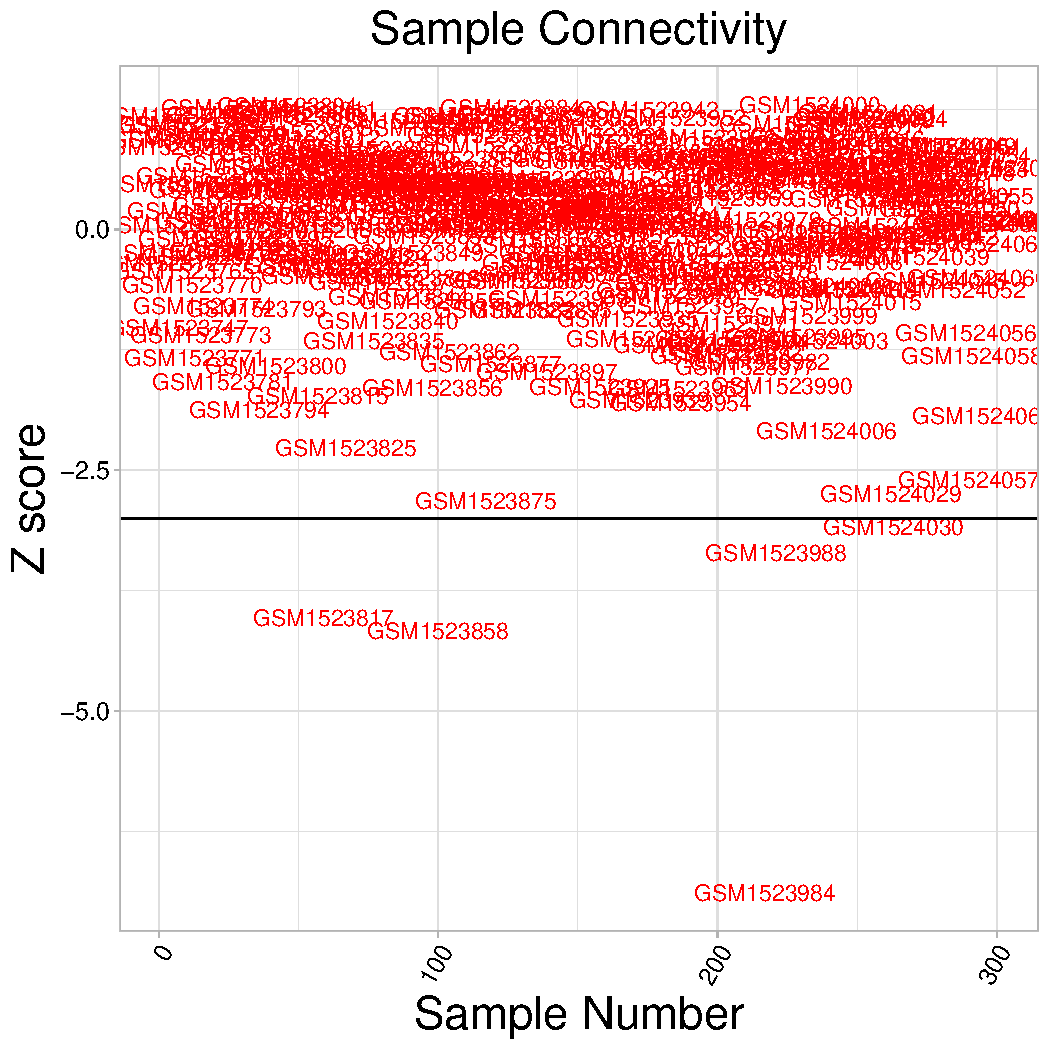
\includegraphics{tme-interactions_files/figure-latex/unnamed-chunk-8-1.pdf}

\hypertarget{deg-analysis-between-tme-subtypes}{%
\section{DEG analysis between TME subtypes}\label{deg-analysis-between-tme-subtypes}}

Identifing TME subtype-related differential genes using \texttt{find\_markers\_in\_bulk}.

We have developed a reliable classifier for the tumour microenvironment in gastric cancer using the same analysis pipeline\href{https://github.com/LiaoWJLab/TMEclassifier}{TMEclassifier}. The classifier was constructed by identifying the most robust gastric cancer TME classification through parsing the tumour microenvironment using the \texttt{tme\_cluster} method. Next, genes specifically expressed by each microenvironmental subtype are obtained using the \texttt{find\_markers\_in\_bulk\ method}. Finally, a machine learning approach was used to construct the classifier model.

\begin{Shaded}
\begin{Highlighting}[]
\FunctionTok{library}\NormalTok{(Seurat)}
\NormalTok{res }\OtherTok{\textless{}{-}} \FunctionTok{find\_markers\_in\_bulk}\NormalTok{(}\AttributeTok{pdata      =}\NormalTok{ tme, }
                            \AttributeTok{eset       =}\NormalTok{ eset, }
                            \AttributeTok{group      =} \StringTok{"cluster"}\NormalTok{, }
                            \AttributeTok{nfeatures  =} \DecValTok{2000}\NormalTok{, }
                            \AttributeTok{top\_n      =} \DecValTok{50}\NormalTok{, }
                            \AttributeTok{thresh.use =} \FloatTok{0.15}\NormalTok{, }
                            \AttributeTok{only.pos   =} \ConstantTok{TRUE}\NormalTok{, }
                            \AttributeTok{min.pct    =} \FloatTok{0.10}\NormalTok{)}
\end{Highlighting}
\end{Shaded}

\begin{verbatim}
## 
## TME3 TME2 TME1 
##  119   96   85 
## # A tibble: 150 x 7
## # Groups:   cluster [3]
##       p_val avg_log2FC pct.1 pct.2 p_val_adj cluster gene    
##       <dbl>      <dbl> <dbl> <dbl>     <dbl> <fct>   <chr>   
##  1 3.05e-22      0.896     1     1  6.63e-18 TME3    TMEM100 
##  2 7.92e-22      1.13      1     1  1.72e-17 TME3    ADH1B   
##  3 1.61e-20      0.691     1     1  3.51e-16 TME3    HHIP    
##  4 1.93e-20      0.985     1     1  4.19e-16 TME3    ABCA8   
##  5 5.73e-20      0.701     1     1  1.25e-15 TME3    FCER1A  
##  6 9.42e-19      0.927     1     1  2.05e-14 TME3    MAMDC2  
##  7 1.61e-18      0.773     1     1  3.49e-14 TME3    C1QTNF7 
##  8 1.77e-18      0.718     1     1  3.85e-14 TME3    C16orf89
##  9 3.91e-18      0.729     1     1  8.51e-14 TME3    FHL1    
## 10 5.87e-18      0.684     1     1  1.28e-13 TME3    ITGA8   
## # i 140 more rows
\end{verbatim}

\begin{Shaded}
\begin{Highlighting}[]
\NormalTok{top15 }\OtherTok{\textless{}{-}}\NormalTok{  res}\SpecialCharTok{$}\NormalTok{top\_markers }\SpecialCharTok{\%\textgreater{}\%}\NormalTok{ dplyr}\SpecialCharTok{::} \FunctionTok{group\_by}\NormalTok{(cluster) }\SpecialCharTok{\%\textgreater{}\%}\NormalTok{  dplyr}\SpecialCharTok{::}\FunctionTok{top\_n}\NormalTok{(}\DecValTok{15}\NormalTok{, avg\_log2FC)}
\NormalTok{top15}\SpecialCharTok{$}\NormalTok{gene}
\end{Highlighting}
\end{Shaded}

\begin{verbatim}
##  [1] "TMEM100"        "ADH1B"          "ABCA8"          "MAMDC2"        
##  [5] "SCN7A"          "LIPF"           "C7"             "C2orf40"       
##  [9] "PGA4"           "OGN"            "GKN2"           "GHRL"          
## [13] "C6orf58"        "SCRG1"          "GIF"            "IFNG"          
## [17] "WARS"           "CXCL10"         "IDO1"           "GZMB"          
## [21] "CXCL11"         "GBP4"           "CXCL9"          "GNLY"          
## [25] "GBP5"           "AIM2"           "RTEL1-TNFRSF6B" "COL11A1"       
## [29] "S100A2"         "SLCO1B3"        "IL1A"           "IL1B"          
## [33] "PPBP"           "IL11"           "CXCL6"          "CCL3L3"        
## [37] "TREM1"          "PROK2"          "IL24"           "PI15"          
## [41] "HCAR3"          "CLEC5A"         "MAGEA6"         "MAGEA12"       
## [45] "REG1B"
\end{verbatim}

Heatmap visualisation using \texttt{Seurat}'s \texttt{DoHeatmap}

\begin{Shaded}
\begin{Highlighting}[]
\CommentTok{\#定义分型对应的颜色}
\NormalTok{cols }\OtherTok{\textless{}{-}} \FunctionTok{c}\NormalTok{(}\StringTok{\textquotesingle{}\#2692a4\textquotesingle{}}\NormalTok{,}\StringTok{\textquotesingle{}\#fc0d3a\textquotesingle{}}\NormalTok{,}\StringTok{\textquotesingle{}\#ffbe0b\textquotesingle{}}\NormalTok{)}
\NormalTok{p1 }\OtherTok{\textless{}{-}} \FunctionTok{DoHeatmap}\NormalTok{(res}\SpecialCharTok{$}\NormalTok{sce, top15}\SpecialCharTok{$}\NormalTok{gene, }\AttributeTok{group.colors =}\NormalTok{ cols )}\SpecialCharTok{+}
  \FunctionTok{scale\_fill\_gradientn}\NormalTok{(}\AttributeTok{colours =} \FunctionTok{rev}\NormalTok{(}\FunctionTok{colorRampPalette}\NormalTok{(RColorBrewer}\SpecialCharTok{::}\FunctionTok{brewer.pal}\NormalTok{(}\DecValTok{11}\NormalTok{,}\StringTok{"RdBu"}\NormalTok{))(}\DecValTok{256}\NormalTok{)))}
\end{Highlighting}
\end{Shaded}

Extracting variables from the expression matrix to merge with TME subtype

\begin{Shaded}
\begin{Highlighting}[]
\NormalTok{input }\OtherTok{\textless{}{-}} \FunctionTok{combine\_pd\_eset}\NormalTok{(}\AttributeTok{eset =}\NormalTok{ eset, }\AttributeTok{pdata =}\NormalTok{ tme, }\AttributeTok{feas =}\NormalTok{ top15}\SpecialCharTok{$}\NormalTok{gene, }\AttributeTok{scale =}\NormalTok{ T)}
\NormalTok{p2 }\OtherTok{\textless{}{-}} \FunctionTok{sig\_box}\NormalTok{(input, }\AttributeTok{variable =} \StringTok{"cluster"}\NormalTok{, }\AttributeTok{signature =} \StringTok{"IFNG"}\NormalTok{, }\AttributeTok{jitter =} \ConstantTok{TRUE}\NormalTok{,}
              \AttributeTok{cols =}\NormalTok{  cols, }\AttributeTok{show\_pvalue =} \ConstantTok{TRUE}\NormalTok{, }\AttributeTok{size\_of\_pvalue =} \DecValTok{4}\NormalTok{)}
\end{Highlighting}
\end{Shaded}

\begin{verbatim}
## # A tibble: 3 x 8
##   .y.       group1 group2        p    p.adj p.format p.signif method  
##   <chr>     <chr>  <chr>     <dbl>    <dbl> <chr>    <chr>    <chr>   
## 1 signature TME3   TME2   1.11e-16 3.30e-16 < 2e-16  ****     Wilcoxon
## 2 signature TME3   TME1   6.70e- 1 6.7 e- 1 0.67     ns       Wilcoxon
## 3 signature TME2   TME1   5.60e-14 1.10e-13 5.6e-14  ****     Wilcoxon
\end{verbatim}

\begin{Shaded}
\begin{Highlighting}[]
\NormalTok{p3 }\OtherTok{\textless{}{-}} \FunctionTok{sig\_box}\NormalTok{(input, }\AttributeTok{variable =} \StringTok{"cluster"}\NormalTok{, }\AttributeTok{signature =} \StringTok{"IL1A"}\NormalTok{, }
              \AttributeTok{jitter =} \ConstantTok{TRUE}\NormalTok{, }\AttributeTok{cols =}\NormalTok{  cols, }\AttributeTok{show\_pvalue =} \ConstantTok{TRUE}\NormalTok{, }\AttributeTok{size\_of\_pvalue =} \DecValTok{4}\NormalTok{)}
\end{Highlighting}
\end{Shaded}

\begin{verbatim}
## # A tibble: 3 x 8
##   .y.       group1 group2        p    p.adj p.format p.signif method  
##   <chr>     <chr>  <chr>     <dbl>    <dbl> <chr>    <chr>    <chr>   
## 1 signature TME3   TME2   5.94e- 9 1.20e- 8 5.9e-09  ****     Wilcoxon
## 2 signature TME3   TME1   7.96e-18 2.40e-17 < 2e-16  ****     Wilcoxon
## 3 signature TME2   TME1   2.60e- 5 2.6 e- 5 2.6e-05  ****     Wilcoxon
\end{verbatim}

Combining the results obtained above

\begin{Shaded}
\begin{Highlighting}[]
\CommentTok{\# if (!requireNamespace("patchwork", quietly = TRUE))   install.packages("patchwork")}
\FunctionTok{library}\NormalTok{(patchwork)}
\NormalTok{p }\OtherTok{\textless{}{-}}\NormalTok{ (p1}\SpecialCharTok{|}\NormalTok{p2}\SpecialCharTok{/}\NormalTok{p3) }\SpecialCharTok{+} \FunctionTok{plot\_layout}\NormalTok{(}\AttributeTok{widths =} \FunctionTok{c}\NormalTok{(}\FloatTok{2.3}\NormalTok{,}\DecValTok{1}\NormalTok{))}
\NormalTok{p }\SpecialCharTok{+} \FunctionTok{plot\_annotation}\NormalTok{(}\AttributeTok{tag\_levels =} \StringTok{\textquotesingle{}A\textquotesingle{}}\NormalTok{)}
\end{Highlighting}
\end{Shaded}

\includegraphics{tme-interactions_files/figure-latex/unnamed-chunk-12-1.pdf}

\hypertarget{identifying-signatures-associated-with-tme-clusters}{%
\section{Identifying signatures associated with TME clusters}\label{identifying-signatures-associated-with-tme-clusters}}

Calculate TME associated signatures-(through PCA method).

\begin{Shaded}
\begin{Highlighting}[]
\NormalTok{sig\_tme}\OtherTok{\textless{}{-}}\FunctionTok{calculate\_sig\_score}\NormalTok{(}\AttributeTok{pdata           =} \ConstantTok{NULL}\NormalTok{,}
                             \AttributeTok{eset            =}\NormalTok{ eset,}
                             \AttributeTok{signature       =}\NormalTok{ signature\_collection,}
                             \AttributeTok{method          =} \StringTok{"pca"}\NormalTok{,}
                             \AttributeTok{mini\_gene\_count =} \DecValTok{2}\NormalTok{)}
\NormalTok{sig\_tme }\OtherTok{\textless{}{-}} \FunctionTok{t}\NormalTok{(}\FunctionTok{column\_to\_rownames}\NormalTok{(sig\_tme, }\AttributeTok{var =} \StringTok{"ID"}\NormalTok{))}
\NormalTok{sig\_tme[}\DecValTok{1}\SpecialCharTok{:}\DecValTok{5}\NormalTok{, }\DecValTok{1}\SpecialCharTok{:}\DecValTok{3}\NormalTok{]}
\end{Highlighting}
\end{Shaded}

\begin{verbatim}
##                   GSM1523727 GSM1523728 GSM1523729
## CD_8_T_effector   -2.5513794  0.7789141 -2.1770675
## DDR               -0.8747614  0.7425162 -1.3272054
## APM                1.1098368  2.1988688 -0.9516419
## Immune_Checkpoint -2.3701787  0.9455120 -1.4844104
## CellCycle_Reg      0.1063358  0.7583302 -0.3649795
\end{verbatim}

Finding characteristic variables associated with TME clusters

\begin{Shaded}
\begin{Highlighting}[]
\NormalTok{res }\OtherTok{\textless{}{-}} \FunctionTok{find\_markers\_in\_bulk}\NormalTok{(}\AttributeTok{pdata =}\NormalTok{ tme, }\AttributeTok{eset =}\NormalTok{ sig\_tme, }\AttributeTok{group =} \StringTok{"cluster"}\NormalTok{, }\AttributeTok{nfeatures =} \DecValTok{1000}\NormalTok{, }\AttributeTok{top\_n =} \DecValTok{20}\NormalTok{, }\AttributeTok{min.pct =} \FloatTok{0.10}\NormalTok{)}
\end{Highlighting}
\end{Shaded}

\begin{verbatim}
## 
## TME3 TME2 TME1 
##  119   96   85 
## # A tibble: 59 x 7
## # Groups:   cluster [3]
##       p_val avg_log2FC pct.1 pct.2 p_val_adj cluster gene                       
##       <dbl>      <dbl> <dbl> <dbl>     <dbl> <fct>   <chr>                      
##  1 1.05e-25       5.03 0.832 0.287  2.70e-23 TME3    Glycolysis                 
##  2 1.15e-23       3.76 0.79  0.238  2.93e-21 TME3    Tyrosine-Metabolism        
##  3 8.38e-18       4.07 0.756 0.32   2.15e-15 TME3    Drug-Metabolism-by-Cytochr~
##  4 8.59e-14       4.10 0.689 0.359  2.20e-11 TME3    Retinol-Metabolism         
##  5 2.59e-13       3.55 0.723 0.348  6.64e-11 TME3    Metabolism-of-Xenobiotics-~
##  6 5.99e-11      10.0  0.546 0.227  1.53e- 8 TME3    detox.iCAF                 
##  7 7.25e-11      10.6  0.571 0.26   1.86e- 8 TME3    Normal.Fibroblast          
##  8 2.32e-10       3.71 0.664 0.343  5.94e- 8 TME3    Ether-Lipid-Metabolism     
##  9 1.99e- 9       5.12 0.555 0.276  5.10e- 7 TME3    TMEscoreB-CIR              
## 10 2.23e- 8       3.43 0.664 0.387  5.71e- 6 TME3    Drug-Metabolism-by-other-e~
## # i 49 more rows
\end{verbatim}

\begin{Shaded}
\begin{Highlighting}[]
\NormalTok{top15 }\OtherTok{\textless{}{-}}\NormalTok{  res}\SpecialCharTok{$}\NormalTok{top\_markers }\SpecialCharTok{\%\textgreater{}\%}\NormalTok{ dplyr}\SpecialCharTok{::} \FunctionTok{group\_by}\NormalTok{(cluster) }\SpecialCharTok{\%\textgreater{}\%}\NormalTok{  dplyr}\SpecialCharTok{::}\FunctionTok{top\_n}\NormalTok{(}\DecValTok{15}\NormalTok{, avg\_log2FC)}

\NormalTok{p1 }\OtherTok{\textless{}{-}} \FunctionTok{DoHeatmap}\NormalTok{(res}\SpecialCharTok{$}\NormalTok{sce, top15}\SpecialCharTok{$}\NormalTok{gene, }\AttributeTok{group.colors =}\NormalTok{ cols)}\SpecialCharTok{+}
  \FunctionTok{scale\_fill\_gradientn}\NormalTok{(}\AttributeTok{colours =} \FunctionTok{rev}\NormalTok{(}\FunctionTok{colorRampPalette}\NormalTok{(RColorBrewer}\SpecialCharTok{::}\FunctionTok{brewer.pal}\NormalTok{(}\DecValTok{11}\NormalTok{,}\StringTok{"RdBu"}\NormalTok{))(}\DecValTok{256}\NormalTok{)))}
\end{Highlighting}
\end{Shaded}

可视化结果:选择特征变量

\begin{Shaded}
\begin{Highlighting}[]
\NormalTok{top15}\SpecialCharTok{$}\NormalTok{gene  }\OtherTok{\textless{}{-}} \FunctionTok{gsub}\NormalTok{(top15}\SpecialCharTok{$}\NormalTok{gene, }\AttributeTok{pattern =} \StringTok{"{-}"}\NormalTok{, }\AttributeTok{replacement =} \StringTok{"}\SpecialCharTok{\textbackslash{}\textbackslash{}}\StringTok{\_"}\NormalTok{)}
\NormalTok{input }\OtherTok{\textless{}{-}} \FunctionTok{combine\_pd\_eset}\NormalTok{(}\AttributeTok{eset =}\NormalTok{ sig\_tme, }\AttributeTok{pdata =}\NormalTok{ tme, }\AttributeTok{feas =}\NormalTok{ top15}\SpecialCharTok{$}\NormalTok{gene, }\AttributeTok{scale =}\NormalTok{ T)}

\NormalTok{p2 }\OtherTok{\textless{}{-}} \FunctionTok{sig\_box}\NormalTok{(input, }\AttributeTok{variable =} \StringTok{"cluster"}\NormalTok{, }\AttributeTok{signature =} \StringTok{"CD\_8\_T\_effector"}\NormalTok{, }\AttributeTok{jitter =} \ConstantTok{TRUE}\NormalTok{,}
              \AttributeTok{cols =}\NormalTok{  cols, }\AttributeTok{show\_pvalue =} \ConstantTok{TRUE}\NormalTok{, }\AttributeTok{size\_of\_pvalue =} \DecValTok{4}\NormalTok{, }\AttributeTok{size\_of\_font =} \DecValTok{6}\NormalTok{)}
\end{Highlighting}
\end{Shaded}

\begin{verbatim}
## # A tibble: 3 x 8
##   .y.       group1 group2        p    p.adj p.format p.signif method  
##   <chr>     <chr>  <chr>     <dbl>    <dbl> <chr>    <chr>    <chr>   
## 1 signature TME3   TME2   3.18e-12 6.40e-12 3.2e-12  ****     Wilcoxon
## 2 signature TME3   TME1   1.01e- 1 1   e- 1 0.1      ns       Wilcoxon
## 3 signature TME2   TME1   4.53e-13 1.4 e-12 4.5e-13  ****     Wilcoxon
\end{verbatim}

\begin{Shaded}
\begin{Highlighting}[]
\NormalTok{p3 }\OtherTok{\textless{}{-}} \FunctionTok{sig\_box}\NormalTok{(input, }\AttributeTok{variable =} \StringTok{"cluster"}\NormalTok{, }\AttributeTok{signature =} \StringTok{"Neutrophils\_Bindea\_et\_al"}\NormalTok{,  }
              \AttributeTok{jitter =} \ConstantTok{TRUE}\NormalTok{, }\AttributeTok{cols =}\NormalTok{  cols, }\AttributeTok{show\_pvalue =} \ConstantTok{TRUE}\NormalTok{, }\AttributeTok{size\_of\_pvalue =} \DecValTok{4}\NormalTok{, }\AttributeTok{size\_of\_font =} \DecValTok{6}\NormalTok{)}
\end{Highlighting}
\end{Shaded}

\begin{verbatim}
## # A tibble: 3 x 8
##   .y.       group1 group2         p    p.adj p.format p.signif method  
##   <chr>     <chr>  <chr>      <dbl>    <dbl> <chr>    <chr>    <chr>   
## 1 signature TME3   TME2   0.0000416 0.000097 4.2e-05  ****     Wilcoxon
## 2 signature TME3   TME1   0.0000323 0.000097 3.2e-05  ****     Wilcoxon
## 3 signature TME2   TME1   0.149     0.15     0.15     ns       Wilcoxon
\end{verbatim}

\begin{Shaded}
\begin{Highlighting}[]
\NormalTok{p }\OtherTok{\textless{}{-}}\NormalTok{ (p1}\SpecialCharTok{|}\NormalTok{p2}\SpecialCharTok{/}\NormalTok{p3) }\SpecialCharTok{+} \FunctionTok{plot\_layout}\NormalTok{(}\AttributeTok{widths =} \FunctionTok{c}\NormalTok{(}\FloatTok{2.3}\NormalTok{,}\DecValTok{1}\NormalTok{))}
\NormalTok{p }\SpecialCharTok{+} \FunctionTok{plot\_annotation}\NormalTok{(}\AttributeTok{tag\_levels =} \StringTok{\textquotesingle{}A\textquotesingle{}}\NormalTok{)}
\end{Highlighting}
\end{Shaded}

\includegraphics{tme-interactions_files/figure-latex/unnamed-chunk-16-1.pdf}

Survival differences between tumour microenvironment subtypes

\begin{Shaded}
\begin{Highlighting}[]
\FunctionTok{library}\NormalTok{(survminer)}
\FunctionTok{data}\NormalTok{(pdata\_acrg, }\AttributeTok{package =} \StringTok{"IOBR"}\NormalTok{)}
\NormalTok{input }\OtherTok{\textless{}{-}} \FunctionTok{merge}\NormalTok{(pdata\_acrg, input, }\AttributeTok{by =} \StringTok{"ID"}\NormalTok{)}
\NormalTok{p1}\OtherTok{\textless{}{-}}\FunctionTok{surv\_group}\NormalTok{(}\AttributeTok{input\_pdata       =}\NormalTok{ input,}
               \AttributeTok{target\_group      =} \StringTok{"cluster"}\NormalTok{,}
               \AttributeTok{ID                =} \StringTok{"ID"}\NormalTok{,}
               \AttributeTok{reference\_group   =} \StringTok{"High"}\NormalTok{,}
               \AttributeTok{project           =} \StringTok{"ACRG"}\NormalTok{,}
               \AttributeTok{cols              =}\NormalTok{ cols, }
               \AttributeTok{time              =} \StringTok{"OS\_time"}\NormalTok{,}
               \AttributeTok{status            =} \StringTok{"OS\_status"}\NormalTok{,}
               \AttributeTok{time\_type         =} \StringTok{"month"}\NormalTok{,}
               \AttributeTok{save\_path         =} \StringTok{"result"}\NormalTok{)}
\end{Highlighting}
\end{Shaded}

\begin{verbatim}
## >>> Dataset's survival follow up time is range between 1 to 105.7 months
\end{verbatim}

\begin{verbatim}
## TME1 TME2 TME3 
##   85   96  119
\end{verbatim}

\begin{verbatim}
## 8596119
\end{verbatim}

\begin{verbatim}
##   Maximum of follow up time is 105.7 months; and will be divided into 6 sections;
\end{verbatim}

\begin{Shaded}
\begin{Highlighting}[]
\NormalTok{p1}
\end{Highlighting}
\end{Shaded}

\includegraphics{tme-interactions_files/figure-latex/unnamed-chunk-17-1.pdf}

Relationship between tumour microenvironmental subtypes and other subtypes

\begin{Shaded}
\begin{Highlighting}[]
\NormalTok{p1}\OtherTok{\textless{}{-}} \FunctionTok{percent\_bar\_plot}\NormalTok{(input, }\AttributeTok{x =} \StringTok{"cluster"}\NormalTok{ , }\AttributeTok{y =} \StringTok{"Subtype"}\NormalTok{, }\AttributeTok{palette =} \StringTok{"jama"}\NormalTok{, }\AttributeTok{axis\_angle =} \DecValTok{60}\NormalTok{)}
\end{Highlighting}
\end{Shaded}

\begin{verbatim}
## # A tibble: 12 x 5
## # Groups:   cluster [3]
##    cluster Subtype    Freq  Prop count
##    <chr>   <fct>     <dbl> <dbl> <dbl>
##  1 TME1    EMT          14  0.16    85
##  2 TME1    MSI          12  0.14    85
##  3 TME1    MSS/TP53-    34  0.4     85
##  4 TME1    MSS/TP53+    25  0.29    85
##  5 TME2    EMT           6  0.06    96
##  6 TME2    MSI          47  0.49    96
##  7 TME2    MSS/TP53-    22  0.23    96
##  8 TME2    MSS/TP53+    21  0.22    96
##  9 TME3    EMT          26  0.22   119
## 10 TME3    MSI           9  0.08   119
## 11 TME3    MSS/TP53-    51  0.43   119
## 12 TME3    MSS/TP53+    33  0.28   119
## [1] "'#374E55FF', '#DF8F44FF', '#00A1D5FF', '#B24745FF', '#79AF97FF', '#6A6599FF', '#80796BFF'"
\end{verbatim}

\begin{Shaded}
\begin{Highlighting}[]
\NormalTok{p2}\OtherTok{\textless{}{-}} \FunctionTok{percent\_bar\_plot}\NormalTok{(input, }\AttributeTok{x =} \StringTok{"cluster"}\NormalTok{ , }\AttributeTok{y =} \StringTok{"Lauren"}\NormalTok{, }\AttributeTok{palette =} \StringTok{"jama"}\NormalTok{, }\AttributeTok{axis\_angle =} \DecValTok{60}\NormalTok{)}
\end{Highlighting}
\end{Shaded}

\begin{verbatim}
## # A tibble: 9 x 5
## # Groups:   cluster [3]
##   cluster Lauren      Freq  Prop count
##   <chr>   <fct>      <dbl> <dbl> <dbl>
## 1 TME1    Diffuse       37  0.44    85
## 2 TME1    Intestinal    47  0.55    85
## 3 TME1    Mixed          1  0.01    85
## 4 TME2    Diffuse       31  0.32    96
## 5 TME2    Intestinal    54  0.56    96
## 6 TME2    Mixed         11  0.11    96
## 7 TME3    Diffuse       67  0.56   119
## 8 TME3    Intestinal    45  0.38   119
## 9 TME3    Mixed          7  0.06   119
## [1] "'#374E55FF', '#DF8F44FF', '#00A1D5FF', '#B24745FF', '#79AF97FF', '#6A6599FF', '#80796BFF'"
\end{verbatim}

\begin{Shaded}
\begin{Highlighting}[]
\NormalTok{p3}\OtherTok{\textless{}{-}} \FunctionTok{percent\_bar\_plot}\NormalTok{(input, }\AttributeTok{x =} \StringTok{"cluster"}\NormalTok{ , }\AttributeTok{y =} \StringTok{"TMEscore\_binary"}\NormalTok{, }\AttributeTok{palette =} \StringTok{"jama"}\NormalTok{, }\AttributeTok{axis\_angle =} \DecValTok{60}\NormalTok{)}
\end{Highlighting}
\end{Shaded}

\begin{verbatim}
## # A tibble: 7 x 5
## # Groups:   cluster [3]
##   cluster TMEscore_binary  Freq  Prop count
##   <chr>   <fct>           <dbl> <dbl> <dbl>
## 1 TME1    High                5  0.06    85
## 2 TME1    Low                79  0.93    85
## 3 TME1    <NA>                1  0.01    85
## 4 TME2    High               59  0.61    96
## 5 TME2    Low                37  0.39    96
## 6 TME3    High                7  0.06   119
## 7 TME3    Low               112  0.94   119
## [1] "'#374E55FF', '#DF8F44FF', '#00A1D5FF', '#B24745FF', '#79AF97FF', '#6A6599FF', '#80796BFF'"
\end{verbatim}

\begin{Shaded}
\begin{Highlighting}[]
\NormalTok{p1}\SpecialCharTok{|}\NormalTok{p2}\SpecialCharTok{|}\NormalTok{p3}
\end{Highlighting}
\end{Shaded}

\includegraphics{tme-interactions_files/figure-latex/unnamed-chunk-19-1.pdf}

\hypertarget{references-3}{%
\section{References}\label{references-3}}

Cristescu, R., Lee, J., Nebozhyn, M. et al.~Molecular analysis of gastric cancer identifies subtypes associated with distinct clinical outcomes. Nat Med 21, 449--456 (2015). \url{https://doi.org/10.1038/nm.3850}

\href{https://cibersort.stanford.edu/}{CIBERSORT}; Newman, A. M., Liu, C. L., Green, M. R., Gentles, A. J., Feng, W., Xu, Y., \ldots{} Alizadeh, A. A. (2015). Robust enumeration of cell subsets from tissue expression profiles. Nature Methods, 12(5), 453--457. \url{https://doi.org/10.1038/nmeth.3337};

Seurat: Hao and Hao et al.~Integrated analysis of multimodal single-cell data. Cell (2021)

\hypertarget{tumor-ecosystem-analysis}{%
\chapter{\texorpdfstring{\textbf{Tumor ecosystem analysis}}{Tumor ecosystem analysis}}\label{tumor-ecosystem-analysis}}

\hypertarget{loading-packages-5}{%
\section{Loading packages}\label{loading-packages-5}}

\begin{Shaded}
\begin{Highlighting}[]
\FunctionTok{library}\NormalTok{(IOBR)}
\end{Highlighting}
\end{Shaded}

\hypertarget{downloading-data-for-example-4}{%
\section{Downloading data for example}\label{downloading-data-for-example-4}}

Obtaining data set from GEO \href{https://pubmed.ncbi.nlm.nih.gov/25894828/}{Gastric cancer: GSE62254} using \texttt{GEOquery} R package.

\begin{Shaded}
\begin{Highlighting}[]
\ControlFlowTok{if}\NormalTok{ (}\SpecialCharTok{!}\FunctionTok{requireNamespace}\NormalTok{(}\StringTok{"GEOquery"}\NormalTok{, }\AttributeTok{quietly =} \ConstantTok{TRUE}\NormalTok{))  BiocManager}\SpecialCharTok{::}\FunctionTok{install}\NormalTok{(}\StringTok{"GEOquery"}\NormalTok{)}
\FunctionTok{library}\NormalTok{(}\StringTok{"GEOquery"}\NormalTok{)}
\CommentTok{\# }\AlertTok{NOTE}\CommentTok{: This process may take a few minutes which depends on the internet connection speed. Please wait for its completion.}
\NormalTok{eset\_geo}\OtherTok{\textless{}{-}}\FunctionTok{getGEO}\NormalTok{(}\AttributeTok{GEO     =} \StringTok{"GSE62254"}\NormalTok{, }\AttributeTok{getGPL  =}\NormalTok{ F, }\AttributeTok{destdir =} \StringTok{"./"}\NormalTok{)}
\NormalTok{eset    }\OtherTok{\textless{}{-}}\NormalTok{eset\_geo[[}\DecValTok{1}\NormalTok{]]}
\NormalTok{eset    }\OtherTok{\textless{}{-}}\FunctionTok{exprs}\NormalTok{(eset)}
\NormalTok{eset[}\DecValTok{1}\SpecialCharTok{:}\DecValTok{5}\NormalTok{,}\DecValTok{1}\SpecialCharTok{:}\DecValTok{5}\NormalTok{]}
\end{Highlighting}
\end{Shaded}

\begin{verbatim}
##           GSM1523727 GSM1523728 GSM1523729 GSM1523744 GSM1523745
## 1007_s_at  3.2176645  3.0624323  3.0279131   2.921683  2.8456013
## 1053_at    2.4050109  2.4394879  2.2442708   2.345916  2.4328582
## 117_at     1.4933412  1.8067380  1.5959665   1.839822  1.8326058
## 121_at     2.1965561  2.2812181  2.1865556   2.258599  2.1874363
## 1255_g_at  0.8698382  0.9502466  0.8125414   1.012860  0.9441993
\end{verbatim}

\hypertarget{gene-annotation-hgu133plus-2-affaymetrix-1}{%
\section{Gene Annotation: HGU133PLUS-2 (Affaymetrix)}\label{gene-annotation-hgu133plus-2-affaymetrix-1}}

\begin{Shaded}
\begin{Highlighting}[]
\CommentTok{\# Conduct gene annotation using \textasciigrave{}anno\_hug133plus2\textasciigrave{} file; If identical gene symbols exists, these genes would be ordered by the mean expression levels. The gene symbol with highest mean expression level is selected and remove others. }

\NormalTok{eset}\OtherTok{\textless{}{-}}\FunctionTok{anno\_eset}\NormalTok{(}\AttributeTok{eset       =}\NormalTok{ eset,}
                \AttributeTok{annotation =}\NormalTok{ anno\_hug133plus2,}
                \AttributeTok{symbol     =} \StringTok{"symbol"}\NormalTok{,}
                \AttributeTok{probe      =} \StringTok{"probe\_id"}\NormalTok{,}
                \AttributeTok{method     =} \StringTok{"mean"}\NormalTok{)}
\NormalTok{eset[}\DecValTok{1}\SpecialCharTok{:}\DecValTok{5}\NormalTok{, }\DecValTok{1}\SpecialCharTok{:}\DecValTok{3}\NormalTok{]}
\end{Highlighting}
\end{Shaded}

\begin{verbatim}
##              GSM1523727 GSM1523728 GSM1523729
## SH3KBP1        4.327974   4.316195   4.351425
## RPL41          4.246149   4.246808   4.257940
## EEF1A1         4.293762   4.291038   4.262199
## COX2           4.250288   4.283714   4.270508
## LOC101928826   4.219303   4.219670   4.213252
\end{verbatim}

\hypertarget{determine-tme-subtype-of-gastric-cancer-using-tmeclassifier-r-package}{%
\section{\texorpdfstring{Determine TME subtype of gastric cancer using \href{https://github.com/LiaoWJLab/TMEclassifier}{TMEclassifier R package}}{Determine TME subtype of gastric cancer using TMEclassifier R package}}\label{determine-tme-subtype-of-gastric-cancer-using-tmeclassifier-r-package}}

\begin{Shaded}
\begin{Highlighting}[]
\ControlFlowTok{if}\NormalTok{ (}\SpecialCharTok{!}\FunctionTok{requireNamespace}\NormalTok{(}\StringTok{"TMEclassifier"}\NormalTok{, }\AttributeTok{quietly =} \ConstantTok{TRUE}\NormalTok{)) devtools}\SpecialCharTok{::}\FunctionTok{install\_github}\NormalTok{(}\StringTok{"LiaoWJLab/TMEclassifier"}\NormalTok{)}
\FunctionTok{library}\NormalTok{(TMEclassifier)}
\NormalTok{tme }\OtherTok{\textless{}{-}} \FunctionTok{tme\_classifier}\NormalTok{(}\AttributeTok{eset =}\NormalTok{ eset, }\AttributeTok{scale =} \ConstantTok{TRUE}\NormalTok{)}
\end{Highlighting}
\end{Shaded}

\begin{verbatim}
## Step-1: Expression data preprocessing...
## Step-2: TME deconvolution...
## Step-3: Predicting TME phenotypes...
## [20:18:26] WARNING: src/learner.cc:1203: 
##   If you are loading a serialized model (like pickle in Python, RDS in R) generated by
##   older XGBoost, please export the model by calling `Booster.save_model` from that version
##   first, then load it back in current version. See:
## 
##     https://xgboost.readthedocs.io/en/latest/tutorials/saving_model.html
## 
##   for more details about differences between saving model and serializing.
## 
## [20:18:26] WARNING: src/learner.cc:888: Found JSON model saved before XGBoost 1.6, please save the model using current version again. The support for old JSON model will be discontinued in XGBoost 2.3.
## [20:18:26] WARNING: src/learner.cc:553: 
##   If you are loading a serialized model (like pickle in Python, RDS in R) generated by
##   older XGBoost, please export the model by calling `Booster.save_model` from that version
##   first, then load it back in current version. See:
## 
##     https://xgboost.readthedocs.io/en/latest/tutorials/saving_model.html
## 
##   for more details about differences between saving model and serializing.
## 
## >>>--- DONE!
\end{verbatim}

\begin{Shaded}
\begin{Highlighting}[]
\FunctionTok{table}\NormalTok{(tme}\SpecialCharTok{$}\NormalTok{TMEcluster)}
\end{Highlighting}
\end{Shaded}

\begin{verbatim}
## 
##  IA  IE  IS 
## 107  96  97
\end{verbatim}

\begin{Shaded}
\begin{Highlighting}[]
\FunctionTok{head}\NormalTok{(tme)}
\end{Highlighting}
\end{Shaded}

\begin{verbatim}
##           ID          IE         IS         IA TMEcluster
## 1 GSM1523727 0.204623557 0.11212681 0.68324962         IA
## 2 GSM1523728 0.009599504 0.11179146 0.87860903         IA
## 3 GSM1523729 0.852615046 0.11369089 0.03369407         IE
## 4 GSM1523744 0.053842233 0.06994632 0.87621145         IA
## 5 GSM1523745 0.055973019 0.80839488 0.13563209         IS
## 6 GSM1523746 0.545343299 0.37437568 0.08028102         IE
\end{verbatim}

\begin{Shaded}
\begin{Highlighting}[]
\FunctionTok{table}\NormalTok{(tme}\SpecialCharTok{$}\NormalTok{TMEcluster)}
\end{Highlighting}
\end{Shaded}

\begin{verbatim}
## 
##  IA  IE  IS 
## 107  96  97
\end{verbatim}

\begin{Shaded}
\begin{Highlighting}[]
\FunctionTok{head}\NormalTok{(tme)}
\end{Highlighting}
\end{Shaded}

\begin{verbatim}
##           ID          IE         IS         IA TMEcluster
## 1 GSM1523727 0.204623557 0.11212681 0.68324962         IA
## 2 GSM1523728 0.009599504 0.11179146 0.87860903         IA
## 3 GSM1523729 0.852615046 0.11369089 0.03369407         IE
## 4 GSM1523744 0.053842233 0.06994632 0.87621145         IA
## 5 GSM1523745 0.055973019 0.80839488 0.13563209         IS
## 6 GSM1523746 0.545343299 0.37437568 0.08028102         IE
\end{verbatim}

\hypertarget{deg-analysis-method1}{%
\section{DEG analysis: method1}\label{deg-analysis-method1}}

Differential analysis of selected immune-activated and immune-expelled gastric cancers

\begin{Shaded}
\begin{Highlighting}[]
\NormalTok{pdata }\OtherTok{\textless{}{-}}\NormalTok{ tme[}\SpecialCharTok{!}\NormalTok{tme}\SpecialCharTok{$}\NormalTok{TMEcluster}\SpecialCharTok{==}\StringTok{"IS"}\NormalTok{, ]}
\NormalTok{deg  }\OtherTok{\textless{}{-}}   \FunctionTok{iobr\_deg}\NormalTok{(}\AttributeTok{eset         =}\NormalTok{ eset,}
                   \AttributeTok{annotation    =} \ConstantTok{NULL}\NormalTok{,}
                   \AttributeTok{pdata        =}\NormalTok{ pdata,}
                   \AttributeTok{group\_id     =} \StringTok{"TMEcluster"}\NormalTok{,}
                   \AttributeTok{pdata\_id     =} \StringTok{"ID"}\NormalTok{,}
                   \AttributeTok{array        =} \ConstantTok{TRUE}\NormalTok{,}
                   \AttributeTok{method       =} \StringTok{"limma"}\NormalTok{,}
                   \AttributeTok{contrast     =} \FunctionTok{c}\NormalTok{(}\StringTok{"IA"}\NormalTok{,}\StringTok{"IE"}\NormalTok{),}
                   \AttributeTok{path         =} \StringTok{"result"}\NormalTok{,}
                   \AttributeTok{padj\_cutoff  =} \FloatTok{0.01}\NormalTok{,}
                   \AttributeTok{logfc\_cutoff =} \FloatTok{0.5}\NormalTok{)}
\end{Highlighting}
\end{Shaded}

\begin{verbatim}
## >>>== Matching grouping information and expression matrix
\end{verbatim}

\begin{verbatim}
## >>>== limma was selected for differential gene analysis of Array data
\end{verbatim}

\begin{verbatim}
## Warning: package 'limma' was built under R version 4.2.1
\end{verbatim}

\begin{verbatim}
## 
## Attaching package: 'limma'
\end{verbatim}

\begin{verbatim}
## The following object is masked from 'package:BiocGenerics':
## 
##     plotMA
\end{verbatim}

\begin{verbatim}
## group1 = IE
\end{verbatim}

\begin{verbatim}
## group2 = NA
\end{verbatim}

\begin{verbatim}
## # A tibble: 6 x 11
##   symbol  log2FoldChange AveExpr     t   pvalue     padj     B sigORnot    label
##   <chr>            <dbl>   <dbl> <dbl>    <dbl>    <dbl> <dbl> <chr>       <chr>
## 1 TMEM100          0.774    1.84  13.9 2.47e-31 5.37e-27  60.4 Up_regulat~ Both 
## 2 ABCA8            0.933    1.90  12.9 3.11e-28 3.38e-24  53.4 Up_regulat~ Both 
## 3 HHIP             0.613    1.73  12.1 7.62e-26 4.46e-22  48.0 Up_regulat~ Both 
## 4 LMNB2           -0.287    2.25 -12.1 9.28e-26 4.46e-22  47.8 NOT         Sign~
## 5 MCM6            -0.211    3.02 -12.1 1.02e-25 4.46e-22  47.7 NOT         Sign~
## 6 ADH1B            0.907    1.86  12.0 2.27e-25 7.04e-22  47.0 Up_regulat~ Both 
## # i 2 more variables: IE <dbl>, `` <dbl>
\end{verbatim}

\hypertarget{gsea-analysis-based-on-differential-express-gene-analysis-results}{%
\section{GSEA analysis based on differential express gene analysis results}\label{gsea-analysis-based-on-differential-express-gene-analysis-results}}

Select the gene set list in IOBR's signature collection.

\begin{Shaded}
\begin{Highlighting}[]
\FunctionTok{head}\NormalTok{(deg)}
\end{Highlighting}
\end{Shaded}

\begin{verbatim}
## # A tibble: 6 x 11
##   symbol  log2FoldChange AveExpr     t   pvalue     padj     B sigORnot    label
##   <chr>            <dbl>   <dbl> <dbl>    <dbl>    <dbl> <dbl> <chr>       <chr>
## 1 TMEM100          0.774    1.84  13.9 2.47e-31 5.37e-27  60.4 Up_regulat~ Both 
## 2 ABCA8            0.933    1.90  12.9 3.11e-28 3.38e-24  53.4 Up_regulat~ Both 
## 3 HHIP             0.613    1.73  12.1 7.62e-26 4.46e-22  48.0 Up_regulat~ Both 
## 4 LMNB2           -0.287    2.25 -12.1 9.28e-26 4.46e-22  47.8 NOT         Sign~
## 5 MCM6            -0.211    3.02 -12.1 1.02e-25 4.46e-22  47.7 NOT         Sign~
## 6 ADH1B            0.907    1.86  12.0 2.27e-25 7.04e-22  47.0 Up_regulat~ Both 
## # i 2 more variables: IE <dbl>, `` <dbl>
\end{verbatim}

\begin{Shaded}
\begin{Highlighting}[]
\NormalTok{sig\_list }\OtherTok{\textless{}{-}}\NormalTok{ signature\_collection[}\FunctionTok{c}\NormalTok{(}\StringTok{"TMEscoreB\_CIR"}\NormalTok{, }\StringTok{"TMEscoreA\_CIR"}\NormalTok{, }\StringTok{"DNA\_replication"}\NormalTok{, }\StringTok{"Base\_excision\_repair"}\NormalTok{,}
                                   \StringTok{"Pan\_F\_TBRs"}\NormalTok{, }\StringTok{"TGFb.myCAF"}\NormalTok{, }\StringTok{"Ferroptosis"}\NormalTok{, }\StringTok{"TLS\_Nature"}\NormalTok{, }\StringTok{"Glycolysis"}\NormalTok{)]}
\NormalTok{sig\_list}
\end{Highlighting}
\end{Shaded}

\begin{verbatim}
## $TMEscoreB_CIR
##   [1] "DCN"          "SEPP1"        "ACTA2"        "SPARCL1"      "BEX3"        
##   [6] "MYLK"         "AKR1C1"       "TIMP2"        "MXRA7"        "C11orf96"    
##  [11] "CAV1"         "PDGFRA"       "FHL1"         "MGP"          "EID1"        
##  [16] "LOC101930400" "DST"          "GREM1"        "FERMT2"       "TNC"         
##  [21] "CYBRD1"       "LTBP1"        "ACTG2"        "TMEM47"       "SERPINE2"    
##  [26] "ANTXR2"       "GNG11"        "TAGLN"        "GSTA4"        "PKIG"        
##  [31] "MAOA"         "PTRF"         "FAM3B"        "PBX1"         "WLS"         
##  [36] "SELM"         "SVIL"         "MYH11"        "AGT"          "SPON1"       
##  [41] "TGFB1I1"      "PDLIM3"       "PDK4"         "SYNPO2"       "MSRB3"       
##  [46] "PROS1"        "EDNRA"        "AKAP12"       "PSD3"         "TNS1"        
##  [51] "JAM3"         "PDZRN3"       "DDR2"         "HMGCS2"       "SGCE"        
##  [56] "MRVI1"        "WFDC1"        "FBLN1"        "FMO5"         "MAOB"        
##  [61] "AMOTL1"       "AKT3"         "CNRIP1"       "CPE"          "MAP1B"       
##  [66] "RBP1"         "GNAI1"        "FOXF2"        "SORBS2"       "ZCCHC24"     
##  [71] "ZNF704"       "ARMCX1"       "DIXDC1"       "SSTR1"        "THRB"        
##  [76] "C3orf70"      "PKIB"         "CNN1"         "SYTL5"        "DACT1"       
##  [81] "SYNPO"        "GAS1"         "DPYSL3"       "CCDC80"       "TSPYL5"      
##  [86] "DCHS1"        "SOBP"         "AOC3"         "NDN"          "FGF7P3"      
##  [91] "SMAD9"        "MCC"          "CLMP"         "MYL9"         "RBP4"        
##  [96] "PLN"          "SPOCK1"       "COL14A1"      "CRYAB"        "SRPX"        
## [101] "EML1"         "RERG"         "PPP1R3C"      "LOC100506718" "CH25H"       
## [106] "HSPB8"        "PID1"         "TTC28"        "STON1"        "ABCG2"       
## [111] "ZSCAN18"      "SCIN"         "C14orf132"    "TMEM55A"      "WASF3"       
## [116] "PAPLN"        "COLEC12"      "ACKR1"        "TMEM150C"     "RAI2"        
## [121] "TSPAN7"       "MRGPRF"       "ABCA8"        "CHIC1"        "NBEA"        
## [126] "FAM13C"       "SETBP1"       "LDOC1"        "TMEM100"      "LOC101930349"
## [131] "PRICKLE2"     "TSPAN18"      "FABP4"        "ARHGEF26"     "ERICH5"      
## [136] "MYOCD"        "BEX2"         "PPP1R14A"     "FGF13"        "RUNX1T1"     
## [141] "MAGI2-AS3"    "LINC01279"    "REEP1"        "PLAC9"        "MYEF2"       
## [146] "PRKD1"        "RGN"          "CLDN11"       "ANK2"         "ESRRG"       
## [151] "SYNC"         "ZNF667-AS1"   "FGF7"         "SFRP1"        "HMCN1"       
## [156] "TCEAL7"       "OGN"          "MAGI2"        "MIR100HG"     "FILIP1"      
## [161] "LOC100507334" "ANKRD6"       "PLEKHH2"      "ZNF542P"      "ARMCX4"      
## [166] "NOV"          "DCLK1"        "ARHGAP28"     "C2orf40"      "TRHDE"       
## [171] "EPHA7"        "SCRG1"        "ZNF677"       "ZFPM2"        "PEG3"        
## [176] "SERP2"        "ZNF415"       "MAMDC2"       "RBM24"        "MEOX2"       
## 
## $TMEscoreA_CIR
##  [1] "HLA-DPB1"       "UBD"            "LOC100509457"   "WARS"          
##  [5] "TAP1"           "HLA-DMA"        "TRIM22"         "PSAT1"         
##  [9] "CXCL10"         "SOCS3"          "CXCL9"          "PBK"           
## [13] "CCL4"           "CCL5"           "BCL2A1"         "TRBC1"         
## [17] "IDO1"           "NFE2L3"         "CCL3L3"         "DTL"           
## [21] "MMP9"           "SLC2A3"         "ZNF367"         "RCC1"          
## [25] "STIL"           "TRAC"           "HELLS"          "GZMB"          
## [29] "RTEL1-TNFRSF6B" "CXCL11"         "GBP5"           "CD2"           
## [33] "CDCA2"          "CDT1"           "TNFAIP2"        "TYMP"          
## [37] "MICB"           "SLC2A14"        "GZMK"           "CD8A"          
## [41] "CENPH"          "MND1"           "BATF2"          "BRIP1"         
## [45] "E2F7"           "KIF18A"         "AIM2"           "ETV7"          
## [49] "ITK"            "GNLY"           "GPR171"         "WDHD1"         
## [53] "GBP4"           "MB21D1"         "NLRP3"          "MCEMP1"        
## [57] "POLR3G"         "NLRC3"          "KLRC2"          "CLEC5A"        
## [61] "ARHGAP11A"      "GPR84"          "IFNG"           "ZBED2"         
## 
## $DNA_replication
##  [1] "RNASEH2A" "POLD3"    "DNA2"     "FEN1"     "POLA2"    "RNASEH1" 
##  [7] "RPA4"     "LIG1"     "MCM2"     "MCM3"     "MCM4"     "MCM5"    
## [13] "MCM6"     "MCM7"     "PCNA"     "POLE3"    "POLA1"    "POLD1"   
## [19] "POLD2"    "POLE"     "POLE2"    "PRIM1"    "PRIM2"    "POLE4"   
## [25] "POLD4"    "RFC1"     "RFC2"     "RFC3"     "RFC4"     "RFC5"    
## [31] "RPA1"     "RPA2"     "RPA3"     "SSBP1"    "RNASEH2B" "RNASEH2C"
## 
## $Base_excision_repair
##  [1] "PARP2" "PARP3" "POLD3" "PARP1" "PARP4" "FEN1"  "SMUG1" "NEIL2" "APEX2"
## [10] "POLL"  "HMGB1" "APEX1" "LIG1"  "LIG3"  "MPG"   "MUTYH" "NTHL1" "OGG1" 
## [19] "PCNA"  "POLE3" "POLB"  "POLD1" "POLD2" "POLE"  "POLE2" "NEIL3" "POLE4"
## [28] "POLD4" "UNG"   "XRCC1" "NEIL1" "MBD4" 
## 
## $Pan_F_TBRs
##  [1] "ACTA2"    "ACTG2"    "ADAM12"   "ADAM19"   "CNN1"     "COL4A1"  
##  [7] "CTGF"     "CTPS1"    "FAM101B"  "FSTL3"    "HSPB1"    "IGFBP3"  
## [13] "PXDC1"    "SEMA7A"   "SH3PXD2A" "TAGLN"    "TGFBI"    "TNS1"    
## [19] "TPM1"    
## 
## $TGFb.myCAF
##  [1] "CST1"    "LAMP5"   "LOXL1"   "EDNRA"   "TGFB1"   "TGFB3"   "TNN"    
##  [8] "CST2"    "HES4"    "COL10A1" "ELN"     "THBS4"   "NKD2"    "OLFM2"  
## [15] "COL6A3"  "LRRC17"  "COL3A1"  "THY1"    "HTRA3"   "TMEM204" "11-Sep" 
## [22] "COMP"    "TNFAIP6" "ID4"     "GGT5"    "INAFM1"  "CILP"    "OLFML2B"
## 
## $Ferroptosis
##  [1] "ACSL4"      "AKR1C1-3"   "ALOXs"      "ATP5G3"     "CARS"      
##  [6] "CBS"        "CD44v"      "CHAC1"      "CISD1"      "CS"        
## [11] "DPP4"       "FANCD2"     "GCLC/GCLM"  "GLS2"       "GPX4"      
## [16] "GSS"        "HMGCR"      "HSPB1/5"    "KOD"        "LPCAT3"    
## [21] "MT1G"       "NCOA4"      "NFE2L2"     "PTGS2"      "RPL8"      
## [26] "SAT1"       "SLC7A11"    "SQS"        "TFRC"       "TP53"      
## [31] "TTC35/EMC2" "MESH1"     
## 
## $TLS_Nature
## [1] "CD79B"  "CD1D"   "CCR6"   "LAT"    "SKAP1"  "CETP"   "EIF1AY" "RBP5"  
## [9] "PTGDS" 
## 
## $Glycolysis
##  [1] "ACSS1"   "ACSS2"   "ADH1A"   "ADH1B"   "ADH1C"   "ADH4"    "ADH5"   
##  [8] "ADH6"    "ADH7"    "ADPGK"   "AKR1A1"  "ALDH1A3" "ALDH1B1" "ALDH2"  
## [15] "ALDH3A1" "ALDH3A2" "ALDH3B1" "ALDH3B2" "ALDH7A1" "ALDH9A1" "ALDOA"  
## [22] "ALDOB"   "ALDOC"   "BPGM"    "DLAT"    "DLD"     "ENO1"    "ENO2"   
## [29] "ENO3"    "FBP1"    "FBP2"    "G6PC"    "G6PC2"   "GALM"    "GAPDH"  
## [36] "GAPDHS"  "GCK"     "GPI"     "HK1"     "HK2"     "HK3"     "HKDC1"  
## [43] "LDHA"    "LDHAL6A" "LDHAL6B" "LDHB"    "LDHC"    "PANK1"   "PCK1"   
## [50] "PCK2"    "PDHA1"   "PDHA2"   "PDHB"    "PFKFB1"  "PFKFB2"  "PFKFB3" 
## [57] "PFKFB4"  "PFKL"    "PFKM"    "PFKP"    "PGAM1"   "PGAM2"   "PGAM4"  
## [64] "PGK1"    "PGK2"    "PGM1"    "PGM2"    "PKLR"    "PKM"     "SLC2A2" 
## [71] "TPI1"
\end{verbatim}

\begin{Shaded}
\begin{Highlighting}[]
\NormalTok{gsea}\OtherTok{\textless{}{-}}     \FunctionTok{sig\_gsea}\NormalTok{(deg,}
                    \AttributeTok{genesets          =}\NormalTok{ sig\_list,}
                    \AttributeTok{path              =} \StringTok{"result"}\NormalTok{,}
                    \AttributeTok{gene\_symbol       =} \StringTok{"symbol"}\NormalTok{,}
                    \AttributeTok{logfc             =} \StringTok{"log2FoldChange"}\NormalTok{,}
                    \AttributeTok{org               =} \StringTok{"hsa"}\NormalTok{,}
                    \AttributeTok{show\_plot         =} \ConstantTok{FALSE}\NormalTok{,}
                    \AttributeTok{msigdb            =} \ConstantTok{TRUE}\NormalTok{,}
                    \AttributeTok{category          =} \StringTok{"H"}\NormalTok{,}
                    \AttributeTok{subcategory       =} \ConstantTok{NULL}\NormalTok{,}
                    \AttributeTok{palette\_bar       =} \StringTok{"set2"}\NormalTok{)}
\end{Highlighting}
\end{Shaded}

\begin{figure}

{\centering 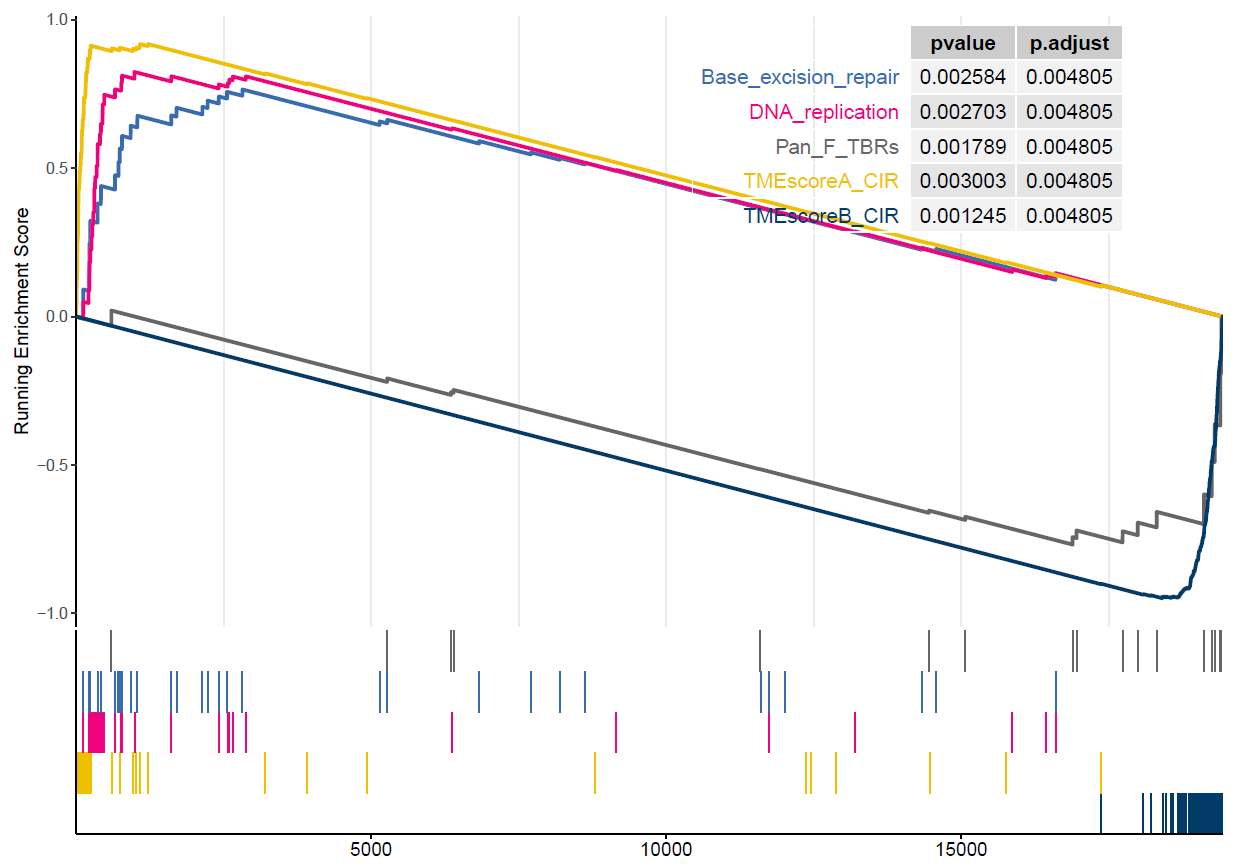
\includegraphics[width=0.95\linewidth]{./fig/gsea-1} 

}

\caption{GSEA of TME gent sets}\label{fig:unnamed-chunk-9}
\end{figure}

Hallmark gene signatures

\begin{Shaded}
\begin{Highlighting}[]
\NormalTok{gsea}\OtherTok{\textless{}{-}}     \FunctionTok{sig\_gsea}\NormalTok{(deg,}
                    \AttributeTok{genesets          =} \ConstantTok{NULL}\NormalTok{,}
                    \AttributeTok{path              =} \StringTok{"GSEA"}\NormalTok{,}
                    \AttributeTok{gene\_symbol       =} \StringTok{"symbol"}\NormalTok{,}
                    \AttributeTok{logfc             =} \StringTok{"log2FoldChange"}\NormalTok{,}
                    \AttributeTok{org               =} \StringTok{"hsa"}\NormalTok{,}
                    \AttributeTok{show\_plot         =} \ConstantTok{FALSE}\NormalTok{,}
                    \AttributeTok{msigdb            =} \ConstantTok{TRUE}\NormalTok{,}
                    \AttributeTok{category          =} \StringTok{"H"}\NormalTok{,}
                    \AttributeTok{subcategory       =} \ConstantTok{NULL}\NormalTok{,}
                    \AttributeTok{palette\_bar       =} \StringTok{"aaas"}\NormalTok{,}
                    \AttributeTok{show\_bar          =} \DecValTok{5}\NormalTok{,}
                    \AttributeTok{show\_gsea         =} \DecValTok{6}\NormalTok{)}
\end{Highlighting}
\end{Shaded}

\begin{figure}

{\centering 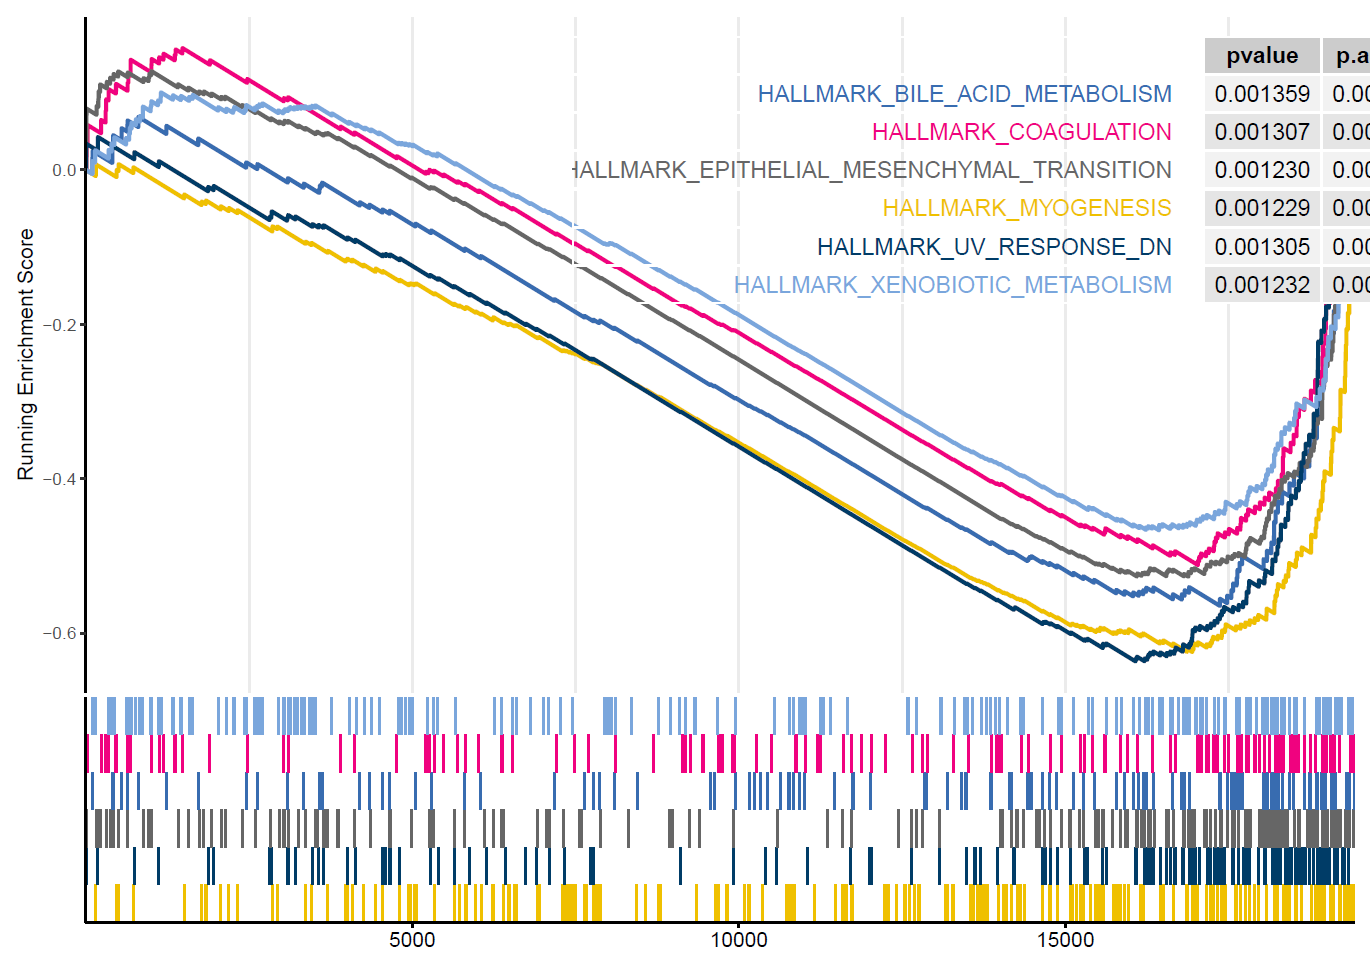
\includegraphics[width=0.95\linewidth]{./fig/gsea-2} 

}

\caption{GSEA of Hallmark gent sets}\label{fig:unnamed-chunk-11}
\end{figure}

\hypertarget{deg-analysis-method2}{%
\section{DEG analysis: method2}\label{deg-analysis-method2}}

Identifing TME subtype-related differential genes using \texttt{find\_markers\_in\_bulk}

\begin{Shaded}
\begin{Highlighting}[]
\FunctionTok{library}\NormalTok{(Seurat)}
\NormalTok{res }\OtherTok{\textless{}{-}} \FunctionTok{find\_markers\_in\_bulk}\NormalTok{(}\AttributeTok{pdata      =}\NormalTok{ tme, }
                            \AttributeTok{eset       =}\NormalTok{ eset, }
                            \AttributeTok{group      =} \StringTok{"TMEcluster"}\NormalTok{, }
                            \AttributeTok{nfeatures  =} \DecValTok{2000}\NormalTok{, }
                            \AttributeTok{top\_n      =} \DecValTok{50}\NormalTok{, }
                            \AttributeTok{thresh.use =} \FloatTok{0.15}\NormalTok{, }
                            \AttributeTok{only.pos   =} \ConstantTok{TRUE}\NormalTok{, }
                            \AttributeTok{min.pct    =} \FloatTok{0.10}\NormalTok{)}
\end{Highlighting}
\end{Shaded}

\begin{verbatim}
## 
##  IA  IE  IS 
## 107  96  97 
## # A tibble: 150 x 7
## # Groups:   cluster [3]
##       p_val avg_log2FC pct.1 pct.2 p_val_adj cluster gene  
##       <dbl>      <dbl> <dbl> <dbl>     <dbl> <fct>   <chr> 
##  1 3.37e-22      0.410     1     1  7.34e-18 IA      TAP1  
##  2 3.29e-20      0.632     1     1  7.15e-16 IA      IFNG  
##  3 2.58e-19      0.380     1     1  5.61e-15 IA      ETV7  
##  4 3.86e-19      0.403     1     1  8.39e-15 IA      MB21D1
##  5 1.81e-18      0.671     1     1  3.93e-14 IA      CXCL10
##  6 1.93e-17      0.421     1     1  4.20e-13 IA      MND1  
##  7 3.23e-17      0.369     1     1  7.02e-13 IA      PSMB9 
##  8 7.47e-17      0.378     1     1  1.62e-12 IA      CDT1  
##  9 1.01e-16      0.655     1     1  2.20e-12 IA      GZMB  
## 10 2.82e-16      0.817     1     1  6.12e-12 IA      CXCL11
## # i 140 more rows
\end{verbatim}

\begin{Shaded}
\begin{Highlighting}[]
\NormalTok{top15 }\OtherTok{\textless{}{-}}\NormalTok{  res}\SpecialCharTok{$}\NormalTok{top\_markers }\SpecialCharTok{\%\textgreater{}\%}\NormalTok{ dplyr}\SpecialCharTok{::} \FunctionTok{group\_by}\NormalTok{(cluster) }\SpecialCharTok{\%\textgreater{}\%}\NormalTok{  dplyr}\SpecialCharTok{::}\FunctionTok{top\_n}\NormalTok{(}\DecValTok{15}\NormalTok{, avg\_log2FC)}
\NormalTok{top15}\SpecialCharTok{$}\NormalTok{gene}
\end{Highlighting}
\end{Shaded}

\begin{verbatim}
##  [1] "IFNG"           "CXCL10"         "GZMB"           "CXCL11"        
##  [5] "CXCL9"          "WARS"           "IDO1"           "UBD"           
##  [9] "GBP4"           "GNLY"           "KLRC2"          "GZMH"          
## [13] "VSNL1"          "AIM2"           "SLCO1B3"        "ADH1B"         
## [17] "ABCA8"          "MAMDC2"         "SCN7A"          "MYH11"         
## [21] "C7"             "C2orf40"        "LIPF"           "PGA4"          
## [25] "SCRG1"          "GHRL"           "CNN1"           "OGN"           
## [29] "GIF"            "ATP4A"          "IL1A"           "EREG"          
## [33] "PPBP"           "IL11"           "PI15"           "IL24"          
## [37] "PROK2"          "HCAR3"          "RBP4"           "MAGEA10-MAGEA5"
## [41] "MAGEA4"         "MAGEA12"        "MAGEA6"         "MAGEA2B"       
## [45] "REG1B"
\end{verbatim}

Heatmap visualisation using \texttt{Seurat}'s \texttt{DoHeatmap}

\begin{Shaded}
\begin{Highlighting}[]
\CommentTok{\#定义分型对应的颜色}
\NormalTok{cols }\OtherTok{\textless{}{-}} \FunctionTok{c}\NormalTok{(}\StringTok{\textquotesingle{}\#2692a4\textquotesingle{}}\NormalTok{,}\StringTok{\textquotesingle{}\#fc0d3a\textquotesingle{}}\NormalTok{,}\StringTok{\textquotesingle{}\#ffbe0b\textquotesingle{}}\NormalTok{)}
\NormalTok{p1 }\OtherTok{\textless{}{-}} \FunctionTok{DoHeatmap}\NormalTok{(res}\SpecialCharTok{$}\NormalTok{sce, top15}\SpecialCharTok{$}\NormalTok{gene, }\AttributeTok{group.colors =}\NormalTok{ cols )}\SpecialCharTok{+}
  \FunctionTok{scale\_fill\_gradientn}\NormalTok{(}\AttributeTok{colours =} \FunctionTok{rev}\NormalTok{(}\FunctionTok{colorRampPalette}\NormalTok{(RColorBrewer}\SpecialCharTok{::}\FunctionTok{brewer.pal}\NormalTok{(}\DecValTok{11}\NormalTok{,}\StringTok{"RdBu"}\NormalTok{))(}\DecValTok{256}\NormalTok{)))}
\end{Highlighting}
\end{Shaded}

Extracting variables from the expression matrix to merge with TME subtypes

\begin{Shaded}
\begin{Highlighting}[]
\NormalTok{input }\OtherTok{\textless{}{-}} \FunctionTok{combine\_pd\_eset}\NormalTok{(}\AttributeTok{eset =}\NormalTok{ eset, }\AttributeTok{pdata =}\NormalTok{ tme, }\AttributeTok{feas =}\NormalTok{ top15}\SpecialCharTok{$}\NormalTok{gene, }\AttributeTok{scale =}\NormalTok{ T)}
\NormalTok{p2 }\OtherTok{\textless{}{-}} \FunctionTok{sig\_box}\NormalTok{(input, }\AttributeTok{variable =} \StringTok{"TMEcluster"}\NormalTok{, }\AttributeTok{signature =} \StringTok{"IFNG"}\NormalTok{, }\AttributeTok{jitter =} \ConstantTok{TRUE}\NormalTok{,}
              \AttributeTok{cols =}\NormalTok{  cols, }\AttributeTok{show\_pvalue =} \ConstantTok{TRUE}\NormalTok{, }\AttributeTok{size\_of\_pvalue =} \DecValTok{4}\NormalTok{)}
\end{Highlighting}
\end{Shaded}

\begin{verbatim}
## # A tibble: 3 x 8
##   .y.       group1 group2        p    p.adj p.format p.signif method  
##   <chr>     <chr>  <chr>     <dbl>    <dbl> <chr>    <chr>    <chr>   
## 1 signature IA     IE     4.09e-17 1.20e-16 < 2e-16  ****     Wilcoxon
## 2 signature IA     IS     1.44e-13 2.90e-13 1.4e-13  ****     Wilcoxon
## 3 signature IE     IS     8.35e- 2 8.4 e- 2 0.084    ns       Wilcoxon
\end{verbatim}

\begin{Shaded}
\begin{Highlighting}[]
\NormalTok{p3 }\OtherTok{\textless{}{-}} \FunctionTok{sig\_box}\NormalTok{(input, }\AttributeTok{variable =} \StringTok{"TMEcluster"}\NormalTok{, }\AttributeTok{signature =} \StringTok{"IL1A"}\NormalTok{, }
              \AttributeTok{jitter =} \ConstantTok{TRUE}\NormalTok{, }\AttributeTok{cols =}\NormalTok{  cols, }\AttributeTok{show\_pvalue =} \ConstantTok{TRUE}\NormalTok{, }\AttributeTok{size\_of\_pvalue =} \DecValTok{4}\NormalTok{)}
\end{Highlighting}
\end{Shaded}

\begin{verbatim}
## # A tibble: 3 x 8
##   .y.       group1 group2        p    p.adj p.format p.signif method  
##   <chr>     <chr>  <chr>     <dbl>    <dbl> <chr>    <chr>    <chr>   
## 1 signature IA     IE     1.46e-10 2.90e-10 1.5e-10  ****     Wilcoxon
## 2 signature IA     IS     8.22e- 7 8.2 e- 7 8.2e-07  ****     Wilcoxon
## 3 signature IE     IS     4.90e-20 1.5 e-19 < 2e-16  ****     Wilcoxon
\end{verbatim}

\begin{Shaded}
\begin{Highlighting}[]
\ControlFlowTok{if}\NormalTok{ (}\SpecialCharTok{!}\FunctionTok{requireNamespace}\NormalTok{(}\StringTok{"patchwork"}\NormalTok{, }\AttributeTok{quietly =} \ConstantTok{TRUE}\NormalTok{))   }\FunctionTok{install.packages}\NormalTok{(}\StringTok{"patchwork"}\NormalTok{)}
\FunctionTok{library}\NormalTok{(patchwork)}
\NormalTok{p }\OtherTok{\textless{}{-}}\NormalTok{ (p1}\SpecialCharTok{|}\NormalTok{p2}\SpecialCharTok{/}\NormalTok{p3) }\SpecialCharTok{+} \FunctionTok{plot\_layout}\NormalTok{(}\AttributeTok{widths =} \FunctionTok{c}\NormalTok{(}\FloatTok{2.3}\NormalTok{,}\DecValTok{1}\NormalTok{))}
\NormalTok{p }\SpecialCharTok{+} \FunctionTok{plot\_annotation}\NormalTok{(}\AttributeTok{tag\_levels =} \StringTok{\textquotesingle{}A\textquotesingle{}}\NormalTok{)}
\end{Highlighting}
\end{Shaded}

\includegraphics{tme-deg-gsea_files/figure-latex/unnamed-chunk-15-1.pdf}

\hypertarget{identifying-signatures-associated-with-tme-clusters-1}{%
\section{Identifying signatures associated with TME clusters}\label{identifying-signatures-associated-with-tme-clusters-1}}

Calculate TME associated signatures-(through PCA method).

\begin{Shaded}
\begin{Highlighting}[]
\NormalTok{sig\_tme}\OtherTok{\textless{}{-}}\FunctionTok{calculate\_sig\_score}\NormalTok{(}\AttributeTok{pdata           =} \ConstantTok{NULL}\NormalTok{,}
                             \AttributeTok{eset            =}\NormalTok{ eset,}
                             \AttributeTok{signature       =}\NormalTok{ signature\_collection,}
                             \AttributeTok{method          =} \StringTok{"pca"}\NormalTok{,}
                             \AttributeTok{mini\_gene\_count =} \DecValTok{2}\NormalTok{)}
\NormalTok{sig\_tme }\OtherTok{\textless{}{-}} \FunctionTok{t}\NormalTok{(}\FunctionTok{column\_to\_rownames}\NormalTok{(sig\_tme, }\AttributeTok{var =} \StringTok{"ID"}\NormalTok{))}
\NormalTok{sig\_tme[}\DecValTok{1}\SpecialCharTok{:}\DecValTok{5}\NormalTok{, }\DecValTok{1}\SpecialCharTok{:}\DecValTok{3}\NormalTok{]}
\end{Highlighting}
\end{Shaded}

\begin{verbatim}
##                   GSM1523727 GSM1523728 GSM1523729
## CD_8_T_effector   -2.5513794  0.7789141 -2.1770675
## DDR               -0.8747614  0.7425162 -1.3272054
## APM                1.1098368  2.1988688 -0.9516419
## Immune_Checkpoint -2.3701787  0.9455120 -1.4844104
## CellCycle_Reg      0.1063358  0.7583302 -0.3649795
\end{verbatim}

Finding signatures or cell types associated with TMEcluster

\begin{Shaded}
\begin{Highlighting}[]
\NormalTok{res }\OtherTok{\textless{}{-}} \FunctionTok{find\_markers\_in\_bulk}\NormalTok{(}\AttributeTok{pdata =}\NormalTok{ tme, }\AttributeTok{eset =}\NormalTok{ sig\_tme, }\AttributeTok{group =} \StringTok{"TMEcluster"}\NormalTok{, }\AttributeTok{nfeatures =} \DecValTok{1000}\NormalTok{, }\AttributeTok{top\_n =} \DecValTok{20}\NormalTok{, }\AttributeTok{min.pct =} \FloatTok{0.10}\NormalTok{)}
\end{Highlighting}
\end{Shaded}

\begin{verbatim}
## 
##  IA  IE  IS 
## 107  96  97 
## # A tibble: 60 x 7
## # Groups:   cluster [3]
##       p_val avg_log2FC pct.1 pct.2 p_val_adj cluster gene                       
##       <dbl>      <dbl> <dbl> <dbl>     <dbl> <fct>   <chr>                      
##  1 4.10e-31      11.6  0.907 0.29   1.05e-28 IA      TMEscore-plus              
##  2 1.05e-27      21.4  0.907 0.368  2.69e-25 IA      TMEscore-CIR               
##  3 2.83e-23       7.30 0.757 0.254  7.24e-21 IA      TMEscoreA-plus             
##  4 1.98e-17       8.88 0.701 0.316  5.07e-15 IA      TMEscoreA-CIR              
##  5 4.95e-15       5.30 0.673 0.275  1.27e-12 IA      CD-8-T-effector            
##  6 7.70e-15       3.67 0.71  0.332  1.97e-12 IA      Th1-cells-Bindea-et-al     
##  7 9.76e-11       5.39 0.673 0.342  2.50e- 8 IA      Cytotoxic-cells-Danaher-et~
##  8 8.78e-10       4.17 0.682 0.394  2.25e- 7 IA      NK-CD56dim-cells-Bindea-et~
##  9 3.27e- 9       8.11 0.673 0.415  8.36e- 7 IA      Antigen-Processing-and-Pre~
## 10 5.40e- 9       6.37 0.645 0.409  1.38e- 6 IA      T-cell-inflamed-GEP-Ayers-~
## # i 50 more rows
\end{verbatim}

\begin{Shaded}
\begin{Highlighting}[]
\NormalTok{top15 }\OtherTok{\textless{}{-}}\NormalTok{  res}\SpecialCharTok{$}\NormalTok{top\_markers }\SpecialCharTok{\%\textgreater{}\%}\NormalTok{ dplyr}\SpecialCharTok{::} \FunctionTok{group\_by}\NormalTok{(cluster) }\SpecialCharTok{\%\textgreater{}\%}\NormalTok{  dplyr}\SpecialCharTok{::}\FunctionTok{top\_n}\NormalTok{(}\DecValTok{15}\NormalTok{, avg\_log2FC)}

\NormalTok{p1 }\OtherTok{\textless{}{-}} \FunctionTok{DoHeatmap}\NormalTok{(res}\SpecialCharTok{$}\NormalTok{sce, top15}\SpecialCharTok{$}\NormalTok{gene, }\AttributeTok{group.colors =}\NormalTok{ cols)}\SpecialCharTok{+}
  \FunctionTok{scale\_fill\_gradientn}\NormalTok{(}\AttributeTok{colours =} \FunctionTok{rev}\NormalTok{(}\FunctionTok{colorRampPalette}\NormalTok{(RColorBrewer}\SpecialCharTok{::}\FunctionTok{brewer.pal}\NormalTok{(}\DecValTok{11}\NormalTok{,}\StringTok{"RdBu"}\NormalTok{))(}\DecValTok{256}\NormalTok{)))}
\end{Highlighting}
\end{Shaded}

\begin{Shaded}
\begin{Highlighting}[]
\NormalTok{top15}\SpecialCharTok{$}\NormalTok{gene  }\OtherTok{\textless{}{-}} \FunctionTok{gsub}\NormalTok{(top15}\SpecialCharTok{$}\NormalTok{gene, }\AttributeTok{pattern =} \StringTok{"{-}"}\NormalTok{, }\AttributeTok{replacement =} \StringTok{"}\SpecialCharTok{\textbackslash{}\textbackslash{}}\StringTok{\_"}\NormalTok{)}
\NormalTok{input }\OtherTok{\textless{}{-}} \FunctionTok{combine\_pd\_eset}\NormalTok{(}\AttributeTok{eset =}\NormalTok{ sig\_tme, }\AttributeTok{pdata =}\NormalTok{ tme, }\AttributeTok{feas =}\NormalTok{ top15}\SpecialCharTok{$}\NormalTok{gene, }\AttributeTok{scale =}\NormalTok{ T)}

\NormalTok{p2 }\OtherTok{\textless{}{-}} \FunctionTok{sig\_box}\NormalTok{(input, }\AttributeTok{variable =} \StringTok{"TMEcluster"}\NormalTok{, }\AttributeTok{signature =} \StringTok{"CD\_8\_T\_effector"}\NormalTok{, }\AttributeTok{jitter =} \ConstantTok{TRUE}\NormalTok{,}
              \AttributeTok{cols =}\NormalTok{  cols, }\AttributeTok{show\_pvalue =} \ConstantTok{TRUE}\NormalTok{, }\AttributeTok{size\_of\_pvalue =} \DecValTok{4}\NormalTok{, }\AttributeTok{size\_of\_font =} \DecValTok{6}\NormalTok{)}
\end{Highlighting}
\end{Shaded}

\begin{verbatim}
## # A tibble: 3 x 8
##   .y.       group1 group2        p    p.adj p.format p.signif method  
##   <chr>     <chr>  <chr>     <dbl>    <dbl> <chr>    <chr>    <chr>   
## 1 signature IA     IE     3.53e-10 7.10e-10 3.5e-10  ****     Wilcoxon
## 2 signature IA     IS     8.49e-13 2.5 e-12 8.5e-13  ****     Wilcoxon
## 3 signature IE     IS     1.41e- 1 1.4 e- 1 0.14     ns       Wilcoxon
\end{verbatim}

\begin{Shaded}
\begin{Highlighting}[]
\NormalTok{p3 }\OtherTok{\textless{}{-}} \FunctionTok{sig\_box}\NormalTok{(input, }\AttributeTok{variable =} \StringTok{"TMEcluster"}\NormalTok{, }\AttributeTok{signature =} \StringTok{"Neutrophils\_Bindea\_et\_al"}\NormalTok{,  }
              \AttributeTok{jitter =} \ConstantTok{TRUE}\NormalTok{, }\AttributeTok{cols =}\NormalTok{  cols, }\AttributeTok{show\_pvalue =} \ConstantTok{TRUE}\NormalTok{, }\AttributeTok{size\_of\_pvalue =} \DecValTok{4}\NormalTok{, }\AttributeTok{size\_of\_font =} \DecValTok{6}\NormalTok{)}
\end{Highlighting}
\end{Shaded}

\begin{verbatim}
## # A tibble: 3 x 8
##   .y.       group1 group2         p   p.adj p.format p.signif method  
##   <chr>     <chr>  <chr>      <dbl>   <dbl> <chr>    <chr>    <chr>   
## 1 signature IA     IE     0.00639   0.013   0.0064   **       Wilcoxon
## 2 signature IA     IS     0.0584    0.058   0.0584   ns       Wilcoxon
## 3 signature IE     IS     0.0000929 0.00028 9.3e-05  ****     Wilcoxon
\end{verbatim}

\begin{Shaded}
\begin{Highlighting}[]
\NormalTok{p }\OtherTok{\textless{}{-}}\NormalTok{ (p1}\SpecialCharTok{|}\NormalTok{p2}\SpecialCharTok{/}\NormalTok{p3) }\SpecialCharTok{+} \FunctionTok{plot\_layout}\NormalTok{(}\AttributeTok{widths =} \FunctionTok{c}\NormalTok{(}\FloatTok{2.3}\NormalTok{,}\DecValTok{1}\NormalTok{))}
\NormalTok{p }\SpecialCharTok{+} \FunctionTok{plot\_annotation}\NormalTok{(}\AttributeTok{tag\_levels =} \StringTok{\textquotesingle{}A\textquotesingle{}}\NormalTok{)}
\end{Highlighting}
\end{Shaded}

\includegraphics{tme-deg-gsea_files/figure-latex/unnamed-chunk-19-1.pdf}

\begin{Shaded}
\begin{Highlighting}[]
\FunctionTok{library}\NormalTok{(survminer)}
\FunctionTok{data}\NormalTok{(pdata\_acrg, }\AttributeTok{package =} \StringTok{"IOBR"}\NormalTok{)}
\NormalTok{input }\OtherTok{\textless{}{-}} \FunctionTok{merge}\NormalTok{(pdata\_acrg, input, }\AttributeTok{by =} \StringTok{"ID"}\NormalTok{)}
\NormalTok{p1}\OtherTok{\textless{}{-}}\FunctionTok{surv\_group}\NormalTok{(}\AttributeTok{input\_pdata       =}\NormalTok{ input,}
               \AttributeTok{target\_group      =} \StringTok{"TMEcluster"}\NormalTok{,}
               \AttributeTok{ID                =} \StringTok{"ID"}\NormalTok{,}
               \AttributeTok{reference\_group   =} \StringTok{"High"}\NormalTok{,}
               \AttributeTok{project           =} \StringTok{"ACRG"}\NormalTok{,}
               \AttributeTok{cols              =}\NormalTok{ cols, }
               \AttributeTok{time              =} \StringTok{"OS\_time"}\NormalTok{,}
               \AttributeTok{status            =} \StringTok{"OS\_status"}\NormalTok{,}
               \AttributeTok{time\_type         =} \StringTok{"month"}\NormalTok{,}
               \AttributeTok{save\_path         =} \StringTok{"result"}\NormalTok{)}
\end{Highlighting}
\end{Shaded}

\begin{verbatim}
## >>> Dataset's survival follow up time is range between 1 to 105.7 months
\end{verbatim}

\begin{verbatim}
##  IA  IE  IS 
## 107  96  97
\end{verbatim}

\begin{verbatim}
## 1079697
\end{verbatim}

\begin{verbatim}
##   Maximum of follow up time is 105.7 months; and will be divided into 6 sections;
\end{verbatim}

\begin{Shaded}
\begin{Highlighting}[]
\NormalTok{p1}
\end{Highlighting}
\end{Shaded}

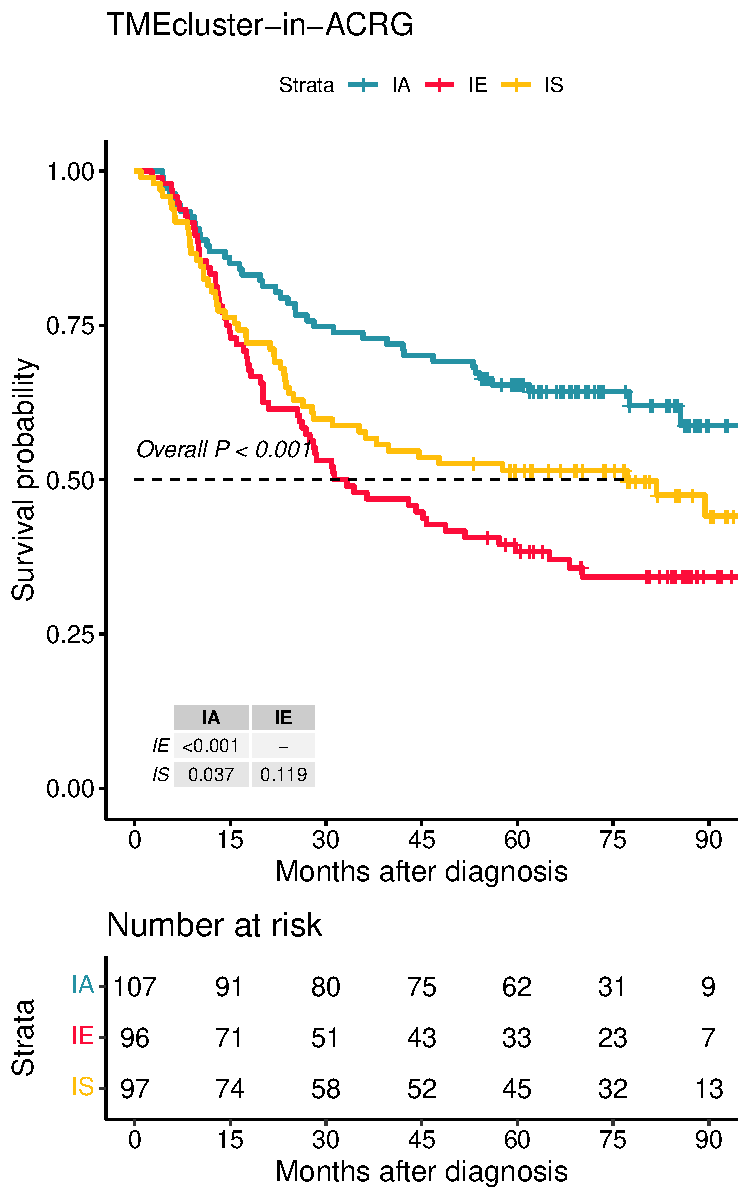
\includegraphics{tme-deg-gsea_files/figure-latex/unnamed-chunk-20-1.pdf}

\begin{Shaded}
\begin{Highlighting}[]
\NormalTok{p1}\OtherTok{\textless{}{-}} \FunctionTok{percent\_bar\_plot}\NormalTok{(input, }\AttributeTok{x =} \StringTok{"TMEcluster"}\NormalTok{ , }\AttributeTok{y =} \StringTok{"Subtype"}\NormalTok{, }\AttributeTok{palette =} \StringTok{"jama"}\NormalTok{)}
\end{Highlighting}
\end{Shaded}

\begin{verbatim}
## # A tibble: 12 x 5
## # Groups:   TMEcluster [3]
##    TMEcluster Subtype    Freq  Prop count
##    <chr>      <fct>     <dbl> <dbl> <dbl>
##  1 IA         EMT           7  0.07   107
##  2 IA         MSI          49  0.46   107
##  3 IA         MSS/TP53-    27  0.25   107
##  4 IA         MSS/TP53+    24  0.22   107
##  5 IE         EMT          24  0.25    96
##  6 IE         MSI           3  0.03    96
##  7 IE         MSS/TP53-    40  0.42    96
##  8 IE         MSS/TP53+    29  0.3     96
##  9 IS         EMT          15  0.15    97
## 10 IS         MSI          16  0.16    97
## 11 IS         MSS/TP53-    40  0.41    97
## 12 IS         MSS/TP53+    26  0.27    97
## [1] "'#374E55FF', '#DF8F44FF', '#00A1D5FF', '#B24745FF', '#79AF97FF', '#6A6599FF', '#80796BFF'"
\end{verbatim}

\begin{Shaded}
\begin{Highlighting}[]
\NormalTok{p2}\OtherTok{\textless{}{-}} \FunctionTok{percent\_bar\_plot}\NormalTok{(input, }\AttributeTok{x =} \StringTok{"TMEcluster"}\NormalTok{ , }\AttributeTok{y =} \StringTok{"Lauren"}\NormalTok{, }\AttributeTok{palette =} \StringTok{"jama"}\NormalTok{)}
\end{Highlighting}
\end{Shaded}

\begin{verbatim}
## # A tibble: 9 x 5
## # Groups:   TMEcluster [3]
##   TMEcluster Lauren      Freq  Prop count
##   <chr>      <fct>      <dbl> <dbl> <dbl>
## 1 IA         Diffuse       34  0.32   107
## 2 IA         Intestinal    60  0.56   107
## 3 IA         Mixed         13  0.12   107
## 4 IE         Diffuse       60  0.62    96
## 5 IE         Intestinal    32  0.33    96
## 6 IE         Mixed          4  0.04    96
## 7 IS         Diffuse       41  0.42    97
## 8 IS         Intestinal    54  0.56    97
## 9 IS         Mixed          2  0.02    97
## [1] "'#374E55FF', '#DF8F44FF', '#00A1D5FF', '#B24745FF', '#79AF97FF', '#6A6599FF', '#80796BFF'"
\end{verbatim}

\begin{Shaded}
\begin{Highlighting}[]
\NormalTok{p3}\OtherTok{\textless{}{-}} \FunctionTok{percent\_bar\_plot}\NormalTok{(input, }\AttributeTok{x =} \StringTok{"TMEcluster"}\NormalTok{ , }\AttributeTok{y =} \StringTok{"TMEscore\_binary"}\NormalTok{, }\AttributeTok{palette =} \StringTok{"jama"}\NormalTok{)}
\end{Highlighting}
\end{Shaded}

\begin{verbatim}
## # A tibble: 7 x 5
## # Groups:   TMEcluster [3]
##   TMEcluster TMEscore_binary  Freq  Prop count
##   <chr>      <fct>           <dbl> <dbl> <dbl>
## 1 IA         High               60  0.56   107
## 2 IA         Low                47  0.44   107
## 3 IE         High                5  0.05    96
## 4 IE         Low                91  0.95    96
## 5 IS         High                6  0.06    97
## 6 IS         Low                90  0.93    97
## 7 IS         <NA>                1  0.01    97
## [1] "'#374E55FF', '#DF8F44FF', '#00A1D5FF', '#B24745FF', '#79AF97FF', '#6A6599FF', '#80796BFF'"
\end{verbatim}

\begin{Shaded}
\begin{Highlighting}[]
\NormalTok{p1}\SpecialCharTok{|}\NormalTok{p2}\SpecialCharTok{|}\NormalTok{p3}
\end{Highlighting}
\end{Shaded}

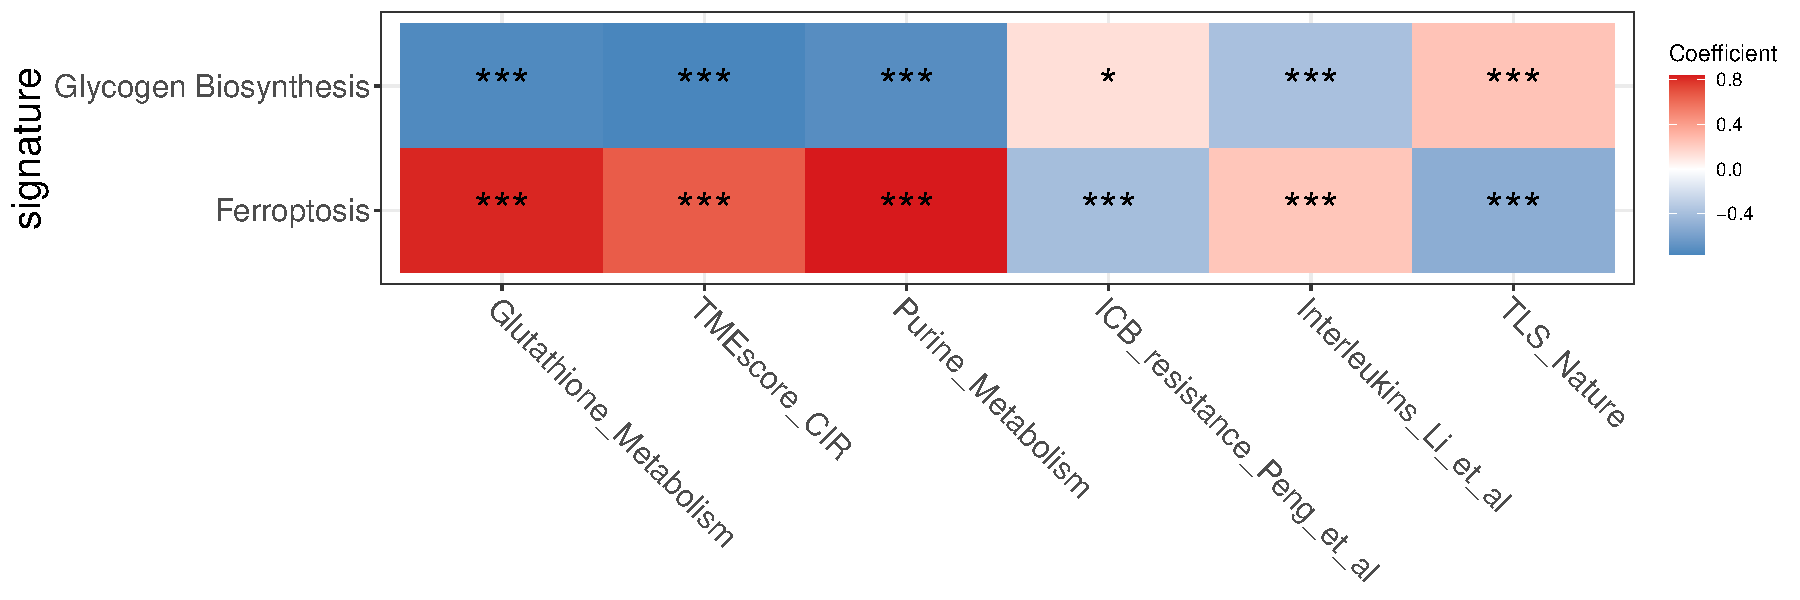
\includegraphics{tme-deg-gsea_files/figure-latex/unnamed-chunk-22-1.pdf}

\hypertarget{references-4}{%
\section{References}\label{references-4}}

Cristescu, R., Lee, J., Nebozhyn, M. et al.~Molecular analysis of gastric cancer identifies subtypes associated with distinct clinical outcomes. Nat Med 21, 449--456 (2015). \url{https://doi.org/10.1038/nm.3850}

\href{https://cibersort.stanford.edu/}{CIBERSORT}; Newman, A. M., Liu, C. L., Green, M. R., Gentles, A. J., Feng, W., Xu, Y., \ldots{} Alizadeh, A. A. (2015). Robust enumeration of cell subsets from tissue expression profiles. Nature Methods, 12(5), 453--457. \url{https://doi.org/10.1038/nmeth.3337};

Seurat: Hao and Hao et al.~Integrated analysis of multimodal single-cell data. Cell (2021)

Zeng D, Yu Y, Qiu W, Mao Q, \ldots, Zhang K, Liao W; Tumor microenvironment immunotyping heterogeneity reveals distinct molecular mechanisms to clinical immunotherapy applications in gastric cancer. (2023) Under Review.

\hypertarget{tme-and-genomic-interaction}{%
\chapter{\texorpdfstring{\textbf{TME and genomic interaction}}{TME and genomic interaction}}\label{tme-and-genomic-interaction}}

\hypertarget{loading-packages-6}{%
\section{Loading packages}\label{loading-packages-6}}

\begin{Shaded}
\begin{Highlighting}[]
\FunctionTok{library}\NormalTok{(IOBR)}
\end{Highlighting}
\end{Shaded}

\hypertarget{genomic-data-prepare}{%
\section{Genomic data prepare}\label{genomic-data-prepare}}

MAF data was download from \href{https://xenabrowser.net/datapages/}{UCSC Xena hub}
In this example, we used the maf file of TCGA-STAD to extract the SNPs in it,and then transformed it into a non-negative matrix.

\begin{Shaded}
\begin{Highlighting}[]
\NormalTok{maf\_file }\OtherTok{\textless{}{-}}\StringTok{"./TCGA.STAD.mutect.c06465a3{-}50e7{-}46f7{-}b2dd{-}7bd654ca206b.DR{-}10.0.somatic.maf"}
\NormalTok{mut\_list }\OtherTok{\textless{}{-}} \FunctionTok{make\_mut\_matrix}\NormalTok{(}\AttributeTok{maf =}\NormalTok{ maf\_file, }\AttributeTok{isTCGA   =}\NormalTok{ T, }\AttributeTok{category =} \StringTok{"multi"}\NormalTok{)}
\end{Highlighting}
\end{Shaded}

\begin{verbatim}
## -Reading
## -Validating
## -Silent variants: 70967 
## -Summarizing
## --Possible FLAGS among top ten genes:
##   TTN
##   MUC16
##   SYNE1
##   FLG
## -Processing clinical data
## --Missing clinical data
## -Finished in 15.0s elapsed (14.7s cpu) 
##        Frame_Shift_Del        Frame_Shift_Ins           In_Frame_Del 
##                  18418                   4461                    692 
##           In_Frame_Ins      Missense_Mutation      Nonsense_Mutation 
##                    268                 109669                   6011 
##       Nonstop_Mutation            Splice_Site Translation_Start_Site 
##                    107                   2445                    106 
##    DEL    INS    SNP 
##  19387   4900 117890
\end{verbatim}

\begin{Shaded}
\begin{Highlighting}[]
\NormalTok{mut }\OtherTok{\textless{}{-}}\NormalTok{ mut\_list}\SpecialCharTok{$}\NormalTok{snp}
\end{Highlighting}
\end{Shaded}

\hypertarget{identifying-mutations-associated-with-tme}{%
\section{Identifying Mutations Associated with TME}\label{identifying-mutations-associated-with-tme}}

The microenvironmental data from the TCGA-STAD expression matrix was merged. The Cuzick or Wilcoxon test was used to identify genetic variants associated with microenvironmental factors. CD\_8\_T\_effector was used as the target variable in this example.

\begin{Shaded}
\begin{Highlighting}[]
\FunctionTok{data}\NormalTok{(}\StringTok{"tcga\_stad\_sig"}\NormalTok{, }\AttributeTok{package =} \StringTok{"IOBR"}\NormalTok{)}
\NormalTok{res}\OtherTok{\textless{}{-}}\FunctionTok{find\_mutations}\NormalTok{(}\AttributeTok{mutation\_matrix     =}\NormalTok{ mut, }
                    \AttributeTok{signature\_matrix    =}\NormalTok{ tcga\_stad\_sig, }
                    \AttributeTok{id\_signature\_matrix =} \StringTok{"ID"}\NormalTok{, }
                    \AttributeTok{signature           =} \StringTok{"CD\_8\_T\_effector"}\NormalTok{,}
                    \AttributeTok{min\_mut\_freq        =} \FloatTok{0.01}\NormalTok{, }
                    \AttributeTok{plot                =} \ConstantTok{TRUE}\NormalTok{, }
                    \AttributeTok{jitter              =} \ConstantTok{TRUE}\NormalTok{, }
                    \AttributeTok{point.alpha         =} \FloatTok{0.25}\NormalTok{)}
\end{Highlighting}
\end{Shaded}

\begin{verbatim}
## [1] ">>>> Result of Cuzick Test"
##             p.value  names statistic adjust_pvalue
## PIK3CA 3.148160e-09 PIK3CA  5.923680  1.574080e-06
## SPEG   9.070928e-05   SPEG  3.914187  2.267732e-02
## TCHH   4.409469e-04   TCHH  3.514281  5.740100e-02
## PLXNA4 5.420662e-04 PLXNA4  3.459059  5.740100e-02
## ARID1A 5.805905e-04 ARID1A  3.440523  5.740100e-02
## WDFY3  6.888120e-04  WDFY3  3.393994  5.740100e-02
## GTF3C1 8.120095e-04 GTF3C1  3.348668  5.800068e-02
## DMD    1.675467e-03    DMD  3.142439  6.972915e-02
## CR1    1.775997e-03    CR1  3.125340  6.972915e-02
## EP300  2.042083e-03  EP300  3.084043  6.972915e-02
\end{verbatim}

\begin{verbatim}
## [1] ">>> Result of Wilcoxon test (top 10)"
##             p.value  names statistic adjust_pvalue
## PIK3CA 1.921035e-10 PIK3CA      4125  9.605174e-08
## TCHH   1.961642e-05   TCHH      3312  4.904106e-03
## SPEG   3.532750e-05   SPEG      1947  5.887916e-03
## LRP1   7.511741e-05   LRP1      2649  9.389676e-03
## WDFY3  1.257659e-04  WDFY3      2964  1.257659e-02
## ARID1A 2.468609e-04 ARID1A      4878  2.057174e-02
## PLXNA4 4.215809e-04 PLXNA4      3638  3.011292e-02
## ANK3   6.399572e-04   ANK3      4446  3.933979e-02
## DMD    7.364591e-04    DMD      5311  3.933979e-02
## PLEC   8.026240e-04   PLEC      5562  3.933979e-02
\end{verbatim}

\begin{verbatim}
## All mutation types: mut.
\end{verbatim}

\begin{verbatim}
## Warning: You defined `cell_fun` for a heatmap with more than 100 rows or
## columns, which might be very slow to draw. Consider to use the
## vectorized version `layer_fun`.
\end{verbatim}

\begin{verbatim}
## All mutation types: mut.
\end{verbatim}

\begin{verbatim}
## Warning: You defined `cell_fun` for a heatmap with more than 100 rows or
## columns, which might be very slow to draw. Consider to use the
## vectorized version `layer_fun`.
\end{verbatim}

\hypertarget{oncoprint-of-result}{%
\section{OncoPrint of result}\label{oncoprint-of-result}}

\begin{figure}

{\centering 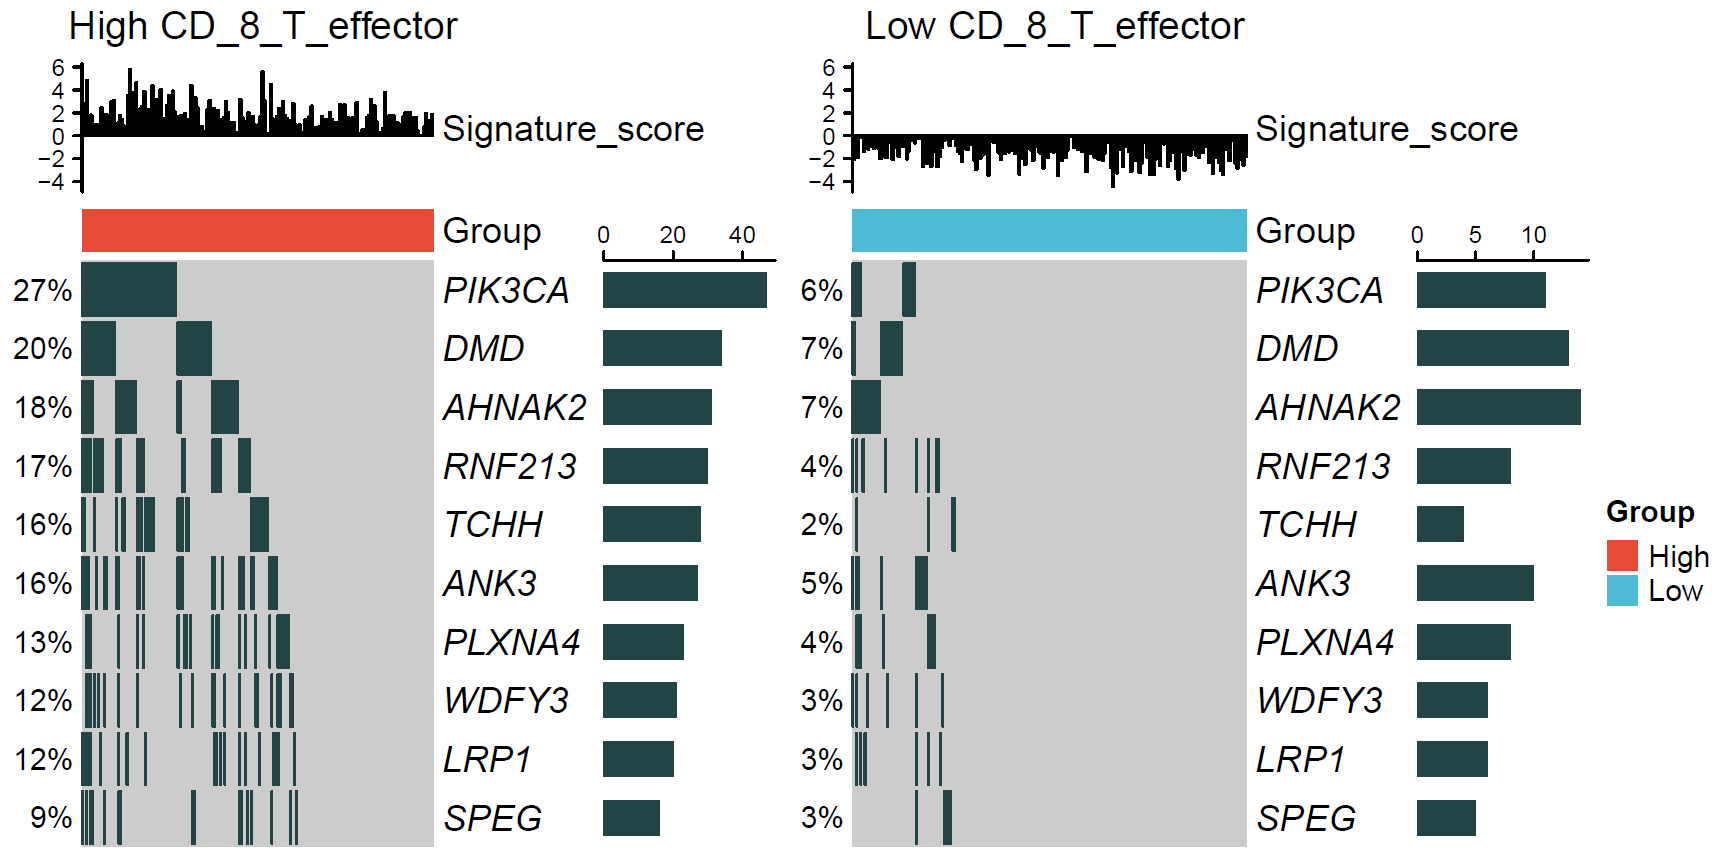
\includegraphics[width=0.95\linewidth]{./fig/0-OncoPrint-CD_8_T_effector} 

}

\caption{OncoPrint}\label{fig:unnamed-chunk-4}
\end{figure}

\hypertarget{boxplot-of-top-10-mutated-genes}{%
\section{Boxplot of top 10 mutated genes}\label{boxplot-of-top-10-mutated-genes}}

\begin{figure}

{\centering 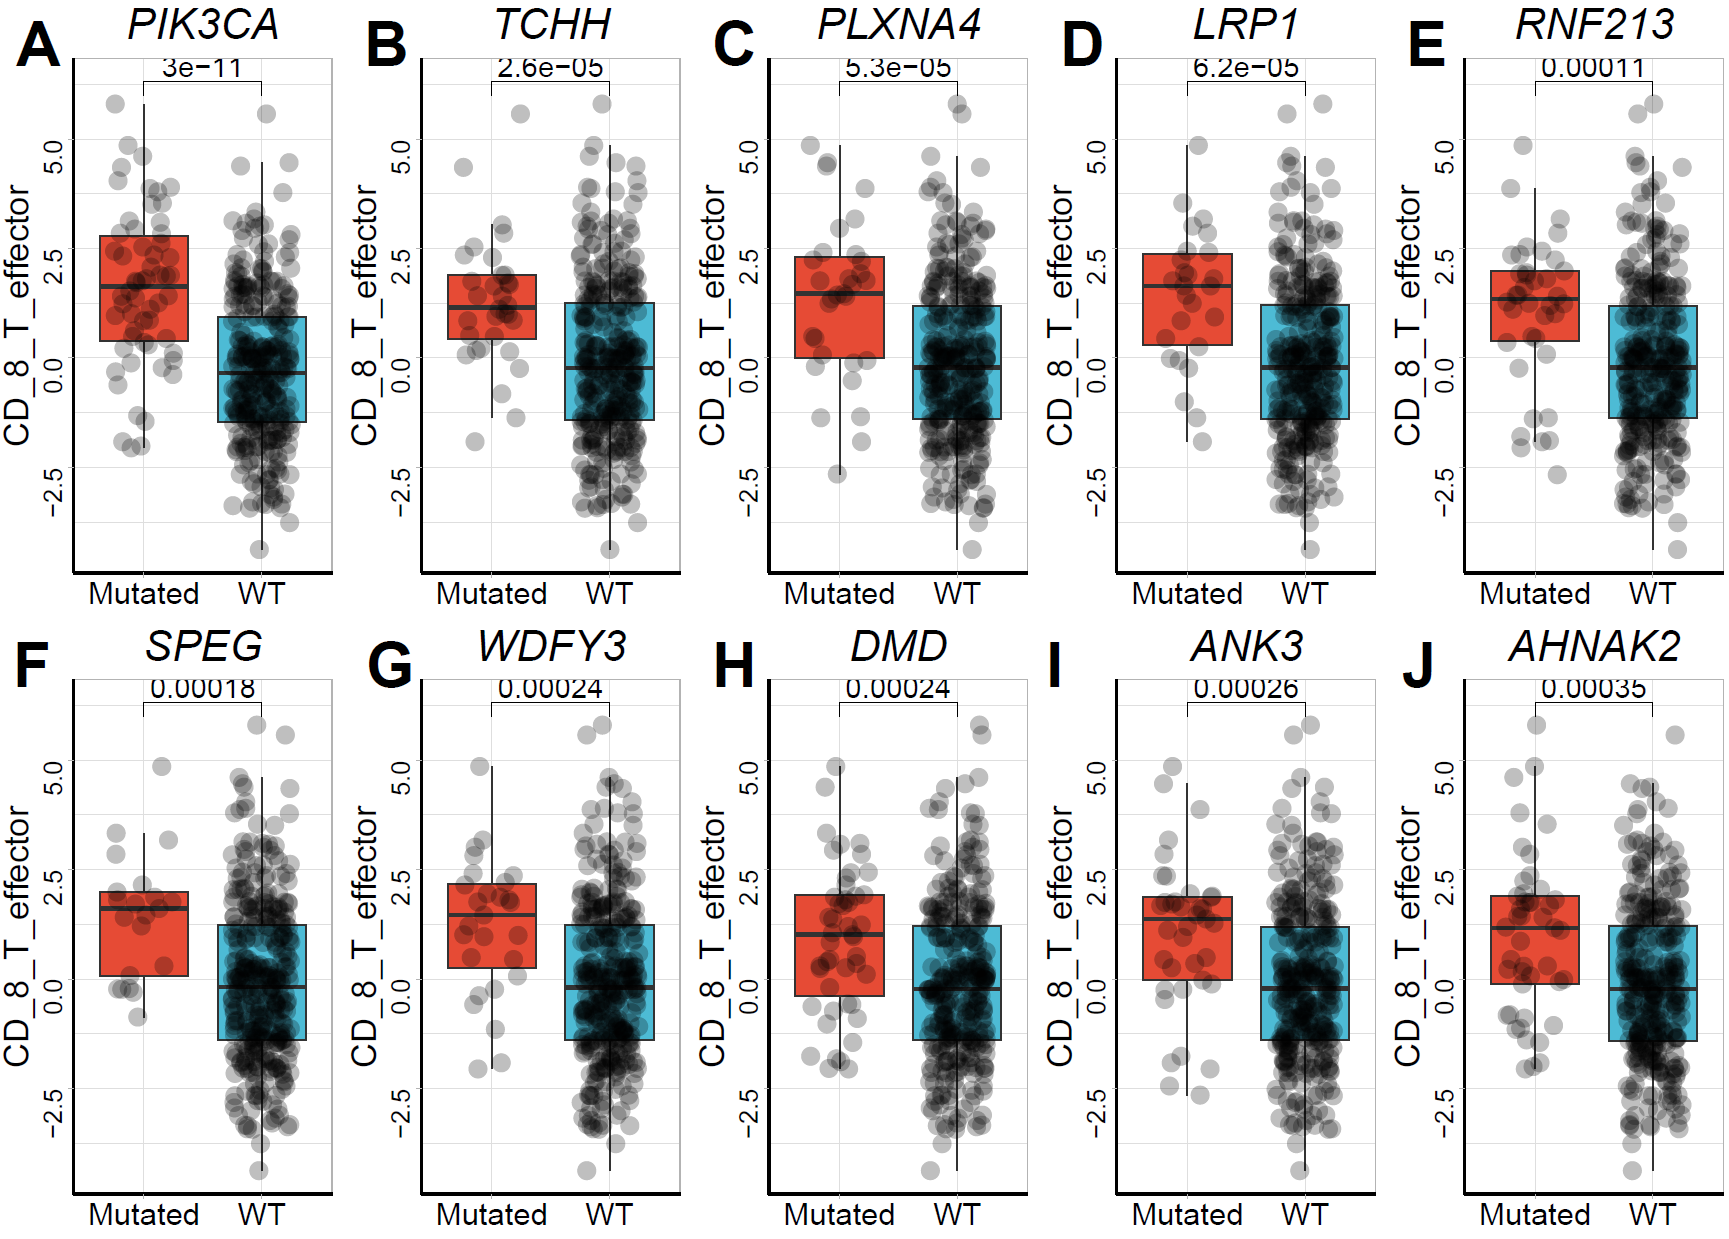
\includegraphics[width=0.95\linewidth]{./fig/4-Relevant_mutations_binary} 

}

\caption{Top 10 mutated genes}\label{fig:unnamed-chunk-5}
\end{figure}

\hypertarget{references-5}{%
\section{References}\label{references-5}}

Gu, Z. (2022) Complex Heatmap Visualization. iMeta.

Anand Mayakonda et al., (2018) Maftools: efficient and comprehensive analysis of somatic variants in cancer. Genome Research

\hypertarget{tme-modeling}{%
\chapter{\texorpdfstring{\textbf{TME Modeling}}{TME Modeling}}\label{tme-modeling}}

Previous studies have shown that the tumour microenvironment is a complex ecosystem. No single cell or gene is sufficient to influence the phenotype. Therefore, machine learning models of the tumour microenvironment or models of tumour microenvironment typing are used to predict tumour phenotypes and treatment response. In the last section, we present common considerations and scenarios for constructing tumour microenvironment models.

\hypertarget{loading-packages-7}{%
\section{Loading packages}\label{loading-packages-7}}

\begin{Shaded}
\begin{Highlighting}[]
\FunctionTok{library}\NormalTok{(IOBR)}
\end{Highlighting}
\end{Shaded}

\hypertarget{data-prepare}{%
\section{Data prepare}\label{data-prepare}}

Using data from IMvigor210, we demonstrate two common scenarios for building models of the tumour microenvironment: predicting survival and predicting treatment response (BOR, RECIEST 1.1).

\begin{Shaded}
\begin{Highlighting}[]
\FunctionTok{data}\NormalTok{(}\StringTok{"imvigor210\_sig"}\NormalTok{, }\AttributeTok{package =} \StringTok{"IOBR"}\NormalTok{)}
\FunctionTok{data}\NormalTok{(}\StringTok{"imvigor210\_pdata"}\NormalTok{, }\AttributeTok{package =} \StringTok{"IOBR"}\NormalTok{)}
\end{Highlighting}
\end{Shaded}

\hypertarget{input-data-overall-survival-prepare}{%
\section{Input data (overall survival) prepare}\label{input-data-overall-survival-prepare}}

\begin{Shaded}
\begin{Highlighting}[]
\NormalTok{pdata\_prog }\OtherTok{\textless{}{-}}\NormalTok{ imvigor210\_pdata }\SpecialCharTok{\%\textgreater{}\%} 
\NormalTok{  dplyr}\SpecialCharTok{::}\FunctionTok{select}\NormalTok{(ID, OS\_days, OS\_status) }\SpecialCharTok{\%\textgreater{}\%}
  \FunctionTok{mutate}\NormalTok{(}\AttributeTok{OS\_days =} \FunctionTok{as.numeric}\NormalTok{(.}\SpecialCharTok{$}\NormalTok{OS\_days)) }\SpecialCharTok{\%\textgreater{}\%} 
  \FunctionTok{mutate}\NormalTok{(}\AttributeTok{OS\_status =} \FunctionTok{as.numeric}\NormalTok{(.}\SpecialCharTok{$}\NormalTok{OS\_status))}

\FunctionTok{head}\NormalTok{(pdata\_prog)}
\end{Highlighting}
\end{Shaded}

\begin{verbatim}
## # A tibble: 6 x 3
##   ID              OS_days OS_status
##   <chr>             <dbl>     <dbl>
## 1 SAM00b9e5c52da9    57.2         1
## 2 SAM0257bbbbd388   469.          1
## 3 SAM025b45c27e05   263.          1
## 4 SAM032c642382a7    74.9         1
## 5 SAM04c589eb3fb3    20.7         0
## 6 SAM0571f17f4045   136.          1
\end{verbatim}

\hypertarget{constructing-survival-prediction-models}{%
\section{Constructing survival prediction models}\label{constructing-survival-prediction-models}}

\begin{Shaded}
\begin{Highlighting}[]
\NormalTok{prognostic\_result }\OtherTok{\textless{}{-}} \FunctionTok{PrognosticModel}\NormalTok{(}\AttributeTok{x           =}\NormalTok{ imvigor210\_sig, }
                                     \AttributeTok{y           =}\NormalTok{ pdata\_prog, }
                                     \AttributeTok{scale       =}\NormalTok{ T, }
                                     \AttributeTok{seed        =} \DecValTok{123456}\NormalTok{, }
                                     \AttributeTok{train\_ratio =} \FloatTok{0.7}\NormalTok{, }
                                     \AttributeTok{nfold       =} \DecValTok{8}\NormalTok{,}
                                     \AttributeTok{plot        =} \ConstantTok{TRUE}\NormalTok{)}
\end{Highlighting}
\end{Shaded}

\begin{verbatim}
## NULL
## NULL
## NULL
\end{verbatim}

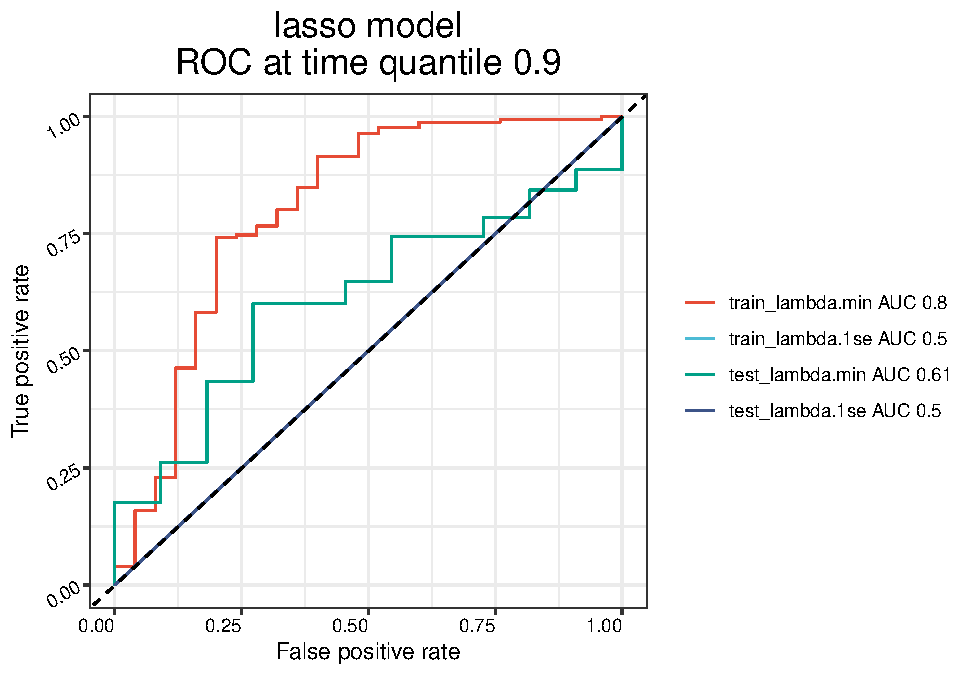
\includegraphics{tme-modeling_files/figure-latex/unnamed-chunk-4-1.pdf} 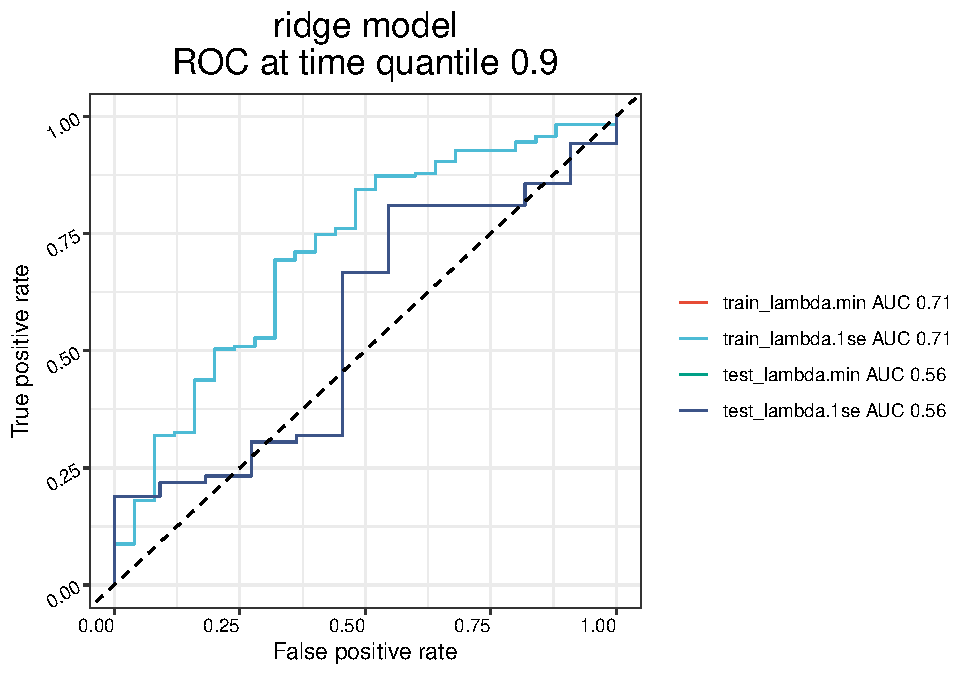
\includegraphics{tme-modeling_files/figure-latex/unnamed-chunk-4-2.pdf}

\hypertarget{input-data-response-prepare}{%
\section{Input data (Response) prepare}\label{input-data-response-prepare}}

\begin{Shaded}
\begin{Highlighting}[]
\NormalTok{pdata\_group }\OtherTok{\textless{}{-}}\NormalTok{ imvigor210\_pdata[}\SpecialCharTok{!}\NormalTok{imvigor210\_pdata}\SpecialCharTok{$}\NormalTok{BOR\_binary}\SpecialCharTok{==}\StringTok{"NA"}\NormalTok{,}\FunctionTok{c}\NormalTok{(}\StringTok{"ID"}\NormalTok{,}\StringTok{"BOR\_binary"}\NormalTok{)]}
\NormalTok{pdata\_group}\SpecialCharTok{$}\NormalTok{BOR\_binary }\OtherTok{\textless{}{-}} \FunctionTok{ifelse}\NormalTok{(pdata\_group}\SpecialCharTok{$}\NormalTok{BOR\_binary }\SpecialCharTok{==} \StringTok{"R"}\NormalTok{, }\DecValTok{1}\NormalTok{, }\DecValTok{0}\NormalTok{)}
\FunctionTok{head}\NormalTok{(pdata\_group)}
\end{Highlighting}
\end{Shaded}

\begin{verbatim}
## # A tibble: 6 x 2
##   ID              BOR_binary
##   <chr>                <dbl>
## 1 SAM0257bbbbd388          0
## 2 SAM025b45c27e05          0
## 3 SAM032c642382a7          0
## 4 SAM0571f17f4045          0
## 5 SAM065890737112          1
## 6 SAM0684af734db1          1
\end{verbatim}

\hypertarget{constructing-prediction-models-for-response}{%
\section{Constructing prediction models for response}\label{constructing-prediction-models-for-response}}

\begin{Shaded}
\begin{Highlighting}[]
\NormalTok{binom\_res }\OtherTok{\textless{}{-}} \FunctionTok{BinomialModel}\NormalTok{(}\AttributeTok{x           =}\NormalTok{ imvigor210\_sig, }
                           \AttributeTok{y           =}\NormalTok{ pdata\_group, }
                           \AttributeTok{seed        =} \DecValTok{123456}\NormalTok{, }
                           \AttributeTok{scale       =} \ConstantTok{TRUE}\NormalTok{, }
                           \AttributeTok{train\_ratio =} \FloatTok{0.7}\NormalTok{, }
                           \AttributeTok{nfold       =} \DecValTok{8}\NormalTok{, }
                           \AttributeTok{plot        =}\NormalTok{ T)}
\end{Highlighting}
\end{Shaded}

\begin{verbatim}
## NULL
## NULL
## NULL
\end{verbatim}

\begin{verbatim}
## NULL
\end{verbatim}

\includegraphics{tme-modeling_files/figure-latex/unnamed-chunk-6-1.pdf} 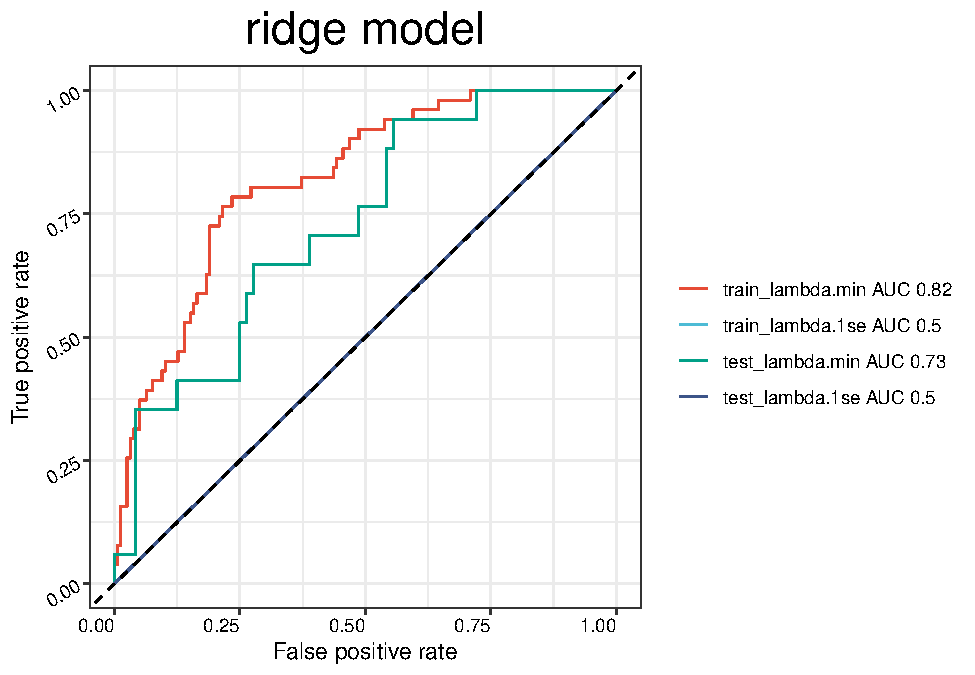
\includegraphics{tme-modeling_files/figure-latex/unnamed-chunk-6-2.pdf}

\begin{verbatim}
## NULL
\end{verbatim}

\hypertarget{references-6}{%
\section{References}\label{references-6}}

Cristescu, R., Lee, J., Nebozhyn, M. et al.~Molecular analysis of gastric cancer identifies subtypes associated with distinct clinical outcomes. Nat Med 21, 449--456 (2015). \url{https://doi.org/10.1038/nm.3850}

\href{https://cibersort.stanford.edu/}{CIBERSORT}; Newman, A. M., Liu, C. L., Green, M. R., Gentles, A. J., Feng, W., Xu, Y., \ldots{} Alizadeh, A. A. (2015). Robust enumeration of cell subsets from tissue expression profiles. Nature Methods, 12(5), 453--457. \url{https://doi.org/10.1038/nmeth.3337};

Seurat: Hao and Hao et al.~Integrated analysis of multimodal single-cell data. Cell (2021)

\hypertarget{references-7}{%
\chapter{\texorpdfstring{\textbf{References}}{References}}\label{references-7}}

If IOBR R package is utilized in your published research, please cite:

Zeng D, Ye Z, Shen R, Yu G, Wu J, Xiong Y,\ldots, Liao W (2021) \textbf{IOBR}: Multi-Omics Immuno-Oncology Biological Research to Decode Tumor Microenvironment and Signatures. \emph{Frontiers in Immunology}. 12:687975. \href{https://www.frontiersin.org/articles/10.3389/fimmu.2021.687975/full}{doi: 10.3389/fimmu.2021.687975}

\hypertarget{tme-deconvolution-1}{%
\section{TME deconvolution}\label{tme-deconvolution-1}}

Please cite the following papers appropriately for TME deconvolution algorithm if used:

\textbf{CIBERSORT}: Newman, A. M., Liu, C. L., Green, M. R., Gentles, A. J., Feng, W., Xu, Y., \ldots{} Alizadeh, A. A. (2015). Robust enumeration of cell subsets from tissue expression profiles. Nature Methods, 12(5), 453--457. \url{https://doi.org/10.1038/nmeth.3337}

\textbf{ESTIMATE}: Vegesna R, Kim H, Torres-Garcia W, \ldots, Verhaak R.*(2013). Inferring tumour purity and stromal and immune cell admixture from expression data. Nature Communications 4, 2612. \url{http://doi.org/10.1038/ncomms3612}

\textbf{quanTIseq}: Finotello, F., Mayer, C., Plattner, C., Laschober, G., Rieder, D., Hackl, H., \ldots, Sopper, S.* (2019). Molecular and pharmacological modulators of the tumor immune contexture revealed by deconvolution of RNA-seq data. Genome medicine, 11(1), 34. \url{https://doi.org/10.1186/s13073-019-0638-6}

\textbf{TIMER}: Li, B., Severson, E., Pignon, J.-C., Zhao, H., Li, T., Novak, J., \ldots{} Liu, X. S.* (2016). Comprehensive analyses of tumor immunity: implications for cancer immunotherapy. Genome Biology, 17(1), 174.

\textbf{IPS}: P. Charoentong et al.*, Pan-cancer Immunogenomic Analyses Reveal Genotype-Immunophenotype Relationships and Predictors of Response to Checkpoint Blockade. Cell Reports 18, 248-262 (2017). \url{https://doi.org/10.1016/j.celrep.2016.12.019}

\textbf{MCPCounter}: Becht, E., Giraldo, N. A., Lacroix, L., Buttard, B., Elarouci, N., Petitprez, F., \ldots{} de Reyniès, A*. (2016). Estimating the population abundance of tissue-infiltrating immune and stromal cell populations using gene expression. Genome Biology, 17(1), 218. \url{https://doi.org/10.1186/s13059-016-1070-5}

\textbf{xCell}: Aran, D., Hu, Z., \& Butte, A. J.* (2017). xCell: digitally portraying the tissue cellular heterogeneity landscape. Genome Biology, 18(1), 220. \url{https://doi.org/10.1186/s13059-017-1349-1}

\textbf{EPIC}: Racle, J., de Jonge, K., Baumgaertner, P., Speiser, D. E., \& Gfeller, D*. (2017). Simultaneous enumeration of cancer and immune cell types from bulk tumor gene expression data. ELife, 6, e26476. \url{https://doi.org/10.7554/eLife.26476}

\hypertarget{tme-signatures}{%
\section{TME Signatures}\label{tme-signatures}}

For signature score estimation, please cite corresponding literature below:

\textbf{ssgsea}: Barbie, D.A. et al (2009). Systematic RNA interference reveals that oncogenic KRAS-driven cancers require TBK1. Nature, 462(5):108-112.

\textbf{gsva}: Hänzelmann, S., Castelo, R. and Guinney, J. (2013). GSVA: Gene set variation analysis for microarray and RNA-Seq data. BMC Bioinformatics, 14(1):7.

\textbf{zscore}: Lee, E. et al (2008). Inferring pathway activity toward precise disease classification. PLoS Comp Biol, 4(11):e1000217.

\hypertarget{data-sets}{%
\section{Data sets}\label{data-sets}}

For the datasets enrolled in IOBR, please cite the data sources:

\textbf{UCSCXena}: Wang et al.,et al (2019). The UCSCXenaTools R package: a toolkit for accessing genomics data from UCSC Xena platform, from cancer multi-omics to single-cell RNA-seq. Journal of Open Source Software, 4(40), 1627

\textbf{TLSscore}: Helmink BA, Reddy SM, Gao J, et al.~B cells and tertiary lymphoid structures promote immunotherapy response. Nature. 2020 Jan;577(7791):549-555.

\textbf{IMvigor210 immuntherapy cohort}: Mariathasan S, Turley SJ, Nickles D, et al.~TGFβ attenuates tumour response to PD-L1 blockade by contributing to exclusion of T cells. Nature. 2018 Feb 22;554(7693):544-548.
\textbf{HCP5}: Kulski, J.K. Long Noncoding RNA HCP5, a Hybrid HLA Class I Endogenous Retroviral Gene: Structure, Expression, and Disease Associations. Cells 2019, 8, 480.

\textbf{HCP5}: Li, Y., Jiang, T., Zhou, W. et al.~Pan-cancer characterization of immune-related lncRNAs identifies potential oncogenic biomarkers. Nat Commun 11, 1000 (2020).
HCP5: Sun J, Zhang Z, Bao S, et alIdentification of tumor immune infiltration-associated lncRNAs for improving prognosis and immunotherapy response of patients with non-small cell lung cancerJournal for ImmunoTherapy of Cancer 2020;8:e000110.

\textbf{LINC00657}: Feng Q, Zhang H, Yao D, Chen WD, Wang YD. Emerging Role of Non-Coding RNAs in Esophageal Squamous Cell Carcinoma. Int J Mol Sci. 2019 Dec 30;21(1):258. doi: 10.3390/ijms21010258.

\textbf{LINC00657}: Qin X, Zhou M, Lv H, Mao X, Li X, Guo H, Li L, Xing H. Long noncoding RNA LINC00657 inhibits cervical cancer development by sponging miR-20a-5p and targeting RUNX3. Cancer Lett. 2020 Oct 28:S0304-3835(20)30578-4. doi: 10.1016/j.canlet.2020.10.044.
\textbf{LINC00657}: Zhang XM, Wang J, Liu ZL, Liu H, Cheng YF, Wang T. LINC00657/miR-26a-5p/CKS2 ceRNA network promotes the growth of esophageal cancer cells via the MDM2/p53/Bcl2/Bax pathway. Biosci Rep.~2020;40(6):BSR20200525.

\textbf{TCGA-STAD}: Cancer Genome Atlas Research Network. Comprehensive molecular characterization of gastric adenocarcinoma. Nature. 2014 Sep 11;513(7517):202-9. doi: 10.1038/nature13480.
TCGA.STAD MAF data: \url{https://api.gdc.cancer.gov/data/c06465a3-50e7-46f7-b2dd-7bd654ca206b}

\hypertarget{others}{%
\section{Others}\label{others}}

\begin{enumerate}
\def\labelenumi{\arabic{enumi}.}
\item
  Newman, A. M., Liu, C. L., Green, M. R., Gentles, A. J., Feng, W., Xu, Y., \ldots{} Alizadeh, A. A. (2015). Robust enumeration of cell subsets from tissue expression profiles. Nature Methods, 12(5), 453--457.
\item
  Vegesna R, Kim H, Torres-Garcia W, \ldots, Verhaak R.*(2013). Inferring tumour purity and stromal and immune cell admixture from expression data. Nature Communications 4, 2612.
\item
  Rieder, D., Hackl, H., \ldots, Sopper, S.* (2019). Molecular and pharmacological modulators of the tumor immune contexture revealed by deconvolution of RNA-seq data. Genome medicine, 11(1), 34.
\item
  Li, B., Severson, E., Pignon, J.-C., Zhao, H., Li, T., Novak, J., \ldots{} Liu, X. S.* (2016). Comprehensive analyses of tumor immunity: implications for cancer immunotherapy. Genome Biology, 17(1), 174.
\item
  P. Charoentong et al.*, Pan-cancer Immunogenomic Analyses Reveal Genotype-Immunophenotype Relationships and Predictors of Response to Checkpoint Blockade. Cell Reports 18, 248-262 (2017).
\item
  Becht, E., Giraldo, N. A., Lacroix, L., Buttard, B., Elarouci, N., Petitprez, F., \ldots{} de Reyniès, A*. (2016). Estimating the population abundance of tissue-infiltrating immune and stromal cell populations using gene expression. Genome Biology, 17(1), 218.
\item
  Aran, D., Hu, Z., \& Butte, A. J.* (2017). xCell: digitally portraying the tissue cellular heterogeneity landscape. Genome Biology, 18(1), 220.
\item
  Racle, J., de Jonge, K., Baumgaertner, P., Speiser, D. E., \& Gfeller, D*. (2017). Simultaneous enumeration of cancer and immune cell types from bulk tumor gene expression data. ELife, 6, e26476.
\item
  Barbie, D.A. et al (2009). Systematic RNA interference reveals that oncogenic KRAS-driven cancers require TBK1. Nature, 462(5):108-112.
\item
  Hänzelmann, S., Castelo, R. and Guinney, J. (2013). GSVA: Gene set variation analysis for microarray and RNA-Seq data. BMC Bioinformatics, 14(1):7.
\item
  Lee, E. et al (2008). Inferring pathway activity toward precise disease classification. PLoS Comp Biol, 4(11):e1000217.
\item
  Wang et al.,et al (2019). The UCSCXenaTools R package: a toolkit for accessing genomics data from UCSC Xena platform, from cancer multi-omics to single-cell RNA-seq. Journal of Open Source Software, 4(40), 1627
\item
  Helmink BA, Reddy SM, Gao J, et al.~B cells and tertiary lymphoid structures promote immunotherapy response. Nature. 2020 Jan;577(7791):549-555.
\item
  Mariathasan S, Turley SJ, Nickles D, et al.~TGFβ attenuates tumour response to PD-L1 blockade by contributing to exclusion of T cells. Nature. 2018 Feb 22;554(7693):544-548.
\item
  Kulski, J.K. Long Noncoding RNA HCP5, a Hybrid HLA Class I Endogenous Retroviral Gene: Structure, Expression, and Disease Associations. Cells 2019, 8, 480.
\item
  Li, Y., Jiang, T., Zhou, W. et al.~Pan-cancer characterization of immune-related lncRNAs identifies potential oncogenic biomarkers. Nat Commun 11, 1000 (2020).
\item
  Sun J, Zhang Z, Bao S, et alIdentification of tumor immune infiltration-associated lncRNAs for improving prognosis and immunotherapy response of patients with non-small cell lung cancerJournal for ImmunoTherapy of Cancer 2020;8:e000110.
\item
  Feng Q, Zhang H, Yao D, Chen WD, Wang YD. Emerging Role of Non-Coding RNAs in Esophageal Squamous Cell Carcinoma. Int J Mol Sci. 2019 Dec 30;21(1):258. doi: 10.3390/ijms21010258.
\item
  Qin X, Zhou M, Lv H, Mao X, Li X, Guo H, Li L, Xing H. Long noncoding RNA LINC00657 inhibits cervical cancer development by sponging miR-20a-5p and targeting RUNX3. Cancer Lett. 2020 Oct
\item
  Zhang XM, Wang J, Liu ZL, Liu H, Cheng YF, Wang T. LINC00657/miR-26a-5p/CKS2 ceRNA network promotes the growth of esophageal cancer cells via the MDM2/p53/Bcl2/Bax pathway. Biosci Rep.~2020;40(6):BSR20200525.
\item
  Cancer Genome Atlas Research Network. Comprehensive molecular characterization of gastric adenocarcinoma. Nature. 2014 Sep 11;513(7517):202-9. doi: 10.1038/nature13480.
\end{enumerate}

  \bibliography{book.bib,packages.bib}

\end{document}
